\documentclass[10pt,a4paper]{article}
\usepackage[utf8]{inputenc}
\usepackage{amsmath}
\usepackage{amsfonts}
\usepackage{amssymb}
\usepackage{graphicx}
\usepackage{epstopdf}
\usepackage{inputenc}
\usepackage{geometry}
\usepackage{graphicx}
\usepackage{hyperref}
\usepackage[dvipsnames]{xcolor}
\usepackage{subcaption}
\hypersetup{
    colorlinks=false, %set true if you want colored links
    linktoc=all,     %set to all if you want both sections and subsections linked 
}
\author{Author: \textcolor{MidnightBlue}{\href{https://www.linkedin.com/in/simone-staffa-8b3b79158}{Simone Staffa}}}
\title{{\Huge\textbf{Distributed Systems}
\\ \LARGE Professor: Gian Paolo Cugola \\
\Large Assistant: Alessandro Margara
\begin{figure}[h!]
 \hfill 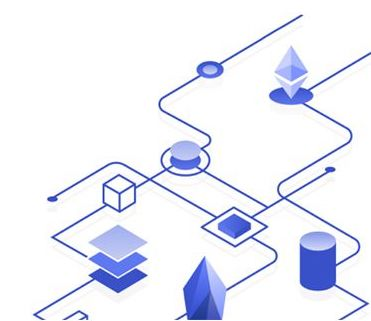
\includegraphics[width=150pt]{images/distributed_systems.jpg}\hspace*{\fill}
  \label{fig:polimi}
\end{figure} \\
}}
\date{Politecnico di Milano \\ Computer Science $\&$ Engineering | Fall 2019-2020}
\newcommand{\myparagraph}[1]{\paragraph{#1}\mbox{}\\[0.05in]}
\newcommand{\mydefinition}[1]{\textcolor{MidnightBlue}{\textit{"#1"}\\ \\}}
\begin{document}
\maketitle
\clearpage
\tableofcontents
\clearpage
\textcolor{Red}{! DISCLAIMER} \\
The only purpose of this document is to help students and the community to get prepared for exam. All the material included here has been taken from the slides used by the professor and then integrated with some additional notes taken personally by me, during classes. Thus, the books and various resources are the one specified in the Administration document published by the professor in his site:
\begin{itemize}
	\item A.S. Tanenbaum, M. van Steen. Distributed Systems: Principles \& Paradigms, 2nd ed. Prentice Hall, 2006 (disponibile anche in italiano)
	\item G. Coulouris, J. Dollimore, T. Kindberg. Distributed Systems: Concepts and Design (4th edition). Addison- Wesley, 2005
	\item M. Kleppmann. Designing Data-Intensive Applications: The Big Ideas Behind Reliable, Scalable, and Maintainable Systems. O’Really Media, 2017
	\item M.Hughes,M.Shoffner,D.Hammer.JavaNetworkProgramming,Manning,1999
	\item D. Lea. Concurrent Programming in Java: Design Principles and Patterns. Addison-Wesley (Java Series)
\end{itemize}
Special thanks to Luca Conterio who contributed with some exercises' solutions.
\clearpage
\section{ \LARGE Introduction}
Most applications we use today are "distributed". E-mail is probably the oldest and largest distributed application since it has billions of users and $\sim{2.5M}$ of emails per second. Another example is the Web, which counts $\sim{1B}$ registered web server names today. Google itself is a distributed system...
Why to distribute?
\begin{itemize}
  \item \textbf{Economics}: price/performance ratio in favor of distribution
  \item \textbf{Incremental} growth and load balancing: easier to evolve the system and use its resources uniformly
  \item \textbf{Inherent distribution}: banks, reservation services, distributed games, mobile apps
  \item \textbf{Reliability}: failure does not bring down the whole system
\end{itemize}
However, distributed systems are more complex than standard (centralized) ones. Building them is hard. Building them correctly is much harder. 
\textit{Perter Deutsch} listed the Eight Fallacies of Distributed Computing. Essentially it is a list of assumptions that usually occurs when everyone first build a distributed application. All prove to be false in the long run and all cause big trouble and painful learning experiences.
\begin{enumerate}
  \item The network is reliable
  \item Latency is zero
  \item Bandwidth is infinite
  \item The network is secure
  \item Topology doesn't change
  \item There is one administrator
  \item  Transport cost is zero
  \item The network is homogeneous
\end{enumerate}
\subsection{What is a distributed system?}
\textit{"A distributed system is a system in which hardware or software components located at networked computers communicate and coordinate their actions only by passing messages"} \\ (G. Coulouris, J. Dollimore, T.Kindberg) \\ \\
\textit{"A distributed system is a collection of independent computers that appears to its users as a single coherent system"} \\ (A.S. Tanenbaum, M. van Steen) \\
In a distributed system the various components communicates only with message passing, while a parallel system can also communicate through shared memory. In a DS there is no shared clock, neither shared memory but only message passign through a network. \pagebreak
 \begin{figure}[h!]
 \hfill 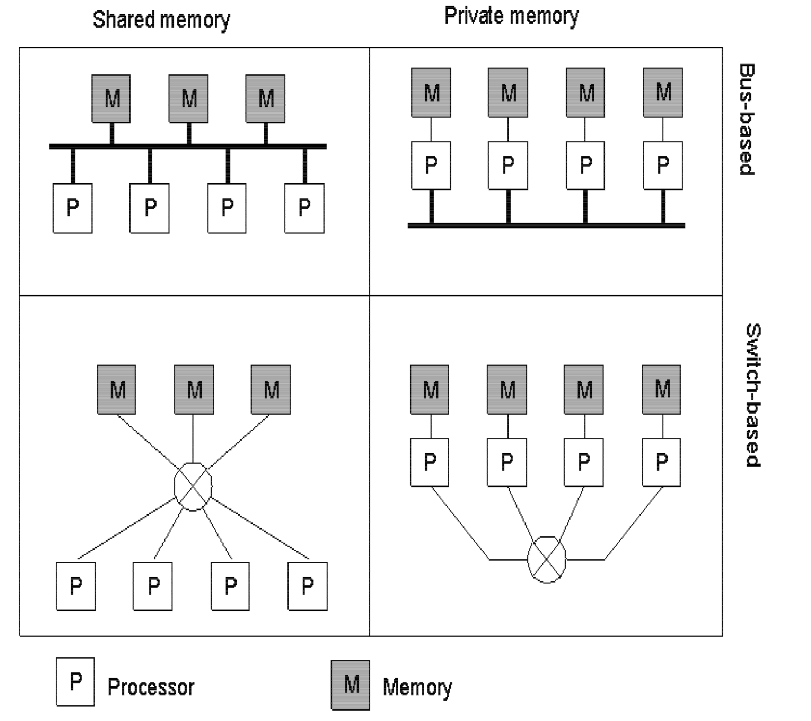
\includegraphics[width=150pt]{images/par_dis.png}\hspace*{\fill}
  \caption{Parallel computing (left column) vs. distributed computing (right column)}
  \label{fig:par_dis}
\end{figure} \\
There are two types of distributed systems:
\begin{itemize}
	\item \textbf{Network/OS} based distributed system: leverages the fact that systems implicitly offer some middleware technologies at low level such as TCP.
	\item \textbf{Middleware} based distributed system: middleware offers services that hide part of the distribution, letting the different machine appearing as a single one.
\end{itemize}
\begin{figure}[h!]
\centering
\begin{minipage}{.5\textwidth}
  \centering
  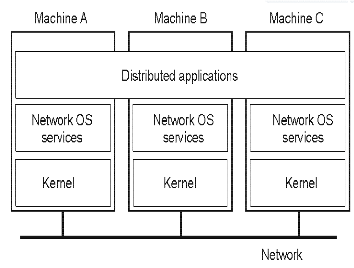
\includegraphics[width=.6\linewidth]{images/network.png}
  \captionof{figure}{Network/OS based}
  \label{fig:network}
\end{minipage}%
\begin{minipage}{.5\textwidth}
  \centering
  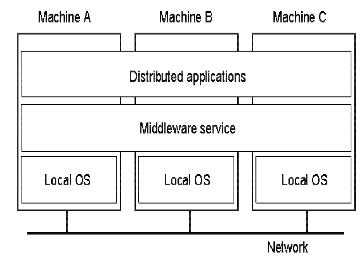
\includegraphics[width=.5\linewidth]{images/middleware.png}
  \captionof{figure}{Middleware based}
  \label{fig:middleware}
\end{minipage}
\end{figure} 
\subsection{Defining Features and Challenges}
\subsubsection{Features}
\begin{itemize}
	\item \textbf{Concurrency}: in centralized systems, concurrency is a design choice. In distributed systems, it is a fact of life to be dealt with: computer are always (co)-operating at the same time.
	\item \textbf{Absence of a global clock}: in centralized systems, the computer's physical clock can be used for the purpose of synchronization. In distributed systems, clocks are many and not necessarily synced.
	\item \textbf{Independent (and partial) failures}: centralized systems typically fail completely. Distributed systems fail only partially, and often due to communication. Each component can fail independently leaving the others still running. Hard/impossible to detect failures. Moreover, recovery is made more complicated by the fact that the application state is itself distributed.
\end{itemize}
\subsubsection{Challenges}
\begin{itemize}
	\item \textbf{Heterogeneity}: of hosts, platforms, networks, protocols, languages, ...
	\item \textbf{Openness}: a distributed system should foster interoperability through standard access rules. Protocols and interfaces play a key role.
	\item \textbf{Security}: the ease of attaching a node to the system can be exploited maliciously.
	\item \textbf{Scalability}: use decentralized algorithms to allow the system to grow with the lowest possible impact on performance. Performance should decrease linearly with growth.
	\item \textbf{Failure handling}: hosts can fail, links are unreliable, the two are usually indistinguishable, global state complicates matters. Detecting, masking, tolerating, recovery from failures.
	\item \textbf{Concurrency}: synchronization without a physical clock and without a shared memory.
	\item \textbf{Transparency}: hide the most to simplify the life of programmers/users.
\end{itemize}
\pagebreak
\section{\LARGE Modelling}
\subsection{The software architectures of a distributed system}
\begin{itemize}
	\item \textbf{Network OS based}:  build on basic facilities offered by OS (Socket, TCP, ...) without any additional library
	\begin{itemize}
		\item The network OS provides the communication services
		\item Different machines may have different networks OSes
		\item Masking platform differences is up to the programmer
	\end{itemize}
	\item \textbf{Middleware based}: a layer of software provides communication (RPC, RMI) coordination (synchronize operations) and administration (who may access some data) facilities
	\begin{itemize}
		\item The middleware provides advanced communication, coordination, and administration services
		\item It masks most of the platform differences
	\end{itemize}
\end{itemize}
Middleware provides "business-unaware" (i.e., general purpose) services through a standard API, which raises the level of the communication activities of applications. Usually it provides:
\begin{itemize}
	\item Communication and coordination services
	\begin{itemize}
		\item Synchronous (Java RMI) and asynchronous (message passing)
		\item Point-to-point or multicast
		\item Masking differences in the network OS
	\end{itemize}
	\item Special application services
	\begin{itemize}
		\item Distributed transaction management, groupware and work flow services, messaging services, notification services, ...
	\end{itemize}
	\item Management services
	\begin{itemize}
		\item Naming, security, failure handling, ...
	\end{itemize}
\end{itemize}
\subsection{The run-time architecture}
The run-time (system) architecture of a distributed system identifies the classes of components that build the system, the various types of connectors, and the data types exchanged at run-time. \\
Modern distributed systems often adopt one among a small set of well known \textbf{architectural styles}:
\begin{itemize}
	\item Client-server
	\item Service Oriented
	\item REST
	\item Peer-to-peer
	\item Object-oriented
	\item Data-centered
	\item Event-based
	\item Mobile code
	\item CREST
\end{itemize}
\subsubsection{Client-server}
The most common architectural style today. \\ Here communication is \textbf{message based} (or RPC) and  components have different roles:
\begin{itemize}
	\item \textbf{Servers} provide a set of services through a well defined API and they are passive (just wait for client invocations)
	\item Users access those services through \textbf{clients}
\end{itemize}
There may happen that the server is composed by \textbf{several layers} (at least two) such that the client requests to the first-tier (layer) and the first-ltier itself invoke a second-tier. The response will follow the reverse path. 
\begin{figure}[h!]
\centering
\begin{minipage}{.5\textwidth}
  \centering
  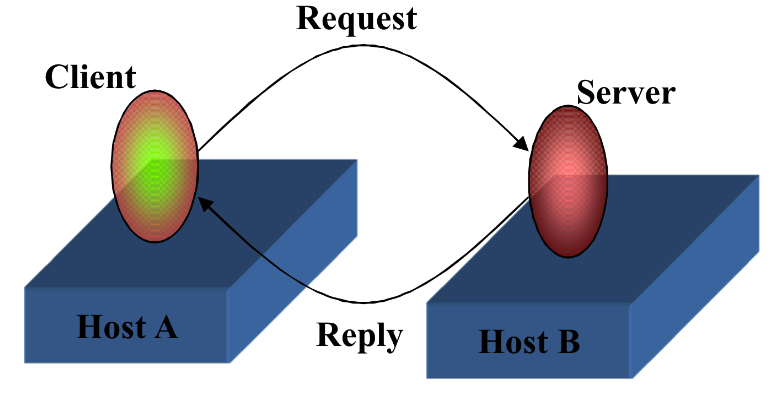
\includegraphics[width=.6\linewidth]{images/single-tier.png}
  \captionof{figure}{Single-tier application}
  \label{fig:single-tier}
\end{minipage}%
\begin{minipage}{.5\textwidth}
  \centering
  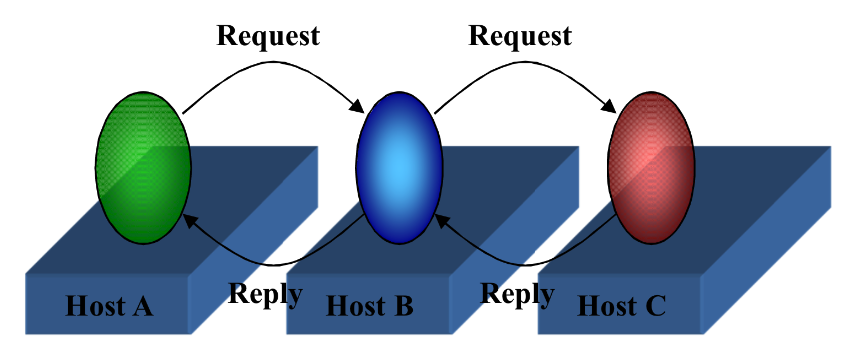
\includegraphics[width=.5\linewidth]{images/multi-tier.png}
  \captionof{figure}{Three-tiers application}
  \label{fig:multi-tier}
\end{minipage}
\end{figure} 
\\ In general, the services offered by a distributed application can be partitioned in three classes: user interface, application services, storage services. \textbf{Multi-tiered} client-server applications can be classified looking at the way such services are assigned to the different tiers.
\begin{figure}[h!]
\centering
\begin{minipage}{.5\textwidth}
  \centering
  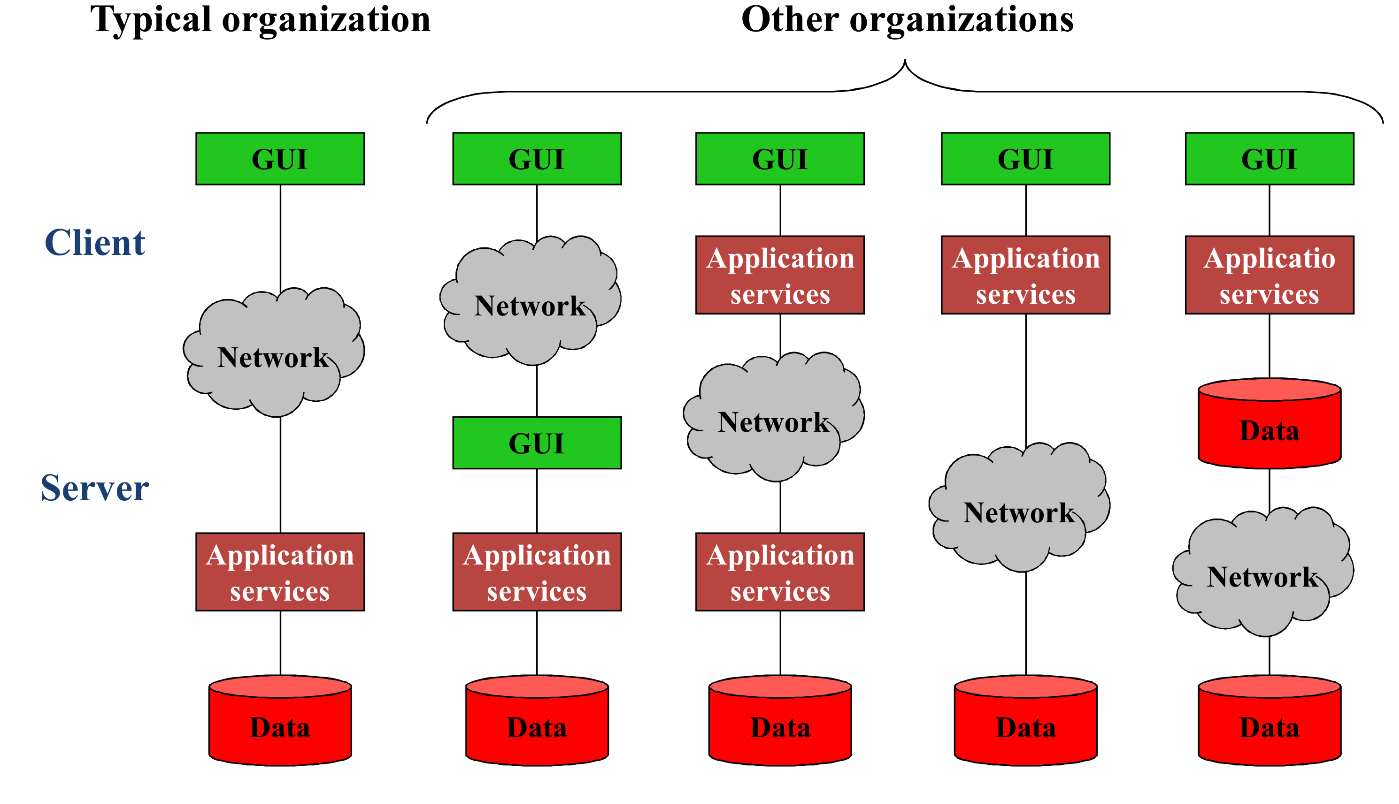
\includegraphics[width=.8\linewidth]{images/two-tiered.png}
  \captionof{figure}{Two-tiered architectures}
  \label{fig:two-tiered}
\end{minipage}%
\begin{minipage}{.5\textwidth}
  \centering
  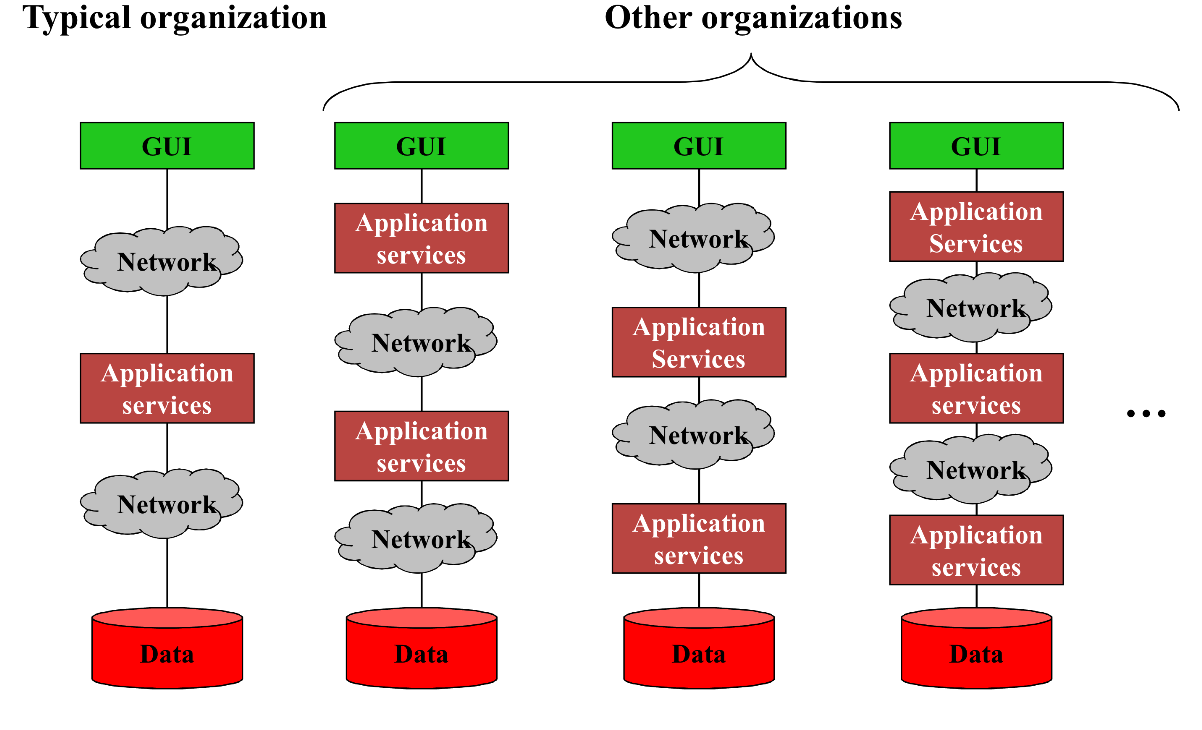
\includegraphics[width=.8\linewidth]{images/three-tiered.png}
  \captionof{figure}{Three-tiered architectures}
  \label{fig:three-tier}
\end{minipage}
\end{figure} 
\pagebreak
\subsubsection{Service Oriented}
 \begin{figure}[h!]
 \hfill 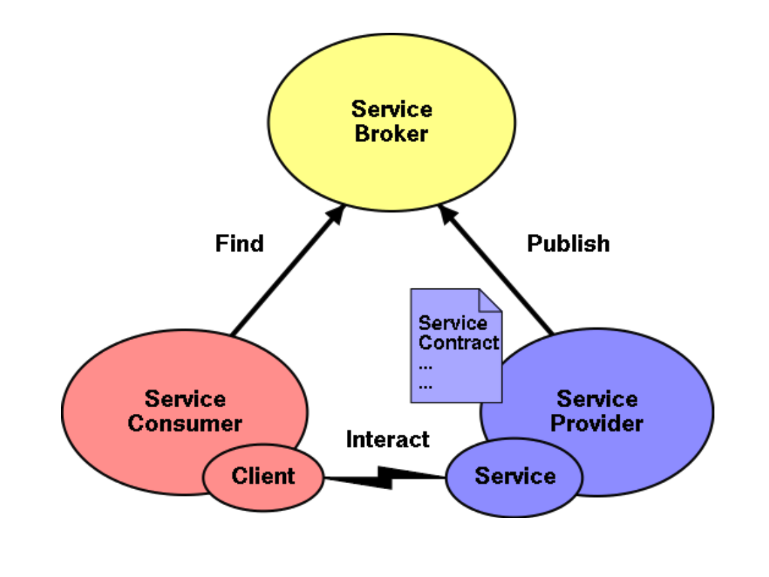
\includegraphics[width=150pt]{images/service-oriented.png}\hspace*{\fill}
  \caption{Service-oriented architecture}
  \label{fig:fsa1}
\end{figure}
The \textbf{Service Oriented} architecture is a specific case of client-server and it is built around the concepts of \textit{services, service providers, service consumers, service brokers}. \\ \textbf{Services} represent loosely coupled units of functionality exported by service providers. \textbf{Brokers} holder the descriptions of available services to be searched by interested \textbf{consumers} which bind and invoke the services they need. \textit{Orchestration} is the process of invoking a set of services in an ad-hoc workflow to satisfy a given goal.
\begin{itemize}
	\item \textbf{Service provider} is the server that provides the service. The same service can be provided by different servers.
	\item \textbf{Service consumer} is the client. A service consumer may be also a service provider.
	\item \textbf{Service broker} provides business-unaware services, typically the list of available services. The broker reduces the dependency that exists in client-server system because the client needs to know only the address of the broker and no more the address of the server.
\end{itemize}
\textit{Web services} are a possible incarnation of service oriented architecture. A web service is a software system designed to support interoperable machine-to-machine interaction over a network. Web service operations are invoked through \textit{SOAP}, a protocol based on XML, which defines the way messages (operation calls) are actually exchanged between providers and consumers. Usually HTTP is used.
\subsubsection{REST}
\textbf{REpresentational State Transfer (REST)} is a set of principles that define how Web standards are supposed to be used, which often differs quite a bit from what many people actually do. \\
The \textbf{key goals} of REST include:
\begin{itemize}
	\item Scalability of component interactions
	\item Generality of interfaces
	\item Independent deployment of components
	\item Intermediary components to reduce latency, enforce security and encapsulate legacy systems.
\end{itemize}
The main \textbf{constraints} of REST are:
\begin{itemize}
	\item Interactions are client-server and \textit{stateless}. This means that the history is not accumulated with time, giving an advantage in term of scalability. Eventually a caching service to reduce latency in case the clients sends multiple time the same request, avoiding the server to execute multiple time the same functions.
	\item The data within a response to a request must be implicitly or explicitly labeled as cacheable or non-cacheable. The ability of caching data is key to provide scalability.
	\item Each component cannot "see" beyond the immediate layer with which they are interacting (REST is layered).
	\item Clients must support code-on-demand (basically JavaScript on the Web)
	\item Components expose a \textit{uniform interface}: GET, POST, PUT, DELETE.
\end{itemize}
The uniform interface exposed by components must satisfy four constraints:
\begin{itemize}
	\item Identification of resources: each resource must have an id (usually an URI) and everything that have an id is a valid resource
	\item Manipulation of resources through representations: REST components communicate by transferring a representation of a resource in a format matching one of an evolving set of standard data types (e.g., XML), selected dynamically based on the capabilities or desires of the recipient and the nature of the resource. A representation consists of data and metadata describing the data.
	\item Self-descriptive messages: control data defines the purpose of a message between components, such as the action being requested or the meaning of the response. 
	\item Hypermedia as the engine of application state: clients move from a state to another each time process a new representation, usually linked to other representation through hypermedia links.
\end{itemize}
\subsubsection{Peer-to-peer}
In \textbf{peer-to-peer} applications all components play the same role, thus there is no distinction between clients and servers. \\  The main reason behind P2P is that client-server does not scale well due to the centralization of service provision and management. Furthermore, the server is also a single point of failure. P2P leverages off the increased availability of broadband connectivity and processing power at the end-host to overcome such limitations. \\
P2P promotes the sharing of resources and services through direct exchange between peers. Resources can be:
\begin{itemize}
	\item Processing cycles (SETI@home)
	\item Collaborative work (Skype)
	\item Storage space (Freenet)
	\item Network bandwidth (ad hoc networking, internet)
	\item Data (most of the rest)
\end{itemize}
In the end, as Clay Shirky and O'Reilly said, P2P fundamental difference is that it \textit{"takes advantage of resources at the edges of the network"}.
\subsubsection{Object-Oriented}
In \textbf{Object-Oriented} architecture, the distributed components encapsulate a data structure providing an API to access and modify it. Each component is responsible for ensuring the integrity of the data structure it encapsulates and the internal organization of such data structure is hidden to the other components. The components interact through RPC (remote procedure call). \\
Object-Oriented architecture can be seen as a special case of P2P system because each component is a peer in the sense that both provide and use services. Furthermore, OO is the opposite of REST because it is \textit{stateful}. \\
The main advantages of OO are:
\begin{itemize}
	\item Information hiding hides complexity in accessing/managing the shared data
	\item Encapsulation plus information hiding reduce the management complexity
	\item Objects are easy to reuse among different applications
	\item Legacy components can be wrapped within objects and easily integrated in new applications
\end{itemize}
\subsubsection{Data-centered}
\begin{figure}[h!]
 \hfill 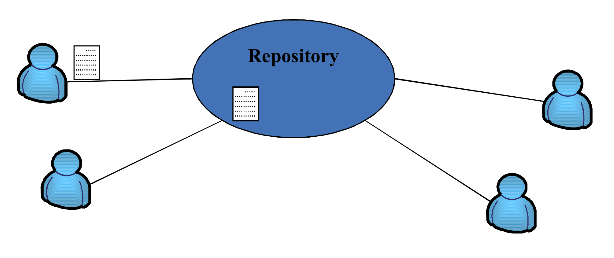
\includegraphics[width=150pt]{images/data-centered.png}\hspace*{\fill}
  \caption{Data-centered architecture}
  \label{fig:data-centered}
\end{figure}
In \textbf{Data-centered} applications components communicate through a common (usually passive) repository. Data can be added to the repository or taken (moved or copied) from it. The communication with the repository is (usually) through RPC. \\
Communication properties:
\begin{itemize}
	\item \textbf{Anonymous}: when clients send a message, they don't know who will receive that. There is no coupling between sender and receiver.
	\item \textbf{Persisent}: when data is sent, it remains in the shared space until someone gets it.
\end{itemize}
\textit{Example: Linda and tuple spaces}
\begin{figure}[h!]
 \hfill 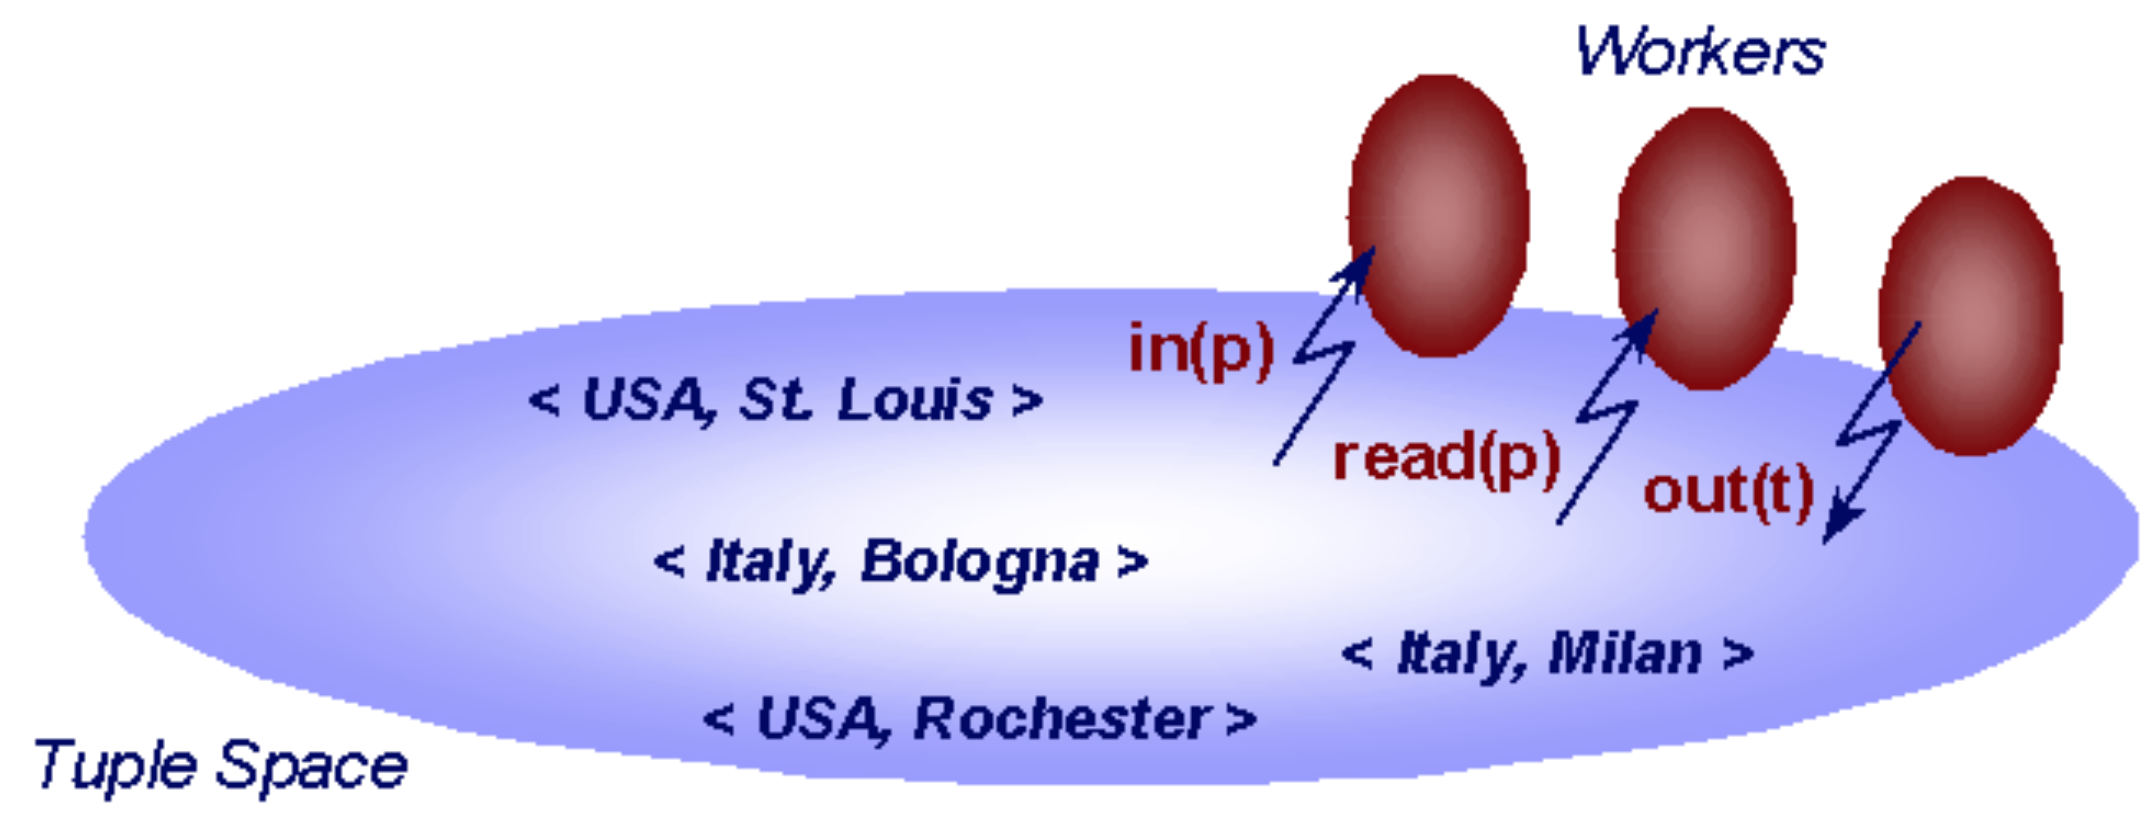
\includegraphics[width=170pt]{images/linda.png}\hspace*{\fill}
  \caption{Three Linda processes interacting with a single tuple space with the standard Linda operations.}
  \label{fig:linda}
\end{figure} \\
Linda is a data sharing model proposed in the 80s by Carriero and Gelernter, mostly used for parallel computation.
\pagebreak
\\ Linda in a nutshell:
\begin{itemize}
	\item The communications is persistent, implicit, content-based, generative.
	\item Data is contained in ordered sequences of typed fields (\textit{tuples})
	\item Tuples are stores in a persistent, global shared space (\textit{tuple space})
	\item Standard operations:
	\begin{itemize}
		\item \textbf{out(t)}: writes tuple $t$ in tuple space
		\item \textbf{rd(p)}: returns a copy of a tuple matching the \textit{pattern p}, if it exists; blocks waiting for a matching tuple otherwise.
		\item \textbf{in(p)}: like $rd(p)$, but withdraws the matching tuple from the tuple space
		\item \textbf{eval(a)}: some implementations provide this operation which inserts the tuple generated by the execution of process $a$
	\end{itemize}
\end{itemize}
There are some architectural issues with Linda:
\begin{itemize}
	\item The tuple space model is not easily scaled on a wide-area network because is not easy to store/replicate tuples and route queries efficiently.
	\item The model is proactive, this means that it can only ask for data, there is no notification when new data is produced.
\end{itemize}
\subsubsection{Event-based}
In \textbf{Event-based} architecture components collaborate by exchanging information about occurrent \textit{events}. In particular components:
\begin{itemize}
	\item \textbf{publish} notifications about the events they observe, or
	\item \textbf{subscribe} to the events they are interested to be notified about
\end{itemize}
Communications is: 
\begin{itemize}
	\item Purely message based
	\item Asynchronous
	\item Multicast
	\item Implicit
	\item Anonymous
\end{itemize}
While in Data-center the communication is persistent, in Event-based architecture the communication is transient. Furthermore, the model is \textbf{reactive}, this means that whenever a new data is produced, all the clients interested will get it.
\pagebreak
\subsubsection{Mobile code}
\textbf{Mobile code} architecture is based on the ability of relocating the components of a distributed application at run-time. There are different models depending on the original and final location of resources, know-how (the code) and computational components (including the state of execution).
\begin{figure}[h!]
 \hfill 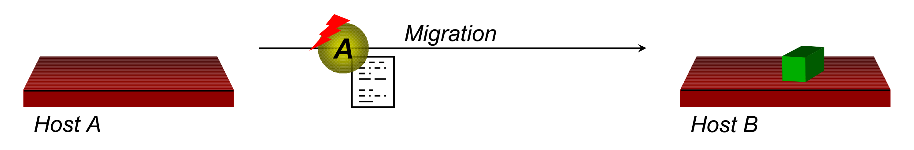
\includegraphics[width=170pt]{images/mobile-code.png}\hspace*{\fill}
  \caption{Code migration from host A to host B}
  \label{fig:mobilecode}
\end{figure} \\
There are four different mobile code \textbf{paradigms}:
\begin{itemize}
	\item \textbf{Client-Server}: both code and execution capabilities are server side.
	\item \textbf{Remote evaluation}: who request the service has the code, the other side executes it and sends back the evaluation. There may be a problem of security because server is made execute external code. An example is the Postcript printing.
	\item \textbf{Code on demand}: who request the service has everything except for the code, so the code is asked and then executed locally. Clients should be able to execute code locally (JavaScript).
	\item \textbf{Mobile agent}: Someone has both code and data, but does not have the ability of processing. The partially evaluated code/data is sent to the other side to complete the execution (no practical examples).
\end{itemize}
\begin{figure}[h!]
\centering
\begin{minipage}{.5\textwidth}
  \centering
  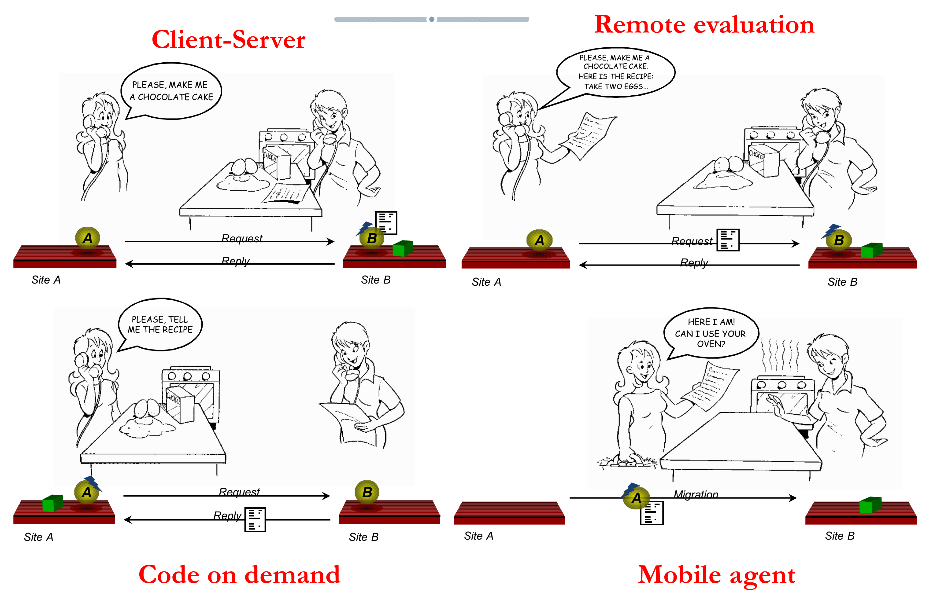
\includegraphics[width=.9\linewidth]{images/mobile-paradigms2.png}
  \captionof{figure}{Mobile code paradigms in sketch}
  \label{fig:mobilepvisual}
\end{minipage}%
\begin{minipage}{.5\textwidth}
  \centering
  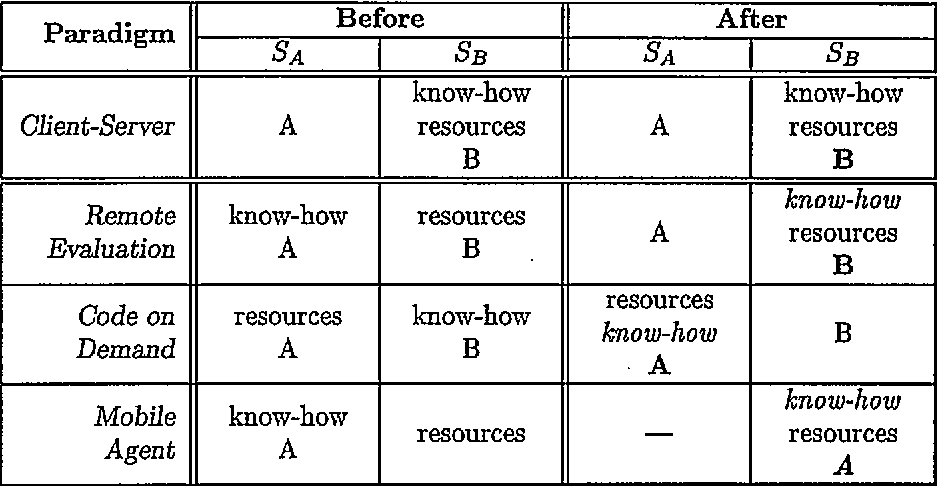
\includegraphics[width=.9\linewidth]{images/mobile-paradigms.png}
  \captionof{figure}{Mobile code paradigms table}
  \label{fig:mobileptable}
\end{minipage}
\end{figure} 
To mention \textbf{function languages (lambda functions)} that are in the middle between Remote evaluation and Mobile agent. \\
Mobile code technologies are of two kinds:
\begin{itemize}
	\item \textit{Strong mobility}: the ability of a system to allow migration of both the code and the execution state of an executing unit to a different computational environment. Very few systems provide it (mobile agent).
	\item \textit{Weak mobility}: the ability of a system to allow code movement across different computational environments. This one is provided by several mainstream systems including Java, .Net, the Web (remote evaluation and code on demand). 
\end{itemize}
The main advantage of mobile code is that the ability to move pieces of code (or entire components) at run-time provides a great flexibility to programmers:
\begin{itemize}
	\item New versions of a component can be uploaded at run-time without stopping the application
	\item Existing components can be enriched with new functionalities
	\item New services can be easily added
	\item Existing services can be adapted to the client need
\end{itemize}
In cons, securing mobile code application is a mess.
\subsubsection{CREST}
\textbf{CREST (Computational REST)} joins together the concepts of REST with mobile code. This because REST is not sufficient to describle complex web 2.0 applications (e.g., those enabled by AJAX). \\
In CREST, instead of "representations", interacting parties exchange "computations", adding flexibility but also complexity.\\ \\
CREST axioms:
\begin{itemize}
	\item A resource is a locus of computations named by an URI
	\item The representation of a computation is an "expression" plus metadata to describe it
	\item All computations are context-free
	\item Only a few primitive operations are always available, but additional per-resource and per-computation operations are also encouraged.
	\item The presence of intermediaries is promoted
\end{itemize}
\subsection{The interaction model}
\subsubsection{Distributed algorithms}
Traditional programs can be describe in terms of the algorithm they implement, where steps are strictly sequential and (usually) process execution speed influence performance, only. \\
Distributed systems are composed of many processes, which interact in complex way, and their behavior can be described by a \textit{distributed algorithms}. Since \textbf{there is not a global-clock}, it is not guaranteed the sequential execution of a distributed algorithm. Thus, the same set of algorithm executed by the same set of components with the same set of processes with different clocks may result in different behaviors.
The behavior of a distributed system is influenced by several factors:
\begin{itemize}
	\item The rate at which each process proceeds
	\item The performance of the communication channels
	\item The different clock drift rates
\end{itemize}
Our goal is to write an algorithm for each single process such that the systems remains correct independently on the speed of the network, the speed of the clock and the errors. \\
\subsubsection{Interaction model}
To formally analyze the behavior of a distributed system we must distinguish between:
\begin{itemize}
	\item \textbf{Synchronous distributed systems}: 
	\begin{itemize}
	\item Each step of a process we know the minimum and maximum time it may take to complete (lower and upper bounds)
	\item Each message is received within a maximum time
	\item Each process has a maximum clock that may reach
\end{itemize}
	\item \textbf{Asynchronous distributed systems}: there are no bounds for process executions speeds, message transmission delays and clock drift rates
\end{itemize}
Any solution that is valid for an asynchronous distributed system is also valid for a synchronous one (but the vice versa is clearly false). In general we assume that our system is synchronous using large bounds so that the crash/error rate is limited.
\subsubsection{The pepperland example}
\begin{figure}[h!]
 \hfill 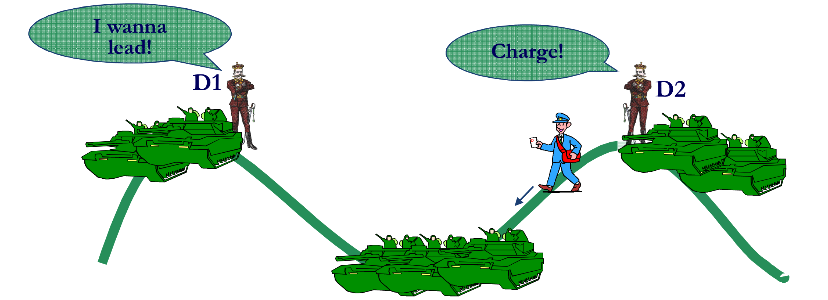
\includegraphics[width=170pt]{images/pepperland.png}\hspace*{\fill}
 
  \label{fig:pepperland}
\end{figure}
The pepperland example is used to describe the \textbf{agreement problem} that is common in distributed applications. \\ The pepperland divisions are safe as long as they remain in their encampments. If both charge at the same time they win, otherwise they loose. Generals need to agree on:
\begin{itemize}
	\item Who will lead the charge
	\item When the charge will take place
\end{itemize}
We consider the case when messengers are able to walk from an hill to another without being captured by the enemies (messages cannot be lost). \\
A possible algorithm may consists in both divisions sending random number. Once received, the one who sent the higher number will lead the charge. In case of equal numbers, repeat. Eventuall somebody will charge. \\
It is possible to agree on who will lead the charge in both asynchronous and synchronous pepperland. \\
It is not possible to agree on charge in asynchronous pepperland because there aren't any bound on the time that is required by the messenger to arrive. This means that we cannot know if the message has been lost or it is still arriving. \pagebreak \\
In synchronous pepperland it is possible to determine the maximum difference between charge times.
\begin{enumerate}
	\item Let $min$ and $max$ be the range of message transmission times
	\item The leader sends a message "charge", wait $min$ minutes then charge
	\item On receiving the "charge" message the other general immediately charge
	\item The second division may charge later the the first one but no more than $(max-min)$ minutes
	\item If we know that the charge will last longer then the victory is guaranteed
\end{enumerate}
\subsection{The failure model}
\subsubsection{Failure model}
Both processes and communication channels may fail. The \textbf{failure model} defines the ways in which failure may occur to provide a better understanding of the effects of failures. We distinguish between:
\begin{itemize}
	\item \textbf{Omission failure}: 
	\begin{itemize}
		\item Processes: fail or crash
		\item Channels: may encounter \textit{send omission} (losing packet while traversing the OS and network), \textit{channel omission} (losing packet while traversing the physical network) and \textit{receiving omission} (losing packet while traversing network and OS on the other side)
	\end{itemize}
	\item \textbf{Byzantine (or arbitrary) failures}:
	\begin{itemize}
		\item Processes: may omit intended processing steps or add more
		\item Channels: message content may be corrupted, non-existent messages may be delivered, or real messages may be delivered more than once
	\end{itemize}
	\item \textbf{Timing failures}:
	\begin{itemize}
		\item Occur when one of the time limits defined for the system is violated (apply to synchronous systems only)
		\end{itemize}
\end{itemize}
Omission failures are more common for processes, while Byzantine failures are more common for channels.
\subsubsection{Failure detection in pepperland}
In synchronous pepperland is easy to detect if one of the two divisions has been attacked and defeated by enemies:
each division periodically send a messenger to the other saying "I am still here"; when no messengers arrive for longer than $max$ minutes we can conclude that the other division has been defeated. \\
In asynchronous pepperland we cannot distinguish whether the other division has been defeated or the time for the messenger to cross the valley is just very long.
\subsubsection{Agreement in "failing pepperland"}
Suppose the messengers can be captured by enemies. Can the two generals send messengers so that they both consistently decide to charge or surrender? \\
Reaching an agreement on one of the two possible decisions requires the successful arrival of at least one message. \\ \\ Consider scenario A in which the fewest delivered messages that will result in agreement to attack are delivered. Let scenario B be the same as A except that the last message delivered in A is lost in B, and any other messages that might be sent later are also lost. Suppose that this last message is from General 1 to General 2. \\ General 1 sees the same messages in both scenarios, so he definitely attacks. However, the minimality assumption of A implies that General 2 cannot also decide to attack in scenario B, so he must make a different decision. Hence General 1, not being sure its last message arrived, has wrongly decided to attack (both in scenarios A and B). \textbf{The problem is unsolvable}.
\pagebreak
\section{\LARGE Communication}
\subsection{Fundamentals}
\subsubsection{Protocols and protocol stacks}
The \textbf{Open Systems Interconnection model (OSI model)} is a conceptual model that characterizes and standardizes the communication functions of a telecommunication or computing system without regard to its underlying internal structure and technology. Its goal is the interoperability of diverse communication systems with standard communication protocols. The model partitions a communication system into abstraction layers. The original version of the model had seven layers.
\begin{figure}[h!]
 \hfill 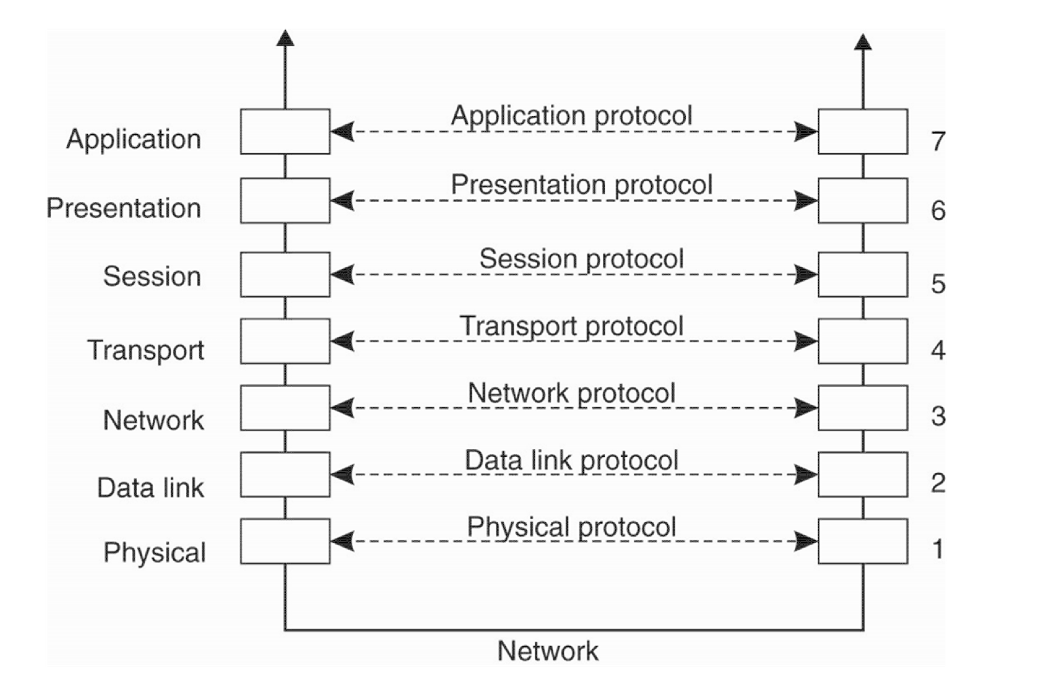
\includegraphics[width=160pt]{images/osi.png}\hspace*{\fill}
 \caption{Communication in the OSI Model}
  \label{fig:osi}
\end{figure}
\begin{itemize}
	\item Low level layers:
		\begin{itemize}
			\item Physical layer: describes how bits are transmitted between two directly connected nodes
			\item Data link layer: describes how a series of bits is packed into a frame to allow for error and flow control
			\item Network layer: describes how packets in a network of computers are to be routed
		\end{itemize}
	\item Transport layer: describes how data is transmitted among two nodes, offering a service independent at lower layers; it provides the actual communication facilities for most distributed systems (TCP and UDP)
	\item High level layers: merged together in the current, Internet practice
\end{itemize}
\begin{figure}[h!]
 \hfill 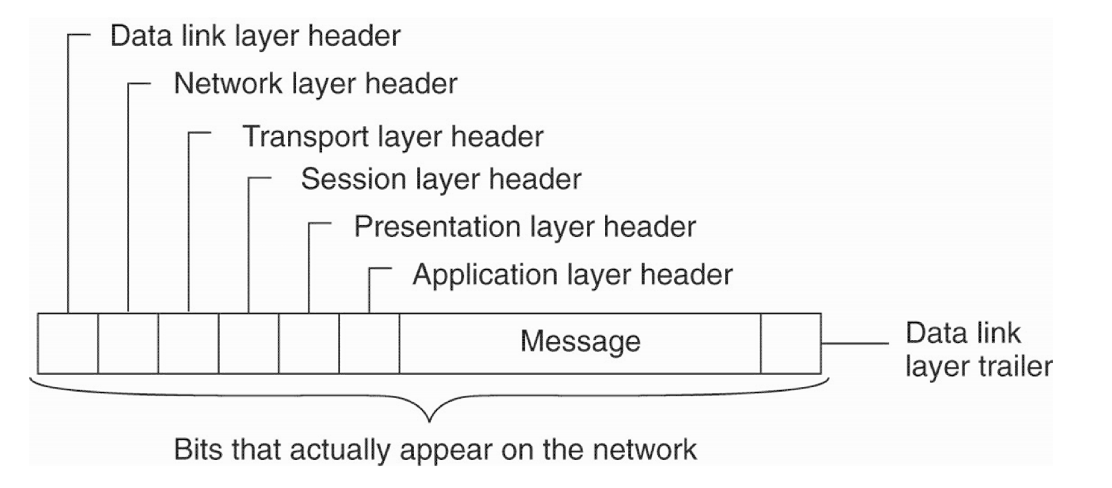
\includegraphics[width=160pt]{images/encapsulation.png}\hspace*{\fill}
 \caption{Layered protocols encapsulation}
  \label{fig:encapsulation}
\end{figure}
The packet is the basic unit of information transferred across a network, consisting, at a minimum, of a header with the sending and receiving hosts' addresses, and a body with the data to be transferred. As the packet travels through the TCP/IP protocol stack, the protocols at each layer either add or remove fields from the basic header. When a protocol on the sending host adds data to the packet header, the process is called data \textbf{encapsulation}.
\subsubsection{Middleware}
\textbf{Middleware} can be considered as an additional layer. It includes common services and protocols that can be used by many different applications:
\begin{itemize}
	\item (Un)marshaling of data, necessary for integrated systems
	\item Naming protocols, to allow easy sharing of resources
	\item Security protocols for secure communication
	\item Scaling mechanisms, such as for replication and caching
\end{itemize}
Middleware may offer different form of communication:
\begin{itemize}
	\item \textit{Transient vs. Persistent}:
	\begin{itemize}
		\item Transient: the communication only happens if the two parties are available and active at the same time (UDP)
		\item Persistent: the communication happens also if one of the two parties is not active, and eventually there is a database in the middle that stores data (TCP, e.g., Whatsapp)
	\end{itemize}
	\item \textit{Synchronous vs. Asynchronous}:
	\begin{itemize}
		\item Synchronous: synchronization witht the middleware. A phone call is synchronous because if A is calling B, the communication happens only if B answers and "synchronize"
		\item Asynchronous: no need of synchronization between clients
	\end{itemize}
\end{itemize}
\begin{figure}[h!]
 \hfill 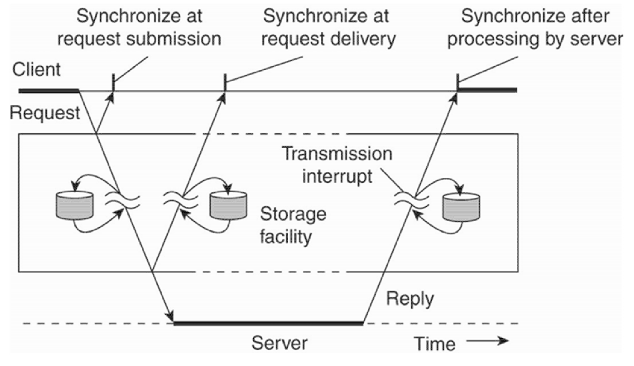
\includegraphics[width=160pt]{images/middleware-sync.png}\hspace*{\fill}
 \caption{Different types of synchronization}
  \label{fig:middleware-sync}
\end{figure}
\pagebreak
\subsection{Remote procedure call}
\subsubsection{Fundamentals}
\textbf{Remote Procedure Call (RPC)} is a protocol that one program can use to request a service (function) from a program located in another computer on a network without having to understand the network's details. The function parameters to be used are embedded in the request. \\
RPC uses different mechanisms to pass parameters:
\begin{itemize}
	\item By \textit{value}: like in C when passing basic data types
	\item By \textit{reference}: like in  C when passing pointers (array) or in Java when passing objects
	\item By \textit{copy/restore}: similar but slightly different than previous one
\end{itemize}
\begin{figure}[h!]
\centering
\begin{minipage}{.5\textwidth}
  \centering
  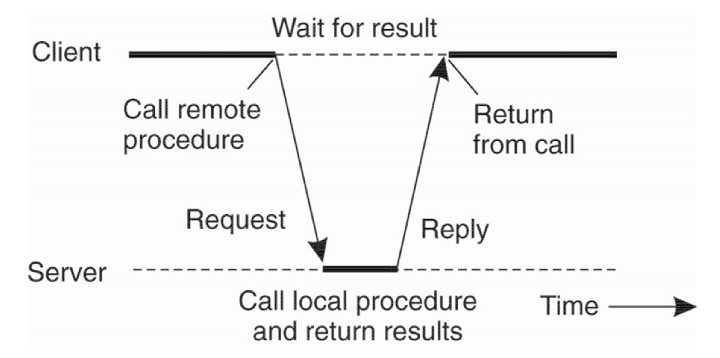
\includegraphics[width=.9\linewidth]{images/rpc.png}
  \captionof{figure}{RPC communication}
  \label{fig:rpc}
\end{minipage}%
\begin{minipage}{.5\textwidth}
  \centering
  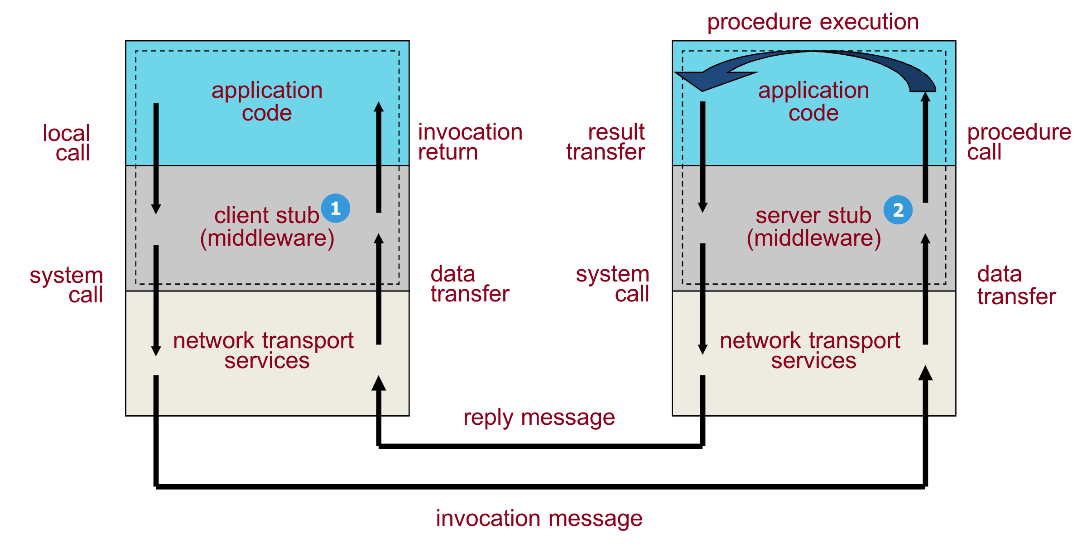
\includegraphics[width=.9\linewidth]{images/rpc2.png}
  \captionof{figure}{RPC: how it works}
  \label{fig:rpc2}
\end{minipage}
\end{figure} 
In Figure.18 the middleware "encodes" the parameters in a standardized packet called \textit{stub} and then sends it in the network. Once received, the packet is extracted from the stub and it is passed to the application that processes the execution. Finally, a response is sent back. \\
\begin{figure}[h!]
 \hfill 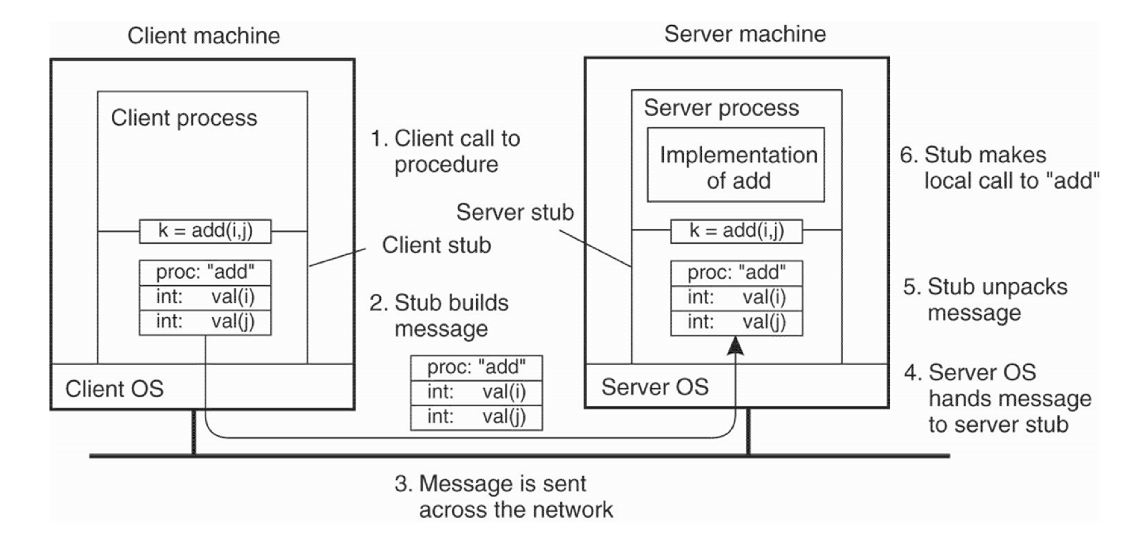
\includegraphics[width=250pt]{images/rpc3.png}\hspace*{\fill}
 \caption{RPC in details}
  \label{fig:rpc3}
\end{figure} \\
Passing a parameter poses two problems:
\begin{itemize}
	\item \textbf{Serialization}: structured data (e.g., structs, objects) must be ultimately flattened in a byte stream
	\item \textbf{Marshalling}: hosts may use different data representations (e.g., little endians vs. big endians) and proper conversions are needed
\end{itemize}
Thanks to middleware, the marshalling and serialization code is automatically generated and becomes part of the stub. This is enabled by a language/platform independent representation of procedure's signature, written using an \textbf{Interface Definition Language (IDL)}, and also a data representation format to be used during communication. \\
The IDL raises the level of abstraction of the service definition: 
\begin{itemize}
	\item It separates the service interface from its implementation
	\item The language comes with "mappings" onto target languages (e.g., C, Pascal, Python)
\end{itemize}
Advantages:
\begin{itemize}
	\item Enables the definition of services in a language-independent fashion
	\item Being defined formally, an IDL description can be used to automatically generate the service interface code in the target language
\end{itemize}
Passing parameter \textbf{by reference} often is not supported because many languages do not provide the notion of reference, but only of pointer. A pointer is meaningful only within the address space of a process... A possibility is to use call by value/result instead of reference. 
\subsubsection{Sun and DCE implementations}
\textbf{Sun Microsystems' RPC} is the \textit{de facto} standard over the internet. It is at the core of NFS, and many other (Unix) services and it uses either TCP or UDP to transport data in a format specified by XDR (eXternal Data Representation). Parameters are passed only by copy (no pointers). \\
The \textbf{Distributed Computing Environment (DCE)} is a set of specifications and a reference implementation. It provides several service on top of RPC: 
\begin{itemize}
	\item Directory service
	\item Distributed time service
	\item Distributed file service
\end{itemize}
Security is provided through Kerberos. \\
Microsoft's DCOM and .Net are based on DCE. \\ \\
The main problem of RPC is \textbf{binding client to server}, finding out which server (process) provides a given service. Hard-wiring this information in the client code is highly undesirable. Actually, there are two distinct problems:
\begin{itemize}
	\item Find out where the server process is.
	\item Find out how to establish communication with it.
\end{itemize} 
\paragraph{Sun's solution}
Introduce a daemon process ($portmap$) that bind calls and server/ports. The server picks an available port and tells it to $portmap$, along with the service identifier. Clients contact a given $portmap$ and request the port necessary to establish communication. 
$portmap$ provides its services only to local clients, i.e. it solves only the second problem. The clients must know in advance where the service resides. However, a client can multicast a query to multiple or, even more sophisticated, a directory service can be integrated.
\paragraph{DCE's solution} 
The DCE daemon works like $portmap$. The directory server (aka binder daemon) enables location transparency: client need not to know in advance where the service is, they only need where the directory service is. In DCE, the directory service can be actually distributed to improve scalability over many servers.
\begin{figure}[h!]
 \hfill 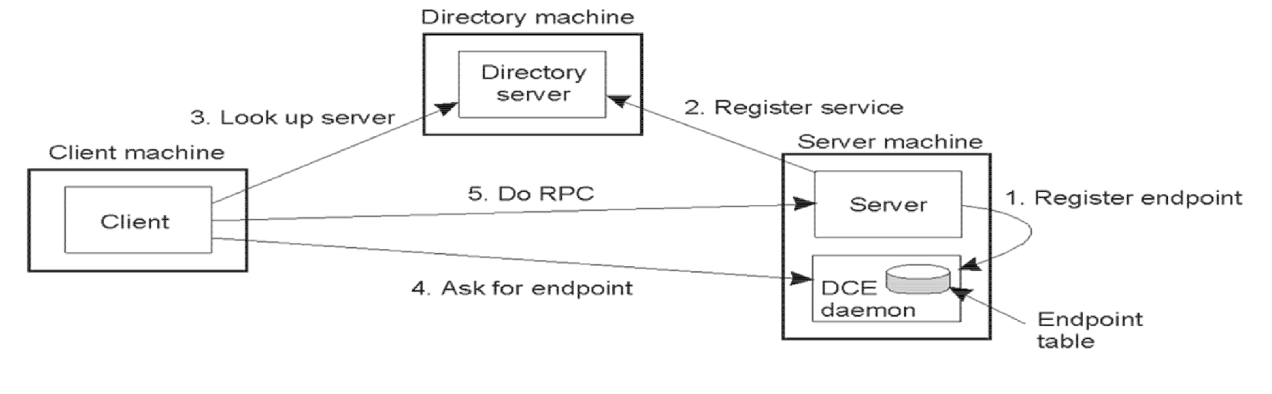
\includegraphics[width=200pt]{images/dce.png}\hspace*{\fill}
 \caption{DCE's architecture}
  \label{fig:dce}
\end{figure} \\
Another problem is that server processes may remain active even in absence of requests, wasting resources. This can be solved by introducing another (local) server daemon responsibile for a \textbf{dynamic activation} that:
\begin{itemize}
	\item Forks the process to serve the request
	\item Redirects the request if the process is already active
\end{itemize}
Clearly, the first request is served less efficiently because the startup may add an overhead but then the other requests will be served quickly. \\
In Sun RPC:
\begin{itemize}
	\item \textit{inetd daemon}, responsible for the server activation
	\item The mapping between requested service and server process is stored in a configuration file (\textit{/etc/services)}
\end{itemize}
It is natural to use the same primitives for inter-process communication, regardless of distribution. But using conventional RPC would lead to wasted resources because we don't need TCP/UDP on a single machine. \\
\textbf{Lightweight RPC} consists in message passing using local facilities, so instead of going through the network, they use the kernel. Thus, communication exploits a private shared memory region. For instance, copy/paste is implemented through RPC because we need to pass a complex data structure from one process to another. \\
Lightweight RPC invocation:
\begin{enumerate}
	\item Client stub copies the parameters on the shared stack and then performs
	\item Kernel does a context switch, to execute the procedure in the server
	\item Results are copied on the stack and another system call + context switch brings execution back to the client
\end{enumerate}
Advantages:
\begin{itemize}
	\item Use less threads/processes (no need to listen on a channel)
	\item 1 parameter copy instead of 4 (2 x ($stub \rightarrow kernel + kernel \rightarrow stub$))
\end{itemize}
Similar concepts used in practice in DCOM and .Net. \pagebreak \\
RPC preserves the usual call behavior: the caller is suspended until the callee is done (synchronous). Potentially wastes client resources:
\begin{itemize}
	\item Evident if no return value expected
	\item In general, concurrency could be increased
\end{itemize}
There are many variants of \textbf{asynchronous RPC} (with different semantics):
\begin{itemize}
	\item If no result is needed execution can resume after an acknowledgement is received from the server. One-way RPC returns immediately.
	\item To deal with results, the callee may (asynchronously) invoke the caller back, or invocation may return immediately a \textit{promise} (or \textit{future}), later polled by the client to obtain the result. 
\end{itemize}
\begin{figure}[h!]
\centering
\begin{minipage}{.3\textwidth}
  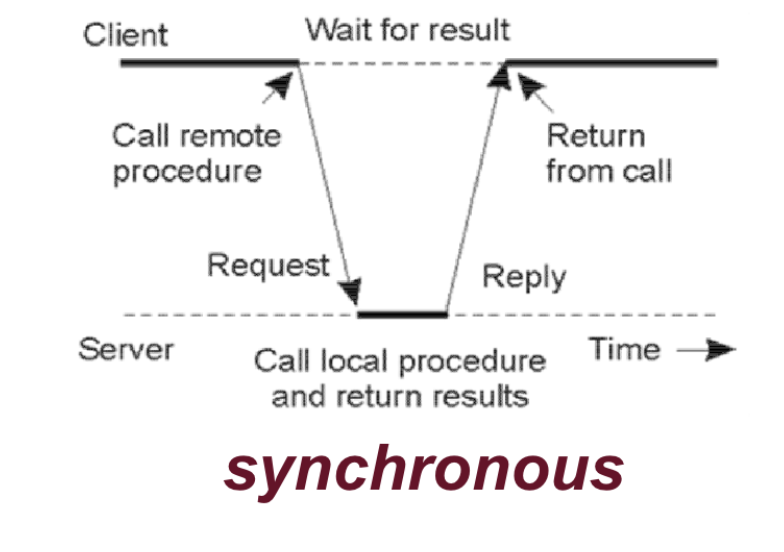
\includegraphics[width=.9\linewidth]{images/sync.png}
  \label{fig:sync}
\end{minipage}%
\begin{minipage}{.3\textwidth}
  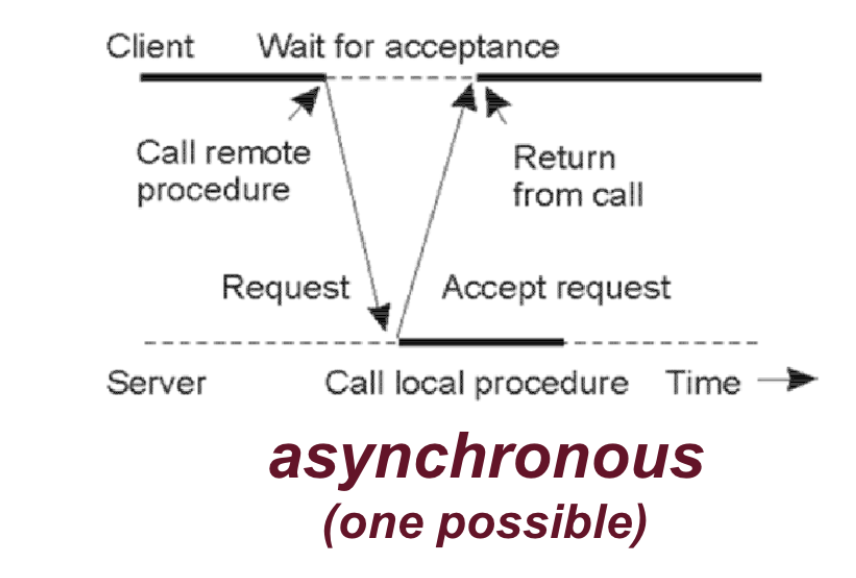
\includegraphics[width=.9\linewidth]{images/async.png}
  \label{fig:async}
\end{minipage}%
\begin{minipage}{.3\textwidth}
  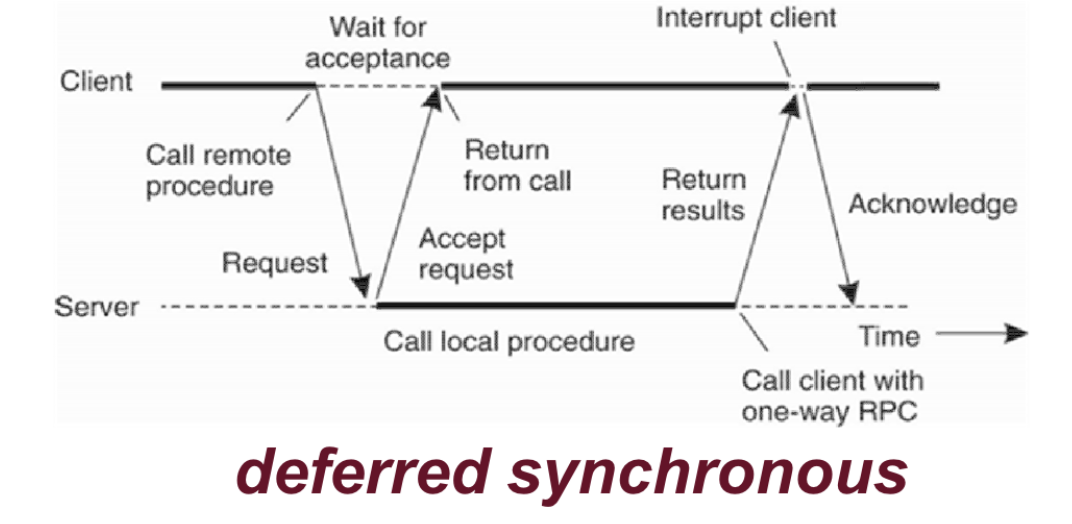
\includegraphics[width=.9\linewidth]{images/def-sync.png}
  \label{fig:def-sync}
\end{minipage}
\end{figure} 
If we have an asynchronous invocation, we don't care if the function (service) is executed immediately or later. The middleware so can optimize the communication over the network by \textbf{buffering} function invocations and then send later them all together. \\
Sun RPC includes the ability to perform \textit{batched} RPC:
\begin{itemize}
	\item RPCs that do not require a result are buffered on the client
	\item They are sent all together when a non-batched call is requested (or when a timeout expires)
	\item Enables yet another form of asynchronous RPC
\end{itemize}
A similar concept can be used to deal with mobility (as in the Rover toolkit by MIT):
\begin{itemize}
	\item If a mobile host is disconnected between sending the request and receiving the reply, the server periodically tries to contact the mobile host and deliver the reply.
	\item Requests and replies can come through different channels
	\item Depending on network conditions and application requirements, the network scheduler module may decide to:
	\begin{itemize}
		\item Send requests in batches
		\item Compress the data
		\item Reorder requests and replies in a non-FIFO order, e.g., to suit application-specified priorities
	\end{itemize}
	\item Promises are used at the client
\end{itemize}
\subsection{Remote method invocation}
\subsubsection{Fundamentals}
\textbf{Remote method invocation (RMI)} is the same idea as RPC, but using different programming constructs. The aim is to obtain the advantages of OOP also in the distributed setting. RMI shares many of the core concepts and mechanisms with RPC. The most important difference of RMI w.r.t. RPC is that remote object references can be passed around. We are managing objects and methods instead of procedures and data structures. \\ In RMI becomes relatively easy to pass object by reference because we are passing something that acts as an object. When we access an object we don't access the attributes of the object, but we use methods. Those method can be changed such that when we invoke the method, it contacts back the object on the source machine to get the requested information. \\
In RPC, the IDL separates the interface from the implementation to handle platform/language heterogeneity. Such separation is one of the basic OO principles. It becomes natural to place the object interface on one host, and the implementation on another. The IDLs for distributed objects are much richer: inheritance, exception handling...
 \begin{figure}[h!]
 \hfill 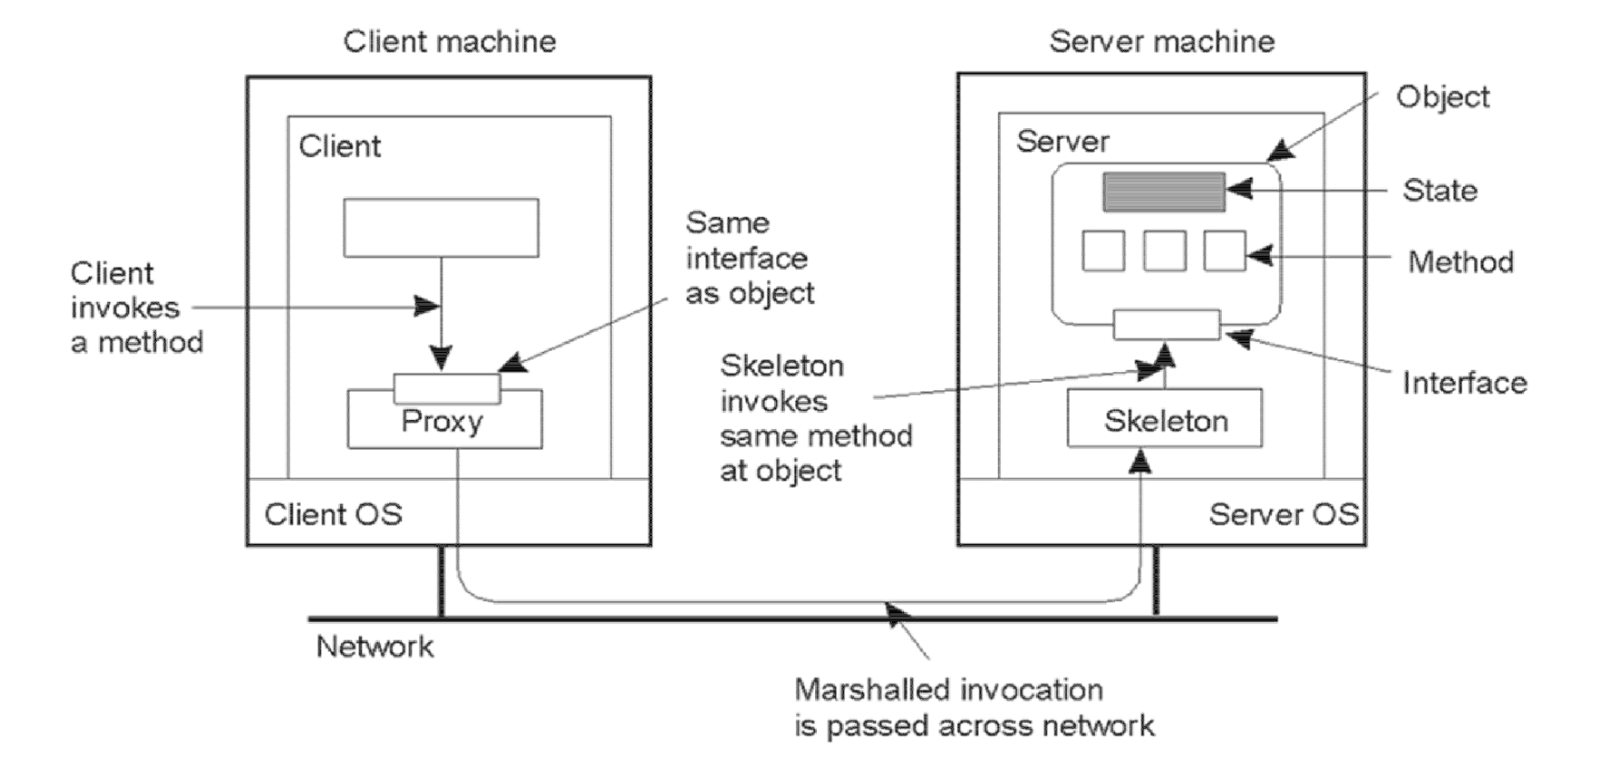
\includegraphics[width=250pt]{images/rmi.png}\hspace*{\fill}
 \caption{RMI client-server architecture}
  \label{fig:rmi}
\end{figure} \\
In general with RMI we cannot pass by copy because it would mean to pass the code and assume that everything is homogeneous (machines may use different languages).\\ \textbf{Java RMI}:
\begin{itemize}
	\item Single language/platform (Java and the Java Virtual Machine)
	\item Easily supports passing parameters by reference or "by value" even in case of complex objects.
	\item Supports for downloading code (code on demand)
\end{itemize}
\textbf{OMG CORBA}:
\begin{itemize}
	\item Multilanguage/multiplaform
	\item Supports passing parameters by reference or by value
	\begin{itemize}
		\item If objects are passed by value (valuetype) it is up to the programmer to guarantee the same semantics for methods on the sender and receiver sides
	\end{itemize}
\end{itemize}
\subsection{Message oriented communication}
\subsubsection{Fundamentals}
RPC and RMI foster a synchronous model and a natural programming abstraction but:
\begin{itemize}
	\item Supports only point-to-point interaction
	\item Synchronous communication is expensive
	\item Intrisically tight coupling between caller and callee, leads to "rigid" architectures
\end{itemize}
\textbf{Message oriented communication}:
\begin{itemize}
	\item Centered around the (simpler) notion of one-way message/event
	\item Usually asynchronous (several forms)
	\item Often supporting persistent communication and multi-point interaction
	\item Brings more decoupling among components
\end{itemize}
There are different types of communication that combined together can generate several alternatives in practice:
\begin{itemize}
	\item Synchronous vs. Asynchronous
	\begin{itemize}
		\item Synchronous: the sender is blocked until the recipient has stored (or received, or processed) the message
		\item Asynchronous: the sender continues immediately after sending the message
	\end{itemize}
	\item Transient vs. Persistent
	\begin{itemize}
		\item Transient: sender and receiver must both be running for the message to be delivered
		\item Persistent: the message is stored in the communication system until it can be delivered
	\end{itemize}
\end{itemize}
\subparagraph{Transient communication}
\begin{itemize}
	\item Asynchronous: client sends a message and continues; communication only happens if the server is running.
	\item Synchronous: 
	\begin{itemize}
		\item Receipt-based: client sends a message and waits until it is received received, and eventually starts processing it later.
	\item Delivery-based: client sends a message and waits until it is accepted (started processing
	\item Response-based: client sends a message and waits until it is processed; 
	\end{itemize}
\end{itemize}
\subparagraph{Persistent communication}
\begin{itemize}
	\item Asynchronous: client sends a message and continues; server may also not be running at that specific time.
	\item Synchronous: client sends a message (that will be stored for later delivery) and waits that it is accepted; later on server processes it.
\end{itemize}
\begin{figure}
	\begin{subfigure}{.9\textwidth}
 \hfill 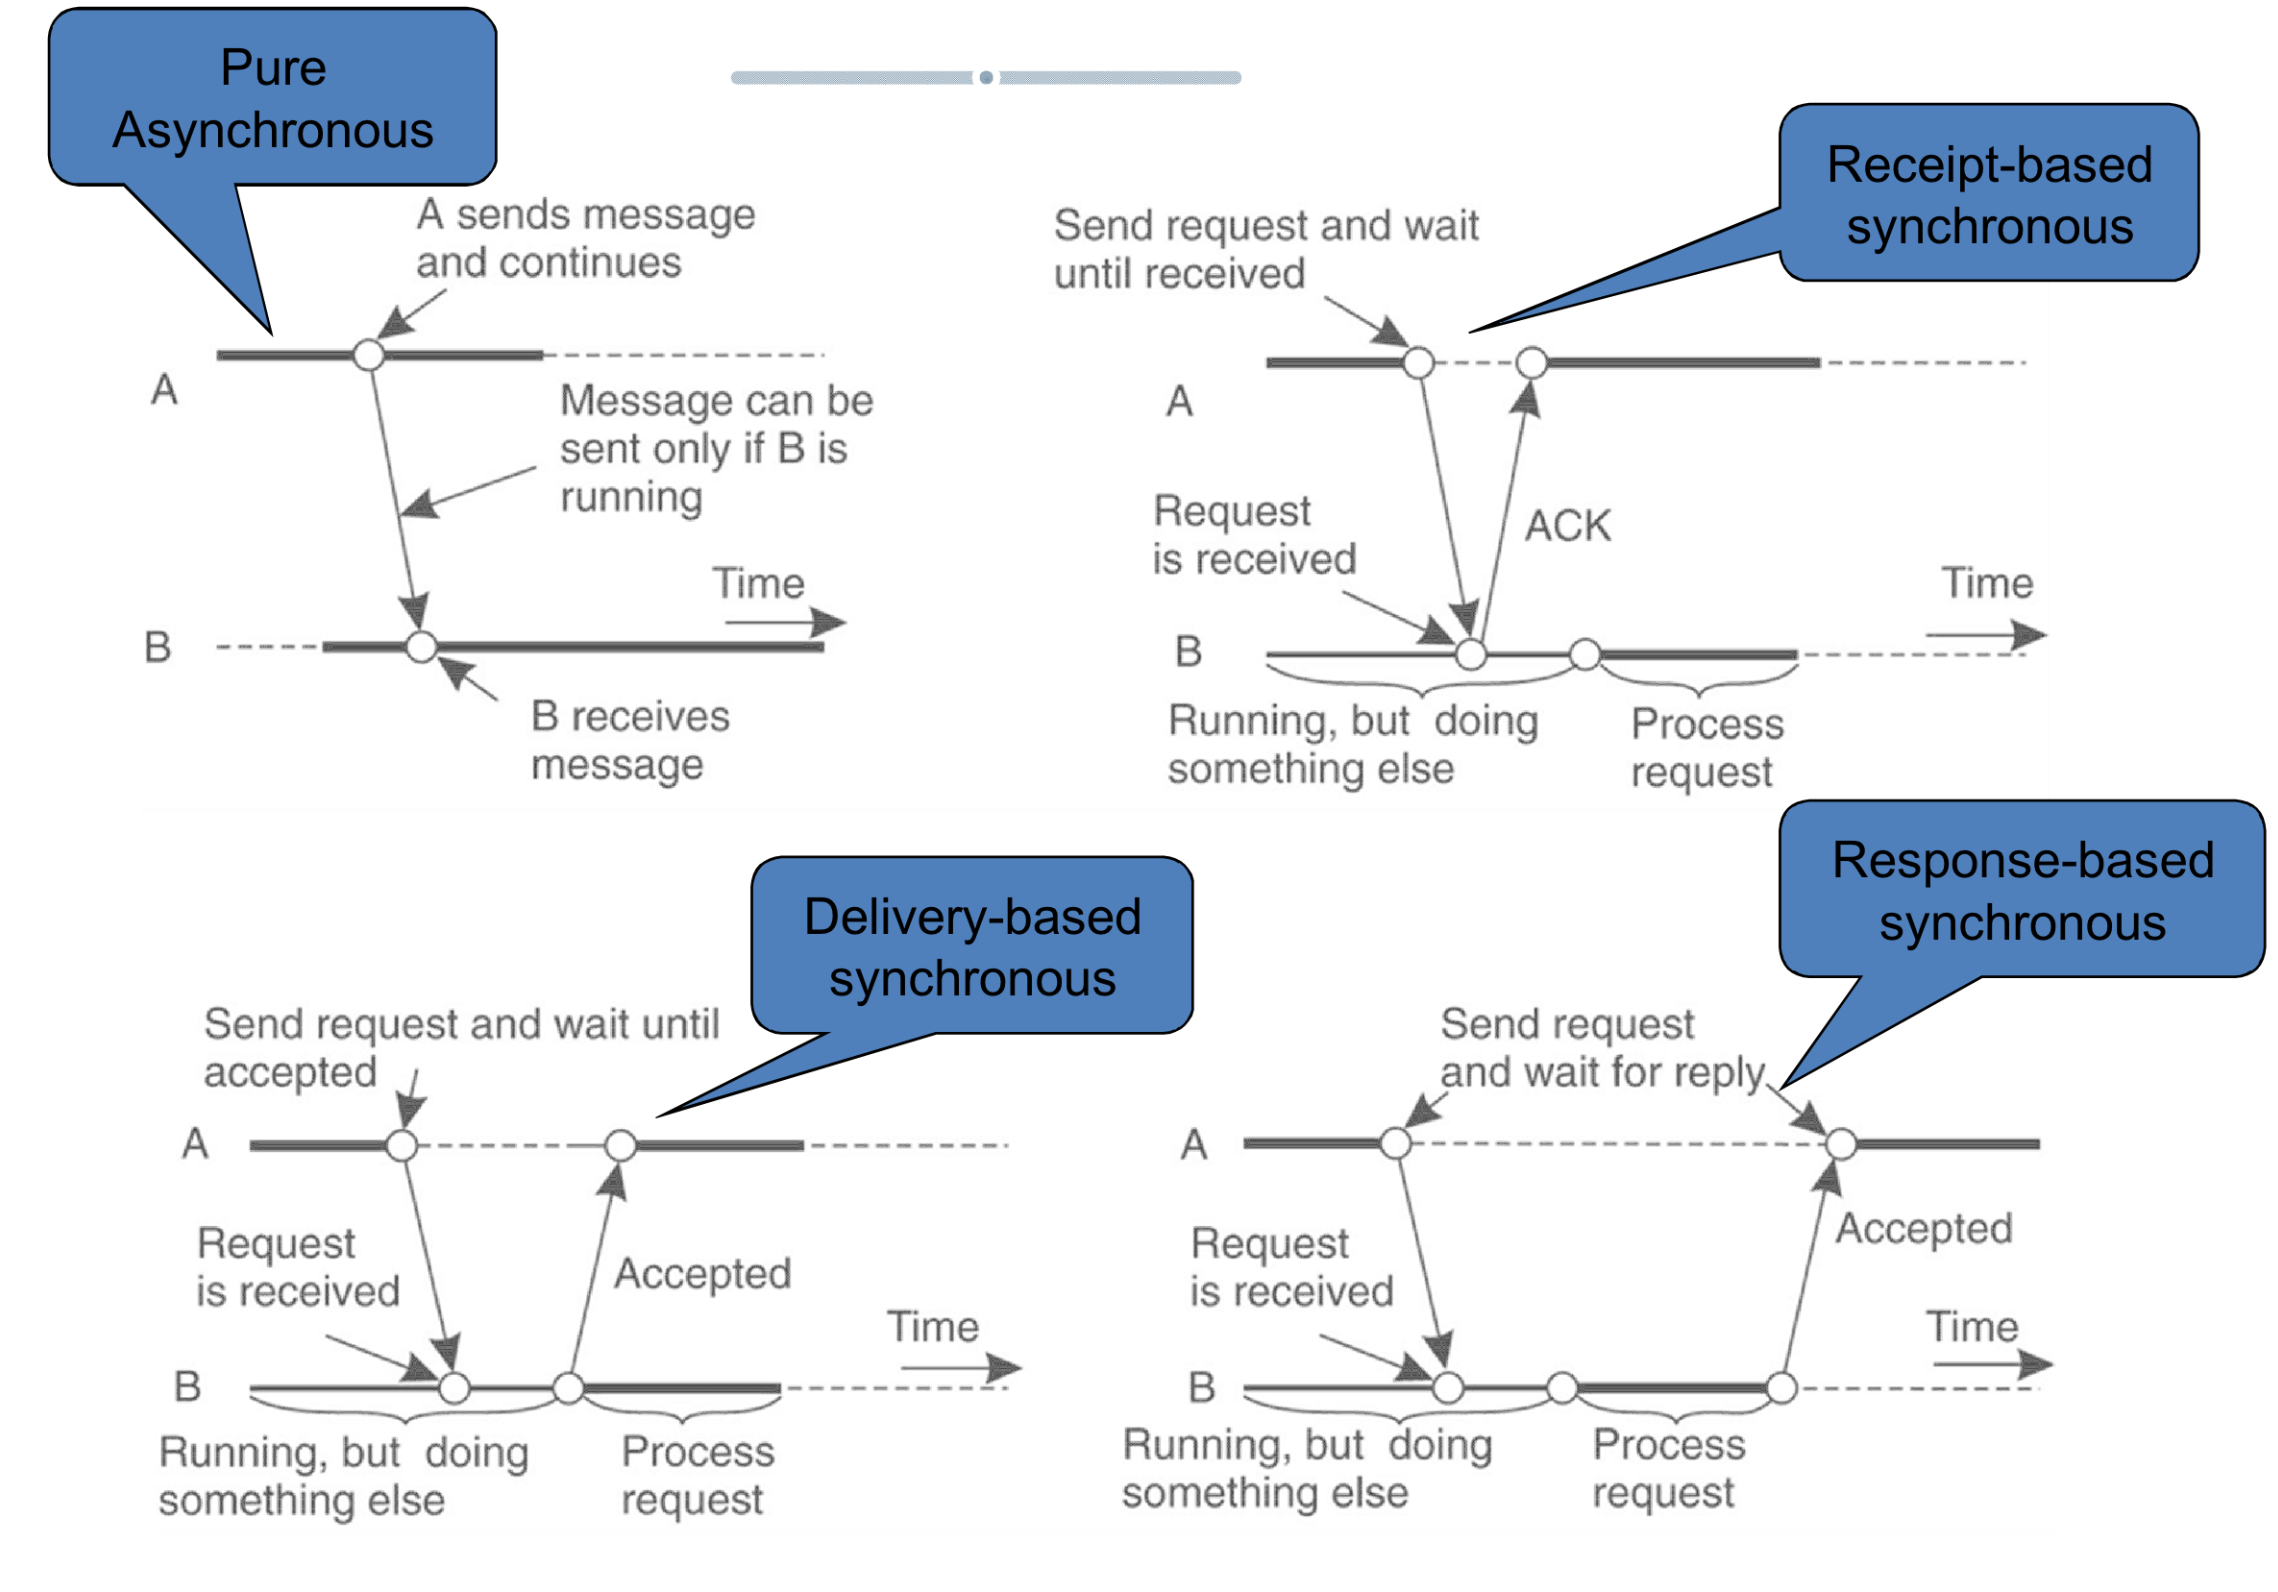
\includegraphics[width=400pt]{images/transient.png}\hspace*{\fill}
 \caption{Transient communication}
  \label{fig:transient}
	\end{subfigure} \\
\\ \\ \\ \\ \\ \\ \\ \\ \begin{subfigure}{.9\textwidth}
 \hfill 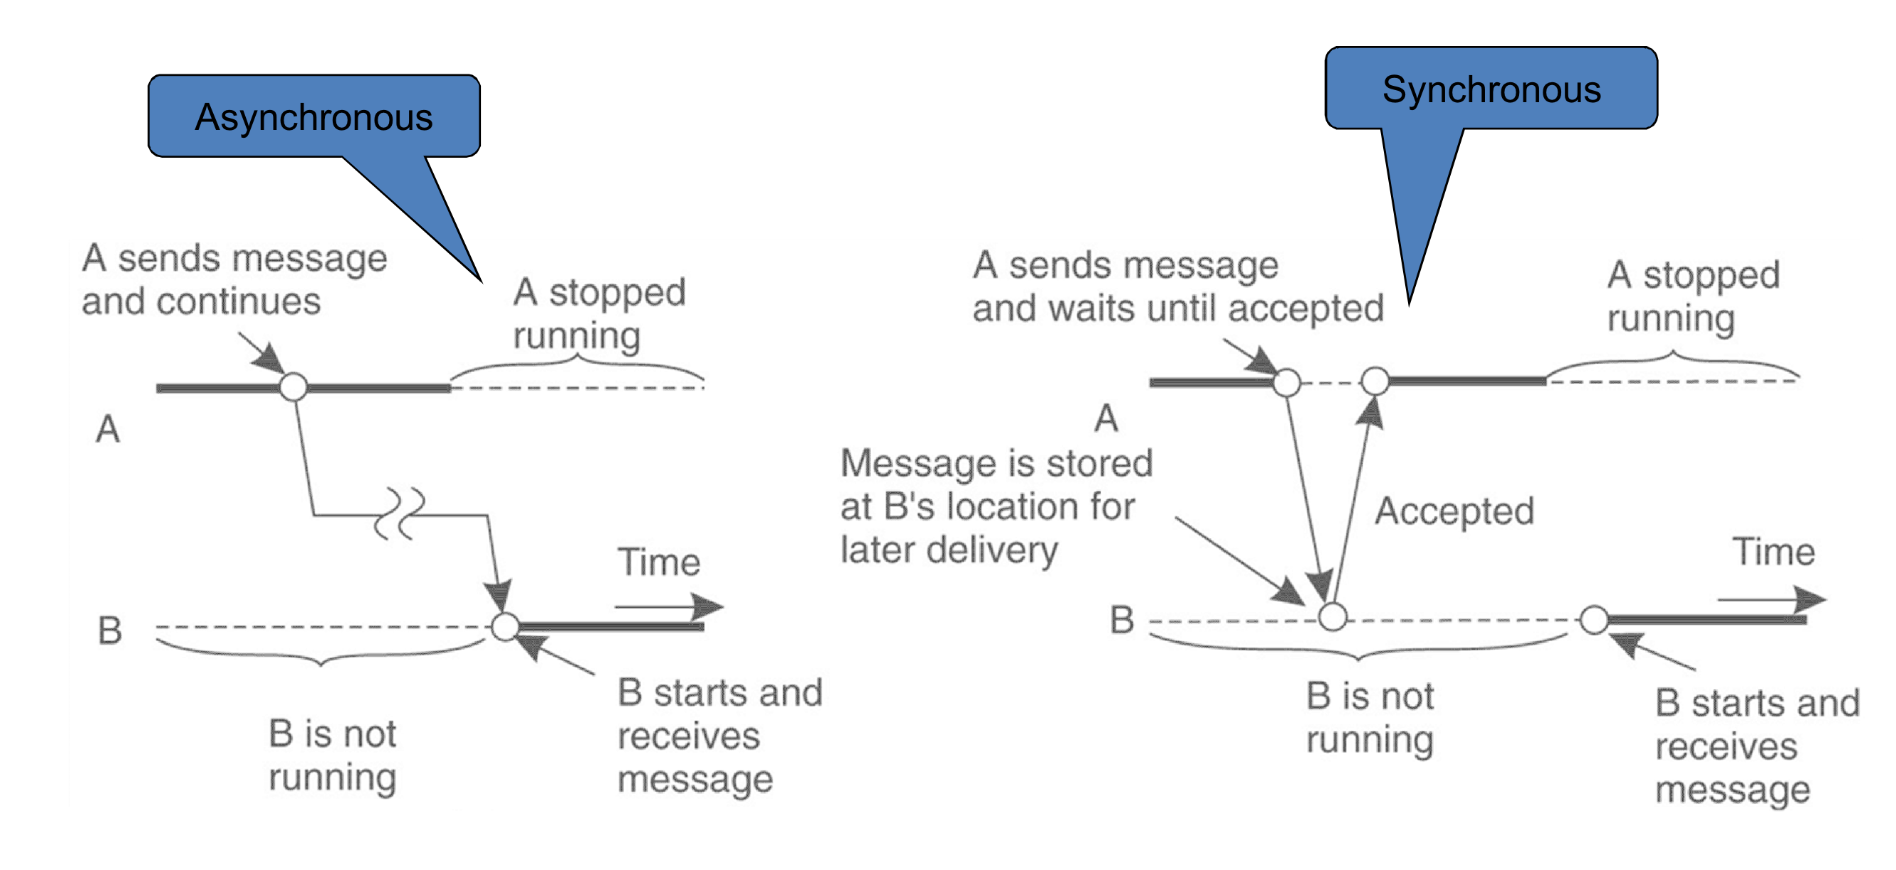
\includegraphics[width=400pt]{images/persistent.png}\hspace*{\fill}
  \caption{Persistent communication}
  \label{fig:persistent}
	\end{subfigure}
\end{figure} \pagebreak 
\subsubsection{Message passing (sockets and MPI)}
The most straightforward form of message oriented communication is \textit{message passing}. Typically it is directly mapped on/provided by the underlying network OS functionality (e.g., \textbf{sockets}). A (kind of) middleware provides another form of message passing called \textbf{MPI} \\
\textit{Message queueing} and \textit{publish/subscribe} are two different models provided at the middleware layer by several "communication servers" through what is nowadays called an \textit{overlay network}
 \begin{figure}[h!]
 \hfill 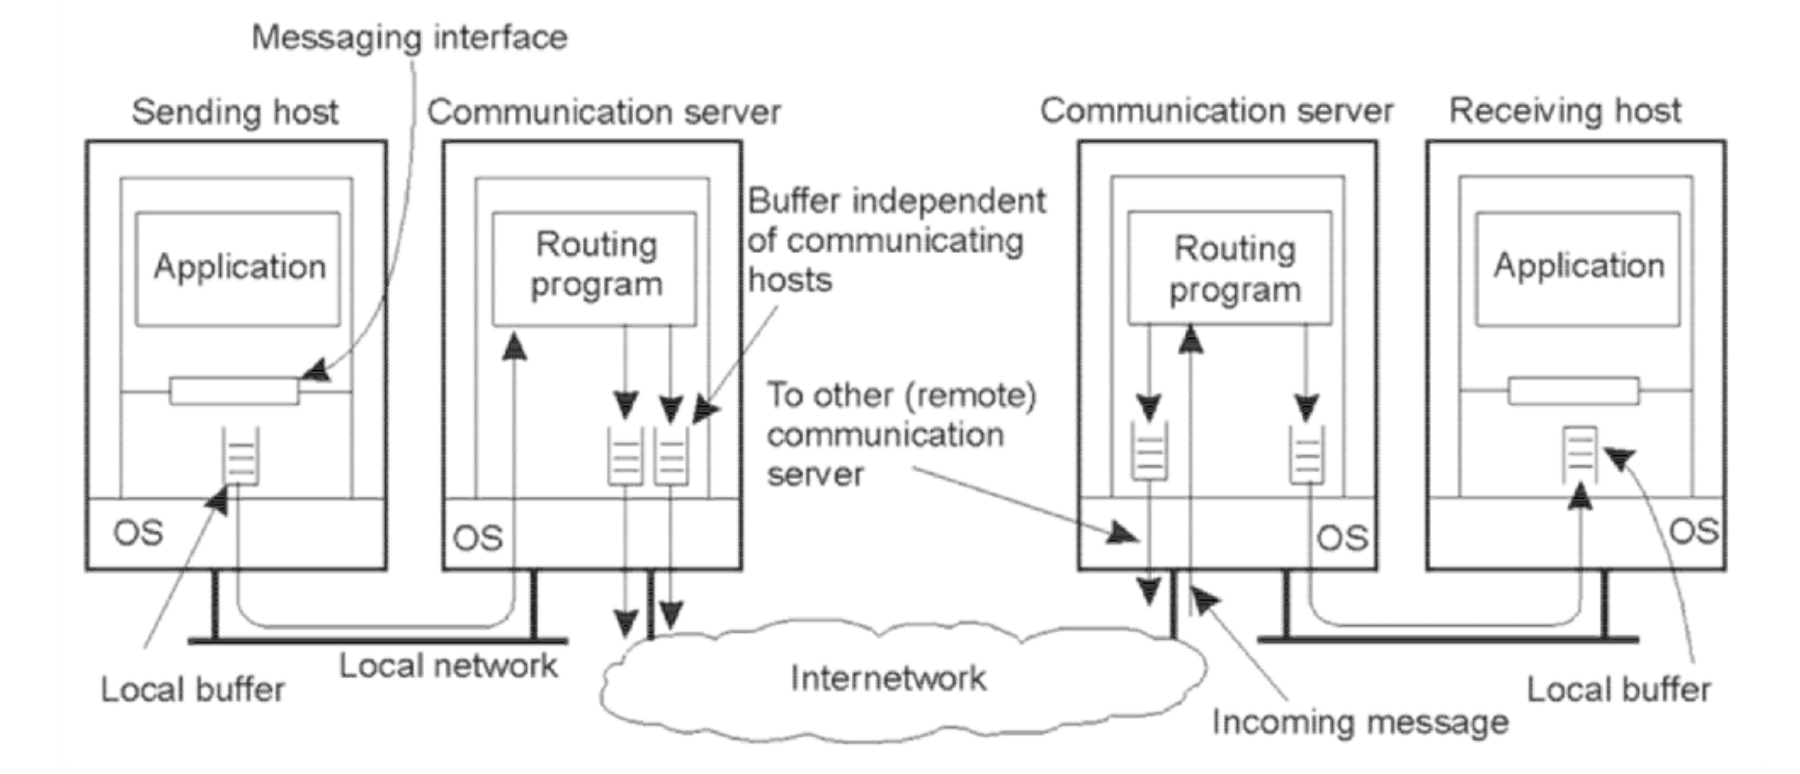
\includegraphics[width=220pt]{images/message-model.png}\hspace*{\fill}
 \caption{Message passing architecture}
  \label{fig:message-model}
\end{figure}
\paragraph{Sockets}
Unicast TCP and UDP (and multicast IP) are well know network protocols, but how a poor programmer can take advantage of such protocols? \textit{Berkeley sockets} are the answer. \\ 
Sockets provide a common abstraction for inter-process communication and allow for connection-oriented (stream i.e., TCP) or connectionless (datagram i.e., UDP) communication.
\subparagraph{Stream sockets}
The server accepts connection on a port. The client connects to the server. Each (connected) socket is uniquely identified by 4 numbers:
\begin{itemize}
	\item IP Address of the server
	\item Server's 'incoming' port
	\item IP Address of the client
	\item Client's 'outgoing' port
\end{itemize}
\subparagraph{Datagram sockets}
Client and server use the same approach to send and receive datagrams: both create a socket bound to a port and use it to send and receives datagrams. There is no connection and the same socket can be used to send (receive) datagrams to (from) multiple hosts. Here, instead of opening a connection and reading/writing block by block, single blocks (datagrams) are sent separated one from another. \\
\begin{figure}[h!]
\centering
\begin{minipage}{.5\textwidth}
  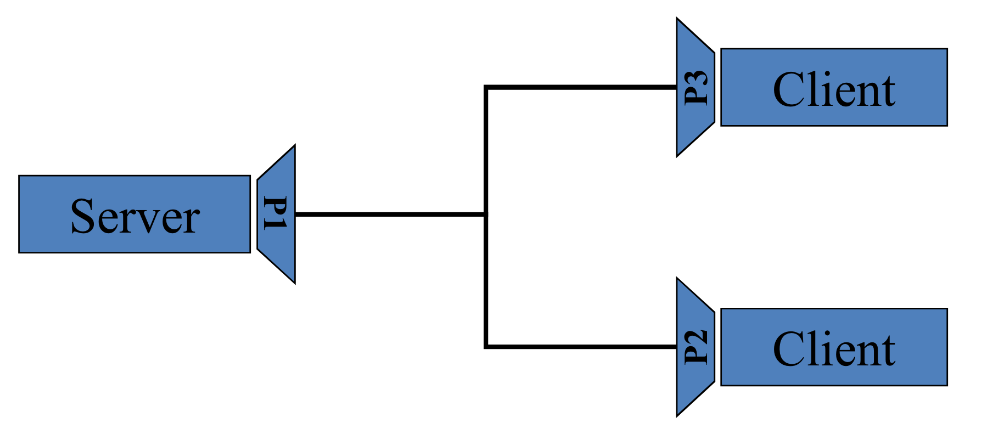
\includegraphics[width=.7\linewidth]{images/stream-sockets.png}
  \caption{Stream sockets}
  \label{fig:stream}
\end{minipage}%
\begin{minipage}{.5\textwidth}
  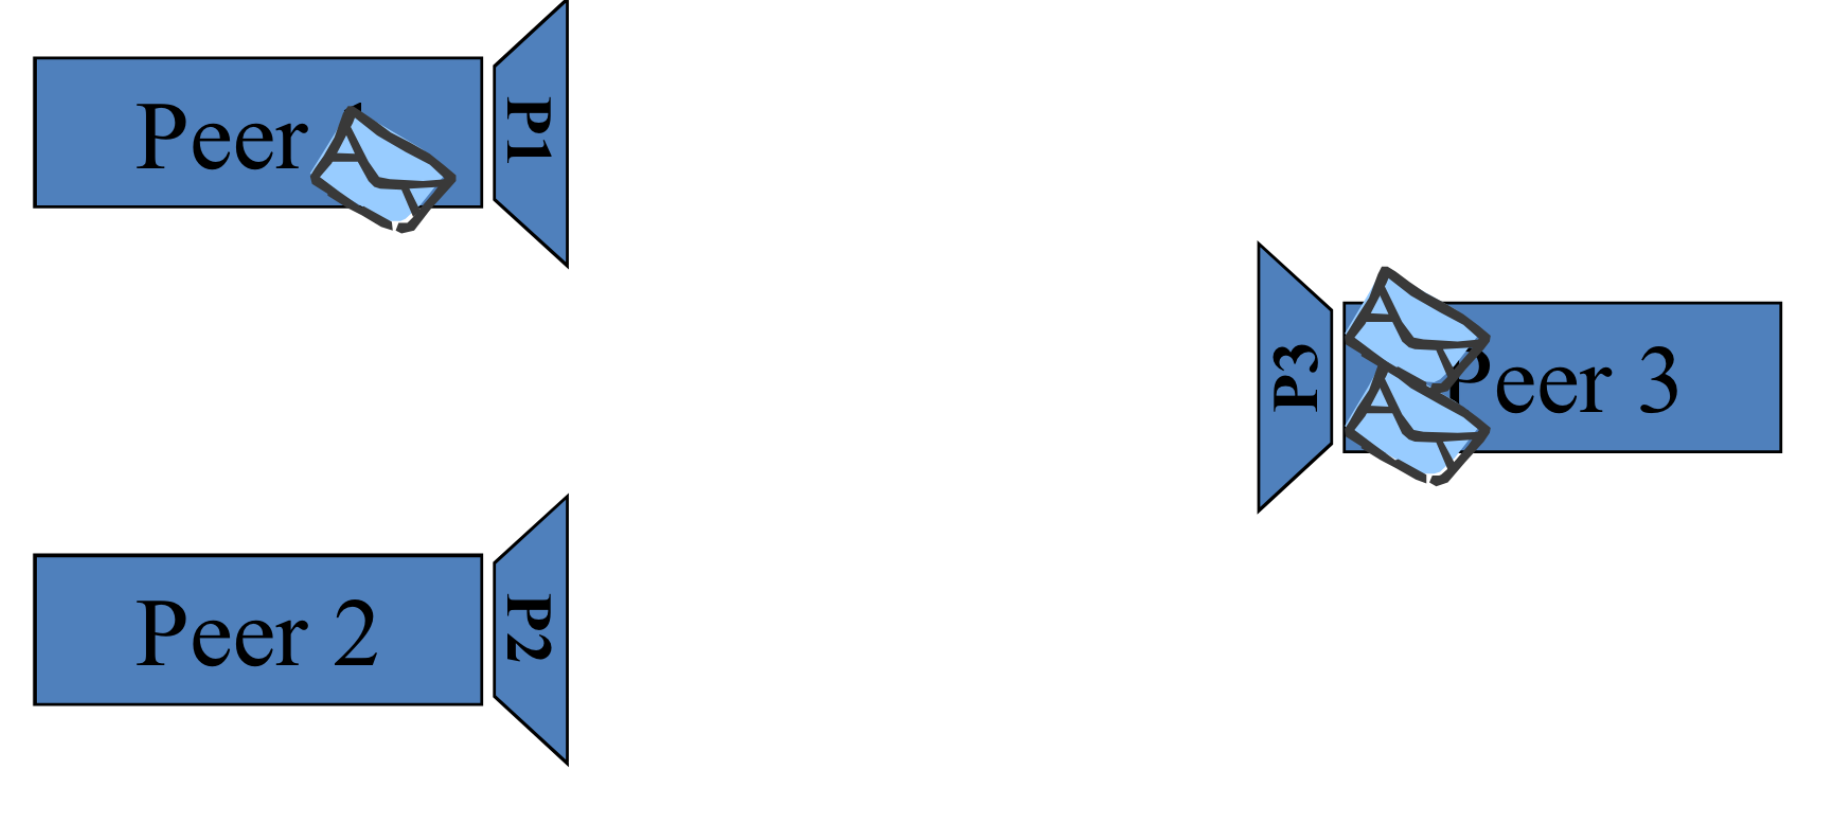
\includegraphics[width=.7\linewidth]{images/datagram-sockets.png}
   \caption{Datagram sockets}
  \label{fig:datagram-sockets}
\end{minipage}
\end{figure} \\
\subparagraph{Multicast sockets}
IP multicast is a network protocol to efficiently deliver UDP datagrams to multiple recipients. The \textit{Internet Protocol} reserves a class D address space, from 224.0.0.0 to 239.255.255.255, to multicast groups. \\
The socket API for multicast communication is similar to that for datagram communication: 
\begin{itemize}
	\item Component interested in receiving multicast datagrams addressed to a specific group must \textit{join} the group.
	\begin{itemize}
		\item Groups are open: it is not necessary to be a member of a group in order to send datagrams to the group
	\end{itemize}
	\item As usual it is also necessary to specify a port, that will be used by the OS to decide which process on the local machine to route packets to
\end{itemize}
In practice, we send the packet to a group and all the nodes connected to the group will receive the packet. Note that most routers are configured to not route multicast packets outside the LAN.
\paragraph{MPI}
Main limitation of sockets:
\begin{itemize}
	\item Low Level
	\item Protocol independent, in sockets we use the same procedures independently on the fact that we are using Streams or Datagrams
\end{itemize}
In high performance networks (e.g., clusters of computers) we need higher level primitives for asynchronous and transient communication, providing different services besides pure read and write. \textbf{MPI} is the platform independent answer. \\ 
In MPI communication takes place withing a known group of processes. 
\begin{itemize}
	\item Each process within a group is assigned a local id.
	\item The pair (groupID, processID) represents a source or destination address.
	\item Messages can also be sent in broadcast to the entire group.
	\item There is no support for fault tolerance
\end{itemize}  
 \begin{figure}[h!]
 \hfill 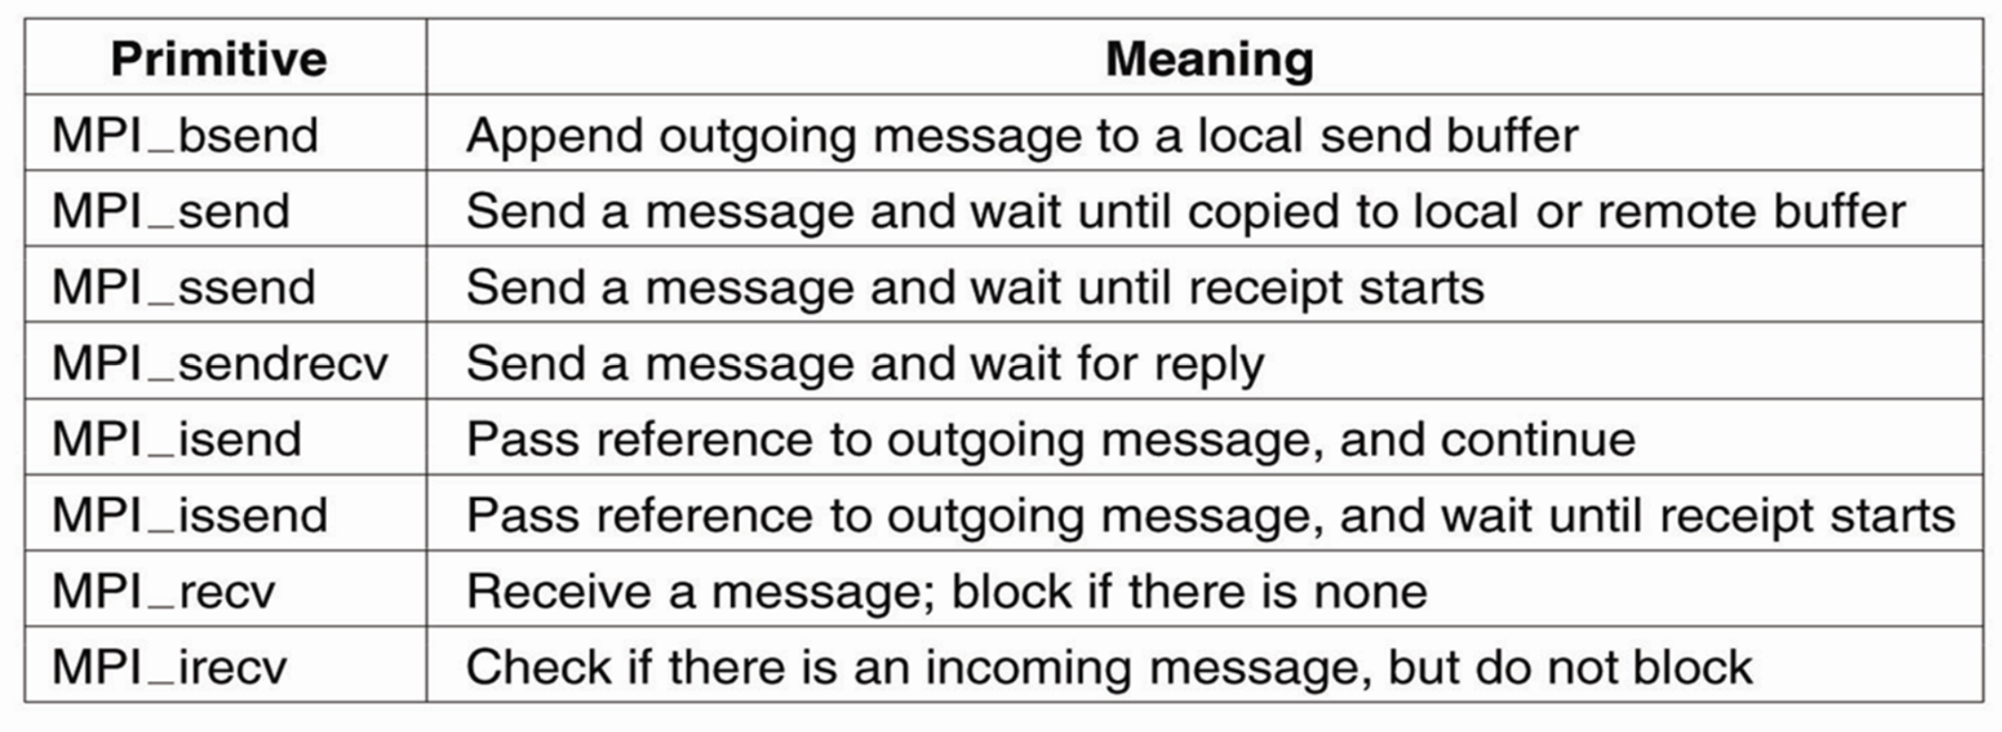
\includegraphics[width=220pt]{images/mpi.png}\hspace*{\fill}
 \caption{Main MPI primitives}
  \label{fig:mpi}
\end{figure}
\subsubsection{Message queueing}
In \textbf{Message queueing} we don't send a message directly to a process like MPI or sockets, but we send a message to a queue. \\
Message queueing is a point-to-point persistent asynchronous communication.
\begin{itemize}
	\item Typically guarantee only eventual insertion of the message in the recipient queue (no guarantee about the recipient's behavior).
	\item The communication is decoupled in time and space.
	\item Can be regarded as a generalization of e-mail
\end{itemize}
 \begin{figure}[h!]
 \hfill 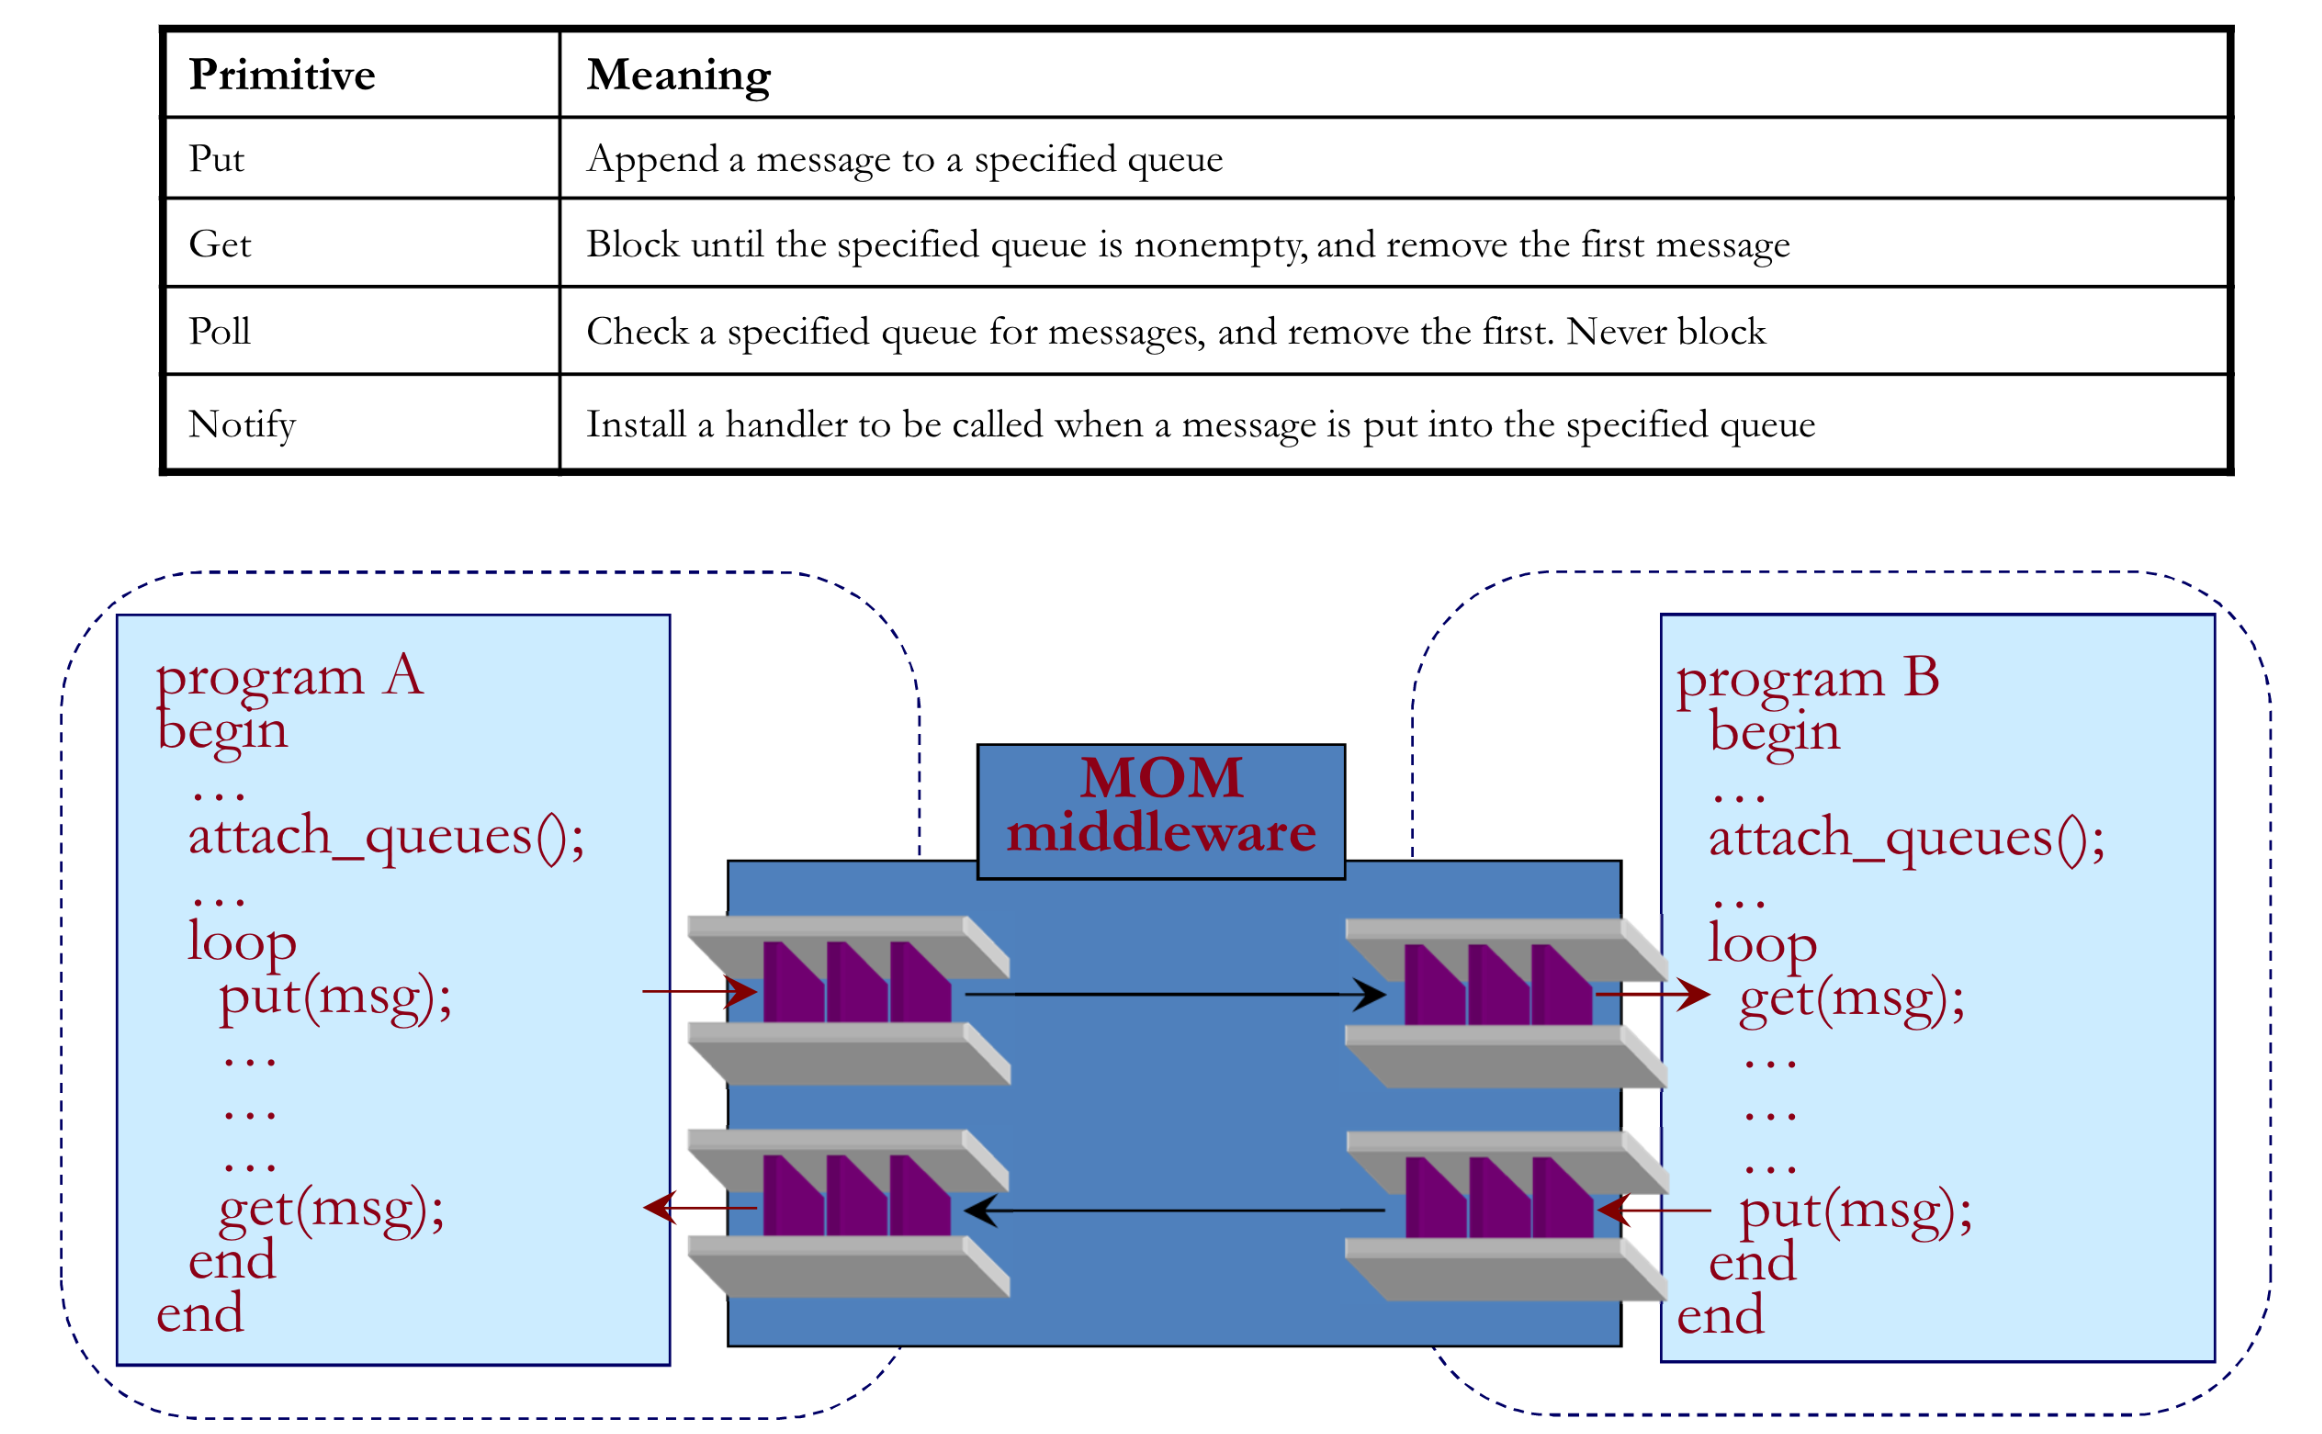
\includegraphics[width=220pt]{images/message-queueing.png}\hspace*{\fill}
 \caption{Message queueing: communication primitives}
  \label{fig:message-queueing}
\end{figure}
Message queueing is intrinsically a peer-to-peer architecture, because each component holds an input queue and an output queue.
Queues decouple sender and receiver. This decoupling adds complexity over the application layer. \\ Clients send requests to the server's queue. The server asynchronously fetches requests, processes them, and returns results in the clients' queue. 
\begin{itemize}
	\item Thanks to persistency and asynchronocity, clients do not need to remain connected
	\item Queue sharing simplifies load balancing
\end{itemize}
 \begin{figure}[h!]
 \hfill 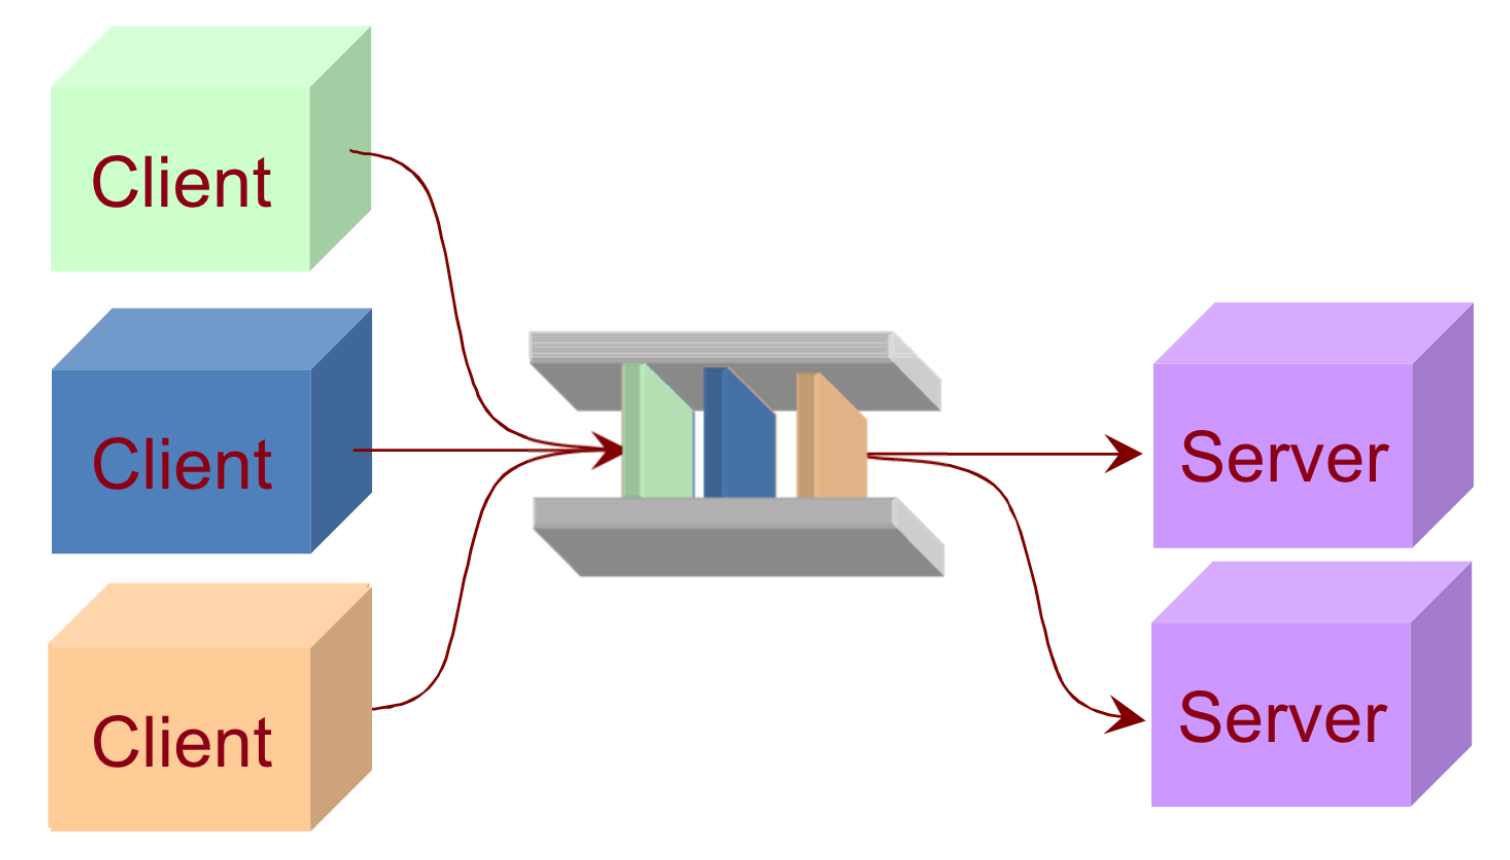
\includegraphics[width=220pt]{images/cs-queue.png}\hspace*{\fill}
 \caption{Client-Server with queues}
  \label{fig:cs-queue}
\end{figure}
\paragraph{Architectural issues}
\subparagraph*{Queues are identified by symbolic names}
Need for a lookup service, possibly distributed, to convert queue-level address in network addresses. Often pre-deployed static topology/naming.
 \begin{figure}[h!]
 \hfill 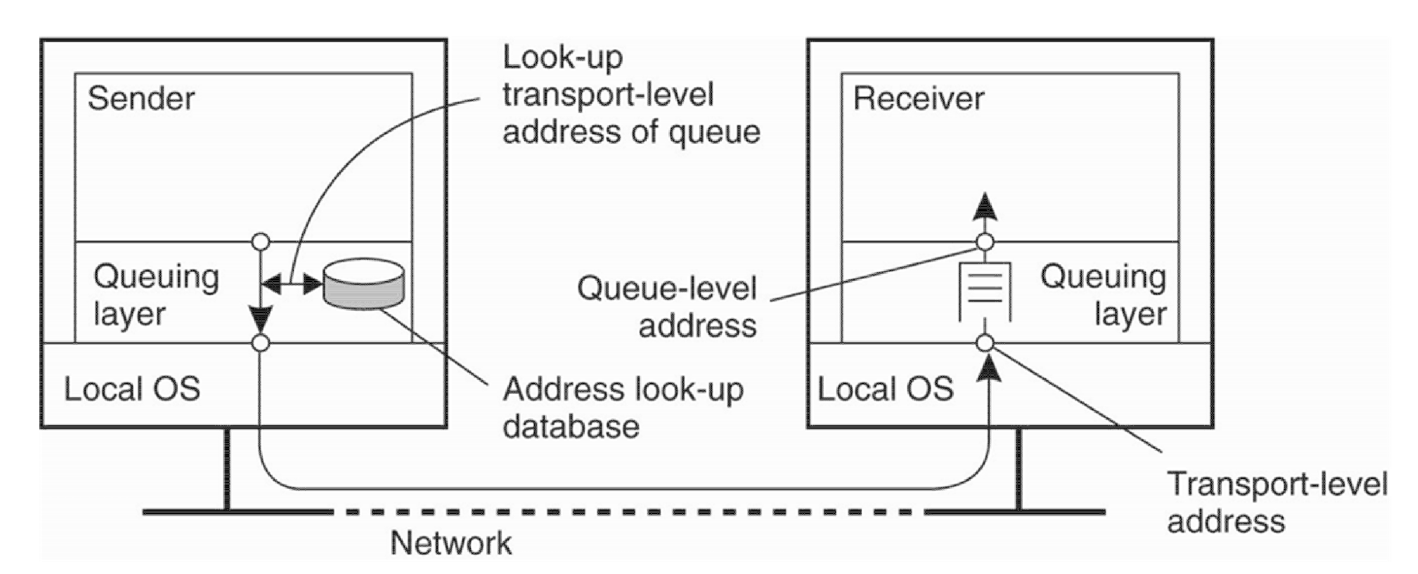
\includegraphics[width=170pt]{images/m-ai1.png}\hspace*{\fill}
  \label{fig:m-ai1}
\end{figure}
\subparagraph{Queues are manipulated by queue managers}
Queue managers are local and/or remote, acting as relays (a.k.a. applicative routers). Relays are often organized in an overlay network. 
\begin{itemize}
	\item Messages are routed by using application-level criteria, and by relying on a partial knowledge of the network
	\item Improves fault tolerance
	\item Provides applications with multi-point without IP-level multicast
\end{itemize}
 \begin{figure}[h!]
 \hfill 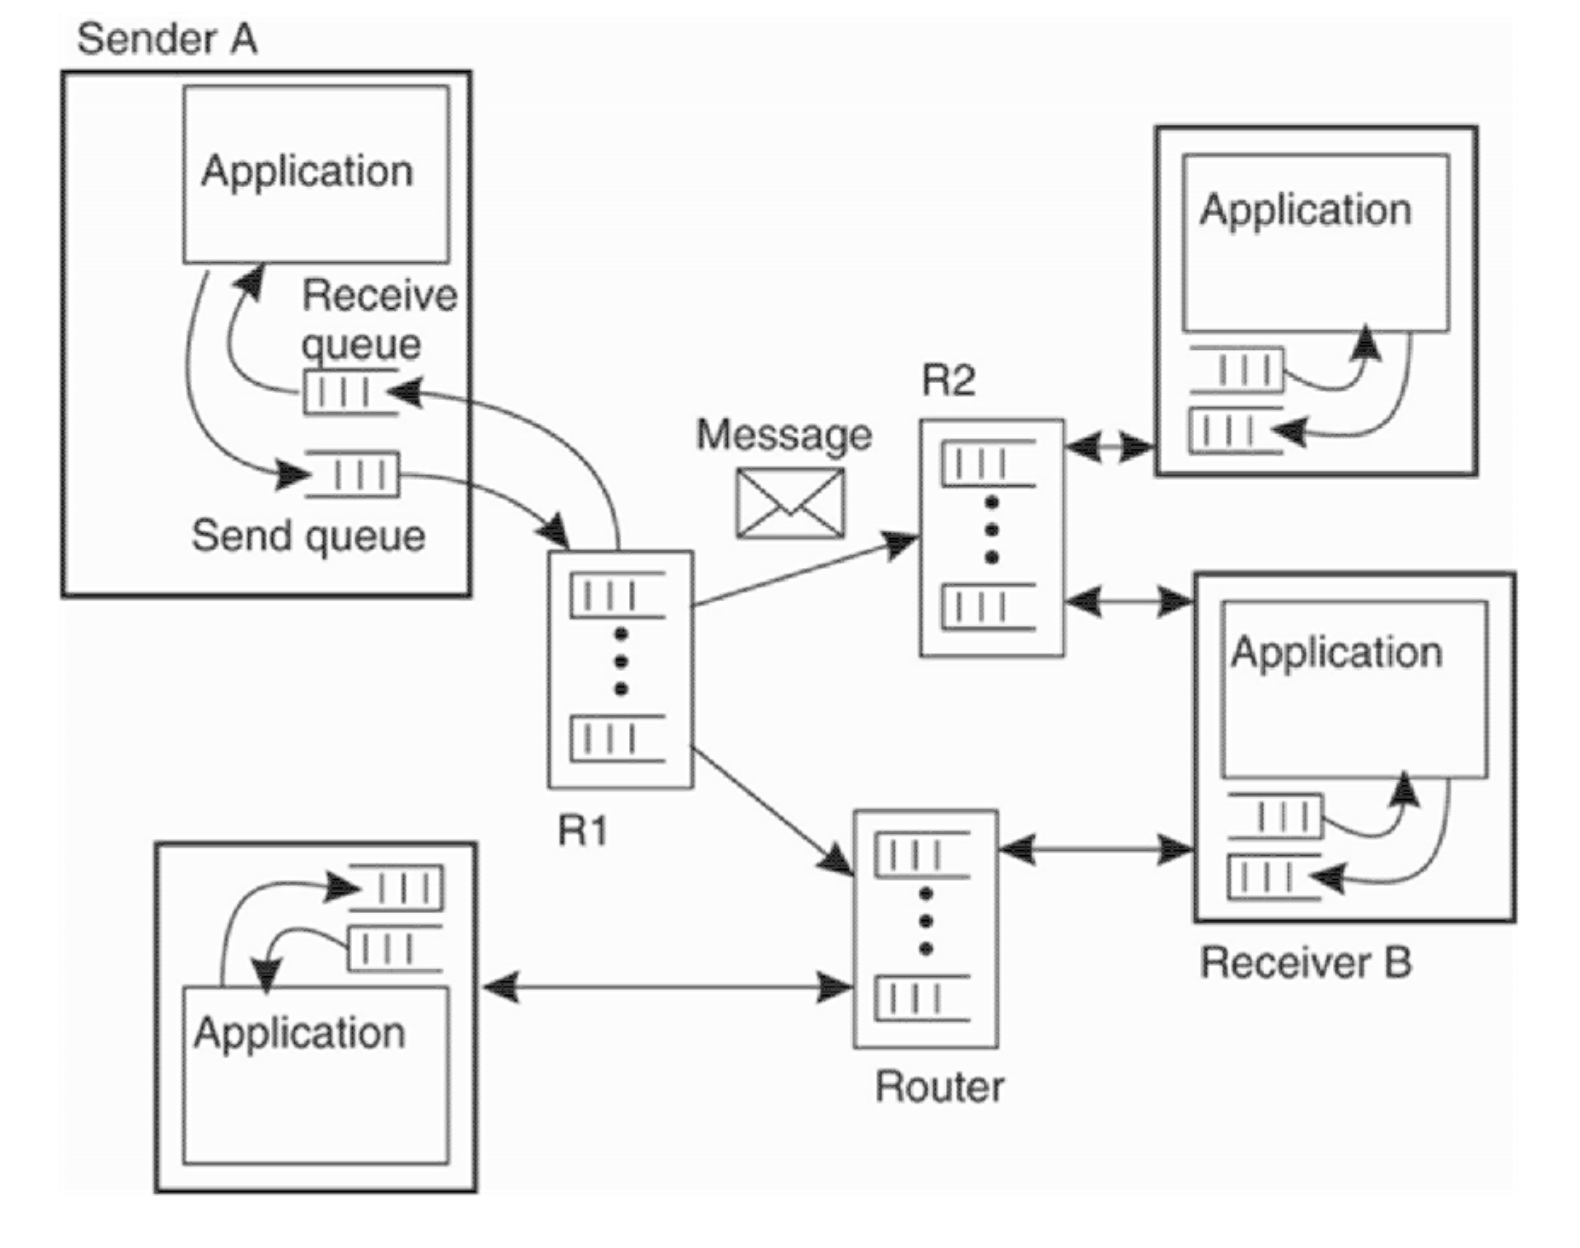
\includegraphics[width=170pt]{images/m-ai2.png}\hspace*{\fill}
  \label{fig:m-ai2}
\end{figure}
\subparagraph{Brokers provide application-level gateways supporting message conversion}
Useful when integrating sub-systems.
 \begin{figure}[h!]
 \hfill 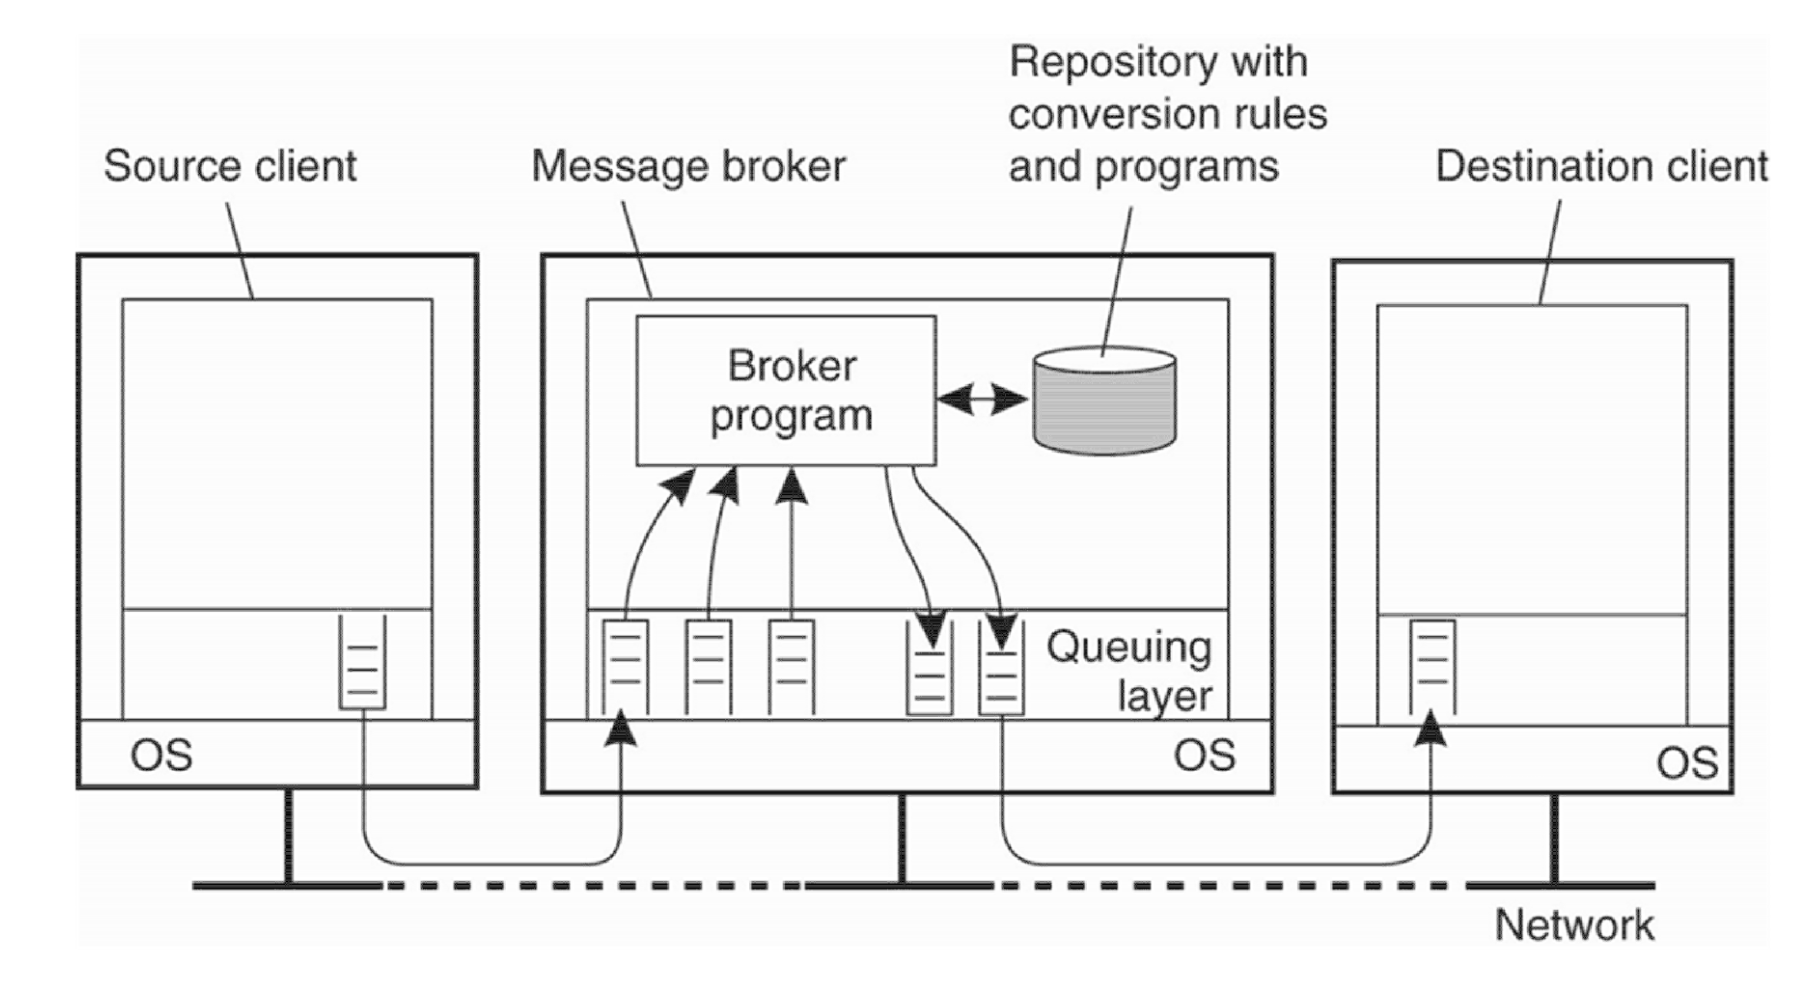
\includegraphics[width=170pt]{images/m-ai3.png}\hspace*{\fill}
  \label{fig:m-ai3}
\end{figure}
\subsubsection{Publish/subscribe}
Application components can \textbf{publish} asynchronous \textit{event notifications}, and/or declare their interest in event classes by issuing a \textbf{subscription}. Event notifications are simply messages. This mechanism uses an extremely simple API composed by only two primitives (publish,subscribe). \\
Subscriptions are collected by an \textit{event dispatcher} component, responsible for routing events to all matching subscribers. The dispatcher can be either centralized or distributed. \\
There is an high degree of decoupling among components: easy to add and remove components (appropriate for dynamic environments). \\
Communication is:
\begin{itemize}
	\item Transiently asynchronous: events are not stored
	\item Implicit: clients get only events that match the subscription
	\item Multipoint: event will reach all the subscribers
\end{itemize}
The expressiveness of the subscription language allows one to distinguish between:
\begin{itemize}
	\item \textit{Subject-based} (or topic-based): 
	\begin{itemize}
		\item The topic is a string that identifies a set of potential notifications in that area
		\item Similar to multicast where clients joined a group and received all the messages of that group
		\item e.g., subscribe to all events about "Distributed Systems".
	\end{itemize}
	\item \textit{Content-based}:
	\begin{itemize}
		\item The subscription may distinguish messages according to their contents
		\item Messages are record with attributes and method
		\item A single event may match multiple subscriptions
		\item e.g., subscribe to all events about "Distributed Systems" class with date greater than 16.11.2004 and held in classroom D04
	\end{itemize}
\end{itemize}
The two can be combined.
Tradeoffs:
\begin{itemize}
	\item Complexity of the implementation vs. expressiveness
	\item However, expressiveness allows additional filtering!
\end{itemize}
In event-based systems a special component of the architecture, the \textit{event dispatcher}, is in charge of collecting subscriptions and routing event notifications based on such subscriptions. For scalability reasons, its implementation can be distributed.
 \begin{figure}[h!]
 \hfill 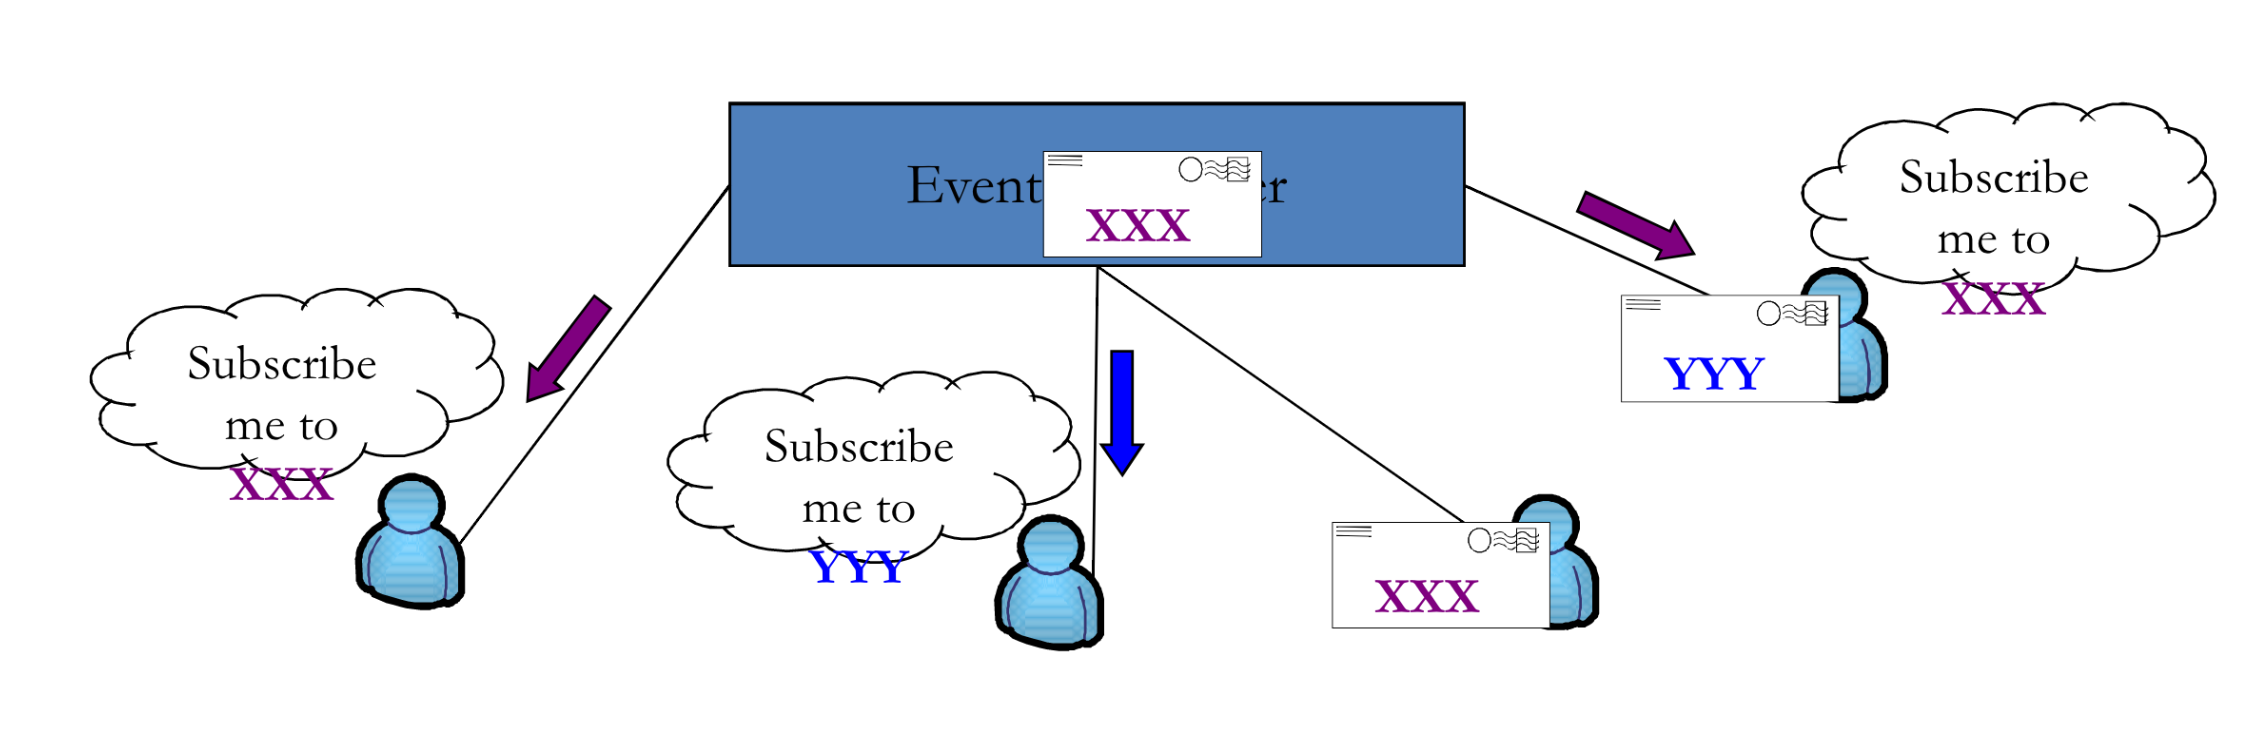
\includegraphics[width=180pt]{images/event-dispatcher.png}\hspace*{\fill}
 \caption{Event dispatcher implementation}
  \label{fig:event-dispatcher}
\end{figure} \\ \\ \\ \\
The architecture of the dispatcher can be either:
\begin{itemize}
	\item \textit{Centralized}: a single component is in charge of collecting subscriptions and forward messages to subscribers
	\item \textit{Distributed}: a set of \textit{message brokers} organized in an \textit{overlay network} cooperate to collect subscriptions and route messages. The topology of the overlay network and the routing strategy adopted may vary (acyclic vs. cyclic overlay).
\end{itemize}
\begin{figure}[h!]
\centering
\begin{minipage}{.5\textwidth}
  \centering
  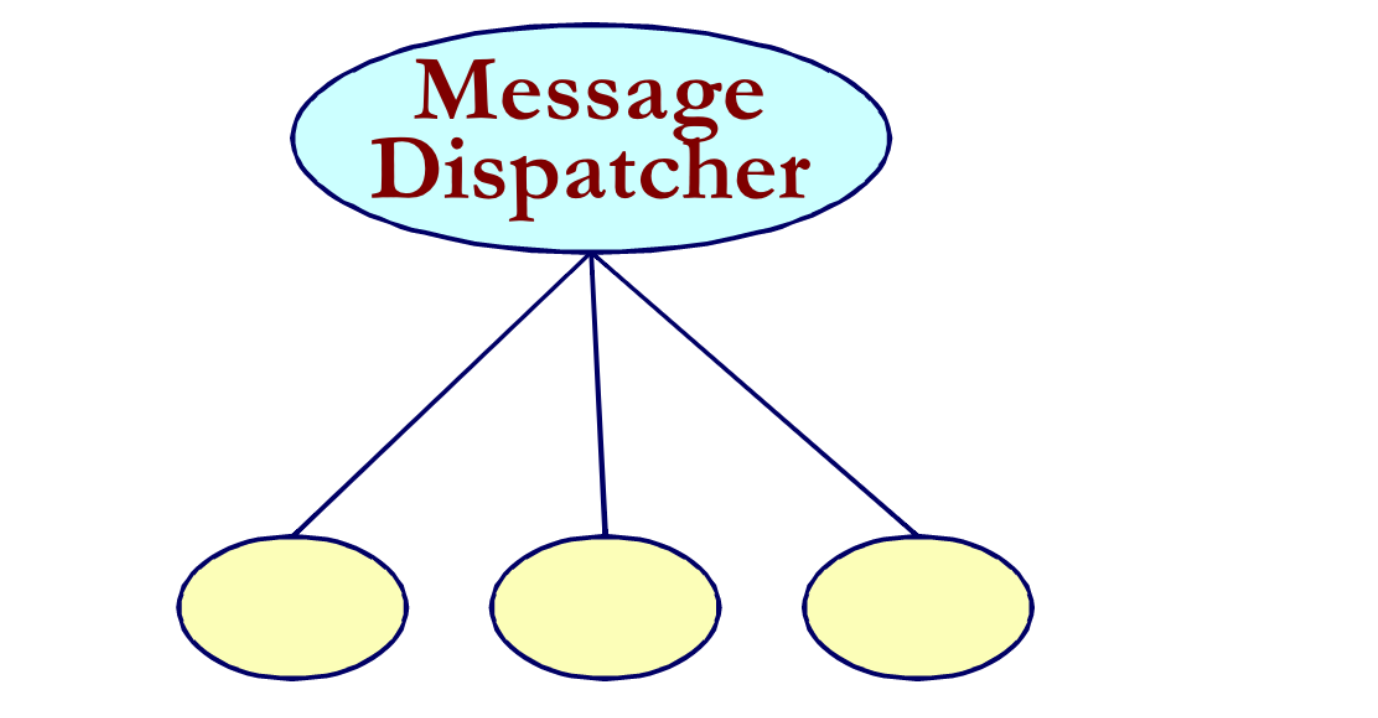
\includegraphics[width=.5\linewidth]{images/dispatcher-cen.png}
  \captionof{figure}{Centralized architecture}
  \label{fig:dispatcher-cen}
\end{minipage}%
\begin{minipage}{.5\textwidth}
  \centering
  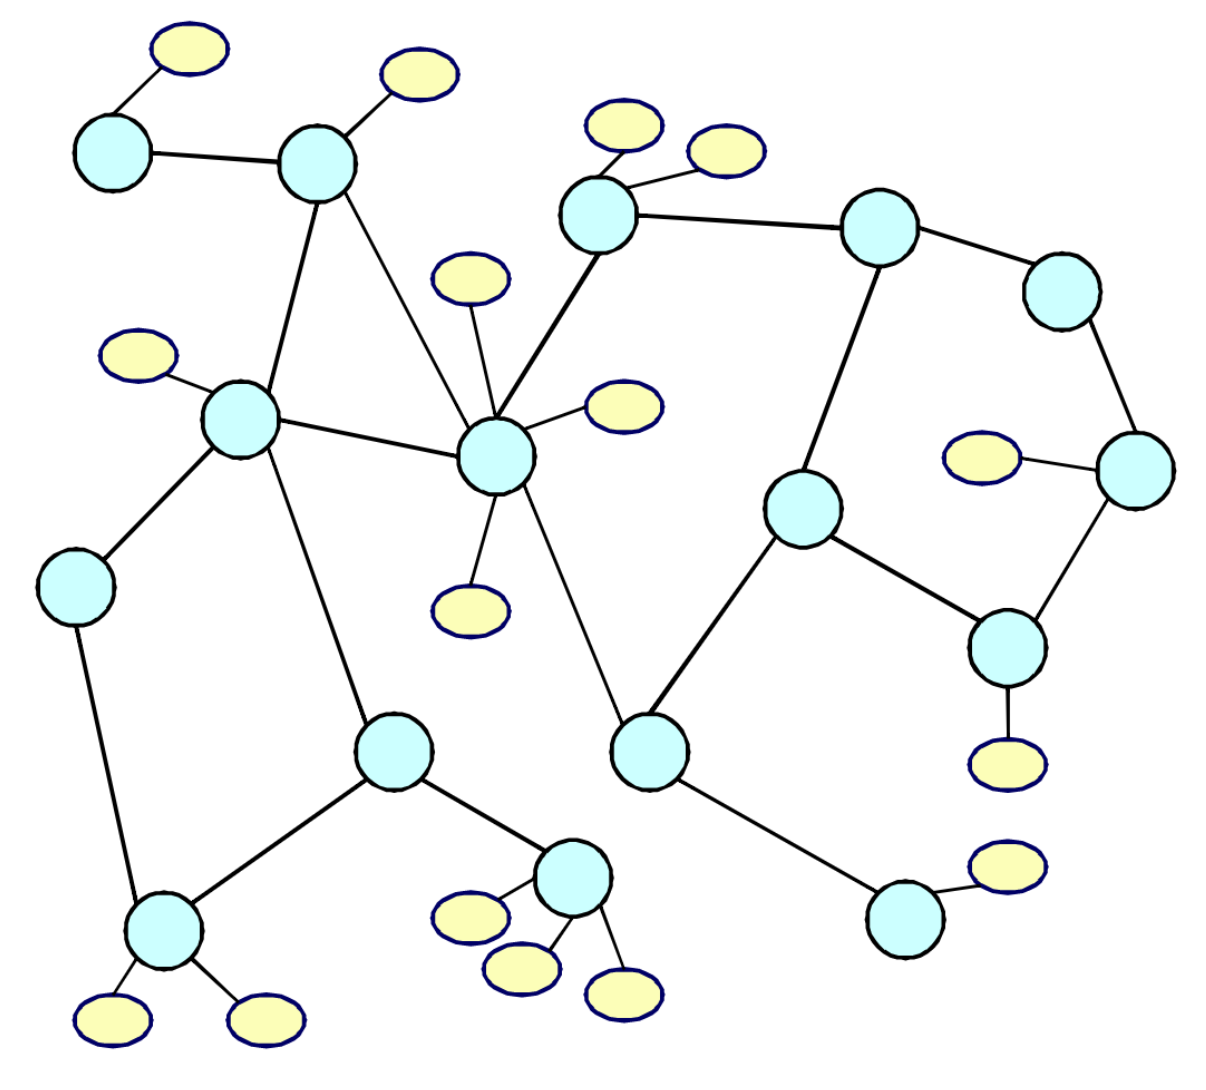
\includegraphics[width=.3\linewidth]{images/dispatcher-dist.png}
  \captionof{figure}{Distributed architecture}
  \label{fig:dist-disp}
\end{minipage}
\end{figure} 
\paragraph{Acyclic topologies}
\subparagraph{Message forwarding} 
Message forwarding consists in taking a message and forward it to all nodes interested. \\
Each broker only store subscription information of the immediately connected component. The message is always forwarded even if the near broker is not subscribed, because along the forwarding path the message can encounter a real subscriber interested in it. The routing table is simple because the number of the subscriptions is small. \\
 \begin{figure}[h!]
 \hfill 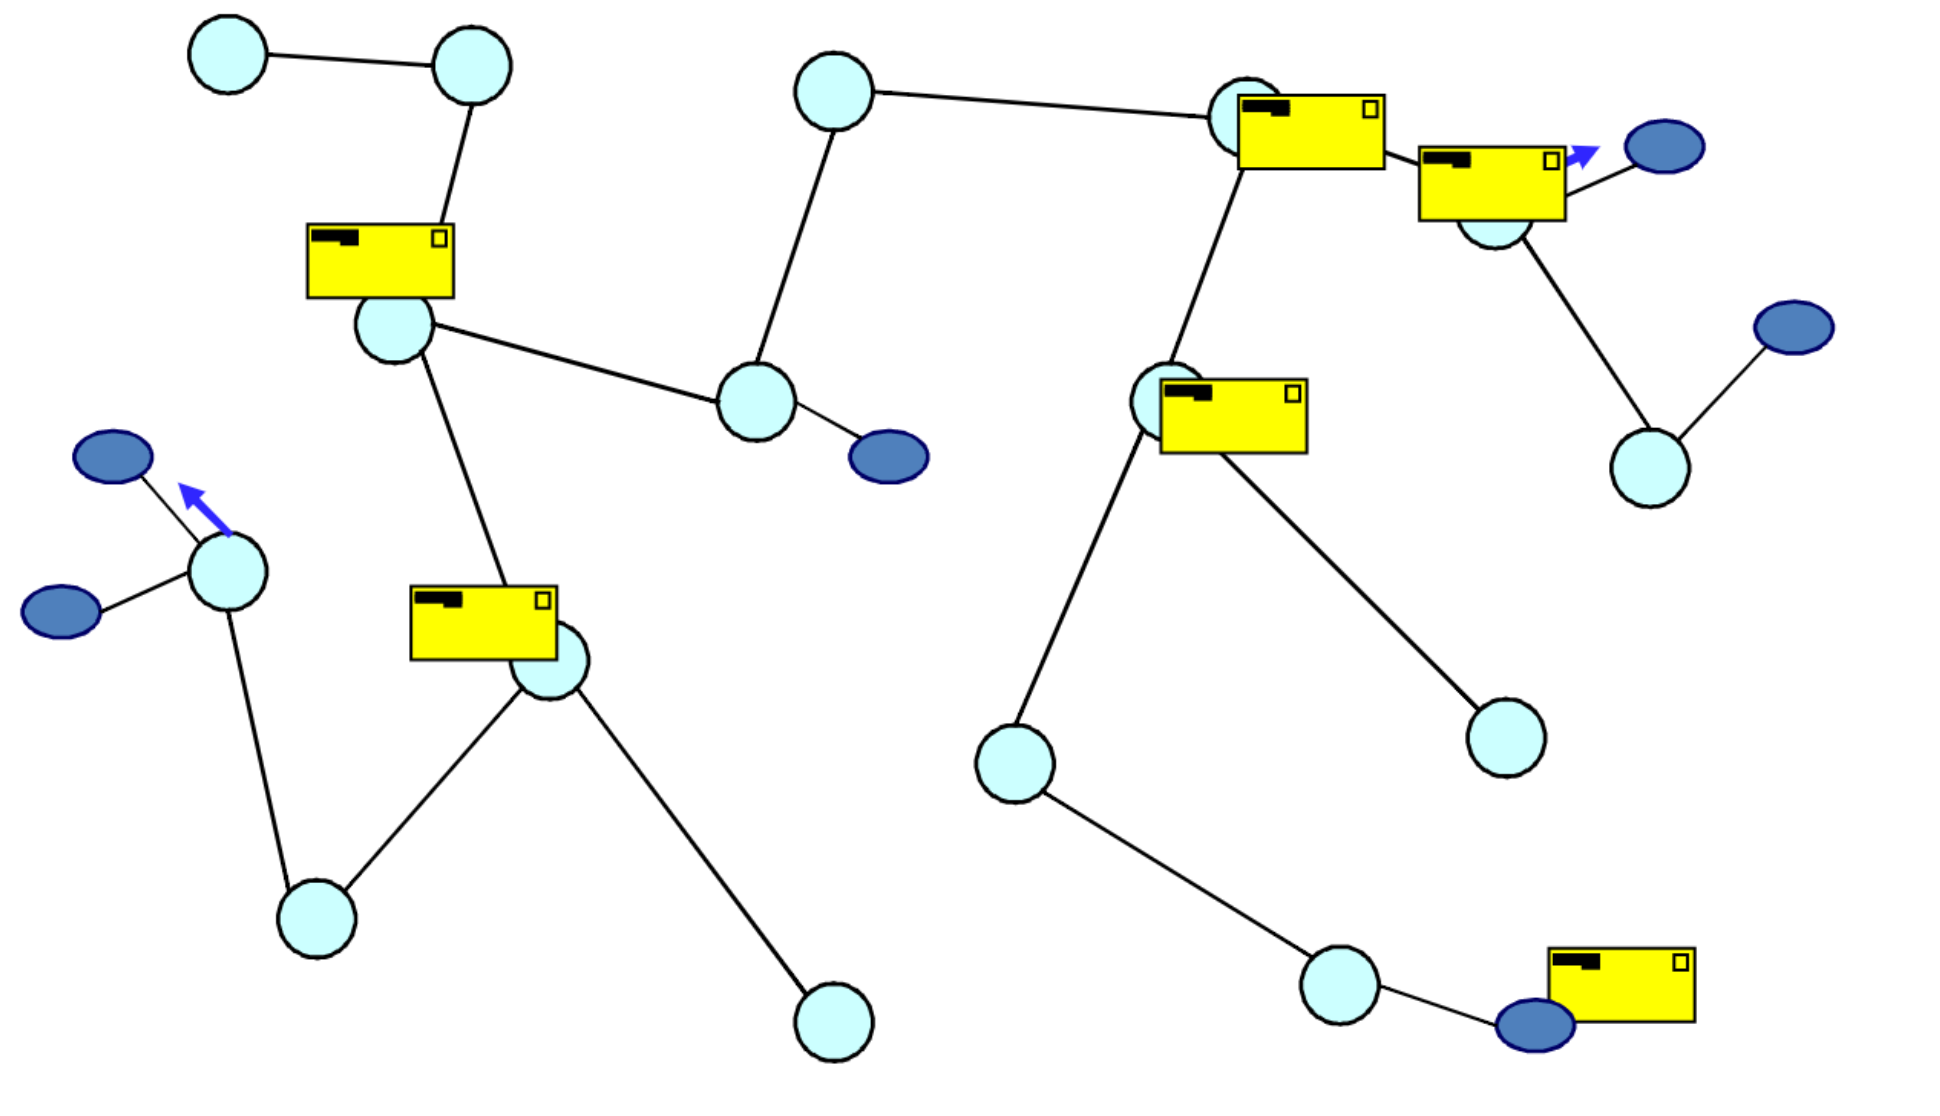
\includegraphics[width=100pt]{images/message-forwarding.png}\hspace*{\fill}
  \label{fig:message-forw}
\end{figure}
\subparagraph{Subscription forwarding} 
In subscription forwarding if there is a local node subscribed, the local broker stores that information and also forwards the subscription to the other brokers. The message does the shortest possible path to the subscribers. Here the complexity is higher for the broker but minimal for messages. \\
 \begin{figure}[h!]
 \hfill 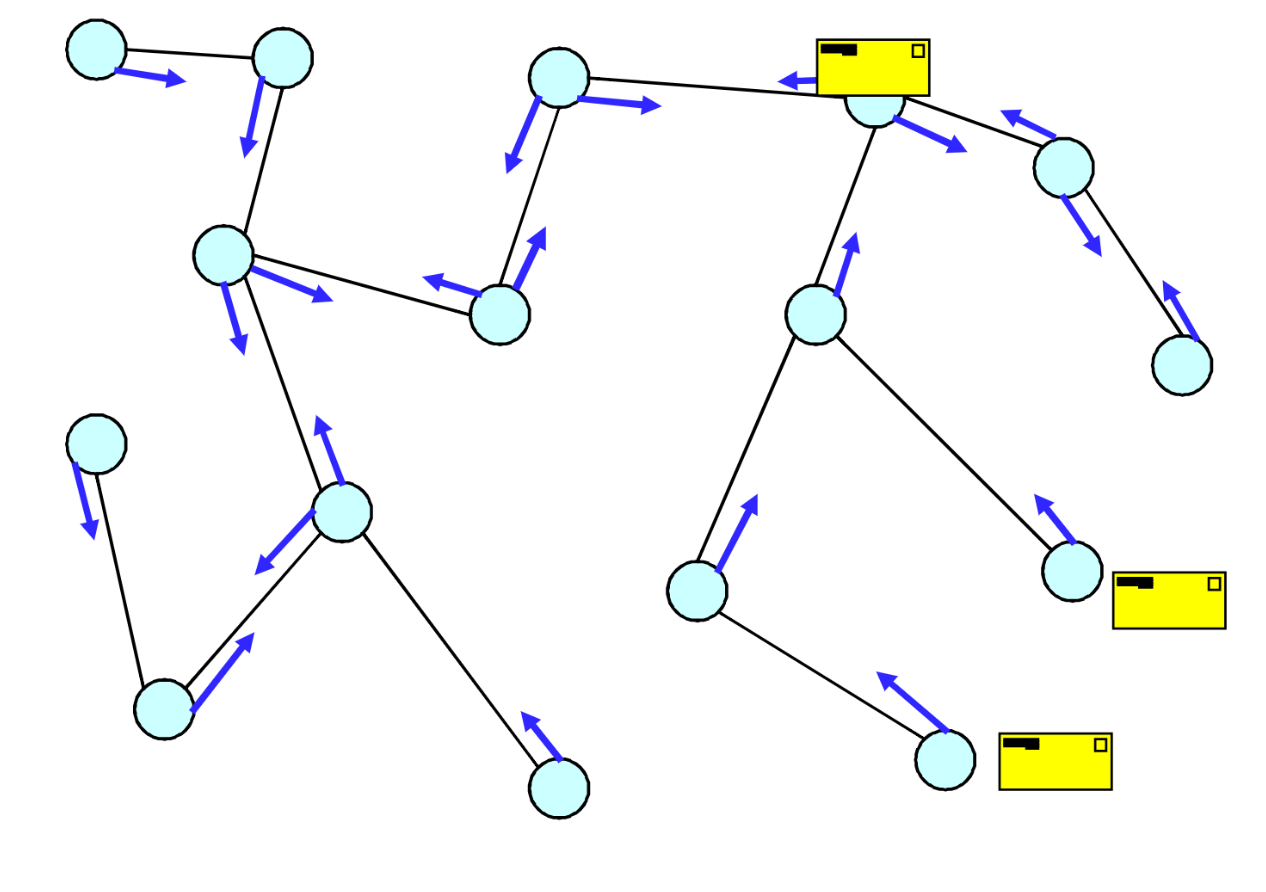
\includegraphics[width=100pt]{images/subscription-forwarding.png}\hspace*{\fill}
  \label{fig:subscription-forw}
\end{figure} \\
\subparagraph{Hierarchical forwarding}
There is a special node that is the root of the network. When someone subscribe to the "blue" subscription, the information goes up to the root and then it will go down to the subscriber following the minimal path. Since the subscription isn't distributed on all the entire network, it cannot be guaranteed that the publication follows the minimal path. 
 \begin{figure}[h!]
 \hfill 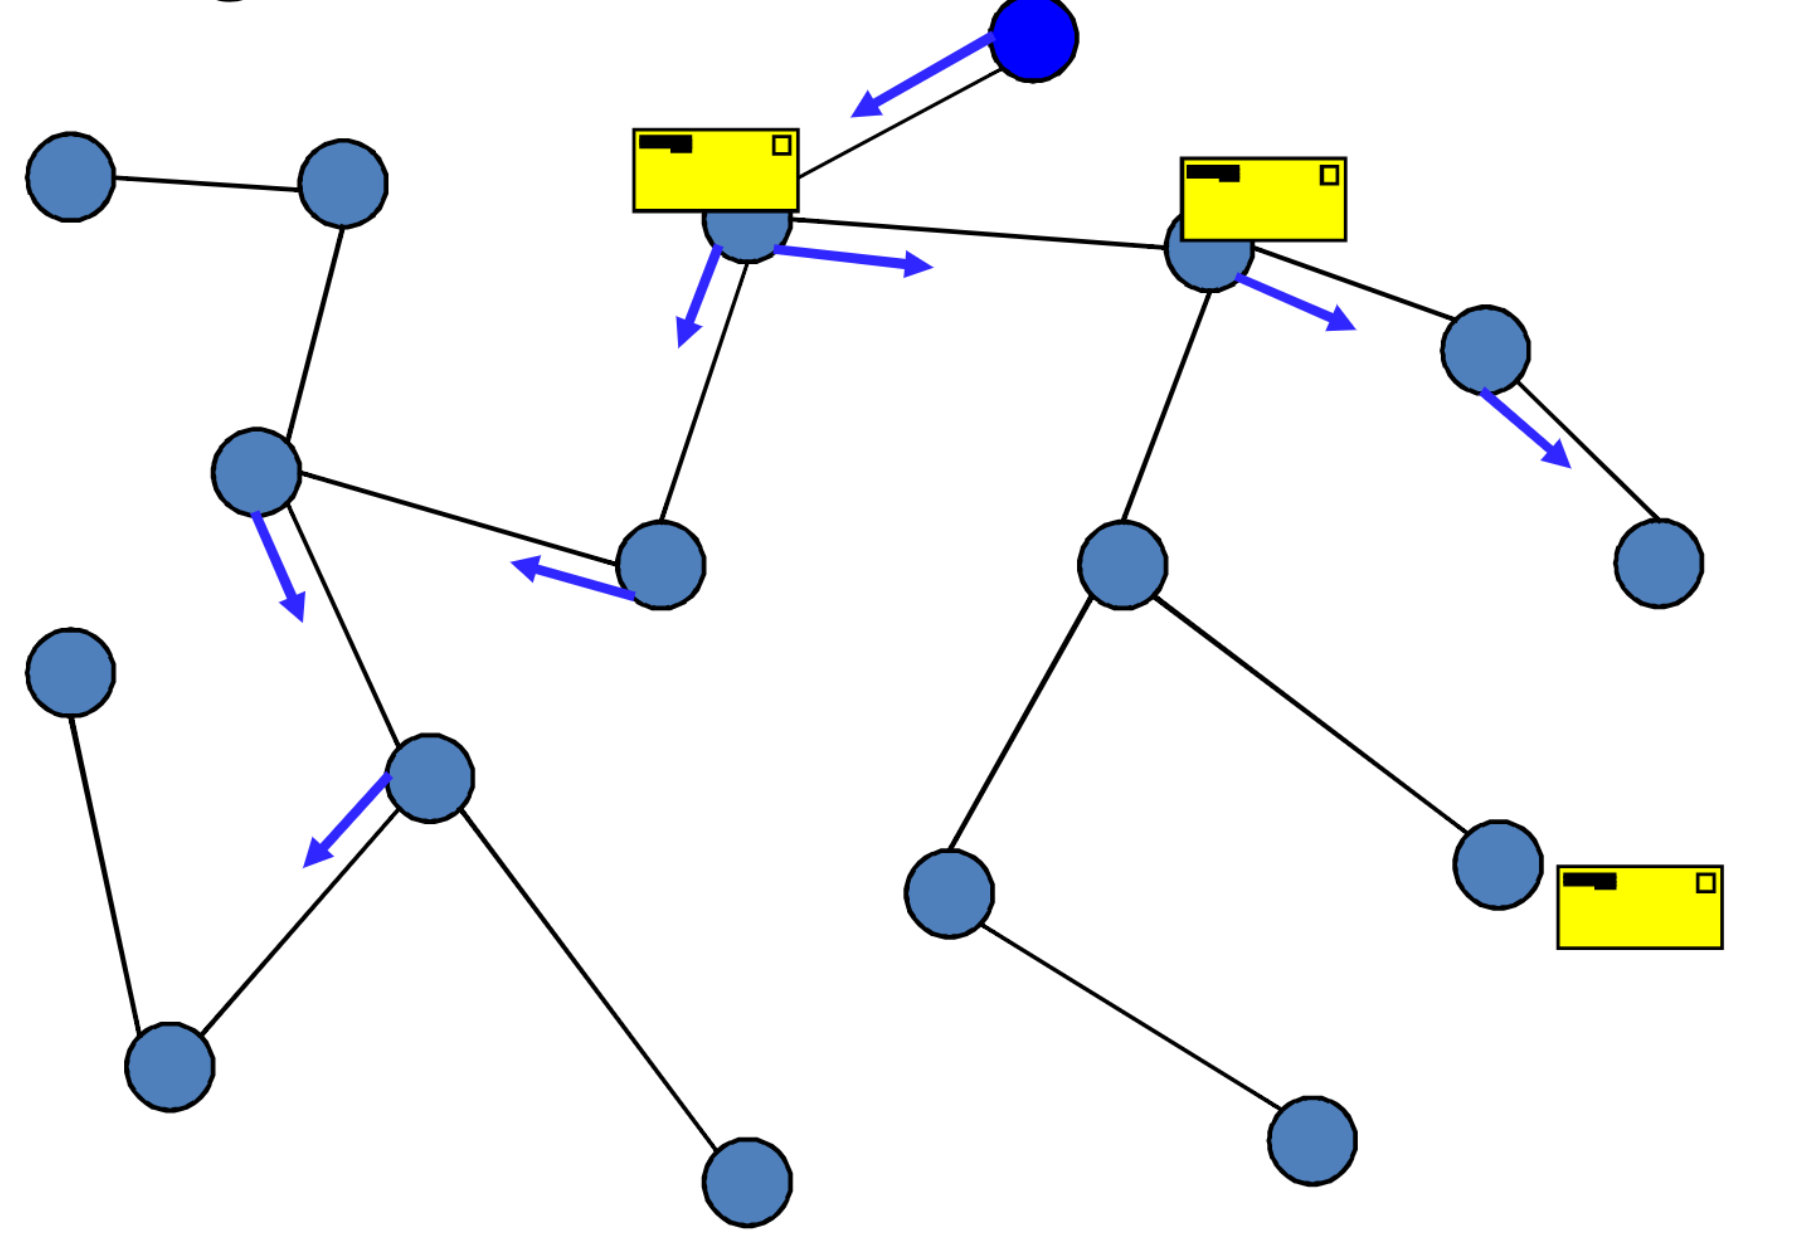
\includegraphics[width=100pt]{images/hierarchical-forwarding.png}\hspace*{\fill}
  \label{fig:hierarchical-forw}
\end{figure}
\paragraph{Cyclic topologies}
\subparagraph{DHT approach}
A \textit{DHT (Distributed Hash Table)} is a distributed hash table, that associates any $\langle key,value \rangle$ pair, and it's distributed on several machines. Given the hash, it identifies a node that contains a specific key and retrieve its value. Each node has its own portion of the DHT.\\
DHT is used to store the huge routing table the publish/subscribe system. For each topic is stored a key on the DHT with value the list of subscribers, to know which node is interested in that topic.
\\ To subscribe for messages having a given subject $S$:
\begin{enumerate}
	\item Calculate a hash of the subject $H_S$
	\item Use the DHT to route toward the node $succ(H_S)$
	\item While flowing toward $succ(H_S)$ leave routing information to return messages back
\end{enumerate}
 To publish a message having a given subject $S$:
\begin{enumerate}
	\item Calculate a hash of the subject $H_S$
	\item Use the DHT to route toward the node $succ(H_S)$
	\item While flowing toward $succ(H_S)$ follow back routes towards subscribers
\end{enumerate}
\subparagraph{Content-based routing}
Useful to differentiate between \textit{forwarding} and \textit{routing}. \\
There are different routing strategies:
\begin{itemize}
	\item Per source forwarding (PSF)
	\item Improved per source forwarding (iPSF)
	\item Per receiver forwarding (PRF)
\end{itemize}
and different strategies to build paths:
\begin{itemize}
	\item Distance Vector (DV)
	\item Link-State (LS)
\end{itemize}
\paragraph{Complex Event Processing}
\textit{CEP} systems adds the ability to deploy rules that describe how composite events can be generated from primitive (or composite) ones. The idea is to move part of the logic into the middleware (broker). The broker is called complex event processing engine. \\ \\
\textit{Example:} \\
The publishers are sensors in a sensor network (temperature, humidity and smoke sensors), the subscribers are the alarm systems. The publisher publishes messages like "temperature = 20" or "smoke detected". The subscribers are not interested in temperature reading, neither in smoke reading but they are interested only in "possible fire" events. \\
The simple case is that the subscriber evaluate "possible fire" event receiving all the data. The complex engine instead becomes responsible for that evaluation and dispatches that special event to the subscriber. Part of the application is moved to the broker, and the traffic in the network is reduced.
 \begin{figure}[h!]
 \hfill 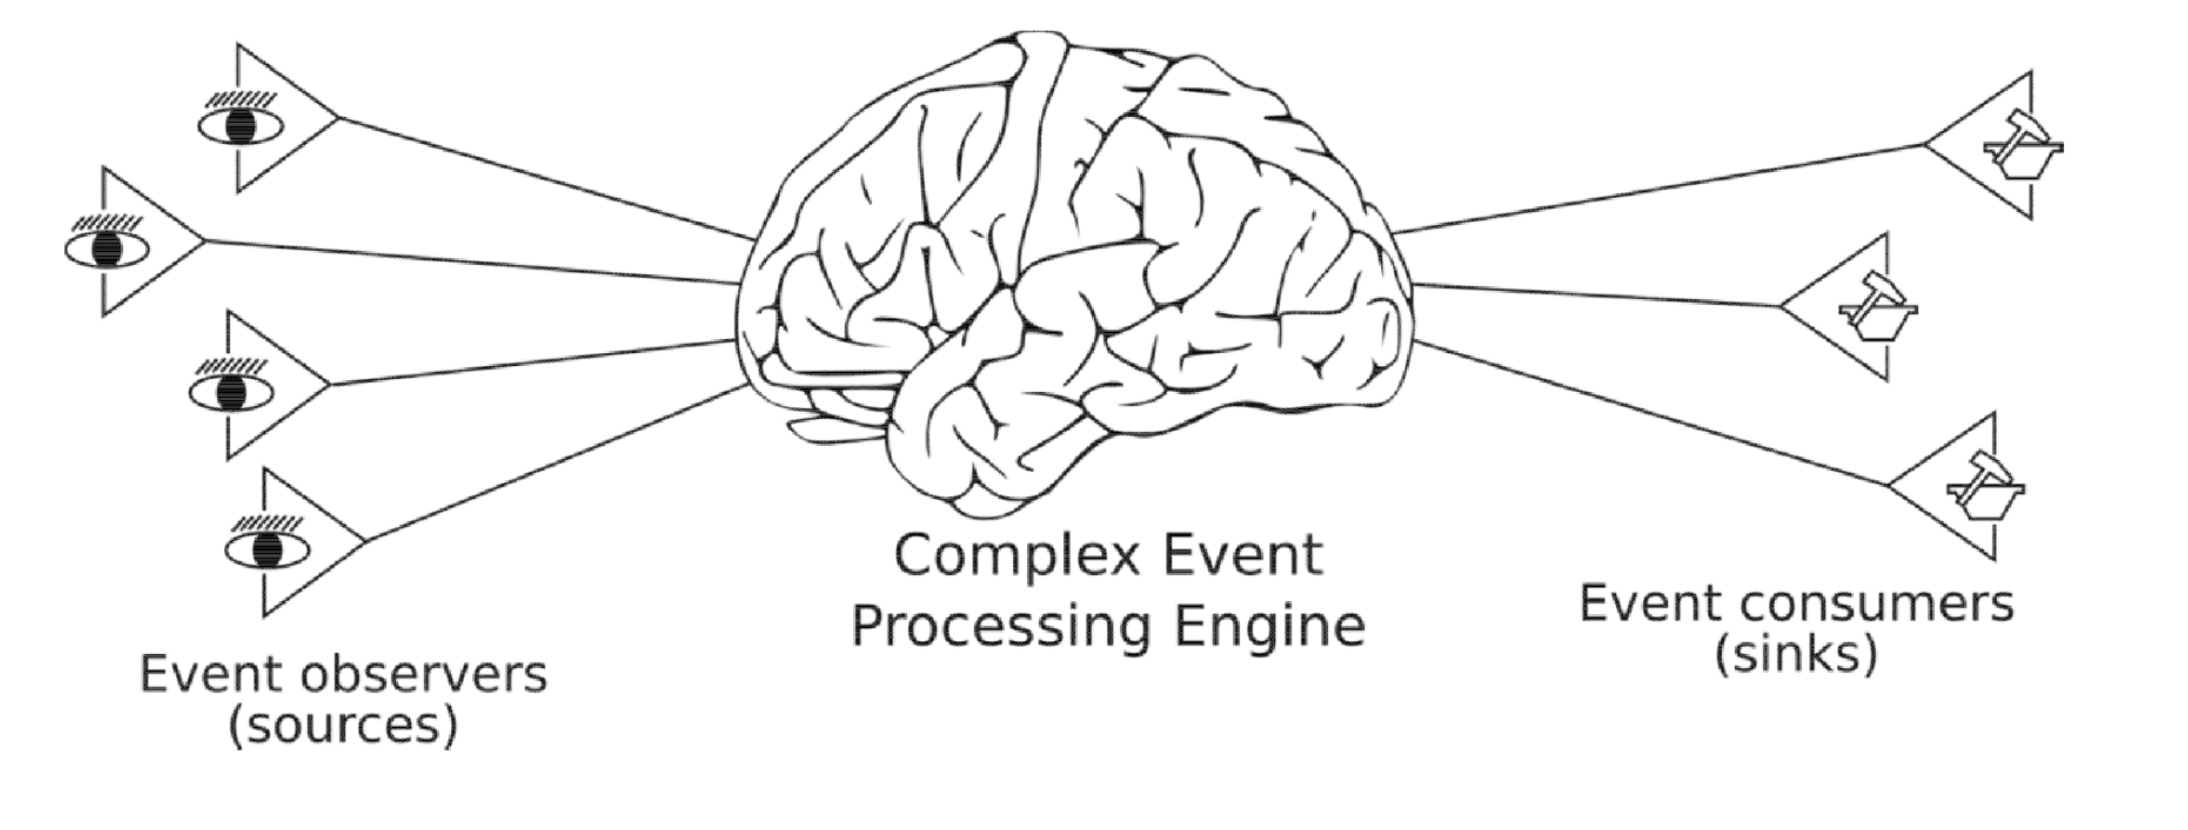
\includegraphics[width=110pt]{images/cep.png}\hspace*{\fill}
  \label{fig:cep}
\end{figure}
\subsection{Stream-oriented communication}
\subsubsection{Fundamentals}
A Data Stream is a sequence of data units. Information is always organized as a sequence of data units. E.g., text, audio... \\
Time usually does not impact the correctness of the communication but just its performance. In some cases this is not the case (e.g., when sending a video "in streaming"). \\
Transmission modes:
\begin{itemize}
	\item \textit{Asynchronous}: the data items in a stream are transmitted one after the other without any further constraints (apart ordering)
	\item \textit{Synchronous}: there is a max end-to-end delay for each unit in the data stream
	\item \textit{Isochronous}: there is a max and min end-to-end delay (bounded jitter)
\end{itemize}
Non-functional requirements are often expressed as \textit{Quality of Service} (QoS) requirements:
\begin{itemize}
	\item Required bit rate
	\item Maximum delay to setup the session
	\item Maximum end-to-end delay
	\item Maximum variance in delay (jitter)
\end{itemize}
 \begin{figure}[h!]
 \hfill 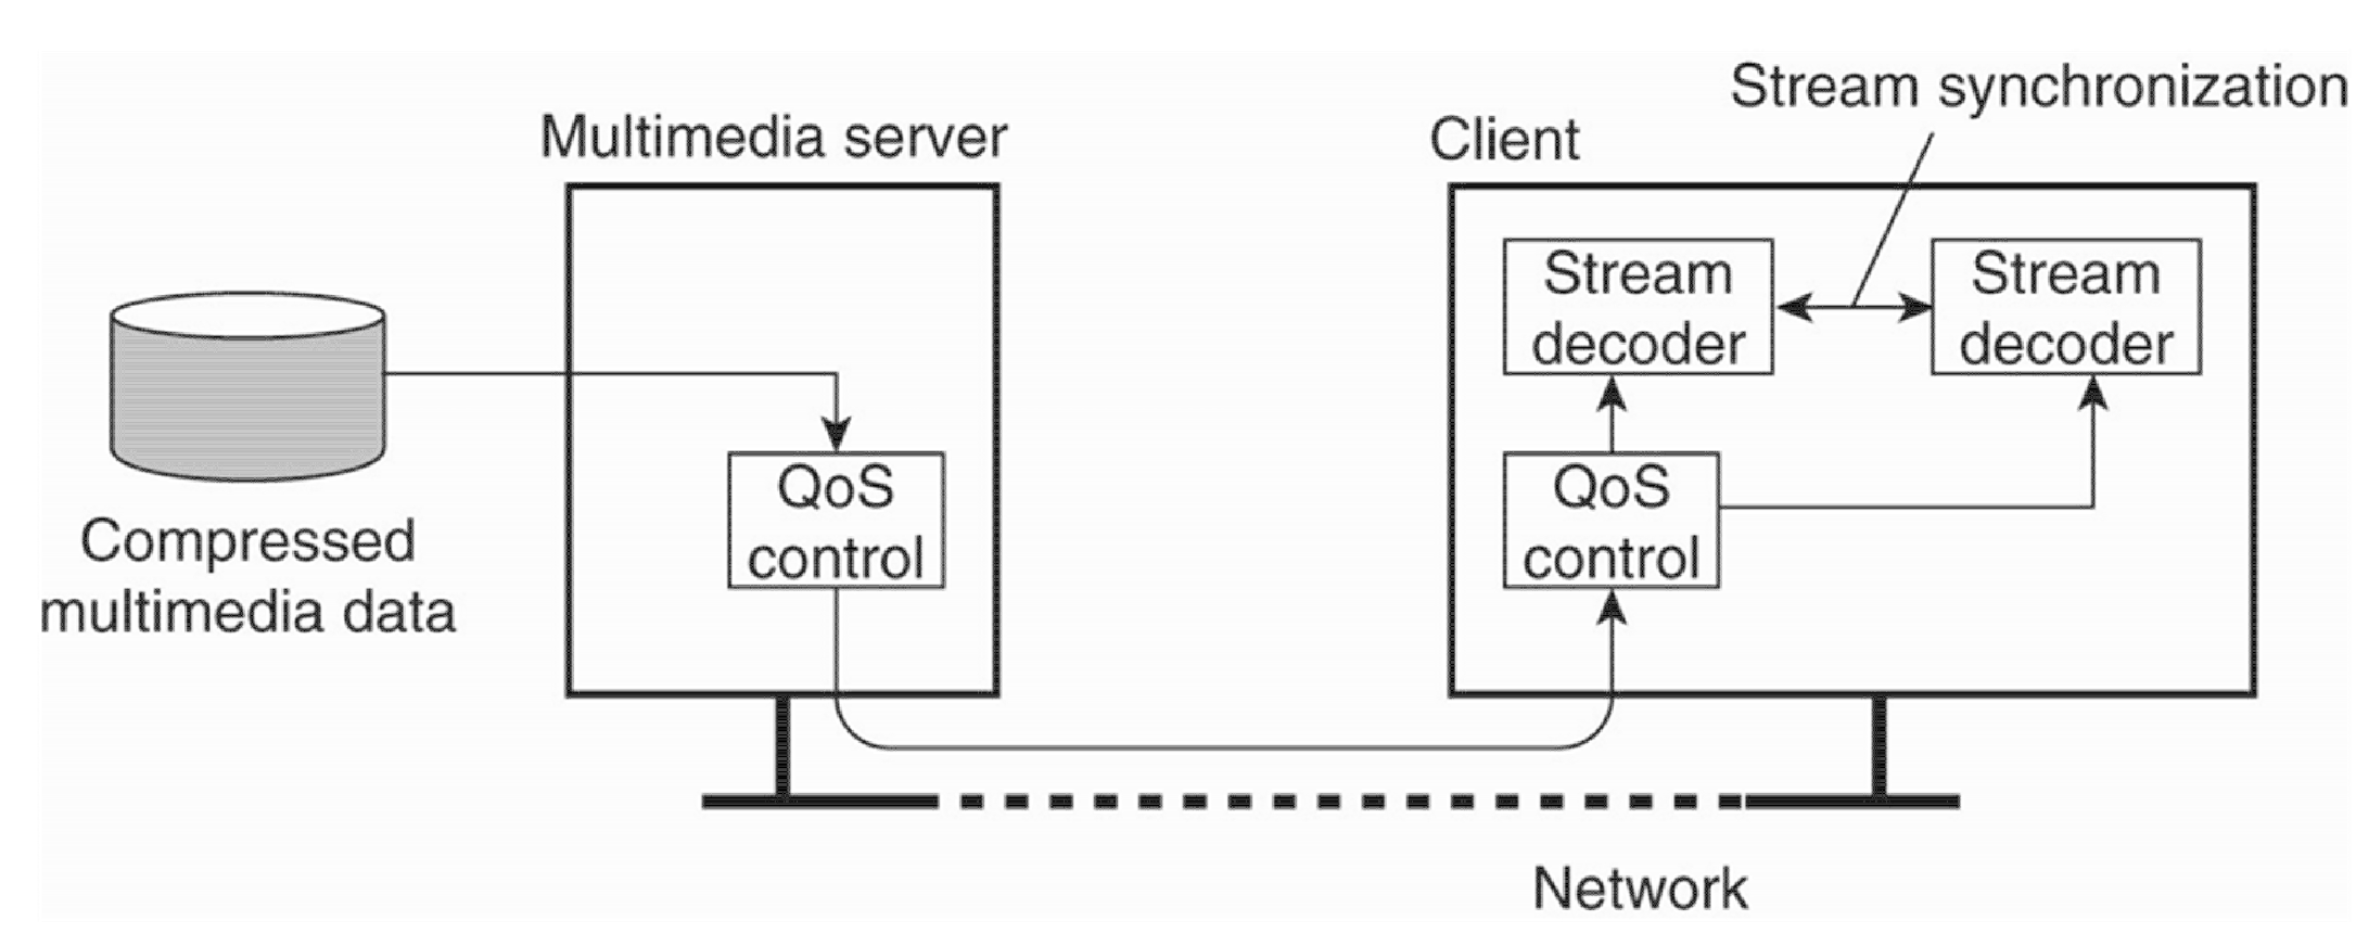
\includegraphics[width=160pt]{images/qos.png}\hspace*{\fill}
  \label{fig:qos}
\end{figure}
\subsubsection{Guaranteeing QoS}
QoS is complex because the internet does not provide any QoS. IP offers a special field of the packet that is the \textit{Type of Service} (ToS) into its header. Based on ToS, routers should privilege some packets w.r.t. to others.\\ \\
One method to enforce QoS at the application layer consists in buffering data. Even tough, if there is too much congestion, the buffer will become empty and the application realizes that there was a problem in the network.
 \begin{figure}[h!]
 \hfill 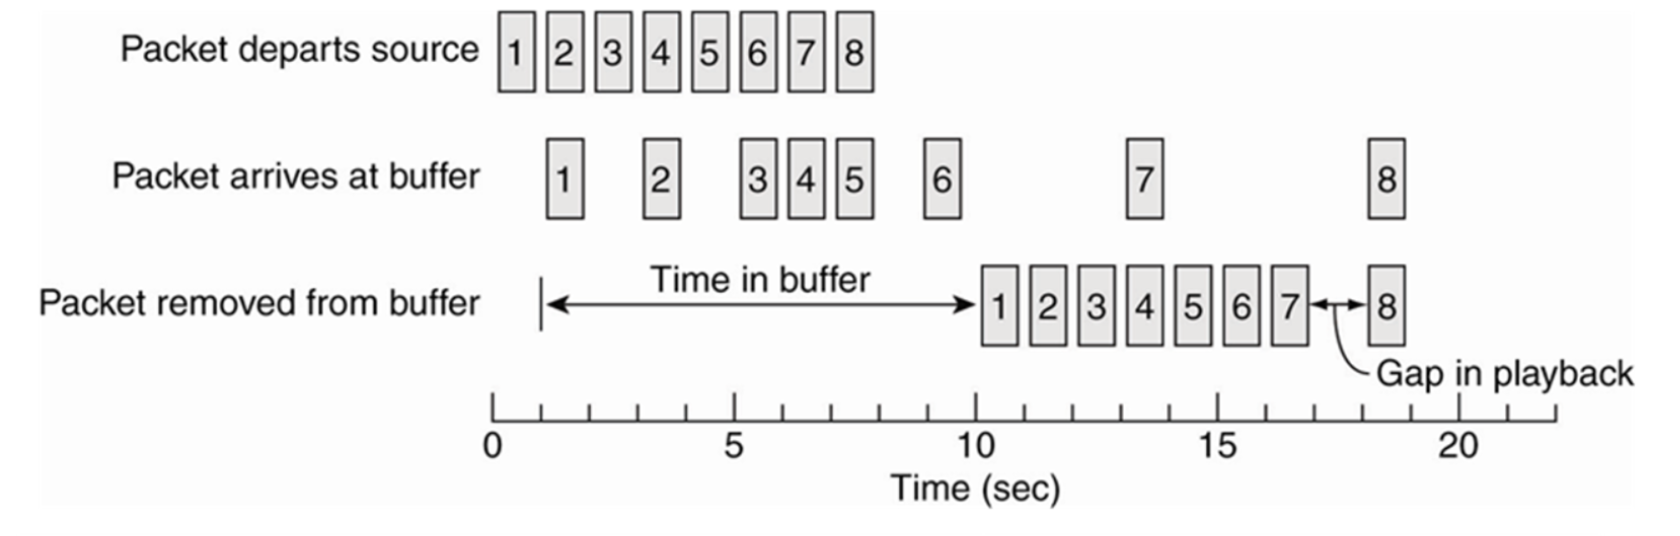
\includegraphics[width=200pt]{images/qos-buffering.png}\hspace*{\fill}
 \caption{QoS buffering}
  \label{fig:qos-buffering}
\end{figure}
  \begin{figure}[h!]
\centering
\begin{minipage}{.5\textwidth}
  \centering
  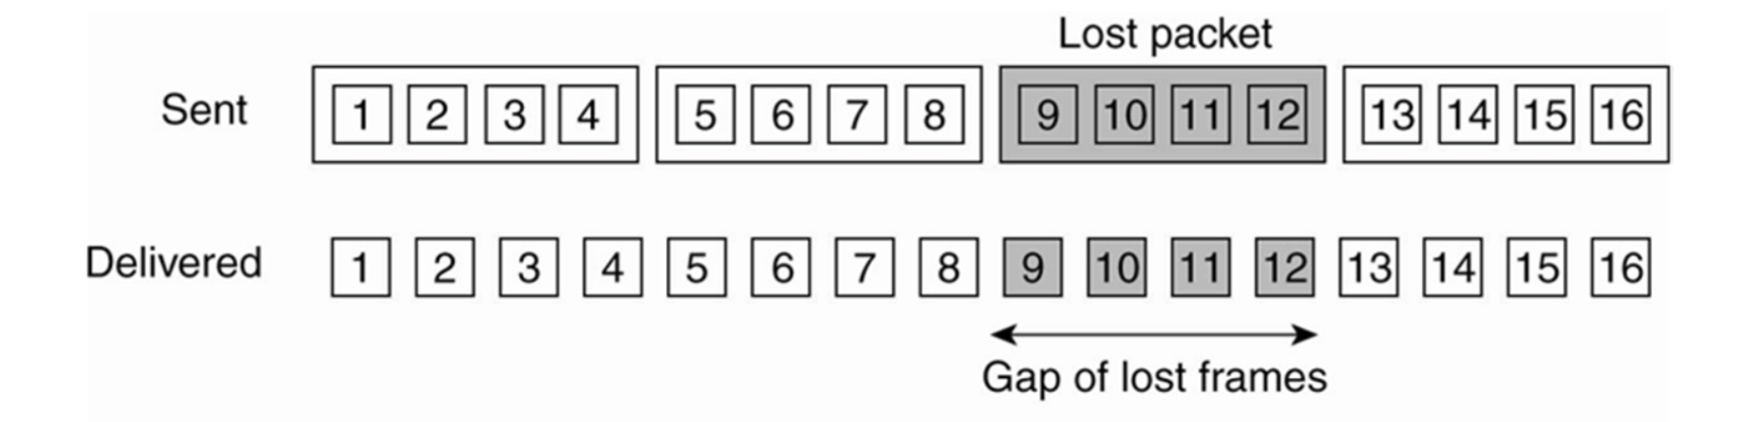
\includegraphics[width=.9\linewidth]{images/qos-forw-err.png}
  \captionof{figure}{QoS forward error correction}
  \label{fig:qos-forw-err}
\end{minipage}%
\begin{minipage}{.5\textwidth}
  \centering
  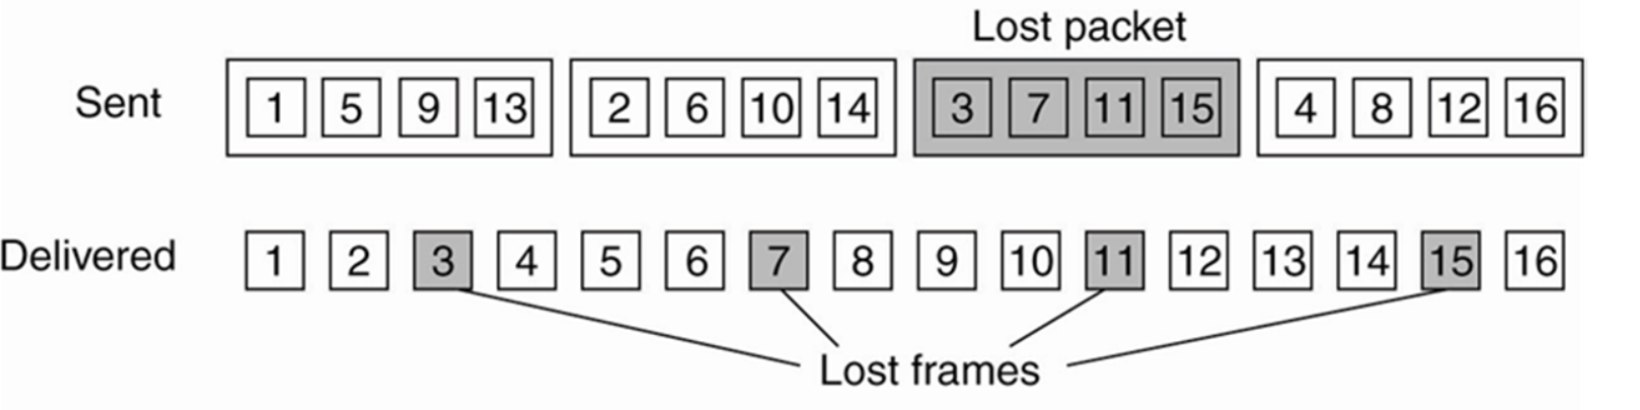
\includegraphics[width=.9\linewidth]{images/qos-interleaving.png}
   \captionof{figure}{QoS interleaving data to mitigate errors}
  \label{fig:qos-interleaving}
\end{minipage}
\end{figure}
Thanks to data interleaving, if we lose a packet, instead of losing a portion of the video, we are losing frames of the video that are spread in the range of 3-4 seconds. The lost frames can be even reconstructed given the other one that are associated to it. \\ \\
Synchronizing two or more streams is not easy, it could mean different things:
\begin{itemize}
	\item Left and right channels at CD quality $\rightarrow$ each sample must be synchronized $\rightarrow$ 23$\mu$sec of max jitter
	\item Video and audio for lip synch $\rightarrow$ each audio interval must be in synch with its frame $\rightarrow$ at 30fps 33msec of max jitter
\end{itemize}
Synchronization may take place at the sender or the receiver side, in the former case the different streams can be merged together. It may happen at different layers (application vs. middleware).
 \begin{figure}[h!]
 \hfill 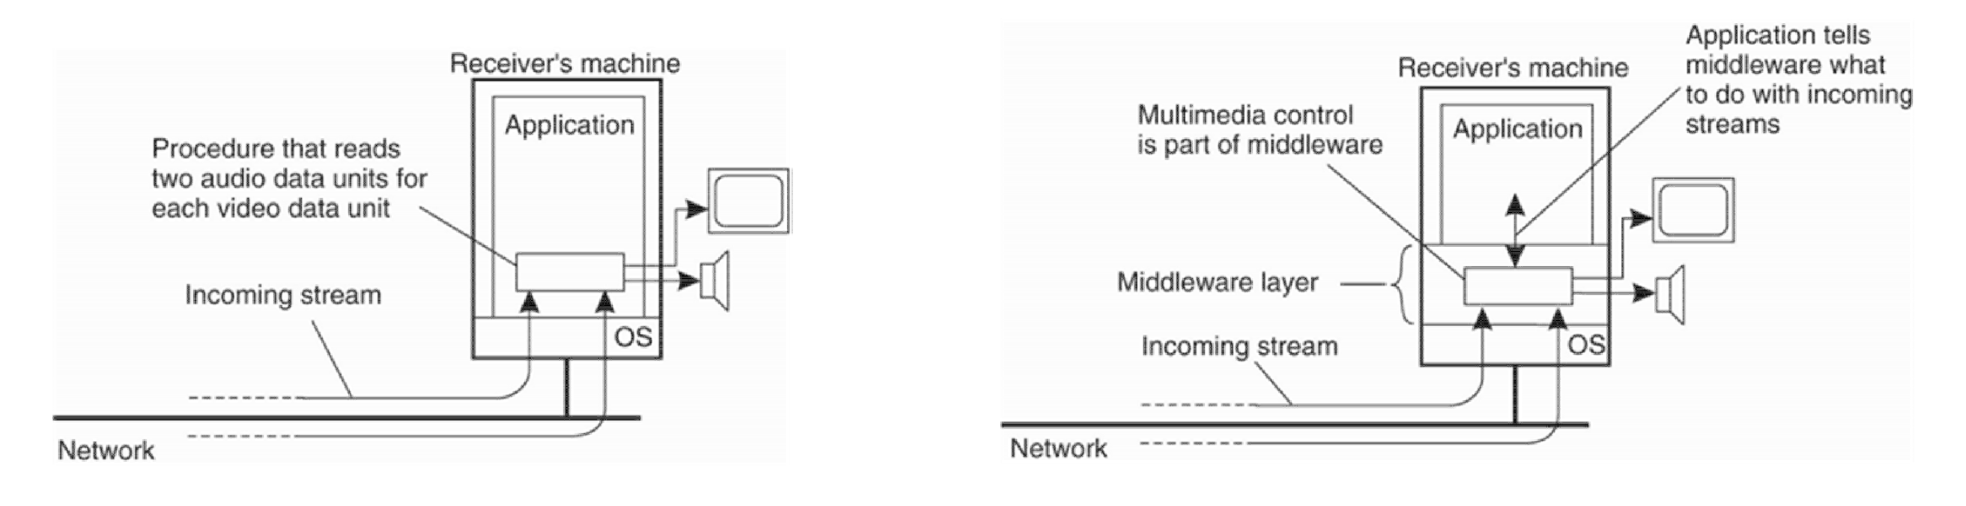
\includegraphics[width=250pt]{images/qos-sync.png}\hspace*{\fill}
 \caption{QoS synchronization}
  \label{fig:qos-sync}
\end{figure}
\section{\LARGE Naming}
\subsection{Basics}
\subsubsection{Entities, names, addresses, identifiers}
\textit{Names} are used to refer to \textit{entities}: hosts, users, files, services, ... \\ Entities are usually accessed through an \textit{access-point} (ethernet, Wi-Fi), a special entity characterized by a special name that is the \textit{address}. \\
The same entity can be accessed through several access points at the same time and it can change its access-points during its lifetime. \textit{e.g., When I am in the office I can be reached through e-mail, cell-phone, office phone. My notebook changes its network (and consequently its IP address) while I move from office to home.} \\
Consequence: it is not convenient to used the address of its access points as a name for the entity, it's better using \textit{location-independent} names (they do not depend on the access point used to access an entity. \\ 
A \textit{global name} denotes the same entity, no matter where the name is used. While the interpretation of a \textit{local name} depends on where it is being used. \\
Instead of having names associated to the various addresses, is better to have names associated with an entity ID, that is associated with the various addresses. Going from name to identifier and from the identifier to the specific address that is valid at that time.\\ \textbf{Identifiers} are names such that:
\begin{itemize}
	\item They never change (during the lifetime of the entity)
	\item Each entity has exactly one identifier
	\item An identifier for an entity is never assigned to another entity
\end{itemize}
Using identifiers enables to split the problem of mapping a name to an entity and the problem of locatin the entity.
 \begin{figure}[h!]
 \hfill 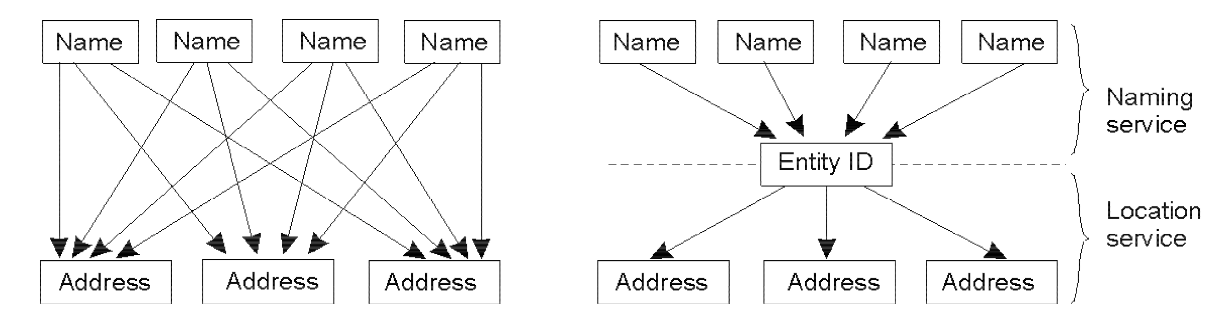
\includegraphics[width=230pt]{images/identifiers.png}\hspace*{\fill}
 \caption{Mapping between name and addresses with and without identifiers}
  \label{fig:identifiers}
\end{figure}
\subsubsection{Name resolution}
\textbf{Name resolution} is the process of obtaining the address of a valid access point of an entity having its name. Examples:
\begin{itemize}
	\item DNS maps domain names to hosts
	\item X500 and LDAP maps a person's name to email, telephone number, ...
	\item The RMI registry maps the name of a Java remote object to its remote reference
	\item UDDI maps the description of a Web service to the service metadata (e.g., a Web server) needed to access it
\end{itemize}
The way name resolution is performed depends on the nature of the naming schema employed:
\begin{itemize}
	\item \textit{Flat naming}
	\item \textit{Structured naming}
	\item \textit{Attribute-based naming}
\end{itemize}
\subsection{Flat naming}
In a \textbf{flat naming} schema names are "flat". They are simple strings with neither structure nor content (e.g., www.google.it is not a flat name because it's a structure; Bluetooth address is an example of flat naming). \\ The name resolution process can be approached in different ways:
\begin{itemize}
	\item Simple solutions (broadcast or multicast-based, forwarding pointers)
	\item Home-based approaches
	\item Distributed hash tables
	\item Hierarchical approaches
\end{itemize}
\subsubsection{Simple solutions}
Simple solutions are designed for small-scale (e.g., LAN) environments.
\begin{itemize}
	\item Broadcast
	\begin{itemize}
		\item Similar to ARP, send "find" message on broadcast channel: only the interested host replies
		\item Drawback: all hosts must process all "find" messages and this adds traffic and computational overhead
	\end{itemize}
	\item Multicast
	\begin{itemize}
		\item Same as broadcast, but send to a multicast address to reduce the scope of the search
		\item Does not scale as well
	\end{itemize}
	\item Forwarding pointers (for mobile nodes)
	\begin{itemize}
		\item Leave reference to the next location at the previous location
		\item Solve the problem of temporary relocation of an entity. Proxies forward requests to the real object instance.
		\item Chains can become very long: broken links cause chain to break and there is increased network latency at dereferencing. Keep chain short by adjusting proxies.
		 \begin{figure}[h!]
 \hfill \includegraphics[width=200pt]{images/forwarding-pointers.png}\hspace*{\fill}
 \caption{Forwarding pointers: adjusting proxies and skeleton dereferencing to keep chain short}
  \label{fig:forw-point}
\end{figure} \\
	\end{itemize}
\end{itemize}
\pagebreak
\subsubsection{Home-based approaches}
\begin{figure}[h!]
 \hfill \includegraphics[width=200pt]{images/home-based.png}\hspace*{\fill}
  \label{fig:home-based}
\end{figure}
\textbf{Home-based approaches} are used in Mobile IP and 2.5G cellphone networks. They rely on one home node that knows the location of the mobile unit. Home is assumed to be stable, and can be replicated for robustness. The original IP of the host is effectively used as an identifier. \\
e.g., A person in Asia wants to contact a number in the USA. The phone number is resolved in the home address. Then the source is informed with the host's present address (location) so that can use the shortest path. \\
Drawbacks:
\begin{itemize}
	\item The extra step towards the home increases latency
	\item The home address has to be supported as long as the entity lives
	\item The home address is fixed, which means an unnecessary burden when the entity permanently moves to another location
	\item Poor geographical scalability (the entity may be next to the client)
\end{itemize}
\subsubsection{Distributed hash tables}
\textbf{Distributed Hash Tables (DHT)} can be used as a directory service (naming service):
\begin{itemize}
	\item key $\rightarrow$ name, where the key is typically a result of an hash function applied over \linebreak (IP Address + port)
	\item value $\rightarrow$ address
\end{itemize} \pagebreak
\textit{Example: CHORD} \\
\begin{figure}[h!]
 \hfill \includegraphics[width=120pt]{images/chord.png}\hspace*{\fill}
  \label{fig:chord}
\end{figure} \\
Chord is a protocol and algorithm for a peer-to-peer distributed hash table.
Nodes and keys are organized in a \textit{logical ring}:
\begin{itemize}
	\item Each node is assigned a unique $m$-bit identifier, usually the hash of the IP address
	\item Every item is assigned a unique $m$-bit key, usually the hash of the item
	\item The item with key $k$ is managed (e.g., stored) by the node with the smallest $id >= k$ (the \textit{successor)}.
\end{itemize}
In the case of the picture above, Node32 will manage K5 and K20. If we have to search K20, we need to find the $n$ node with $n$ that is the smallest number that is greater than 20 (resulting in $n=32$). This method does not scale because complexity is linear w.r.t. the number of keys. There are different method to improve the performance.
\begin{itemize}
\item A possible solution is to implement a \textbf{basic lookup} method where each node keeps track of its successor. In this way, search is performed linearly.
\begin{figure}[h!]
 \hfill \includegraphics[width=120pt]{images/chord-lookup.png}\hspace*{\fill}
  \label{fig:chord-lookup}
\end{figure}
\item In Chord \textbf{finger table} each node maintains a finer table with $m$ entries. Entry $i$ in the finger table of node $n$ is the first node whose id is higher or equal than $n+2^i (i=0...m-1)$. In other words, the $i^{th}$ finger points $1/2^{m-i}$ way around the ring.
\begin{figure}[h!]
 \hfill \includegraphics[width=120pt]{images/chord-finger.png}\hspace*{\fill}
  \label{fig:chord-finger}
\end{figure}
\item In Chord \textbf{routing} a routing table is maintained to keep information about each node. Each row poiints to the next available successors.
 Upon receiving a query for an item with key $k$, a node: 
	\begin{itemize}
		\item Checks whether it stores the item locally
		\item If not, forwards the query to the largest node in the $2^{nd}$
	\end{itemize}
\begin{figure}[h!]
 \hfill \includegraphics[width=160pt]{images/chord-routing.png}\hspace*{\fill}
  \label{fig:chord-routing}
\end{figure}
For instance, taking node 1: successor 2 ($1+2^0)$) is available but successor 3 ($1+2^1$) and 5 ($1+2^2$) are both not available and the first one available is 6. In case node1 is looking for node7, it forwards the query to the largest node in the $succ$ column that does not exceed $k$ (6 in this case). \\ \\
The routing table size (with $N=2^m$ nodes) is $ \log{N}$ fingers. Each hop expects to $1/2$ the distance to the desired id $\Rightarrow$ expects $ O(\log{N})$ hops.
\end{itemize}
\subsubsection{Hierarchical approaches}
The basic idea here is to organize a network as a \textbf{hierarchy}, where each node is responsible for its sub-nodes. \\
The network is divided into domains. The root domain spans the entire network, while leaf domains are typically a LAN or a mobile phone. Each domain has an associated directory node that keeps track of the entities in that domain. 
\begin{figure}[h!]
\centering
\begin{minipage}{.5\textwidth}
  \centering
  \includegraphics[width=.9\linewidth]{images/hierarchical.png}
  \label{fig:hierarchical}
\end{minipage}%
\begin{minipage}{.5\textwidth}
  \centering
  \includegraphics[width=.9\linewidth]{images/hierarchical2.png}
  \label{fig:hierarchical2}
\end{minipage}
\end{figure} 
\begin{itemize}
	\item The root has entries for every entity.
	\item Entries point to the next sub-domain. 
	\item A leaf domain contains the address of an entity (in that domain)
	\item Entities may have multiple addresses (like entity E in figure above) in different leaf domains (replication)
\end{itemize}
Since there's the need to propagate from local nodes (leaves) to the root and going down to the searched leaf, this solution does not scale well, because the more we go up, the bigger is the database that we need, to know where the target node is (the same idea of routing as publish/subscribe acyclic to propagate information). \\ \\
\textbf{Lookup} may start anywhere, where client resides. The client at first looks locally: if not found, forwards lookup to parent. When an entry is found, the responsible node forwards lookup to child until a leaf holding the concrete entry is found.
\begin{figure}[h!]
 \hfill \includegraphics[width=150pt]{images/hierarchical-lookup.png}\hspace*{\fill}
  \label{fig:hierarchical-lookup}
\end{figure}
\textbf{Updates} start with insert request from new location. Location records are created top down or bottom up (bottom up allows for immediate queries). Deleting proceeds from old node up, stopping when a node with multiple children nodes is reached.
\begin{figure}[h!]
 \hfill \includegraphics[width=250pt]{images/hierarchical-updates.png}\hspace*{\fill}
  \label{fig:hierarchical-updates}
\end{figure}
A further optimization consists in \textbf{caching} addresses directly, which is generally inefficient, but with that it is possible to shortcut search if information about mobility patterns is available. \textbf{Scalability}, as said before, is not so high because the root node is expected to hold data for all entities. Records are small, but lookups through root create bottleneck. The root can be distributed, but then allocation of entities to roots becomes tricky (e.g., if user is in the US, assigning it to the portion of the root maintained in Italy is inefficient).
\begin{figure}[h!]
 \hfill \includegraphics[width=250pt]{images/hierarchical-opt.png}\hspace*{\fill}
  \label{fig:hierarchical-opt}
  \caption{After a lookup, server can cache the solution to optimize latency}
\end{figure}
\subsection{Structured naming}
In a \textbf{structured naming} system, names are organized in a \textit{name space}. A name space is a labeled graph composed of \textit{leaf nodes} and a \textit{directory nodes}. \\ A leaf node represents a named entity, it stores information about the entity it refers to. They include, at least, its identifier/address.\\ A directory node has a number of labeled outgoing edges, each pointing to a different node. A node is a special case of an entity. It has an identifier/address. \\
Resources are referred through \textit{path names} (e.g., $\langle alpha,beta,gamma\rangle$ or simply $/alpha/beta/gamma$. Path names can be \textit{absolute} or \textit{relative}. Multiple path names may refer to the same entiti (\textit{hard linking}) or leaf nodes may store absolute path names of the entity they refer to instead of their identifier/address (\textit{symbolic linking}).
\begin{figure}[h!]
\centering
\begin{minipage}{.5\textwidth}
  \centering
  \includegraphics[width=.8\linewidth]{images/structured-hard.png}
  \label{fig:struct-hard}
\end{minipage}%
\begin{minipage}{.5\textwidth}
  \centering
  \includegraphics[width=.8\linewidth]{images/structured-symbolic.png}
  \label{fig:struct-sym}
\end{minipage}
\end{figure} 
\subsubsection{Name spaces and name servers}
\textbf{Name spaces} for a large scale, possibly world wide, distributed system are often distributed among different \textit{name servers}, usually organized hierarchically. \\ 
The name space is partitioned into layers and each node of the name space is assigned to a name server:
\begin{itemize}
	\item \textbf{Global level}: consists of the high-level directory nodes. Main aspect is that these directory nodes have to be jointly managed by different administrations
	\item \textbf{Administrational level}: contains mid-level directory nodes that can be grouped in such a way that each group can be assigned to a separate administration
	\item \textbf{Managerial level}: consists of low-level directory nodes within a single administration. Main issue is effectively mapping directory nodes to local name server
\end{itemize} 
\begin{figure}[h!]
 \hfill \includegraphics[width=150pt]{images/dns.png}\hspace*{\fill}
  \label{fig:dns}
  \caption{The DNS}
\end{figure}
In a DNS, each node holds only the pointers regarding the top portion of a given layer. From the root there are just a few links. Only root knows who is responsible for $com, edu, gov, jp, us,$ etc. We accept that the global layer takes long resolution time because they are stable nodes that can be easily cached. We don't accept that a file take like one hour to propagate an update in the managerial layer.
\begin{figure}[h!]
 \hfill \includegraphics[width=180pt]{images/comparisons-layers.png}\hspace*{\fill}
  \label{fig:comp-layers}
  \caption{Comparisons among layers}
\end{figure}
\paragraph{Name resolution techniques}
\subparagraph{Iterative name resolution}
\begin{figure}[h!]
 \hfill \includegraphics[width=180pt]{images/iterative-dns.png}\hspace*{\fill}
  \label{fig:iterative}
\end{figure}
Iteratively resolve the name asking at first to the root, and then to its sub-nodes, who is the responsible for a certain resource. Then, thanks to caching systems, the next time 'www' is searched instead of 'ftp', the responsible for <nl,vu,cs> is already known, simplifying the resoultion process.
\subparagraph{Recursive name resolution}
\begin{figure}[h!]
 \hfill \includegraphics[width=180pt]{images/recursive-dns.png}\hspace*{\fill}
  \label{fig:recursive}
\end{figure}
This technique is much more inefficient because the number of requests is always the same, without exploiting previous resolutions. Each time the first request asks to root to get the responsible for a certain resource. Then root recursively forwards the request to its sub-nodes and so on. \pagebreak
\begin{figure}[h!]
 \hfill \includegraphics[width=180pt]{images/tradeoff-res.png}\hspace*{\fill}
  \label{fig:tradeoff-res}
\end{figure} \\
There are tradeoffs between the two techniques. \\ Pros of recursive vs. iterative resolution
\begin{itemize}
	\item Communication costs may be reduced
	\item Caching is more effective because it can be performed along the whole resolution chaing, leading to faster lookups
\end{itemize}
Cons:
\begin{itemize}
	\item Higher demand (suspended threads) on each name server
\end{itemize}
\subsubsection{DNS in practice}
In practice, the name space is hierarchically organized as a rooted tree (no hard links).
\begin{itemize}
	\item Each subtree is named \textit{"domain"}, and belongs to a separate authority
	\item Each name server is responsible for a \textit{zone}
\end{itemize}
Name is case-insensitive, up to 255 characters, max 63 characters per "label". Furthermore, each node may represent several entities through a set of \textit{resource records}.
\begin{figure}[h!]
 \hfill \includegraphics[width=180pt]{images/dns-struct.png}\hspace*{\fill}
  \label{fig:dns-struct}
\end{figure} \\
Regarding DNS resolution, clients can request the resolution mode, but servers are not obliged to comply (global name servers typically support only iterative resolution). In practice, a mixture of the two is used. Global servers are mirrored, and IP anycast is used to route queries among them. \\ 
Cachine and replication are massively used: 
\begin{itemize}
	\item Secondary DNS servers are periodically (e.g., twice per day) brought up-to-date by the primary ones.
	\item A TTL attribute is associated to information, determining its persistence in the cache.
\end{itemize}
Transient (days at the global level) inconsistencies are allowed. Only host information is stored, but in principle other information could be stored. \\ \\
DNS works well based on the assumption that:
\begin{itemize}
	\item Content of global/administrational layers is quite stable
	\item Content of managerial layer changes often, but requests are served by name servers in the same zone, therefore updates are efficient
\end{itemize}
What if a host is allowed to "move"? This is not a problem if it stays within the original domains: just update the database of domain name servers. E.g., moving the FTP server \textit{ftp.elet.polimi.it} to a different machine affects only the DNS servers for \textit{elet.polimi.it}. \\
If a host (e.g. \textit{ftp.elet.polimi.it}) moves to an entirely different domain (e.g., \textit{cs.wustl.edu}): 
\begin{itemize}
	\item Better keep its name because applications and users are relying on it
	\item DNS servers of \textit{elet.polimi.it} could provide the IP address of the new location:
	\begin{itemize}
		\item Lookups not affected
		\item Further updates no longer "localized" (managerial layer no longer efficient)
	\end{itemize}
	\item DNS servers of \textit{elet.polimi.it} could provide the name of the new location (essentially a symbolic link). Similar to the forwarding pointers approach:
	\begin{itemize}
		\item Lookups less efficient: essentially two distributed lookups are required
		\item Further updates not affected
	\end{itemize}
\end{itemize}
\subsection{Attributed based naming}
Problem: as more information is made available, it becomes important to effectively search for items. \\
Solution: refer to entities not with their name but with a set of attributes, which code their properties. \\
Each entity has a set of associated attributes. The name system can be queried by searching for entities given the values of (some) of their attributes. Eventually more entities can be returned. Attribute based naming systems are usually called \textit{directory services} and they are usually implemented by using DBMS technology. \\ \\
\textit{Note: the difference between "lookup" and "search":
\begin{itemize}
	\item Lookup means that the name is known and we need to search for the address
	\item Search means that we have some general information about the resource (name is not known), and we want to search name and address of the resource
\end{itemize}
}
\subsubsection{Directory services, LDAP}
A common approach to implement distributed directory services is to combine structured with attribute based naming. \\
The \textbf{LDAP (lightweight directory access protocol)} directory service is becoming the de-facto standard in this field. \\ An LDAP directory consists of a number of records (\textit{directory entries)}:
\begin{itemize}
	\item Each is made as a collection of $\langle$attribute, value$\rangle$ pairs
	\item Each attribute has a type
	\item Both single-valued and multiple-valued attributes exist
\end{itemize}
The collection of all records in a LDAP directory service is called \textit{Directory Information Base - DIB}.\\ Each record has a unique name:
\begin{itemize}
	\item Defined as a sequence of \textit{naming attributes} (aka \textit{relative distinguished name - RDN})
	\item E.g, $/C=NL/ O=Vrije Universiteit/ OU=Comp. Sc./CN=Main server$
\end{itemize}
This approach leads to build a \textit{directory information tree - DIT}. A node in a LDAP naming graph can thus simultaneously represent a directory in a traditional sense (i.e., in a hierarchical name space).
\begin{figure}[h!]
 \hfill \includegraphics[width=200pt]{images/ldap.png}\hspace*{\fill}
  \label{fig:ldap}
\end{figure} \\
When dealing with large scale directories, the DIB is usually partitioned according to the DIT structure (as in DNS)
\begin{itemize}
	\item Each server is known as a \textit{Directory Service Agent - DSA}
	\item The client is known as a \textit{Directory User Agent - DUA}
\end{itemize}
What LDAP adds to a standard hierarchical naming schema is its searching ability (e.g., search ("$(C=NL)(O=Vrije Universiteit)(OU=*)(CN=Main server$)"). In general several DSA have to be accessed to resolve a query. Microsoft's Active Directory is based on LDAP together with several other technologies. \\
Another directory service that is becoming a standard has been developed in the context of grid computing and web services and is known as \textit{Universal DIrectory and Discovery Integration - UDDI}. \\ 
In conclusion, LDAP supports both search and lookup. Thanks to it, it's possible to specify some attributes and search for all the records that holds those attributes. Of course, a database must be used and the DNS is not a real database.
\subsection{Removing unreferenced entities}
Sooner or later it may happen that for some reasons a set of objects is no more reachable from any other node. Those entities needs to be removed. This is done by creating a graph and labelling rechable and non-reachable nodes. \\ Automatic garbage collection is common in conventional systems. Distribution greatly complicates matters, due to lack of global knowledge about who's using what, and to network failures.
\begin{figure}[h!]
 \hfill \includegraphics[width=160pt]{images/removing-ref.png}\hspace*{\fill}
  \label{fig:removing-ref}
\end{figure} \\
\subsubsection{Reference counting, reference listing, distributed mark-and-sweep}
\paragraph{Reference counting}
Every object keeps track of the number of references that have been given around. When an object is created, it has a reference to its creator. When this reference disappear the object reference counter decrease from 1 to 0, so that object knows that has to be removed. \\
Problems:
\begin{itemize}
	\item Reliability (exactly-once message delivery) must be ensured: typically acknowledgments and duplicate detection and elimination
	\item Race condition when passing references among processes
\end{itemize}
\begin{figure}[h!]
 \hfill \includegraphics[width=150pt]{images/ref-counting.png}\hspace*{\fill}
  \label{fig:ref-counting}
  \caption{Passing a reference requires now three messages: potential performance issue in large-scale systems}
\end{figure}
\paragraph{Weighted reference counting}
Each object keeps two numbers, at the beginning equal (128, 128). When a reference is created, a weight is halved and given to the new node. Garbage collect when two numbers becomes the same. This method tries to circumvent the race condition by communicating only counter decrements. \\
Problem: 
\begin{itemize}
	\item only a fixed number of references can be created (starting from 128 and halving, sooner or later we will finish numbers)
\end{itemize}
\begin{figure}[h!]
\centering
\begin{minipage}{.3\textwidth}
  \includegraphics[width=.9\linewidth]{images/ref-a.png}
  \label{fig:ref-a}
\end{minipage}%
\begin{minipage}{.3\textwidth}
  \includegraphics[width=.9\linewidth]{images/ref-b.png}
  \label{fig:ref-b}
\end{minipage}%
\begin{minipage}{.3\textwidth}
  \includegraphics[width=.9\linewidth]{images/ref-c.png}
  \label{fig:ref-c}
\end{minipage}
\end{figure} 
\paragraph{Reference listing}
Instead of keeping track of the number of references, keep track of the identities of the proxies. \\
Advantages:
\begin{itemize}
	\item Insertion/deletion of a proxy is \textit{idempotent}
	\begin{itemize}
		\item Insertion and deletion of references must still be acknowledged, but requests can be issued multiple times with the same effect
		\item Non-reliable communication can be used
	\end{itemize}
	\item Easier to maintain the list consistent w.r.t. network failures
	\begin{itemize}
		\item e.g., by periodically "pinging" clients (potential scalability problem)
	\end{itemize}
\end{itemize}
Still suffers from race conditions when copying references. \\
Used by Java RMI:
\begin{itemize}
	\item A client creates a local proxy only after it received from the server an acknowledgment to its insertion request
	\item Network failures are dealt with using leases: it is up to the client to "refresh" the reference (potential problems for long failures)
	\item The lease interval is determined by run-time and non negotiable
	\item UDP is used as a transport layer for garbage collection
\end{itemize}
\paragraph{Mark-and-sweep}
How to detect entities disconnected from the root set?
Tracing-based garbage collection techniques: require knowledge about all entities, therefore they have inherent poor scalability. \\
\textit{Mark-and-sweep} on uniprocessor systems
\begin{itemize}
	\item First phase marks accessible entities by following references
	\begin{itemize}
		\item Initially all nodes are white
		\item A node is colored grey when reachable from a root (but some of tis references still need to be evaluated)
		\item A node is colored black after is turned grey and all its outgoing references have been marked grey
	\end{itemize}
	\item Second phase exhaustively examines memory to locate entities not marked and removes them
	\begin{itemize}
		\item Garbage collects all white nodes
	\end{itemize}
\end{itemize}
Mark-and-sweep can also be applied in distributed systems. \\
Garbage collector run on each site: manage proxies, skeletons, and actual objects, initially all marked white. \\
Marking process:
\begin{itemize}
	\item An object in process $P$, and reachable from a root in $P$ is marked grey together with all the proxies in it
	\item When a proxy $q$ is marked grey, a message is sent to its associated skeleton (and object)
	\begin{itemize}
		\item An object is marked grey as soon its skeleton is
		\item Recursively, all proxies in the object are marked grey
	\end{itemize}
	\item An acknowledgment is expected before turning $q$ black
\end{itemize}
Sweep process:
\begin{itemize}
	\item All white objects are collected locally
	\item Can start as soon as all local object are either black or white
\end{itemize}
Problems:
\begin{itemize}
	\item Requires reachability graph to to remain stable
	\item Distributed transaction blocking the entire system
	\item In general scalability issue
\end{itemize}
\section{\LARGE Consistency and Replication}
\subsection{Replication: why?}
The main reason behind replication is \textbf{performance improvement}. \\
Replication allows:
\begin{itemize}
	\item Sharing of workload to increase the \textit{throughput} of served requests and reduce the \textit{latency} for individual requests. For example, replicate a Web server to sustain a higher number of users.
	\item Replicate data close to the users to reduce the \textit{latency} for individual requests. For example, cache in processors, local cache in browsers, geo-replicated services, ...
	\item Increase availability
	\begin{itemize}
		\item Data may be available only intermittently in a mobile setting. A local replica in the mobile node can provide support for disconnected operations.
		\item Data might become unavailable due to excessive load. For example, release of a new operating system.
	\end{itemize}
	\item Achieve fault tolerance
	\begin{itemize}
		\item Related to availability
		\item Data may become unavailable due to failure. 
		\begin{itemize}
			\item $Availability = 1-p^n $\\ where $p$ is the probability of failure, $n$ is the number of replicas
		\end{itemize}
	\end{itemize}
	\item It becomes possible to deal with incorrect behaviors through redundancy
\end{itemize}
\textit{Examples of replication}:
\begin{itemize}
	\item Domain Name Service (DNS)
	\item Content delivery networks (CDN): geographically distributed network that replicate the content to better serve end users
	\item Distributed file systems: file replication allows for faster access and disconnected operations
	\begin{itemize}
		\item User files are reconciled against servers upon reconnection
		\item Assumption: conflicts (files modified by more than a user) are infrequent
	\end{itemize}
	\item Platforms for Big Data
	\begin{itemize}
		\item Rely on distributed file systems
		\item Performance through local access: don't move the data, move the computation.
		\item Fault tolerance through replication
	\end{itemize}
\end{itemize}
\subsubsection{Challenges}
\textbf{Main problem}: \textit{consistency} across replicas. \\ Changing a replica demands changes to all the others. What happens if multiple replicas are updated concurrently?
\begin{itemize}
	\item Write-write conflicts / read-write conflicts
	\item What is the behavior in the case of conflicts?
\end{itemize}
\textbf{Goal}: provide consistency with limited communication overhead. \\ \\
Tradeoffs:
\begin{itemize}
 \item \textit{Scalability vs. Performance}: replication may actually degrade performance.
 \item \textit{Data-centric vs. Client-centric}: different consistency requirements depending on the application scenario.
\end{itemize}
\subsection{Consistency}
\textbf{Challenge}: multiple processes reading and writing on their local copies, propagating their actions in the system. We want to provide consistency of data, so that a read shows always the last updated value of a given resource. \\
Focus on a distributed data store:
\begin{itemize}
	\item Shared memory, file system, database, ...
	\item The store consists of multiple items: files, variables, ...
\end{itemize}
Ideally, a read should show the result of the last write. What does \textit{last mean}? In distributed systems there isn't a global clock, so is impossible to determine it.
\subsubsection{Consistency models}
A \textbf{consistency model} is a contract between the processes and the data store. \\
Tradeoffs: guarantees, performance, ease of use
\begin{itemize}
	\item Stricter guarantees simplify the development but incur higher costs
	\item Weaker guarantees reduce the cost but make development difficult
\end{itemize}
There are several different models for individual operations or groups of operations:
\begin{itemize}
	\item Guarantees on content: maximum "difference" on the versions stored at different replicas.
	\begin{description}
		\item \textit{E.g., e-commerce selling t-shirts: if we are saving the number of t-shirts available on different replicas, this number needs to be guaranteed always greater than zero, otherwise people cannot buy their product.}
	\end{description}
	\item Guarantees on staleness: maximum time between a change and its propagation to all replicas.
	\begin{description}
		\item \textit{E.g., If our computer breaks, we want to have a copy (backup) that is at least from yesterday, so that we didn't lost so much data.}
	\end{description}
	\item Guarantees on the order of updates: constraint the possible behaviors in the case of conflicts (data-centric vs. client-centric)
\end{itemize}
\subsubsection{Consistency protocols}
\textbf{Consistency protocols} implement consistency models. \\
There are different strategies for different assumptions/configurations:
\begin{itemize}
	\item Passive vs. Active
	\item Single leader vs. Multiple Leader vs. Leaderless
	\item Synchronous vs. Asynchronous
	\item "Sticky" clients vs. Mobile clients
\end{itemize}
\myparagraph{Passive vs. Active replication}
In \textbf{passive replication} all the operations go through a master. The master propagates all the changes to one or more backup replicas. If the master fails, one of the replicas take over being elected as master. \\
Fault-tolerance is provided only if the propagation of changes occurs synchronously. \\
In this strategy there is no sharing of workload. For this reason, many solutions adopts \textbf{active replication} where replicas can also process user requests.
\myparagraph{Single leader vs. Multiple leaders vs. Leaderless}
In \textbf{single leader} one of the replicas is designated as the leader. When clients want to write to the database, they must send the request to the leader, which first writes the new data to its local storage. \\ The other replicas are known as \textit{followers}. Whenever the leader writes new data to its local storage, it also sends the data to all of its followers. \\
When a client wants to read from the database, it can query any replica (either the leader or a follower). \\ \\
In \textbf{Multiple leaders} writes are carried out at different replicas concurrently. No leader means that there is no single entity that decides the order of writes.\\ It is possible to have write-write conflicts in which two clients update the same value almost concurrently. How to solve conflicts depends on the specific consistency model. \\ \\
In \textbf{Leaderless} replication the client directly contacts several replicas to perfrom the writes/reads. \\ Leaderless protocols are also known as \textit{quorum-based} protocols which are similar to voting system. A majority of replicas is needed to agree on the write. It is also needed an agreement on the value to read.
\myparagraph{Synchronous vs. Asynchronous}
In \textbf{synchronous} protocols the write operation completes after the leader has received a reply from all the followers. \\ \\
In \textbf{asynchronous} protocols the write operation completes when the new value is stored on the leader. Followers are updated asynchronously. \\ \\
\textbf{Semi-synchronous} is a mix between these two in which the write operation completes when the leader has received a reply from at least $k$ replicas.
\subsection{Data-centric consistency models}
From now on we will review the most widely used data-centric consistency models. \\
Graphical convention:
\begin{itemize}
	\item One line for each process
	\item Operations of each process appear in temporal order
	\item Operations of different processes in the same column does not mean that they happen in the same time instant
	\item W(x)a means that the value $a$ is written on the data item $x$
	\item R(x)a means that the value $a$ is read from the data item $x$
\end{itemize}
\subsubsection{Strict consistency}
\mydefinition{Any read on data item x returns the value of the most recent write on x} All writes are instantaneously visible, global order is maintained. "Most recent" is ambiguous without a global time. In practice is possible only within a uniprocessor machine.
\begin{figure}[h!]
 \hfill \includegraphics[width=200pt]{images/strict.png}\hspace*{\fill}
  \label{fig:strict}
  \caption{The example on the right is NOT consistent because P2 reads at first NIL and then A without any write in between}
\end{figure}
\subsubsection{Sequential consistency}
\mydefinition{The result is the same as if the operations by all processes were executed in some sequential order, and the operations by each process appear in this sequence in the order specified by its program}
In \textbf{sequential consistency} operations within a process may not be re-ordered. It is needed that all processes see the same interleaving of operations without considering time.
\begin{figure}[h!]
 \hfill \includegraphics[width=200pt]{images/sequential.png}\hspace*{\fill}
  \label{fig:sequential}
  \caption{The example on the right is NOT consistent because P3 reads $b$ and then $a$, while P4 reads at first $a$ and then $b$.}
\end{figure} \\
In Java values can be read from the local cache and any old value is allowed unless:
\begin{itemize}
	\item The variable is declared as volatile (used to force the process not getting the cached value), or
	\item There is a synchronized block, which are sequentially consistent
\end{itemize}
In practice, synchronization is almost always controlled through synchronized blocks. Cases like the example above should never occur. \\
Consider the following program:
\begin{figure}[h!]
\centering
\begin{minipage}{.5\textwidth}
  \centering
  \includegraphics[width=.9\linewidth]{images/sequentially1.png}
  \label{fig:sequentially1}
\end{minipage}%
\begin{minipage}{.5\textwidth}
  \centering
  \includegraphics[width=.9\linewidth]{images/sequentially2.png}
  \captionof{figure}{All these executions (and many others) are sequentially consistent}
  \label{fig:sequentially2}
\end{minipage}
\end{figure} 
\myparagraph{Implementation}
All the replicas need to agree on a given order of operations. Solutions:
\begin{itemize}
	\item Distributed agreement 
	\item Use a single coordinator: single leader replication (used by MySQL, MongoDB, PostgreSQL, ...)
\end{itemize}
Important assumption: \textit{"Sticky"} clients (not mobile). \\ \\
Sequential consistency limits availability:
\begin{itemize}
	\item We need to contact the leader, which might be further away from the client
	\item The leader must propagate the update to the replicas, in a synchronous way if we want to be fault-tolerant
\end{itemize}
Two main problems related to availability
\begin{itemize}
	\item High latency
	\item Clients are blocked in the case of network partitions
	\begin{itemize}
		\item Can only proceed if they can contact the leader
		\item The leader can only proceed if it can contact the followers
	\end{itemize}
\end{itemize}
That's why a solution consist in the use of leaderless protocols which are \textit{quorum-based}:
\begin{itemize}
	\item An update occurs only if a quorum of the servers agrees on the version number to be assigned
	\item Reading requires a quorum to ensure latest version is being read
	\item Typically:
	\begin{itemize}
		\item $NR + NW > N$ to avoid read-write conflicts
		\item$NW > N/2$ to avoid write-write conflicts
		\item \textit{where $NR(NW)=$ number of replicas that the clients connects to read (write) and $N=NR+NW$}
	\end{itemize}
\end{itemize}
\begin{figure}[h!]
 \hfill \includegraphics[width=200pt]{images/leaderless.png}\hspace*{\fill}
  \label{fig:leaderless}
\end{figure}
\subsubsection{Linearizability}
\mydefinition{The system is sequentially consistent; moreover, if $ts_{OP1}(x)<ts_{OP2}(y)$ then operation $OP1(x)$ precedes $OP2(y)$ in the operation sequence}
\textbf{Linearizability} is stronger than sequential, but weaker than strict. It assumes globally available clocks but only with finite precision. It is useful if the application logic needs to enforce some ordering between operations. \\
The previous example of sequential is also linearizable if we assume the write at P1 has a timestamp greater than the write at P2.
\subsubsection{Causal consistency}
Consider a group chat discussion:
\begin{itemize}
	\item A says "Distributed systems are the best!"
	\item B says "No way! They are too complex ..."
\end{itemize}
If C first sees B and then A, it cannot understand what is going on. Therefore, everybody else must see A's message before B's one. \\
Consider other two messages
\begin{itemize}
	\item A says "Apple released a new MacBook"
	\item B says "I'm having a lot of fun learning about consistency and replication!"
\end{itemize}
The two messages are not related to each other. The order in which they are seen from other members does not matter. \\ \\
\mydefinition{Writes that are potentially causally related must be seen by all processes in the same order. Concurrent writes may be seen in any order at different machines}
Weakens sequential consistency based on Lamport's notion of happened-before. Lamport's model deals with message passing. Here causality is between reads and writes.
\begin{figure}[h!]
 \hfill \includegraphics[width=200pt]{images/causal.png}\hspace*{\fill}
  \label{fig:causal}
\end{figure} \pagebreak \\
\textbf{Causal consistency} defines a causal order among operations. More precisely, causal order is defined as follows:
\begin{itemize}
	\item A write operations $W$ by a process $P$ is causally ordered after every previous operation $O$ by the same process, even if $W$ and $O$ are performed on different variables.
	\item A read operation by a process $P$ on a variable $x$ is causally ordered after a previous write by $P$ on the same variable.
	\item Causal order is transitive
\end{itemize}
It is not a total order. Operations that are not causally ordered are said to be concurrent. \\
Why causal consitency? 
\begin{itemize}
	\item Easier to guarantee within a distributed environment (smaller overhead)
	\item Easier to implement
\end{itemize}
\myparagraph{Implementation}
Multi-leader implementations are possible (which enable concurrent updates). \\ Writes are timestamped with Lamport's \textit{vector clocks}. Vector clocks are a metadata, that we attach to our write, that inform the systm about what the process knows about other processes. In this way a process knows the causality relations between operations. \\ An update U is applied to a replica only when all the write operations that are possible causes of U have been received and applied, otherwise a read always returns the previous value. \\ \\
The above implementation enables a high degree of availability.
\begin{itemize}
	\item Clients can continue to interact with the store even if they are disconnected from other replicas
	\item The local replica will return an old value but it avoids violation of causality
	\item New writes can also be performed
	\begin{itemize}
		\item The rest of the world will not be informed
		\item The writes that occur in the rest of the world will be concurrent
		\item This is clearly not possible under sequential consistency!
	\end{itemize}
\end{itemize}
\textit{Note: this implementation works only if clients are sticky!}
\subsubsection{FIFO consistency}
\mydefinition{Writes done by a single process are seen by all others in the order in which they were issued; writes from different processes may be seen in any order at different machines}
In other words, in \textbf{FIFO consistency}, causality across processes is dropped. FIFO consistency is also called PRAM consistency (Pipelined RAM): if writes are put onto a pipeline for completion, a process can fill the pipeline with writes, not waiting for early ones to complete.
\begin{figure}[h!]
 \hfill \includegraphics[width=200pt]{images/fifo.png}\hspace*{\fill}
  \label{fig:fifo}
  \caption{The example below  is NOT consistent because in P4 reads operations on $x$ show $c$ and then $b$, while they were written in the opposite order order (FIFO ensures that writes are seen in the order they were issued by the process).}
\end{figure} \\
\myparagraph{Implementation}
This type of consistency is very easy to implement even with multi-leader solutions (concurrent updates). \\
The updates from a process $P$ carry a sequence number. A replica performs an update $U$ from $P$ with sequence number $S$ only after receiving all the updates from $P$ with sequence number lower than $S$. \\
\myparagraph{Consistency models and synchronization}
FIFO consistency still requires all writes to be visible to all processes, even those that do not care. Moreover, not all writes need to be seen by all processes. E.g., those within a transaction/critical section. \\ Some consistency models introduce the notion of synchronization variables. Writes becomes visible only when processes explicitly request so through the variable. Appropriate constructs are provided (e.g., synchronize(S)). \\ It is up to the programmer to force consistency when it is really needed, typically:
\begin{itemize}
	\item At the end of a critical section, to distribute writes
	\item At the beginning of a "reading session" when writes need to become visible
\end{itemize}
\subsubsection{Weak consistency}
\textcolor{MidnightBlue}{
\begin{enumerate}
	\item Access to synchronization variables is sequentially consistent;
	\item No operation on a synchronization variable is allowed until all previous writes have completed everywhere;
	\item No read or write to data are allowed until all previous operations to synchronization variables have completed.
\end{enumerate}}
\textbf{Weak consistency} enforces consistency on a group of operations. It limits only the time when consistency holds, rather than the form of consistency. Data may be inconsistent in the meanwhile.
\begin{figure}[h!]
 \hfill \includegraphics[width=200pt]{images/weak.png}\hspace*{\fill}
  \label{fig:weak}
\end{figure}
\subsubsection{Release consistency}
\textbf{Problem}: the data store cannot distinguish between a synchronization request for disseminating writes or for reading consistent data (unnecessary overhead). \\
\textbf{Solution}: introduce different synchronization operations. 
\begin{itemize}
	\item \textit{Acquire} indicates critical region is about to be entered
	\item \textit{Release} indicates critical region has just been exited
	\item In the standard release consistency definition, acquire and release refer to the entire data store.
\end{itemize}
\textcolor{MidnightBlue}{
\begin{enumerate}
	\item Before a read or write is performed, all previous acquires done by the process must have completed successfully;
	\item Before a release is allowed, all previous reads and writes done by the process must have been completed;
	\item Accesses to synchronization variables are FIFO consistent.
\end{enumerate}}
\begin{figure}[h!]
 \hfill \includegraphics[width=200pt]{images/release.png}\hspace*{\fill}
  \label{fig:release}
  \caption{P2's acquire must wait for P1's release}
\end{figure}
On release, protected data that changed are propagated to other copies. Two ways to achieve this:
\begin{itemize}
	\item Eager release consistency
	\begin{itemize}
		\item On release, all updates are pushed to other replicas
		\item Potentially sends data to processes that will not use it
	\end{itemize}
	\item Lazy release consistency
	\begin{itemize}
		\item On release, nothing is sent
		\item On acquire, acquiring process must get latest version of the data from other processes
		\item Tends to be more bandwidth efficient
	\end{itemize}
\end{itemize}
\subsubsection{Entry consistency}
\textbf{Entry consistency} explicitly associates each shared data item with a synchronization variable. 
\begin{itemize}
	\item Still accessed through acquire and release
	\item Reduces update overhead, increase complexity access
	\item Improves parallelism, enabling simultaneous access to multiple critical sections
\end{itemize}
Two modes of access to a synchronized variable
\begin{itemize}
	\item \textbf{Non-exclusive}: multiple processes can hold read locks simultaneously
	\item \textbf{Exclusive}: only one process holds the lock to the variable; to be granted, must guarantee that no other process holds (even a non-exclusive) lock.
\end{itemize}
\textcolor{MidnightBlue}{
\begin{enumerate}
	\item An acquire access of a synchronization variable is not allowed to perform w.r.t. a process until all updates to the guarded shared data have been performed w.r.t. that process;
	\item Before an exclusive mode access to a synchronization variable by a process is allowed to perform w.r.t. that process, no other process may hold the synchronization variable, not even in non-exclusive mode;
	\item After an exclusive mode access to a synchronization variable has been performed, any other process' next non-exclusive mode access to that synchronization variable may not be performed until it has performed w.r.t. that variable's owner.
\end{enumerate}}
\begin{figure}[h!]
 \hfill \includegraphics[width=190pt]{images/entry.png}\hspace*{\fill}
  \label{fig:entry}
  \caption{On acquire, all guarded data must be made visible}
\end{figure}
For exclusive mode to be granted, no other process can be holding any kind of lock. After a data item has been accessed in exclusive mode, all future accesses by processes (other than the one that did the write) must go through the acquire process. \\
Complex to use, but may be useful if encapsulated in a distributed object model. 
\begin{figure}[h!]
 \hfill \includegraphics[width=210pt]{images/summary-consistency.png}\hspace*{\fill}
  \label{fig:summary-consistency}
  \caption{Summary of consistency models}
\end{figure}
\subsubsection{Eventual consistency}
The models considered so far are data-centric. This means that they provide a system-wide consistent data view in the face of simultaneous, concurrent updates. However, there are situations where there are:
\begin{itemize}
	\item No simultaneous updates (or can be easily resolved)
	\item Mostly reads
\end{itemize}
\textit{Examples:} Web caches, DNS, Facebook (geo-distributed data stores). \\ \\
In these systems, \textbf{eventual consistency} is often sufficient: updates are guaranteed to eventually propagate to all replicas. \\
This approach is very popular today for three reasons:
\begin{itemize}
	\item Very easy to implement
	\item Very few conflicts in practice
	\begin{itemize}
		\item E.g., in Facebook a user often accesses and updates the same replica
		\item Today's networks offer fast propagation of updates.
	\end{itemize}	  
	\item Dedicated data-types (conflict-free replicated data-types)
\end{itemize}
\textbf{Conflit-free replicated data types (CRDTs} guarantee convergence even if updates are received in different orders (commutative semantics). \\ \\
\textit{Example: integer counter} \\
Replicas do not store only the last value but the set of add/remove operations performed. These operations can be applied in any order in different replicas, and yield the same result. \\ \\
\textit{Another example: set} \\
Suppose to have a set, and execute 3 operations on it: $add(a)$, $add(a)$, $remove(a)$. \\
In a traditional implementation these operations are not commutative:
\begin{itemize}
	\item $add(a)$, $add(a)$, $remove(a)$ leaves the set empty
	\item $add(a)$, $remove(a)$, $add(a)$ leaves $a$ in the set
\end{itemize}
A commutative set stores all the updates: if there are two $add$ and one $remove$, the element is still there. This is a different semantics w.r.t. traditional sets but guarantees convergence under eventual consistency. \\
There is a reasonable trade-off between performance and complexity. Eventual consitency is often used in geo-replicated data stores. \pagebreak
\subsection{Client-centric consistency models}
What happes if a client dynamically changes the replica it connects to? This problem is addressed by \textbf{client-centric consistency} models that provide guarantees about accesses to the data store from the perspective of a single client.
\begin{figure}[h!]
 \hfill \includegraphics[width=200pt]{images/client-centric.png}\hspace*{\fill}
  \label{fig:client-centric}
\end{figure}
\subsubsection{Monotonic reads}
\mydefinition{If a process reads the value of a data item $x$, any successive read operation on $x$ by that process will always return that same value or a more recent value}
Once a process reads a value from a replica, it will never see an older value from a read at a different replica.
\begin{figure}[h!]
 \hfill \includegraphics[width=200pt]{images/monotonic-reads.png}\hspace*{\fill}
  \label{fig:monotonic-reads}
  \caption{In replica L1, we've read $x_1$ because it was the last update that L1 saw, while in replica L2 we read $x_2$ because it was the last value seen. $WS(x_1,x_2)$ is the propagation of the value $x_1$ written at first in replica L1 and then propagated to L2.}
\end{figure} \\
\textit{Note: from now on lines are locations (replicas), no more processes.}
\subsubsection{Monotonic writes}
\mydefinition{A write operation by a process on a data item $x$ is completed before any successive write operation on $x$ by the same process}
Similar to FIFO consistency, although this time for a single process. A weaker notion where ordering does not matter is possible if writes are commutative.
\begin{figure}[h!]
 \hfill \includegraphics[width=200pt]{images/monotonic-writes.png}\hspace*{\fill}
  \label{fig:monotonic-writes}
  \caption{Write on L1, propagate to L2, so that the update $x_2$ is consistent with the last update.}
\end{figure} \\
\subsubsection{Read your writes}
\mydefinition{The effect of a write operation by a process on a data item $x$ will always be seen by a successive read operation on $x$ by the same process}
Examples: updating a Web page, or a password.
\begin{figure}[h!]
 \hfill \includegraphics[width=200pt]{images/read-your-writes.png}\hspace*{\fill}
  \label{fig:read-your-writes}
  \caption{If a process reads something, it must read what it wrote before. If we write $x_1$ in L1, then it is propagated to L2 and updated to $x_2$, finally we read $x_2$.}
\end{figure} \\
\subsubsection{Writes follow reads} 
\mydefinition{A write operation by a process on a data item $x$ following a previous read operation on $x$ by the same process is guaranteed to take place on the same or more recent value of $x$ that was read}
Example: guarantee that users of a newsgroup see the posting of a reply only after seeing the original article.
\begin{figure}[h!]
 \hfill \includegraphics[width=200pt]{images/writes-follow-reads.png}\hspace*{\fill}
  \label{fig:writes-follow-reads}
\end{figure} \\
\subsubsection{Client-centric consistency: implementation}
Each operation gets a unique identifier (e.g., ReplicaID + sequence number). Two sets are defined for each client:
\begin{itemize}
	\item Read-set: the write identifiers relevant for the read operations performed by the client
	\item Write-set: the identifiers of the write performed by the client
\end{itemize}
Can be encoded as vector clocks: latest read/write identifier from each replica.
\begin{itemize}
	\item Monotonic-reads: before reading on L2, the client checks all the writes in the read-set have been performed on L2
	\item Monotonic-writes: as monotonic-reads but with write-set in place of read-set
	\item Read-your-writes: see monotonic-writes
	\item Write-follow-reads: firstly, the state of the server is brought up-to-date using the read-set and then the write is added to the write set
\end{itemize}
\subsection{Design Strategies}
\subsubsection{Implementing replication}
We have seen some protocols to keep replicas consistent with respect to some consistency models. There are further issues in designing a replicated datastore, including:
\begin{itemize}
	\item How to place replicas?
	\item What to propagate?
	\item How to propagate updates between them?
\end{itemize}
\myparagraph{Replica placement}
Three different approaches:
\begin{itemize}
	\item \textbf{Permanent replicas}: statically configured (e.g., Web mirrors)
	\item \textbf{Server-initiated replicas}: 
	\begin{itemize}
	 \item Created dynamically (e.g., to cope with access load)
	 \item Move date closer to clients
	 \item Ofter require topological knowledge
	\end{itemize}
	\item \textbf{Client-initiated replicas}: rely on a client cache, that can be shared among clients for enhanced performance
\end{itemize}
\myparagraph{Update propagation}
\underline{What to propagate?}
\begin{itemize}
	\item Perform the update and propagate only a notification
	\begin{itemize}
		\item Used in conjunction with invalidation protocols: avoids unnecessarily propagating subsequent writes
		\item Small communication overhead
		\item Works best if $\#reads < \#writes$
	\end{itemize}
	\item Transfer the modified data to all copies
	\begin{itemize}
		\item Works best if $\#reads >> \#writes$
	\end{itemize}
	\item Propagate information to enable the update operation to occur at the other copies
	\begin{itemize}
		\item Also called active replication
		\item Very small communication overhead, but may require unnecessary processing power if the update operation is complex
	\end{itemize}
\end{itemize}
\underline{How to propagate?}
\begin{itemize}
	\item Push-based approach
	\begin{itemize}
		\item The update is propagated to all replicas, regardless of their needs
		\item Typically used to preserve high degree of consistency
	\end{itemize}
	\item Pull-based approach
	\begin{itemize}
		\item An update is fetched on demand when needed
		\item More convenient if $\#reads << \#writes$
		\item Typically used to manage client caches, e.g., for the Web
	\end{itemize}
\end{itemize}
 Leases can be used to switch between the two. They were actually developed to deal with replication
 \begin{figure}[h!]
 \hfill \includegraphics[width=210pt]{images/update-propagation.png}\hspace*{\fill}
  \label{fig:updated-propagation}
  \caption{Comparison assuming one server and multiple clients, each with its own cache}
\end{figure}
\subsubsection{Propagation strategies}
\myparagraph{Anti-entropy}
Server chooses another at random and exchanges updates.\\ Options:
\begin{itemize}
	\item Push ($A \Rightarrow B$), pull ($A \Leftarrow B$), or push-pull ($A \leftrightarrow B$)
	\item Positive (changes seen) vs. negative (changes missed) notifications
\end{itemize}
Eventually all servers receive all updates (eventual consistency).
\myparagraph{Gossiping}
An updated propagation triggers another towards a different server. If the update has already been received, the server reduces the probability (e.g., $1/k$) to gossip further. Fast spreading but only probabilistic guarantees for propagation. May be complemented with anti-entropy. \\ \\
How to deal with deletion? Deletion can be treated as another update. There are several variations available (e.g., choosing the gossiping nodes based on connectivity, distnace, or entirely at random). \\ \\
Gossiping is intrisically distributed and redundant
\begin{itemize}
	\item Scalable
	\item Fault-tolerant
	\item Resilient to topological changes
\end{itemize}
Gossip is not broadcast! Broadcast can be regarded as a special case of gossip with more overhead and less reliability.\\ Gossiping is applied to several fields, including multicast communication (for spreading and/or recovering events), publish/subscribe, resource location, ...
\subsubsection{Transactional models}
Data consistency is a key aspect in distributed databases, in continuous evolution. Data can be partially replicated:
\begin{itemize}
	\item Replicated and partitioned
	\item Not all the replicas have all the partitions
\end{itemize}
Transactions define groups of operations and provide ACID guarantees:
\begin{itemize}
	\item Atomic: a transaction either entirely succeeds or entirely fails
	\item Consistency: a transaction does not violate application correctness constraints
	\item Isolation: transaction do not interfere with each other
	\item Durability: changes are permanent
\end{itemize}
Different models define different guarantees. For instance, they allow some disciplined form of interference. Various trade-offs have become popular over time. From distributed relational DB where transactions have "strong" guarantees of consistency and isolation but limited performance/availability, to NoSQL where transactions do not exist, performance are high and eventual consistency is guaranteed. Moreover today is the NewSQL era, where transactions have "strong" consistency with also sufficient performance/availability. \pagebreak
\section{\LARGE Synchronization}
\subsection{Introduction}
The problem of synchronizing concurrent activities arises also in non-distributed systems. However, \textbf{distribution complicates matters}:
\begin{itemize}
	\item Absence of a global physical clock
	\item Absence of globally shared memory
	\item Partial failures
\end{itemize}
In this chapter, we will analyze distributed algorithms for:
\begin{itemize}
	\item Synchronizing physical clocks
 	\item Simulating time using logical clocks $\&$ preserving event ordering
	\item Mutual exclusion
	\item Leader election
	\item Collecting global state $\&$ termination detection
	\item Distributed transactions
	\item Detecting distributed deadlocks
\end{itemize}
\textbf{Time} plays a fundamental role in many applications;
\begin{itemize}
	\item Execute a given action at a given time
	\item Time stamping objects/data/messages enables reconstruction of event ordering
	\begin{itemize}
		\item File versioning
		\item Distributed debugging
		\item Security algorithms
	\end{itemize}
\end{itemize}
Problem: ensure all machines "see" the same global time. \\ \\
\textit{Example: The make case}
\begin{figure}[h!]
 \hfill \includegraphics[width=200pt]{images/make.png}\hspace*{\fill}
  \label{fig:make}
  \caption{Without a global time, \textit{output.o} seems to be create before \textit{output.c}, while we know that it has no sense! }
\end{figure}
\subsection{Synchronizing physical clocks}
First of all, computers clocks are not clocks, they are \textbf{timers}. To guarantee synchronization between clock on different machines: 
\begin{itemize}
	\item Maximum \textit{clock drift rate $\varrho$} is a constant ($\varrho=10^6 s/s$)
	\item Maximum allowed \textit{clock skew $\delta$} is an engineering parameter
	\item If two clocks are drifting in opposite directions, during a time interval $\Delta$ they accumulate a skew of $2 \varrho \Delta t$ $\rightarrow$ resync needed at least every $\delta / 2 \varrho$
\end{itemize}
The problem is either:
\begin{itemize}
	\item Synchronize all clocks against a single one, usually the one with external, accurate time information (\textbf{accuracy})
	\item Synchronize all clocks among themselves (\textbf{agreement})
\end{itemize}
At least monotonicity must be preserved. If it's 3pm o'clock, and we discover that we are in advance of 10 minutes (actually it's 2:50pm), we have to delay our clock. We cannot jump back in time because computers does not tolerate this.
\subsubsection{Positioning and time: GPS}
GPS is the best algorithm that gives us the position of a device, and can be used also to synchronize clocks.
The basic idea is to get an accurate account of time as a side effect of GPS. How GPS work:
\begin{itemize}
	\item Position is determined by triangulation from a set of satellites whose position is known
	\item Distance can be measured by the delay of signal
	\item But satellite and receiver clock must be in sync
	\item Since they are not, we must take clock skew into account
\end{itemize}
The problem is that we can't have GPS inside our computer because they're often inside buildings where GPS cannot be received. GPS is one possibility, but doesn't work so well on standard conditions. \\
\begin{figure}[h!]
 \hfill \includegraphics[width=150pt]{images/gps.png}\hspace*{\fill}
  \label{fig:gps}
  \caption{We ignore one point, and choose the other. Typically what happens with phones is that the point ignored is in the space, while the other is on the earth, so the decision is easy to take.}
\end{figure}
\subsubsection{Simple algorithms: Cristian's (1989)}
Periodically, each client sends a request to the time server. Messages are assumed to travel fast w.r.t. required time accuracy. Problems:
\begin{itemize}
	\item Major: time might run backwards on client machine. Therefore, introduce change gradually (e.g., advance clock 9ms instead of 10ms on each clock tick)
	\item Minor: it takes a non-zero amount of time to get the message to the server and back
	\begin{itemize}
		\item Measure round-trip time and adjust, e.g. $T_1=C_{UTC}+T_{round}/2$
		\item Average over several measurements
	\end{itemize}
\end{itemize}
\begin{figure}[h!]
 \hfill \includegraphics[width=200pt]{images/cristian.png}\hspace*{\fill}
  \label{fig:cristian}
  \caption{$T_1$ has some error because in the meanwhile the message arrives, time has passed so it is not perfect.}
\end{figure}
This algorithm works well if the time of the request is almost the same as the response time. \textbf{Time server here is passive}, it only receives messages and then answers.
\subsubsection{Simple algorithms: Berkeley (1989)}
This algorithm was introduced in Berkeley UNIX. \textbf{The time server is active}: it collects the time from all clients, averages it, and then retransmits the required adjustment.
\begin{figure}[h!]
 \hfill \includegraphics[width=200pt]{images/berkeley.png}\hspace*{\fill}
  \label{fig:berkeley}
  \caption{Try to synchronize with different clocks using an active time server.}
\end{figure}
\subsubsection{Network Time Protocol (NTP)}
This protocol was designed for UTC sync over large-scale networks and it's actually what is used today. It is used in practice over the internet, on top of UDP, achieving a synchronization accuracy ~1ms over LANs, 1-50ms over the Internet. \\
This protocol generates a hierarchical synchronization subnet organized in strata, where servers in stratum 1 are directly connected to a UTC source, that's why lower strata (higher levels) provide more accurate information. Leaf servers execute in users' workstation. Connections and strata membership change over time. \pagebreak \\
Synchronization mechanisms:
\begin{itemize}
	\item Multicast (over LAN): servers periodically multicast their time to other computers on the subnet
	\item Procedure-call mode: similar to Cristian's
	\item Symmetric mode: for higher levels that need the highest accuracies
\end{itemize}
\begin{figure}[h!]
 \hfill \includegraphics[width=100pt]{images/ntp.png}\hspace*{\fill}
  \label{fig:ntp}
  \caption{The top machine (1) are the one that hold locally the exact time and propagate it. The leaves (3) typically shares the same local area network}
\end{figure}
\myparagraph{Procedure-call and symmetric mode}
Servers exchanges pairs of messages, each bearing timestamps of recent message events. 
\begin{itemize}
	\item The local time when the previous message between the pairs was sent and received and the local time when the current message was transmitted.
\end{itemize}
If $m$ and $m'$ are the messages' transmission times, and $o$ is the time offset of the clock at B relative to that at A, then:
\begin{description}
	\item $T_{i-2}=T_{i-3}+m+o$ and $T_i=T_{i-1}+m'-o$
\end{description}
This leads to calculate the total transmission time $d_i$ as:
\begin{description}
	\item $d_i=m+m'=T_{i-2}-T_{i-3}+T_{i}-T_{i-1}$
\end{description}
If we define $o_i$ as:
\begin{description}
	\item $o_i=(T_{i-2}-T_{i-3}+T_{i-1}-T_{i})/2$
\end{description}
from the first two formulas we have: 
\begin{description}
	\item $o=o_i+(m'-m)/2$
\end{description}
and since $m,m' \geq 0$
\begin{description}
	\item $o_i-d_i/2=o_i+(m'-m)/2-m' \leq o \leq o_i+(m'-m)/2+t=o_i+d_i/2$
\end{description}
\textbf{Thus $o_i$ is an estimate of the offset and $d_i$ is a measure of the accuracy of this estimate.}
\begin{figure}[h!]
 \hfill \includegraphics[width=180pt]{images/ntp-symmetric.png}\hspace*{\fill}
  \label{fig:ntp-symm}
  \caption{We send messages, we calculate $o'$ and $d'$. If $d'$ is small enough, means that $o'$ is a good approximation of the error between the two clocks.}
\end{figure}
\subsection{Logical time}
In many applications it is sufficient to agree on a time, even if it is not accurate w.r.t. the absolute time. What matters is often the ordering and causality relationships of events, rather than the timestamp itself. If two processes do not interact, it is not necessary that their clocks are synchronized.
\subsubsection{Scalar clocks}
Let define the \textit{happens-before} relationship $e \rightarrow e'$, as follows:
\begin{itemize}
	\item If events $e$ and $e'$ occur in the same process and $e$ occurs before $e'$, then $e \rightarrow e'$
	\item If $e=send(msg)$ and $e'=recv(msg)$, then $e \rightarrow e'$
	\item $\rightarrow$ is transitive
\end{itemize}
If neither $e \rightarrow e'$ nor $e' \rightarrow e$, they are \textit{concurrent} ($e || e')$. \\ \\ The happens-before relationship captures \textit{potential causal ordering} among events. Two events can be related by the happens-before relationship even if there is no real (causal) connection among them. Also since information can flow in ways other than message passing, two events may be causally related even neither of the happens-before the other. \\ \\ Lamport invented a simple mechanism by which the happened before ordering can be captured numerically using integers to represent the clock value.
Each process $p_i$ keeps a logical scalar clock $L_i$:
\begin{itemize}
	\item $L_i$ starts at zero
	\item $L_i$ is incremented before $p_i$ sends a message
	\item Each message sent by $p_i$ is timestamped with $L_i$
	\item Upon receipt of a message, $p_i$ sets $L_i$ to: $MAX(timestamp_{msg},L_i)+1$
\end{itemize} 
It can easily be shown, by induction on the length of any sequence of events relating two events $e$ and $e'$, that:
\begin{description}
	\item $e \rightarrow e' \Rightarrow L(e) < L(e')$
\end{description}
\begin{figure}[h!]
 \hfill \includegraphics[width=200pt]{images/scalar-clocks.png}\hspace*{\fill}
  \label{fig:scalar-clocks}
  \caption{Only partial ordering is achieved. Total ordering can be obtained trivially by attaching process IDs to clocks.}
\end{figure}
\textit{Example: Totally ordered multicast} \\ \\
Updates in sequence: 
\begin{enumerate}
	\item Customer deposit \$100
	\item Bank adds 1\% interest 
\end{enumerate}
Updates are propagated to all locations:
\begin{itemize}
	\item If updates in the same order at each copy, consistent result (e.g., \$1111)
	\item If updates arrive in opposite orders, inconsistent result (e.g., \$1110)
\end{itemize}
Totally ordered multicast delivers messages in the same global order, using logical clocks (assuming reliable and FIFO links):
\begin{itemize}
	\item Messages are sent and acknowledged using multicast
	\item All messages (including acks) carry a timestamp with the sender's scalar clock
	\item Scalar clocks ensures that timestamps reflect a consistent global ordering of events
	\item Receiver (including the sender) store all messages in a queue, ordered according to its timestamp
	\item Eventually, all processes have the same messages in the queue
	\item A message is delivered to the application only when it is at the highest in the queue and all its acks have been received. Since each process has the same copy of the queue, all messages are delivered in the same order everywhere
\end{itemize}
Why don't simply deliver messages in Lamport order without waiting for acks? \\ Because each process does not have a global view of all the processes so it is not sure that there is not a message running in the system with a number that is smaller than the received one. With acks sent back in broadcast, each process can have a global view.
\begin{figure}[h!]
 \hfill \includegraphics[width=200pt]{images/ordered-multicast.png}\hspace*{\fill}
  \label{fig:ordered-multicast}
\end{figure}
\pagebreak
\subsubsection{Vector clocks}
The problem of scalar clocks is that $e \rightarrow e' \Rightarrow L(e) < L(e')$ but the reverse does not necessarily hold, e.g., if $e || e'$.The solution are \textbf{Vector clocks}.\\ In vector clocks each process $p_i$ maintains a vector $V_i$ of $N$ values ($N=\#processes$) such that:
\begin{itemize}
	\item $V_i[i]$ is the number of events that have occurred at $P_i$
	\item If $V_i[j]=k$ then $P_i$ knows that $k$ events have occurred at $P_j$
\end{itemize}
Rules for updating the vectors:
\begin{itemize}
	\item Initially, $V_i[j]=0$ for all $i,j$
	\item Local event at $P_i$ causes an increment of $V_i[i]$
	\item $P_i$ attaches a timestamp $t=V_i$ in all messages it sends (incrementing $V_i[i]$ just before sending the message, according to previous rule)
	\item When $P_i$ receives a message containing $t$, it sets $V_i[j]=max(V_i[j],t[j])$ for all $j \neq i$ and then increments $V_i[i]$
\end{itemize}
\textbf{Definitions (partial ordering)}
\begin{itemize}
	\item $V=V'$ $iff$ $V[j]=V'[j]$, for all $j$
	\item $V \leq V'$ $iff$ $V[j] \leq V'[j]$, for all $j$
	\item $V < V'$ $iff$ $V[j] \leq V'[j] \wedge V \neq V'$
	\item $V || V'$ $iff$ $\neg(V<V') \wedge \neg(V'<V)$
\end{itemize}
An isomorphism between the set of partially ordered events and their timestamps (i.e., vector clocks). \\ 
Determining causality:
\begin{itemize}
	\item $e \rightarrow e' \leftrightarrow V(e) < V(e')$
	\item $e || e' \leftrightarrow V(e) || V(e')$
\end{itemize}
\textit{Examples}:
\begin{figure}[h!]
\centering
\begin{minipage}{.5\textwidth}
  \centering
  \includegraphics[width=.7\linewidth]{images/vectorclocks1.png}
  \captionof{figure}{On local event A, P1 increments from 0.0.0 to 1.0.0. Before sending a message (B), P1 increments its counter to 2, then sends its timestamp within the message so that P2 knows about events happened in P1.}
  \label{fig:vectorclocks1}
\end{minipage}%
\begin{minipage}{.5\textwidth}
  \centering
  \includegraphics[width=.7\linewidth]{images/vectorclocks2.png}
  \label{fig:vectorclocks2}
\end{minipage}
\end{figure}  \\
By looking only are the timestamps we are able to determine whether two events are causally related or concurrent.
\myparagraph{Vector clocks for causal delivery}
\textbf{Causal delivery}: if two events are causally related, everybody must see the message in the same order. \\
A slight variation of vector clocks can be used to implement causal delivery of messages in a totally distributed way. \\ \\
\textit{Example: bulletin boards} \\ \\
Messages and replies sent (using reliable, FIFO ordered, channels) to all the boards in parallel. It is needed to preserve only the ordering between messages and replied. Totally ordered multicast is too strong because if M1 arrives beofre M2, it does not necessarily mean that the two are related. \\
We can use vector clocks:
\begin{itemize}
	\item Variation: increment clock only when sending a message. On receive, just merge, not increment
	\item Hold a reply until the previous messages are received:
	\begin{itemize}
		\item $ts(r)[j]=V_k[j]+1$
		\item $ts(r)[i] \leq V_k[i]$ for all $i \neq j$
	\end{itemize}
\end{itemize}
\begin{figure}[h!]
 \hfill \includegraphics[width=200pt]{images/vclocks-causal.png}\hspace*{\fill}
  \label{fig:vclocks-causal}
  \caption{We want that all processes receive MSG before REPLY. We cannot accept that the reply tells $P_k$ 1,1,0 while status of $P_k$ is 0,0,0. The first position counter (about P1) cannot be greater, it must be lower or equal to the process receiver state.}
\end{figure}
\begin{figure}[h!]
 \hfill \includegraphics[width=200pt]{images/vclocks.png}\hspace*{\fill}
  \label{fig:vclocks}
  \caption{This is what we want to avoid. $P_k$ receives REPLY from $P_j$ before MSG.}
\end{figure}
\subsection{Mutual exclusion}
\textbf{Mutual exclusion} is required to prevent interference and ensure consistency of resource access. It consists in giving the access to a given resource, to only one process per time to avoid conflicts. This is similar to the critical sections problem, but here, in a distributed system, there is no shared memory. \\
Requirements:
\begin{itemize}
	\item \textbf{Safety property}: at most one process may execute in the critical section at a time
	\item \textbf{Liveness property}: all requests to enter/exit the critical section eventually succeed (no deadlock, no starvation)
	\item \textbf{Optional}: if one request happened-before another, then entry is granted in that order
\end{itemize}
Assumptions: \textbf{Reliable channels and processes}. \\ \\
Simplest solution: a server coordinating access:
\begin{itemize}
	\item Emulates a centralized solution
	\item Server manages the lock using a "toke", to allow a process to access a resource
	\item Resource access request and release obtained with respective messages to the coordinator
	\item Easy to guarantee mutual exclusion and fairness
	\item Drawbacks: performance bottleneck and single point of failure
\end{itemize}
\subsubsection{Mutual exclusion with scalar clocks}
To request access to a resource a process $P_i$ multicasts a resource request message $m$, with timestamp $T_m$, to all processes. \\
Upon receipt of $m$, a process $P_j$:
\begin{itemize}
	\item If it does not hold the resource and it is not interested in holding the resource, $P_j$ sends an acknowledgement to $P_i$
	\item If it holds the resource, $P_j$ puts the requests into a local queue ordered according to $T_m$ (process ids are used to break ties). Then on release, the process acknowledges all the requests that were queued.
	\item If it is also interested in holding the resource and has already sent out a request, $P_j$ compares the timestamp $T_m$ with the timestamp of its own requests: 
	\begin{itemize}
		\item If $T_m$ is the lowest one, $P_j$ sends an acknowledgement to $P_i$
		\item Otherwise it put the request into the local queue above.
	\end{itemize}
\end{itemize}
A resource is granted to $P_i$ when its request has been acknowledged by all the other processes.
\begin{itemize}
 	\item \textbf{Safety property}: OK (trivial)
 	\item \textbf{Liveness property}: OK, because the scalar clock increments, so sooner or later each request will be acknowledged
 	\item \textbf{Optional property:} OK, because this protocol guarantees access in Lamport clock order, which respects the happened before order.
\end{itemize}
\subsubsection{Token ring solution}
\begin{figure}[h!]
 \hfill \includegraphics[width=120pt]{images/tokenring.png}\hspace*{\fill}
  \label{fig:tokenring}
\end{figure}
Processes are organized/arranged in a logical ring, regardless of their physical connectivity (at least for the purpose of mutual exclusion). Access is granted by a token that is forwarded along a given direction on the ring. The token is passed from process to process, until one of them decides to access a resource. When somebody decides to do something, holds the token (resource acquired) and propagate it only when its activities are finished (resource released).
\begin{itemize}
 	\item \textbf{Safety property}: OK (trivial)
 	\item \textbf{Liveness property}: OK, because sooner or later everybody receives the token
 	\item \textbf{Optional property:} NO, because resource access is given with the token ring order
\end{itemize}
\begin{figure}[h!]
 \hfill \includegraphics[width=200pt]{images/comparisons.png}\hspace*{\fill}
  \label{fig:comparisons}
  \caption{Comparison between the different possible solutions}
\end{figure}
\subsection{Leader election}
Many distributed algorithms require a process to act as a coordinator (or some other special role), e.g., for server-based mutual exclusion. \\
\textbf{Problem}: make everybody agree on a new leader when the old is no longer available, e.g., because of failure or applicative reasons. \\
\textbf{Minimal assumption}: \textbf{Nodes are distinguishable}, otherwise there is no way to perform selection. Typically, use the identifier (the process with the highest ID becomes the leader) or some other measure (e.g., 1/load). \\
Also, closed system: \textbf{Processes know each other and their IDs}, but do not know who is up and who has failed. The non-crashed process with the highest ID at the end of the election must be the winner, and every other non-crashed process must agree on this. 
\subsubsection{The bully election algorithm}
We discussed before that in general is not possible to solve an agreement problem, unless under some specific assumptions.
Additional assumptions:
\begin{itemize}
	\item Reliable links
	\item It is possible to decide (understand) who has crashed
\end{itemize}
Algorithm:
\begin{itemize}
	\item When any process $P$ notices that the actual coordinator is no longer responding it initiates an election
	\item $P$ sends an $ELECT$ message, including its $ID$, to all other processes with higher $IDs$
	\item If no-one responds $P$ wins and sends a $COORD$ message to the processes with lower $IDs$
	\item If a process $P'$ receives an ELECT message it responds (stopping the former candidate) and starts a new election (if it has not started one already)
	\item If a process that was previously down comes back up, it holds an election
	\begin{itemize}
		\item If it happens to be the highest numbered process currently running it wins the election and takes over the coordinator's job (hence the name of the algorithm)
	\end{itemize}
\end{itemize}
\textit{Example: Leader 7 fails}
\begin{enumerate}
	\item Process 4 (noticing the failure of 7) holds an election
	\item Process 5 and 6 respond, telling 4 to stop
	\item Now 5 and 6 each hold an election
	\item 6 tells 5 to stop
	\item 6 wins and tells everyone
\end{enumerate}
When 7 comes back it holds an election and wins. It is acceptable that for some period the system is not consistent (no leader).
\begin{figure}[h!]
\centering
\begin{minipage}{.5\textwidth}
  \centering
  \includegraphics[width=.9\linewidth]{images/bully1.png}
  \label{fig:bully1}
\end{minipage}%
\begin{minipage}{.5\textwidth}
  \centering
  \includegraphics[width=.7\linewidth]{images/bully2.png}
  \label{fig:bully2}
\end{minipage}
\end{figure}
\subsubsection{A ring-based algorithm}
Assume a (physical or logical) ring topology among nodes. When a process detects a leader failure, it sends an $ELECT$ message containing its $ID$ to the next closest alive neighbor. Upon receipt of the election message a process $P$:
\begin{itemize}
	\item If $P$ is not in the message, add $P$ and propagate to the next alive neighbor
	\item If $P$ is in the list (circle completed), change message type to $COORD$, and re-circulate. The leader elected will be the one that has the greatest number in the message.
\end{itemize}
After two rounds, the leader will be elected.\\ Multiple messages may circulate at the same time, eventually converge to the same content.
\begin{figure}[h!]
 \hfill \includegraphics[width=200pt]{images/ring-me.png}\hspace*{\fill}
  \label{fig:ring-me}
\end{figure}
\subsection{Collecting global state}
The \textbf{global state} is the picture of the system taken from the outside. \\
The global state of a distributed system consists of the local state of each process (depends on the application), together with the message in transit over the links. It is useful to know it for distributed debugging, termination detection, deadlock detection, ... \\ \\
\textit{Example: Banking} \\
\begin{itemize}
	\item Constant amount of money in the bank system (e.g., 120)
	\item Money is transferred among banks in messages
	\item Problem: find out of any money accidentally lost
\end{itemize}
Capturing the global state of a distributed system would be easy if we could access a global clock, but we don't have one. We must accept recording the state of each process at, potentially, different times.
\subsubsection{Cuts and distributed snapshots}
A \textbf{distributed snapshot} reflects a (consistent, global) state in which the distributed system might have been. Particular care must be taken when reconstructing the global state to preserve consistency. If a message receipt is recorded, the message sending must as well, but the contrary is not required. \\
The conceptual tool used to take a snapshot is called \textbf{cut}.
\begin{figure}[h!]
 \hfill \includegraphics[width=200pt]{images/cut.png}\hspace*{\fill}
  \label{fig:cut}
  \caption{If the event of receiving M2 is part of the cut, then all the events before must be included in the cut to have a "consistent" cut. In this case the receipt of M2 is recorded, but its sending is not recorded in the cut.}
\end{figure} \pagebreak \\
Formally a \textit{cut} of a system $S$ composed of $N$ processes $p_1, ..., p_n$ can be defined as the union of the histories of all its processes up to a certain event 
\begin{description}
	\item $C={h_1}^{k_1} \cup {h_2}^{k_2} \cup ... \cup {h_n}^{k_n}$ 
	\item where
	\item ${h_i}^{k_i}=\langle {e_i}^0, {e_i}^1, ..., {e_i}^{k_i}$
\end{description}
An history, represents the state of each process in terms of event.
A cut $C$ is \textit{consistent} if for any event $e$ it includes, it also includes all the events that happened before $e$. \\ Formally:
\begin{description}
	\item $\forall e,f : e \in C \wedge f \rightarrow e \Rightarrow f \in C$
\end{description} 
\myparagraph{Distributed snapshot (Chandy-Lamport, 1985}
\textcolor{Red}{Assume FIFO, reliable links/nodes + strongly connected graph.} \\
Any process $p$ may initiate a snapshot by:
\begin{enumerate}
	\item Recording its internal state
	\item Sending a token on all outgoing: this signals a snapshot is being run
	\item Start recording a local snapshot (i.e., record messages arriving on every incoming channel)
\end{enumerate}
Upon receiving a token, a process $q$:
\begin{itemize}
	\item If not already recording local snapshot
	\begin{enumerate}
		\item Records its internal state
		\item Sends a token on all outgoing channels
		\item Start recording a local snapshot
	\end{enumerate}
	\item In any case stop recording incoming message on the channel the token arrived along
\end{itemize}
If a message arrives on a channel which is recording messages, record the arrival of the message, then process the message as normal. Otherwise, just process the message a normal. \\
Each process considers the snapshot ended when token have arrived on all its incoming channels. Afterwards, the collected data can be sent to a single collector of the global state. \\ \\
\textit{Exam 6/02/2019 - Exercise 2} \\
Consider the system in figure, which is running a distributed snapshot. Suppose that every process works by adding the value held by the received messages to its internal state S. Process A started the snapshot, recording state 12 and sending the tokens to processes B and E, which already processed them and sent out their own tokens. Assuming that channels exiting from E are much faster than others (in particular those exiting from B), and that no other operations occur apart those required to end the snapshot, show the state captured by every node at the end of the snapshot (local state and messages recorded for each link).
\begin{figure}[h!]
 \hfill \includegraphics[width=180pt]{images/snap-ex.png}\hspace*{\fill}
  \label{fig:snap-ex}
\end{figure} \\
First of all, the assumption that outgoing links from $E$ are faster is needed because otherwise there could be multiple possible solutions (due to race conditions). \\
Process (Note: $A$ is the first sending the token to $B$ and $E$):
\begin{itemize}
	\item \textbf{E} is in recording mode and saved its state.
	\item \textbf{C} receives 3, its state becomes 8, then it receives the token, after that $C$ saves its state. It also immediately starts recording from all the incoming channels and stops recording from $E$ (who sent the token). $C$ emits the token.
	\item \textbf{B} receives the token from $A$, and stops recording from $A$.
	\item \textbf{D} receives 4, then 3 and then the token (3 + [4,3]). $BD$ is empty because after received the token, it stops recording on $BD$ incoming channel.
	\item \textbf{C} receives message 2, 3 from channel $DC$ and then the token that was previously received by $D$ sent by $B$.
	\item \textbf{F} has 2 incoming channels, but the fastest one is $EF$ (assumption). $F$ will record 3+5 (8) then $EF$ stops recording. $EF$ sends also 4 but is not recorded because it's after the token.
\end{itemize} \pagebreak
\begin{figure}[h!]
 \hfill \includegraphics[width=350pt]{images/snap-ex-sol.jpeg}\hspace*{\fill}
  \label{fig:snap-sol}
  \caption{Exam 6/2/2019 - Solution by Luca Conterio \\ The resulting snapshot represents a consistent cut.}
\end{figure}
\begin{figure}[h!]
 \hfill \includegraphics[width=300pt]{images/snap-marker.png}\hspace*{\fill}
  \label{fig:snap-marker}
  \caption{As soon a process receives a marker (token), it stores its local state and starts recording on all incoming channels, but also it stops recording from the channel where the marker arrived. It also emits markers on the outgoing channels. When another marker is received, the process stops recording.}
\end{figure} \pagebreak
\paragraph{Theorem}
\begin{description}
	\item \textcolor{MidnightBlue}{\textit{"The distributed snapshot algorithm selects a consistent cut"}}
\end{description}
\paragraph{Proof}
\begin{itemize}
	\item Let $e_i$ and $e_j$ be two events occurring at $p_i$ and $p_j$ respectively, such that $e_i \rightarrow e_j$
	\item Suppose $e_j$ is part of the cut and $e_i$ is not. This means $e_j$ occurred before $p_j$ saved its state, while $e_i$ occurred after $p_i$ saved its state.
	\begin{itemize}
		\item If $p_i=p_j$ this is trivially impossible, so suppose $p_i \neq p_j$
	\end{itemize}
	\item Let $m_1, ..., m_h$ be the sequence of messages that give rise to the relation $e_i \rightarrow e_j$
	\item If $e_i$ occurred after $p_i$ saved its state then $p_i$ sent a marker ahead of $m_1, ..., m_h$
	\item By FIFO ordering over channels and by the marker propagating rules it results that $p_j$ received a marker ahead of $m_1, ..., m_h$
	\item By the marker processing rule it results that $p_j$ saved its state before receiving $m_1, ..., m_h$, i.e., before $e_j$, which contradicts our initial assumption
\end{itemize}
Important: the distributed snapshot algorithm does not require blocking of the computation. Collecting the snapshot is interleaved with processing.\\ What happens if the snapshot is started at more than one location (node) at the same time? Easily dealt with by associating an identifier to each snapshot, set by the initiator. \\
Several variations of snapshots have been devised
\begin{itemize}
	\item E.g., take multiple snapshots in different times, instead of saving the entire state of the system, we can save only the difference between the last snapshot and the new one
\end{itemize}
\subsubsection{Termination detection}
In a distribute system, understanding if the entire execution is terminated is not each. This is a consensus problem: we have to agree on the fact that the entire operations terminated. \\ Can a distributed snapshot be used to solve this problem? Yes, but channels must be empty when finished. \\ \\ Simple solution:
\begin{itemize}
	\item Let call \textit{predecessor} of a process $p$, the process $q$ from which it got the first marker. The successors of $p$ are all those processes to whom $p$ sent the marker
	\item When a process $p$ finishes its part of the snapshot, it sends a $DONE$ message back to its predecessor only if two conditions are met:
	\begin{itemize}
		\item All of $p$'s successors have returned a DONE message
		\item $P$ has not received any message between the point it recorded its state and the point it had received the marker along each of its incoming channels
	\end{itemize}
	\item In any other case $p$ sends a $CONTINUE$
	\item If the initiator receives all $DONE$ the computation is over; otherwise, another snapshot is necessary
\end{itemize}
This simple solution does not work because if there are nodes that are successors of multiple nodes, there is a cycle. That's why we need to ensure that we keep a successor unique for only one node, creating a spanning tree. \\ \\
In a \textbf{diffusing computation}, initially all processes are idle except the init process. A process is activated only by a message being sent to it. The termination condition is the same as before: when processing is complete at each node, and there are no more messages in the system.
\myparagraph{Dijkstra-Scholten termination detection}
This algorithm works for diffusing computations. \\
Key concepts:
\begin{itemize}
	\item Create a tree out of the active processes
	\item When a node finishes processing and it is a leaf, it can be pruned from the tree
	\item When only the root remains, and it has completed processing, the system has terminated
\end{itemize}
Challenges:
\begin{itemize}
	\item How to create a tree, and keep it acyclic
	\item Must detect when a node is a leaf
\end{itemize}
Each node keeps track of nodes it sends a message to (those it may have woken up), its children. If a node was already awake when the message arrived, then it is already part of the tree, and should not be added as a child of the sender. When a node has no more children and it is idle, it tells its parent to remove it as a child. \\ \\
\textit{Example (from left to right)}
\begin{itemize}
	\item \textcolor{Orange}{Processing}
	\item \textcolor{NavyBlue}{Idle}
\end{itemize}
\begin{figure}[h!]
 \hfill \includegraphics[width=120pt]{images/di-sch1.png}\hspace*{\fill}
  \label{fig:di-sch1}
  \caption{Starting state. Note that there isn't any relation between processes, until someone activates someone else. In that case the process that has been activated will be considered as a "child" of the activator.}
\end{figure}
\begin{figure}[h!]
\centering
\begin{minipage}{.3\textwidth}
  \includegraphics[width=.8\linewidth]{images/di-sch1.png}
  \label{fig:di-sch12}
\end{minipage}%
\begin{minipage}{.3\textwidth}
  \includegraphics[width=.8\linewidth]{images/di-sch2.png}
  \label{fig:di-sch2}
\end{minipage}%
\begin{minipage}{.3\textwidth}
  \includegraphics[width=.8\linewidth]{images/di-sch3.png}
  \label{fig:di-sch3}
\end{minipage}
\end{figure} 
\begin{figure}[h!]
\centering
\begin{minipage}{.3\textwidth}
  \includegraphics[width=.8\linewidth]{images/di-sch4.png}
  \label{fig:di-sch4}
\end{minipage}%
\begin{minipage}{.3\textwidth}
  \includegraphics[width=.8\linewidth]{images/di-sch5.png}
  \label{fig:di-sch5}
\end{minipage}%
\begin{minipage}{.3\textwidth}
  \includegraphics[width=.8\linewidth]{images/di-sch6.png}
  \label{fig:di-sch6}
\end{minipage}
\end{figure} 
\begin{figure}[h!]
\centering
\begin{minipage}{.3\textwidth}
  \includegraphics[width=.8\linewidth]{images/di-sch7.png}
  \label{fig:di-sch7}
\end{minipage}%
\begin{minipage}{.3\textwidth}
  \includegraphics[width=.8\linewidth]{images/di-sch8.png}
  \label{fig:di-sch8}
\end{minipage}%
\begin{minipage}{.3\textwidth}
  \includegraphics[width=.8\linewidth]{images/di-sch9.png}
  \label{fig:di-sch9}
\end{minipage}
\end{figure} 
\myparagraph{Comparison of termination detection algorithm}
\begin{itemize}
	\item Use distributed snapshot
	\begin{itemize}
		\item Overhead is one message per link
		\item Plus cost to collect result
		\item If system not terminated, need to run again!
	\end{itemize}
	\item Use Dijkstra-Scholten
	\begin{itemize}
		\item Overhead depends on the number of messages in the system
		\begin{itemize}
			\item Acknowledgments sent when already part of network and when become idle
			\item Can be added to network more than once, so this value is not fixed
		\end{itemize}
		\item Does not involve never-activated processes
		\item Termination detected when last ack received
	\end{itemize}
\end{itemize}
\subsection{Distributed transactions}
\textbf{Distributed transaction} are required to protect a shared resource against simultaneous access by several concurrent processes. Transactions are sequence of operations, defined with appropriate programming primitives, e.g.: 
\begin{figure}[h!]
 \hfill \includegraphics[width=180pt]{images/dis-tra.png}\hspace*{\fill}
  \label{fig:dis-tra}
\end{figure} \\
ACID properties:
\begin{itemize}
	\item \textit{Atomic}: to the outside world, the transaction happens indivisibly
	\item \textit{Consistent}: the transaction does not violate system invariants
	\item \textit{Isolated} (or serializable): concurrent transactions do not interfere with each other 
	\item \textit{Durable}: once a transaction commits, the changes are permanent
\end{itemize}
\paragraph{Transaction types}
\begin{itemize}
	\item \textit{Flat}: happening on a single database, relatively easy to guarantee ACID
	\item \textit{Nested}: 
	\begin{itemize}
		\item Each transaction in order to operate fires other multiple sub-transactions on othe databases with in their return activate other sub-transactions and so on...
		\item Each sub-transaction operates on a private copy of data
		\item If a sub-transaction fails, then the entire original transaction fails
	\end{itemize}  
	\item \textit{Distributed}:
	\begin{itemize}
		\item Flat transactions on distributed data, where the entire dataspace can be considered as accessible at the same time
		\item A single transaction should be able to read and write to all the data in all the data stores, even if they are distributed
		\item Need \textbf{distributed locking}
	\end{itemize}  
\end{itemize}
\begin{figure}[h!]
\centering
\begin{minipage}{.5\textwidth}
  \includegraphics[width=.6\linewidth]{images/nested.png}
  \label{fig:nested}
\end{minipage}%
\begin{minipage}{.5\textwidth}
  \includegraphics[width=.6\linewidth]{images/distributed.png}
  \label{fig:distributed}
\end{minipage}
\end{figure} 
\paragraph{Achieveing atomicity: Private Workspace}
\begin{itemize}
	\item Copy what the transaction modifies into a separate memory space, creating \textit{shadow blocks} of the original file
	\item If the transaction is aborted, this private workspace is deleted, otherwise they are copied into the parent's workspace
	\item Optimize by replicating the index, and not the whole file
	\item Works fine also for the local part of distributed transactions
\end{itemize}
\begin{figure}[h!]
 \hfill \includegraphics[width=180pt]{images/private-workspace.png}\hspace*{\fill}
  \label{fig:private-workspace}
\end{figure} 
\paragraph{Achieveing atomicity: Writeahead log}
\begin{itemize}
	\item Files are modified in place (commit is fast), but a log is kept with
	\begin{itemize}
		\item Transaction that made the change
		\item Which file/block
		\item Old and new value
	\end{itemize}
	\item After the log is written successfully, the file is actually modified
	\item If transaction succeeds, commit is written to log; if it aborts, original state is restored based on logs, starting at the end (rollback)
\end{itemize}
\begin{figure}[h!]
 \hfill \includegraphics[width=200pt]{images/writeahead.png}\hspace*{\fill}
  \label{fig:writeahead}
\end{figure} \pagebreak
\myparagraph{Controlling concurrency}
\begin{figure}[h!]
\centering
\begin{minipage}{.5\textwidth}
  \includegraphics[width=.7\linewidth]{images/ctrl-concurrency.png}
  \label{fig:ctrl-concurrency}
\end{minipage}%
\begin{minipage}{.5\textwidth}
  \includegraphics[width=.7\linewidth]{images/dist-scheduler.png}
  \label{fig:dist-scheduler}
  \caption{Scheduler must decide the order of read/write such that the sequence of transactions is legal}
\end{minipage}
\end{figure} 
\myparagraph{Serializability}
\begin{figure}[h!]
 \hfill \includegraphics[width=180pt]{images/serializability.png}\hspace*{\fill}
  \label{fig:serializability}
  \caption{Schedule 3 is illegal because the final result is 5, but the correct one is 3}
\end{figure} \\
Various interleavings are possible but only the ones corresponding to some linearization of the involved transactions are legal. Transaction systems must ensure operations are interleaved correctly, but also free the programmer from the burden of programming mutual exclusion. Need to properly schedule conflicting operations (read-write and write-write... but not read-read).
\subsubsection{Two-Phase Locking (2PL)}
When a process needs to access data it requests the scheduler to grant a lock. \\
Two-phase locking is widely used:
\begin{enumerate}
	\item The scheduler tests whether the request operation conflicts with anoth that has already received the lock: if so, the operation is delayed
	\item Once a lock for a transaction $T$ has been released, $T$ can no longer acquire it
\end{enumerate}
It is proven that 2PL leads to serializability but it may deadlock. \\
\textbf{Strict 2PL}: releasing the locks all at the same time, prevents cascaded aborts by requiring the shrink phase to take place only after transaction termination.
\begin{figure}[h!]
 \hfill \includegraphics[width=250pt]{images/2pl.png}\hspace*{\fill}
  \label{fig:2pl}
  \caption{2PL vs. Strict 2PL}
\end{figure} \pagebreak
\begin{itemize}
	\item Centralized 2PL
	\begin{itemize}
		\item The transaction manager contacts a centralized lock manager, receives lock grant, interacts directly with the data manager, then returns the lock to the lock manager
	\end{itemize}
	\item Primary 2PL
	\begin{itemize}
		\item Multiple lock managers exist
		\item Each data item has a primary copy on a host: the lock manager on that host is responsible for granting locks
		\item The transaction manager is responsible for interacting with the data managers
	\end{itemize}
	\item Distributed 2PL
	\begin{itemize}
		\item Assume data may be replicated on multiple hosts
		\item The lock manager on a host is responsible for granting locks on the local replica and for contacting the (local) data manager
		\item Need to synchronize the locking
	\end{itemize}
\end{itemize}
\subsubsection{Timestamp ordering}
\paragraph{Pessimistic timestamp ordering}
\begin{itemize}
	\item Assign a timestamp to each transaction (e.g., using scalar clocks)
	\item Write operations on a data item $x$ are recorded in tentative versions, each with its own write timestamp $ts_{wr}(x_i)$, until commit is perfromed ($x_i$ is a copy of $x$ updated at timestamp $ts$)
	\item Each data item $x$ has also a read timestamp $ts_{rd}(x)$: that of the last transaction which read $x$
\end{itemize}
The scheduler operats as follow:
\begin{itemize}
	\item When receives $write(T,x)$ at $time=ts$
	\begin{itemize}
		\item If $ts>ts_{rd}(x)$ and $ts>ts_{wr}(x)$ perform tentative write $x_i$ with timestamp $ts_{wr}(x_i)$
		\item else abort $T$ since the write request arrived to late w.r.t. other operations that should have come after that
	\end{itemize} \pagebreak
	\item When receives $read(T,x)$ at $time=ts$
	\begin{itemize}
		\item If $ts>ts_{wr}(x)$
		\begin{itemize}
			\item Let $x_{sel}$ be the latest version of $x$ with the write timestamp lower than $ts$
			\item If $x_{sel}$ is committed, perform read on $x_{sel}$ and set $ts_{rd}(x)=max(ts, ts_{rd}(x))$
			\item else wait until the transaction that wrote version $x_{sel}$ commits or abort then reapply the rule
		\end{itemize}
		\item else abort $T$ since the read request arrived too late
	\end{itemize}
\end{itemize}
Aborted transaction will reapply for a new timestamp and simply retry. This ordering is deadlock free.
\begin{figure}[h!]
\hfill \includegraphics[width=250pt]{images/write-op.png}\hspace*{\fill}
  \label{fig:write-op}
  \caption{\textbf{(a)} Accepted because T3 is younger than T2, so tentative write is performed. \textbf{(b)} T3 is accepted because it is younger than both T1, T2, so tentative writes are performed in order. \textbf{(c)} T3 accepted and the tentative write is scheduled before T4 (which is tentative as well) to respect  temporal order. \textbf{(d)} T3 is aborted because it is older than T4 which has been already committed.}
\end{figure}
\begin{figure}[h!]
\hfill \includegraphics[width=250pt]{images/read-op.png}\hspace*{\fill}
  \label{fig:read-op}
  \caption{\textbf{(a)} T2 is committed, so T3 can read the last updated value. \textbf{(b)} T2 is committed while T4 is tentative, so T3 reads the committed value (T2) which is correct because T4 (greater than T3) has not already been committed. \textbf{(c)} Suspend T3 until T2 commits instead of reading its tentative value. If T2 aborts, we unlock and we read T1 eventually. If T2 commits, we read the value commited by it. \textbf{(d)} T3 is aborted because a younger transaction (T4) already committed, so T3 read was late}
\end{figure}
\myparagraph{Optimistic timestamp ordering}
Based on the assumption that conflicts are rare. Therefore we do what we want without caring about others and eventually fix conflicts later.
\begin{itemize}
	\item Stamp data items with start time of transaction.
	\item At commit, if any items have been changed since start, transaction is aborted, otherwise committed. e.g., Read tentative value optimistically thinking that it will be committed and not aborted. In case of abort, abort the reader transaction as well.
	\item Best implemented with private workspaces.
\end{itemize}
This kind of ordering is deadlock-free and allows maximum parallelism, but under heavy load, there may be too many rollbacks. This is why it is not widely used, especially in distributed systems.
\subsubsection{Detecting distributed deadlocks}
Deadlock in distributed systems has the same meaning as in conventional one, but it is worse to deal with, since in a distributed system resources are spread out. \\
Approaches:
\begin{itemize}
	\item \textbf{Ignore the problem}: most often employed, actually meaningful in many settings
	\item \textbf{Detection and recovery}: typically by killing one of the process
	\item \textbf{Prevention}
	\item \textbf{Avoidance}: never used in (distributed) systems, as it implies a priori knowledge about resource usage
\end{itemize}
Distributed transactions are helpful: to abort a transaction (and perform a rollback) is less disruptive than killing a process.
\myparagraph{Centralized deadlock detection}
Each machine maintains a resource graph for its own resources and reports it to a coordinator. To collect these informations, the coordinator has many options:
\begin{itemize}
	\item Whenever an arc is added or deleted, a message is sent to the coordinator with the update
	\item Periodically, every process sends a list of arcs added or deleted since the last update
	\item Coordinator can request information on-demand
\end{itemize}
None of them works well, because of false deadlocks. For instance, if $B$ releases $R$ and acquires $T$ and the coordinator receives data from host 1 before receiving data from host 2, there is a conflict because of the timing in which the graph information is updated.  \pagebreak
\begin{figure}[h!]
\hfill \includegraphics[width=150pt]{images/cent-det.png}\hspace*{\fill}
  \label{fig:cent-det}
\end{figure}
\myparagraph{Distributed deadlock detection (Chandy-Misra-Hass (1983))}
There is no coordinator in charge of building the global wait-for graph. Processes are allowed to request multiple resources simultaneously. \\ When a process gets blocked, it sends a probe message to the processes holding resources it wants to acquire. A probe message contains the tuple (initiator, sender, receiver). A cycle is detected if the probe makes it back to the initiator (initiator and receiver are the same).
\begin{figure}[h!]
\hfill \includegraphics[width=250pt]{images/dist-det.png}\hspace*{\fill}
  \label{fig:dist-det}
  \caption{T0 needs something from T1 ($T0 \rightarrow T1$).\\ $T1 \rightarrow T2, T2 \rightarrow T3, ..., T6 \rightarrow T8, T8 \rightarrow T0$. \textbf{Deadlock found.}}
\end{figure}
How to recover when a deadlock is detected?
Two alternatives:
\begin{itemize}
	\item Initiator commits suicide
	\begin{itemize}
		\item Many processes may be unnecessarily aborted if more than one initiator detects the loop
	\end{itemize}
	\item The initiator picks the process with the higher identifier and kills it
	\begin{itemize}
		\item Requires each process to add its identifier to the probe
	\end{itemize}
\end{itemize}
In practice: \textit{"90\% of all deadlock cycles involve just 2 processes."} [Gray, 1981] \pagebreak
\myparagraph{Distributed prevention}
Make deadlocks impossible by design. For instance, using global timestamps (\textbf{wait-die algorithm}):
\begin{itemize}
	\item When a process $A$ is about to block for a resource that another process $B$ is using, allow $A$ to wait only if $A$ has a lower timestamp (it is older) than $B$; otherwise kill the process A
	\item Following a chain of waiting processes, the timestamps will always increase (no cycles)
	\item In principle, could have the younger wait
\end{itemize}
If a process can be preempted, i.e., its resource taken away, an alternative can be devised (\textbf{wound-wait algorithm}):
\begin{itemize}
	\item Preempting the young process aborts its transaction, and it may immediately try to reacquire the resource but will wait
	\item In wait-die, young process may die many times before the old one releases the resouce: here, this is not the case
\end{itemize}
\begin{figure}[h!]
\centering
\begin{minipage}{.4\textwidth}
  \includegraphics[width=.9\linewidth]{images/wait-die.png}
  \label{fig:wait-die}
  \caption{Wait-die}
\end{minipage}%
\begin{minipage}{.4\textwidth}
  \includegraphics[width=.9\linewidth]{images/wound-wait.png}
  \label{fig:wound-wait}
  \caption{Wound-wait}
\end{minipage}
\end{figure} \pagebreak
\section{\LARGE Fault Tolerance}
\subsection{Introduction}
The goal of fault tolerant system is to help in building dependable systems:
\begin{itemize}
	\item \textbf{Availability}: we want the system to be ready for use as soon as we need it
	\item \textbf{Reliability}: the system should be able to run continuously for long time
	\item \textbf{Safety}: it should cause nothing bad to happen
	\item \textbf{Maintainability}: it should be easy to fix
\end{itemize}
Availability is not the same as Reliability. If a system goes down for 1ms every hour, it has an availability of 99.999\%, but is still highly unreliable. \\ \\
A system \textit{fails} when it is not able to provide its services. Failure is the result of an \textit{error} (e.g., division by zero). An error is caused by a \textit{fault} (i.e., original cause of the error: didn't check the division by zero). \\
Some faults can be avoided, others cannot. Building a dependable system demands the ability to deal with the presence of faults. A system is said to be \textbf{fault tolerant} if it can provide its services even in the presence of faults. Typically a centralized system is not fault tolerant, because in presence of faults it cannot provide its services. A distributed system in case of fault on a machine, can still provide its services thanks to the other nodes that are still available. \\ \\
Faults can be classified according to the frequency at which they occur:
\begin{itemize}
	\item \textbf{Transient faults} occur once and disappear
	\item \textbf{Intermittent faults} appear and vanish with no apparent reason
	\item \textbf{Permanent faults} continue to exist until the failed components are repaired
\end{itemize}
There are also different type of failures (failure model):
\begin{itemize}
	\item \textbf{Omission failures}
	\begin{itemize}
		\item Processes: fail-safe, fail-stop (detectable crash) and fail-silent (undetectable crash)
		\item Channels: send omission, channel omission and receive omission
	\end{itemize}
	\item \textbf{Timing failures} (synchronous systems only)
	\begin{itemize}
		\item Occur when one of the time limits defined for the system is violated (e.g., bounds on request's latency)
	\end{itemize}
	\item \textbf{Byzantine failures}
	\begin{itemize}
		\item Processes: may omit intended processing steps or add more
		\item Channels: message content may be corrupted, non-existent messages may be delivered, or real messages may be delivered more than once
	\end{itemize}
\end{itemize}
\myparagraph{General techniques to achieve fault tolerance}
The key technique to mask a failure is \textbf{redundancy}
\begin{itemize}
	\item \textbf{Information redundancy}: instead of sending only the packet, we send the packet and also some additional information that may help in recovering a byzantine failure
	\item \textbf{Time redundancy}: e.g., TCP if does not receive an ack, tries to re-send the message later
	\item \textbf{Physical redundancy}: be redundant in physical layer, so use multiple channels
\end{itemize}
\subsection{Client/server communication}
Reliable point-to-point communication is usually provided by the TCP protocol, which masks omission failures using acknowledgments and retransmissions. Crash failures (e.g., loss of a connection), however are not easily masked. This becomes critical when trying to provide high-level communication facilities that completely mask communication issues. Completely masking is just not feasible. 
\subsubsection{The RPC illusion}
Ideally RPC should provide the semantics of procedure calls in a distributed settings. In reality a number of problems arise:
\begin{itemize}
	\item Server cannot be located
	\item Lost requests
	\item Server crashes
	\item Lost replies
	\item Client crashes
\end{itemize}
\myparagraph{Server cannot be located}
If the server cannot be located by the client, the client can handle this as an exception. This exception can be considered easy to tolerate because we can imagine that nothing has happened (the state of the whole system is preserved). This can also happen when the client is using an obsolete version of the protocol.
\myparagraph{Lost requests}
If the request from the client is lost, the client can try and send it again. If too many requests are lost, the client can conclude the server is down. But what if the reply has been lost? We cannot guarantee that the global state of the system changed, because if the server does not answer, and it's the case of a lost reply,  the server already processed the client request, while the client does not know anything about it. \pagebreak
\myparagraph{Server crashes}
The problem is that the client cannot tell when the server crashed. Crash may happen before replying or before starting execution.
\begin{figure}[h!]
\hfill \includegraphics[width=180pt]{images/server-crash.png}\hspace*{\fill}
  \label{fig:server-crash}
\end{figure}
In such cases is easy to ensure that the job has done:
\begin{itemize}
	\item \textit{At most once}
	\item \textit{At least once}
\end{itemize}
As we will see it is impossible to guarantee \textit{exactly once} semantics. \\ \\
\textit{Example: A print server} \\
The server performs two operations:
\begin{itemize}
	\item Print the request document (P)
	\item Sends a confirmation message(M)
\end{itemize}
The message can be sent either before or after printing. \\ The server can crash (C) at any time.
\begin{itemize}
	\item Before beginning: $C \rightarrow P \rightarrow M$ or $C \rightarrow M \rightarrow P$
	\item At the end: $P \rightarrow M \rightarrow C$ or $M\rightarrow P \rightarrow C$ 
	\item In the middle: $P \rightarrow C \rightarrow M$ or $M \rightarrow C \rightarrow P$
\end{itemize}
Assuming the printing client knows the server crashed, it can use four strategies:
\begin{itemize}
	\item Always reissue request
	\item Never reissue request
	\item Reissue only when message not received
	\item Reissue only when message arrived
\end{itemize}
Some strategies may be better than the others but no one can give \textit{exactly once} semantics.
\begin{figure}[h!]
\hfill \includegraphics[width=200pt]{images/no-exactly.png}\hspace*{\fill}
  \label{fig:no-exactly}
  \caption{\textbf{Always} is the same as at least once; \textbf{Never} is the same as at most once; \textbf{Only when not ACKed} is the most efficient one.}
\end{figure}
\myparagraph{Lost replies}
Similar problems occur when the reply from the server is lost. Was the reply lost or did the request not arrive? Some requests are \textit{idemptotent} (multiple repeated request produce the same result) others are not. \\
The server should cache clients' requests so as not to repeat duplicate ones, for example using sequence numbers. The issue here is that we must agree on something: e.g., agree on the fact that the printing was done or not done.
\myparagraph{Client crashes}
A computation stated by a dead client is called an \textit{orphan}. Orphans still consume resources on the server, because the server cannot send its answer, that's why orphans need to be killed.
\begin{itemize}
	\item \textit{Extermination}: RPC's are logged by the client and orphans killed (on client request) after a reboot. This method is costly (logging each call).
	\item \textit{Reincarnation}: when a clients reboots it starts a new epoch and sends a broadcast message to servers, who kill old computations started on behalf of that client. Replies sent by orphans bring an obsolete epoch and can be easily discarded.
	\item \textit{Gentle reincarnation}: as before but servers kill old computations only if owner cannot be located.
	\item \textit{Expiration}: remote computation expire after some time. Clients wait to reboot to let remote computations expire.
\end{itemize}
Reincarnation may seem to solve all problems, but what if the killed orphans had open files? There's a lot of bookkeeping  involved, and not all issues can be solved.
\subsection{Protection against process failures}
\subsubsection{Process resilience}
Redundancy can be used to mask the presence of faulty processes, with redundant process groups. The work that should be done by a process is taken care by a group of processes. The healthy processes can continue to work when some of the others fail.
\begin{figure}[h!]
\hfill \includegraphics[width=180pt]{images/process-groups.png}\hspace*{\fill}
  \label{fig:process-groups}
  \caption{\textbf{(a)} Process are on the same level; \textbf{(b)} A coordinator dispatch jobs between workers keeping track of who is still available. }
\end{figure}
Using groups is easier said than done. Keeping track of which processes constitute each group is not easy. Distributed membership management (in flat groups) requires that join and leave announcements are multicast. If a process crashes, it won't tell everybody "I'm dying". If too many processes crash or leave, the group needs to be rebuilt. \\ \\
Now the question is: \textcolor{MidnightBlue}{how large should a group be in order to tolerate crashes?} \\
To be really fault-tolerant (infinite 100\%) the group should include infinite processes. Actually, we cannot be fully fault-tolerant but we can reach a level of fault-tolerance that from an engineering point of view is enough. \\
Let's consider a replicated-write system where information is stored by a set of replicated processes.
\begin{itemize}
	\item If processes fail silently, then $k+1$ processes allow the system to be \textit{k-fault-tolerant}
	\item If failures are Byzantine, matters become worse: $2k+1$ processes are required to achieve \textit{k-fault tolerance} (to have a working voting mechanism)
\end{itemize}
In practice, we cannot be sure that no more than $k$ processes will ever fail simultaneously. This is fine, but in some cases we need even more.
\subsubsection{Agreement in process groups}
A number of tasks may require that the members of a group agree on some decision before continuing (e.g., electing a coordinator, committing a transaction). Because we are dealing with faults, we want all non-faulty processes to reach an agreement. This differs from the previous case because the decision is not taken by an external observer (i.e., the client who can decide based on a voting mechanism).
\myparagraph{The consensus problem}
A set of processes (the non-faulty ones) must agree on some value. The value is subject to a validity condition: it cannot be any value, it must respects some arbitrary constraints (e.g., must be positive). More precisely, we have the following conditions:
\begin{itemize}
	\item Each process starts with some initial value
	\item All non-faulty processes have to reach a decision based on these initial values
	\item The following properties must hold:
	\begin{itemize}
		\item \textbf{Agreement}: no two processes decide on different values
		\item \textbf{Validity}: if all processes start with the same value $v$, then $v$ is the only possible decision value
		\item \textbf{Termination}: all non-faulty processes eventually decide
	\end{itemize}
\end{itemize}
Previously, in Section 2.3, we analyzed the coordinated attack problem, where two generals needed to reach an agreement, deciding separately whether or not to attack at dawn. If both attack, they win. Otherwise if only one attacks they lose. In that case we assumed that the messengers they use to communicate cannot be captured, while here messengers can be lost/captured/delayed (links may fail). How do the generals ensure either success or no attack? What algorithm do they use? \\
The coordinated attack problem shows that consensus is not possible in the presence of arbitrary communication failures. We will analyze what happens when communication is reliable but processes are allowed to fail:
\begin{itemize}
	\item Crash Failures (fail-stop or fail-silent)
	\item Byzantine Failures
\end{itemize}
\pagebreak
\myparagraph{Crash Failures}
Let's review our assumptions:
\begin{itemize}
	\item We consider a \textit{synchronous system}, in which all processes evolve in synchronous rounds
	\begin{itemize}
		\item A message sent by a process is received within the same round by the recipient (or within a bounded number of rounds)
		\item Processes may fail at any point, by stopping taking steps (fail-silent)
	\end{itemize}
	\item We want our processes to reach agreement according to the previous definition of consensus
\end{itemize}
It turns how that the problem we just stated (reaching a consensus in presence of communication failures) is easier than the previous one. Thus, it can be solved provided that the processes take at least $f+1$ rounds with $f$ being a bound on the number of failures. This means that we need to exchange $f+1$ messages to reach an agreement, where $f$ is the maximum number of failures that we want to tolerate. Moreover, it is sufficient that a single process is non-faulty.
\myparagraph{FloodSet algorithm}
Let $v_0$ be a pre-specified default value. Each process maintains a variable $W$ (\textit{subset of V)} initialized with its start value. \\ The following steps are repeated for $f+1$ rounds
\begin{enumerate}
	\item Each process sends $W$ to all other processes
	\item It adds the received sets to $W$
\end{enumerate}
The decision is made after $f+1$ rounds
\begin{itemize}
	\item If $|W|=1$: decide on $W$'s element
	\item If $|W|>1$: decide on $v_0$ (or use the same function on all the processes to dedice,\\ e.g., $max(W)$)
\end{itemize}
\textcolor{Red}{\textbf{Remember}: each process may stop in the middle of the send operation} \\ \\
\textit{Example} \\
Suppose to have 4 not reliable processes, each starting with its own value:\\ $W_1=\{0\}$, $W_2=\{1\}$, $W_3=\{0\}$, $W_4=\{0\}$. \\ \\
At each step, each process $i$ send its $W_i$ to all other processes. When a process $i$ receives a message from process $j$, it adds the $W_j$ to its own $W_i$. \\ In this case, after the first step, the processes' state will look like this: \\
$W_1=\{0,1\}$, $W_2=\{1,0\}$, $W_3=\{0,1\}$, $W_4=\{0,1\}$.
Finally they can reach an agreement using the same function to ensure that each process selects the same value. For instance, if they use $max(W)$, the value on which they will agree will be 1. \\ \\ In case all processes started with $W=\{0\}$, then they all agree on 0, because everybody in the end will have $W=\{0\}$. \\ \\ In conclusion, supposing that we want to be 5-fault-tolerant we will need $5+1=6$ steps to agree. Then after the $6^{th}$ step, processes have to agree on a value. Since all of the on that step will have the same sets, they need to agree on the value using the same function. \pagebreak
\myparagraph{Proving FloodSet correctness}
\textit{Lemma}:
\begin{enumerate}
	\item If no process fails during a particular round $r$: $1 \leq r \leq f+1$, then $W_i(r)=W_j(r)$ for all $i$ and $j$ that are active after $r$ rounds.
	\item Suppose that $W_i(r)=W_j(r)$ for all $i$ and $j$ that are active after $r$ rounds. Then for any round $r_1$: $r \leq r_1 \leq f+1$, the same holds, that is, $W_i(r_1)=W_j(r_1)$ for all $i$ and $j$ that are active after $r_1$ rounds.
	\item If processes $i$ and $j$ are both active after $f+1$ rounds, then $W_i=W_j$ at the end of round $f+1$.
\end{enumerate}
In other words, if there is a round where no crashes happen, then in the end of that round we have the same $W$ for every process and from that round on, the value of $W$ does not change anymore. \\ \\
The complexity of the FloodSet algorithm can be reduced by using an optimized version:
\begin{itemize}
	\item Each process needs to know the entire set $W$ only if its cardinality is greater than 1
	\item The improved algorithm broadcasts $W$ at the first round
	\item In addition each process broadcasts $W$ again when it first learns of a new value
\end{itemize}
\myparagraph{Byzantine Failures}
Introducing byzantine failure, things get more complex. Now processes can not only stop but also exhibit any arbitrary behavior, sending arbitrary message, performing arbitrary state transitions and so on. \\ 
Our problem is now defined as follows:
\begin{itemize}
	\item \textit{Agreement}: no two \textbf{non-faulty} processes decide on different values
	\item \textit{Validity}: if all \textbf{non-faulty} processes start with the same value $v$, then $v$ is the only possible decision value for all non-faulty processes
	\item \textit{Termination}: all non-faulty processes eventually decide
\end{itemize}
The idea is that we cannot guarantee anything about faulty processes and $f+1$ rounds are not enough to reach an agreement. \\
The problem can be described in terms of armies and generals (as formulated by Lamport in 1982). Now we have $n$ generals in the hills who have to reach a coordinated decision on whether to attack or retreat. They announce their troop strengths and decide based on the total number of troops. \\ Communication is perfect, but some generals are traitors. 
\begin{itemize}
	\item Can we solve this problem?
	\item How many rounds do we need?
	\item How many non-faulty processes?
\end{itemize}
This problem can be defined as follows:
\begin{itemize}
	\item \textit{Agreement}: no two \textbf{loyal} generals learn different troop strength values
	\item \textit{Validity}: if all \textbf{loyal} general announces $v$, then all loyal generals learn that his troop strength is $v$
	\item \textit{Termination}: all loyal generals eventually learn troop strength of all other loyal generals
\end{itemize}
Steps:
\begin{enumerate}
	\item Send troop strength to others
	\item Form a vector with received values
	\item Send vector to others
	\item Compute vector using majority for each vector position
\end{enumerate}
\begin{figure}[h!]
\hfill \includegraphics[width=300pt]{images/byzantine-generals.png}\hspace*{\fill}
  \label{fig:byzantine-generals}
  \caption{Byzantine generals: Lamport's algorithm for 4 generals and 1 traitor}
\end{figure}
In Figure.78 we have 3 loyal generals and 1 traitor. At the first round each process sends its own value to the others. Process 3 (the traitor) is sending strange values (x, y, z). From the second round on, each process take the value on the majority. Observing \textbf{(c)} we see that in the first two positions, all the processes agree on 1 and 2, since they are the majority. The same happens for the fourth position. Instead, in the third position they can't reach an agreement because those values are due to a faulty process. 
Lamport (1982) showed that if there are $m$ traitors, $2m+1$ loyal generals are needed for an agreement to be reached, for a total of $3m+1$.
\begin{figure}[h!]
\hfill \includegraphics[width=300pt]{images/byzantine-generals2.png}\hspace*{\fill}
  \label{fig:byzantine-generals2}
  \caption{There is no way for 1 and 2 to determine a vector which is both correct and equal to that computed by the others}
\end{figure} \pagebreak
\myparagraph{Agreement in asynchronous system}
So far we have considered synchronous systems. A real distributed system is inherently asynchronous.\\ Let us consider the problem of reaching an agreement between $n$ processes with $1$ faulty process in an asynchronous system. Let's start with the "easy case": \textit{fail-silent failures}. \\
Fischer, Lynch, and Paterson proved that no solution exists!
\begin{center}
\textcolor{MidnightBlue}{\textit{"Impossibility of Distributed Consensus with One Faulty Process."}}
\end{center}
The result was proved in the case of crash failures.\\ What happens in the case of Byzantine failures? \\
A byzantine general can simulate a crashed general so if a solution existed for byzantine failures that solution would also work for crash failures.
\subsection{Reliable group communication}
\textbf{Reliable group communication} it's of critical importance if we want to exploit process resilience by replication. Achieving reliable multicast through multiple reliable point-to-point channels may not be efficient or enough. \\
What happens if the sender crashes while sending? \\
What if the group changes while a message is being sent? \\ \\
Groups are fixed, and processes non-faulty. All group members should receive the multicast (not necessarily in the same order). It is easy to implement on top of unreliable multicast. \\ There are two different approaches:
\begin{itemize}
	\item \textbf{Positive acknowledgments}: send multicast over UDP. Since the communication is unreliable, the process will wait for an ACK (as TCP). If the ACK is not received, the process resends the message. This approach causes the so called \textit{ACK implosion} phenomena because will generate a large number of ACKS.
	\item \textbf{Negative acknowledgments}: fewer messages but sender has to cache messages. This approach is optimistic. NACK is sent only if a process miss a packet. The difficulty is that the client needs to detect a missing packet. It has less risk of ACK implosion phenomena, but the risk is still there because of possible interference.
\end{itemize}
\subsubsection{Implementing unreliable multicast}
\myparagraph{Basic approach}
\begin{figure}[h!]
\hfill \includegraphics[width=135pt]{images/non-faulty-basic.png}\hspace*{\fill}
  \label{fig:non-faulty-basic}
  \caption{Positive acknowledgments approach leads to ACK implosion.}
\end{figure}
\myparagraph{Scalable Reliable Multicast}
\begin{figure}[h!]
\hfill \includegraphics[width=200pt]{images/non-faulty-rel-mult.png}\hspace*{\fill}
  \label{fig:non-faulty-rel-mult}
  \caption{Negative acknowledgments approach, combined with timeouts may reduce the risk of (N)ACK implosion.}
\end{figure} \\
Server sends the packet. If the client detects a missing packet, instead of sending immediately the NACK, the client waits for some time. Client starts a timeout, and then sends a NACK in broadcast so that all other clients know that they may have missed something. When a process receive a NACK, it stops their own timeout, avoiding to send multiple NACKs. Finally, the server will have to send again the messages, repeating the communication.
\myparagraph{Hierarchical Feedback Control}
\begin{figure}[h!]
\hfill \includegraphics[width=200pt]{images/non-faulty-hierarchical.png}\hspace*{\fill}
  \label{fig:non-faulty-hierarchical}
  \caption{Splitting the group into subgroups, each one with its own coordinator.}
\end{figure} \\
With Hierarchical Feedback Control, receivers are organized in groups headed by a coordinator and groups are organized in a tree routed at the sender. \\
The coordinator can adopt any strategy within its group. In addition it can request retransmissions to its parent coordinator. \\ A coordinator can remove a message from its buffer if it has received an ACK from:
\begin{itemize}
	\item All the receivers in its group
	\item All of its child coordinators
\end{itemize}
The problem is that the hierarchy (tree) has to be constructed and maintained. 
\subsubsection{The case of faulty processes}
Things get harder if processes can fail or join and leave the groups during communication. What is usually needed is that a message is delivered either to all the members of a group or to none, and that the order of messages is the same at all receivers. \\ This is known as the \textit{atomic multicast problem}. Consider an update in a replicated database: everything is fine if all the (non faulty) replicas receive the same commands in the same order.
\myparagraph{Close synchrony}
Ideally we would like (what close synchrony assumes):
\begin{itemize}
	\item Any two processes that receive the same multicast messages or observe the same group membership changes would see the corresponding events in the same order.
	\item  A multicast to a process group to be delivered to its full membership. The send and delivery events should be considered to occur as a single, instantaneous event.
\end{itemize}
Unfortunately, \textbf{close synchrony} cannot be achieved in the presence of failures.
\myparagraph{Virtual synchrony}
A mechanism to detect failures is needed (remember the Fisher, Lynch and Paterson result). Even if we can detect failures correctly, we cannot know whether a failed process has received and processed a message. \\
Our new (weaker) model becomes
\begin{itemize}
	\item Crashed processes are purged from the group and have to join again, reconciling their state
	\item Messages from a correct process are processed by all correct processes
	\item Messages from a failing process are processed either by all correct members or by none
	\item Only relevant messages are received in a "specific" order
\end{itemize}
To our multicast primitive it is useful to adopt the following model which distinguishes between \textit{receiveing} and \textit{delivering} a message.
\begin{figure}[h!]
\hfill \includegraphics[width=200pt]{images/virtual-synchrony.png}\hspace*{\fill}
  \label{fig:virtual-synchrony}
  \caption{Messages received by the communication layer are buffered there and later delivered when some condition holds.}
\end{figure} \\
A \textit{group view} is the set of processes to which a message should be delivered as seen by the sender at sending time. The minimal ordering requirement is that group view changes are delivered in a consistent order with respect to other multicasts and with respect to each other. \\ This, together the previous requirements, leads to a form of reliable multicast which is said to be \textbf{virtually synchrony} [Birman and Joseph, 1987] \pagebreak
\begin{figure}[h!]
\hfill \includegraphics[width=200pt]{images/virtual-synchrony2.png}\hspace*{\fill}
  \label{fig:virtual-synchrony2}
  \caption{The message sent by P3 "while" crashing are discarded.}
\end{figure} \\
We say that a \textit{view change} occurs when a process joins or leaves the group, possibly crashing. All multicast must take place between view changes.
\begin{itemize}
	\item We can see view changes as another form of multicast messages (those announcing changes in the group membership)
	\item We must guarantee that messages are always delivered before or after a view change
	\item If the view change is the result of the sender of a message $m$ leaving the message is either delivered to all group members before the view change is announced or it is dropped
\end{itemize}
Multicasts take place in epochs separated by group membership changes.
\begin{figure}[h!]
\hfill \includegraphics[width=200pt]{images/virtual-synchrony-ex.png}\hspace*{\fill}
  \label{fig:virtual-synchrony-ex}
  \caption{\textbf{(a)} $p$ crashes, the message it sent is not delivered to anyone; \textbf{(b)} $p$ crashes, but $q$ and $r$ received the message from $p$ before knowing that $p$ crashed (before the cut); \textbf{(c)} $p$ crashes, $q$ and $r$ received the message after becoming aware of the fact that $p$ crashed, not acceptable; \textbf{(d)} $p$ crashes, $r$ receive the message before knowing that $p$ crashed. The same does not hold for $q$.}
\end{figure}
\subsubsection{Message ordering}
Retaining the virtual synchrony property, we can identify different orderings for the multicast messages:
\begin{itemize}
	\item Unordered multicasts
	\item FIFO-ordered multicasts
	\item Causally-ordered multicasts
\end{itemize}
In addition, the above orderings can be combined with a \textit{total ordering} requirement. Whatever ordering is chosen, messages must be delivered to every group member in the same order. Virtual synchrony includes this property by its own definition. 
\begin{figure}[h!]
\hfill \includegraphics[width=200pt]{images/msg-ordering.png}\hspace*{\fill}
  \label{fig:msg-ordering}
  \caption{Messages from the same sender are received in the same order by all receivers.}
\end{figure}
\myparagraph{Atomic multicast}
\textit{Atomic multicast} is defined as a virtually synchronous reliable multicast offering totally-ordered delivery of messages. Total ordering means that all processes receive messages in the same order.
\begin{figure}[h!]
\hfill \includegraphics[width=200pt]{images/atomic-multicast.png}\hspace*{\fill}
  \label{fig:atomic-multicast}
\end{figure}
\myparagraph{An implementation of VS}
Virtual synchrony is implemented in ISIS, a fault tolerant distributed system [Birman et al. 1991], making use of reliable and FIFO point-to-point channels. In practice, although each transmission is guaranteed to succeed, there are no guarantees that all group member receive it; the sender may fail before completing its job. \\ ISIS must make sure that messages sent to a group view are all delivered before the view changes. \textcolor{BlueViolet}{Every process keeps a message $m$ until it is sure that all the others have received it. Once this happens, $m$ is said to be \textbf{stable}.} We assume that processes are notified when messages become stable and that they keep them in a buffer until that time. All unstable messages are sent again whenever there is a membership change, so that new members receive the non-received ones. \\ \\
The basic idea is as follows:
\begin{itemize}
 	\item We assume that processes are notified of view changes by some (possibly distributed) component.
 	\item When a process receives a view change message, it stops sending new messages until the new view is installed. In the meanwhile it multicasts all the pending unstable messages to the non-faulty members of the old view, and marks them as stable and multicasts a flush message.
 	\item Eventually all the non-faulty members of the old view will receive the view change and do the same (duplicates are discarded).
 	\item Each process installs the new view as soon as it has received a flush message from each other process in the new view. Now it can restart sending new messages.
\end{itemize}
If we assume that the group membership does not change during the execution of the protocol above, we have that at the end all non-faulty members of the old view receive the same set of messages before installing the new view. The protocol can be extended to account the case of group changes while in progress. This orders view changes with respect to messages.
\begin{figure}[h!]
\hfill \includegraphics[width=200pt]{images/vs-imple.png}\hspace*{\fill}
  \label{fig:vs-imple}
  \caption{Graphic schema of the previously described protocol.}
\end{figure}
In Figure 87, we have that:
\begin{itemize}
	\item Process 4 notices that process 7 has crashed, and sends a view change
	\item Process 6 sends out all its unstable messages, followed by a flush message
	\item Process 6 installs the new view when it has received a flush message from everyone else
\end{itemize}
\subsection{Distributed commit}
Commit protocols is a case of agreement which for sure we have already heard about. \\ What are the assumption at the basis of a commit protocol? What guarantees does a commit protocol offer?
\begin{itemize}
	\item \textbf{Agreement}: no two processes decide on different values
	\item \textbf{Validity}:
	\begin{itemize}
		\item If all processes start with 1, then 1 is the only possible decision value
		\item If any process starts with 0, then 0 is the only possible decision value
	\end{itemize}
	\item \textbf{Termination}:
	\begin{itemize}
		\item If there are no faults, all processes eventually decide (weak)
		\item All non-faulty processes eventually decide (strong)
	\end{itemize}
\end{itemize}
There are two different commit protocols:
\begin{itemize}
	\item \textbf{Two-phase commit (2PC)}: a blocking protocol which satisfies the weak termination condition, allowing to reach an agreement in less than $f+1$ rounds
	\item \textbf{Three-phase commit(3PC)}: a non-blocking protocol, which satisfies the strong termination condition but may require a large number of rounds to terminate. The good thing is that with no failures, only 3 rounds are required.
\end{itemize}
Both of them work under these assumptions:
\begin{enumerate}
	\item Links are reliable
	\item System is synchronous
\end{enumerate} \pagebreak
\subsubsection{Two-phase commit (2PC)}
\begin{figure}[h!]
\hfill \includegraphics[width=200pt]{images/2pc.png}\hspace*{\fill}
  \label{fig:2pc}
  \caption{\textbf{(a)} Coordinator (aka Transaction Manager); \textbf{(b)} Replica (aka Resource Manager)}
\end{figure}
There is a coordinator who coordinates the transactions. In the beginning the coordinator sends an $INIT$ message, then when it receives a $COMMIT$ request, it sends a \linebreak $VOTE-REQUEST$. When a replica receive a $VOTE-REQUEST$, it may decide for $VOTE-COMMIT$ or $VOTE-ABORT$. In the meanwhile that all the replicas answers, the coordinator is in $WAIT$ state. If it receives a $VOTE-ABORT$, it sends a $GLOBAL-ABORT$ (abort all transactions) to all the replicas. Otherwise, if it receives a $VOTE-COMMIT$ from all the replicas, it sends a $GLOBAL-COMMIT$. 
\myparagraph{Dealing with possible failures}
\begin{itemize}
	\item \textbf{A participant fails}: after a timeout the coordinator can assume abort decision by participant.
	\item \textbf{The coordinator fails}:
	\begin{itemize}
		\item Participant blocked waiting for vote request $\rightarrow$ it can decide to abort
		\item Participant blocked waiting for global decision (state $READY$) $\rightarrow$ it cannot decide on its own, it must wait for the coordinator to recover or it can request retransmission of the decision from another participant who may have received a reply from the coordinator. 
		\item Participant in $INIT$ state because the coordinator has crashed before completing the starting phase $\rightarrow$ the participant may safely abort.
		\item If everybody is in $READY$ state, nothing can be decided until the coordinator recovers (\textit{blocking protocol}).
	\end{itemize}
\end{itemize}
If the coordinator fails before voting commit or abort and a replica is in $READY$ state, from this state that replica has no safe exit. It cannot go vote for a commit because it does not know if someone else already aborted. The replica cannot decide if the coordinator fails before sending him a message (either commit or abort). This prove that if somebody fails, the 2PC cannot reach a consensus.
\subsubsection{Three-phase commit (3PC)}
With 3PC we are trying to solve the problems of two-phase commit by adding another phase to the protocol. In this protocol:
\begin{itemize}
	\item No state leading directly to $COMMIT$ or $ABORT$
	\item In case of indecision, no state can lead to $COMMIT$
\end{itemize}
The above conditions are satisfied\textit{iff} protocol is non-blocking (Skeen and Stonebraker, 1983).
\begin{figure}[h!]
\hfill \includegraphics[width=200pt]{images/3pc.png}\hspace*{\fill}
  \label{fig:3pc}
  \caption{\textbf{(a)} Coordinator (aka Transaction Manager); \textbf{(b)} Replica (aka Resource Manager)}
\end{figure}
The coordinator starts in the $INIT$ state. When it receives a $COMMIT$ request, it emits a $VOTE-REQUEST$ and goes to a $WAIT$ state. When a replica in $INIT$ receives a $VOTE-REQUEST$, it has to emit a $VOTE-COMMIT$ or $VOTE-ABORT$. If there is at least one $VOTE-ABORT$, the coordinator sends a $GLOBAL-ABORT$. Otherwise, if everyone $VOTE-COMMIT$, the coordinator goes into $PRE-COMMIT$ state and sends a $PREPARE-COMMIT$ message to replicas. When every replica is ready to commit (received the message), the coordinator sends a $GLOBAL-COMMIT$.
\myparagraph{Dealing with possible failures}
\begin{itemize}
	\item \textbf{A participant fails}:
	\begin{itemize}
		\item Coordinator blocked for vote $\rightarrow$ it can assume abort decision by participant.
		\item \textcolor{MidnightBlue}{Coordinator blocked in state $PRECOMMIT$ $\rightarrow$ it can safely commit and tell the failed participant to commit when it recovers. This because when the coordinator is in $PRECOMMIT$, means that everybody already sent a $VOTE-COMMIT$, so the coordinator knows that the recovered participant can commit without any problem.}
	\end{itemize}
	\item \textbf{The coordinator fails}:
	\begin{itemize}
		\item Participant blocked waiting for vote request $\rightarrow$ it can decide to abort.
		\item \textcolor{MidnightBlue}{Participant blocked waiting for global decision $\rightarrow$ it contacts other participant
		\begin{itemize}
			\item $ABORT$ (at least one) $\rightarrow$ $ABORT$;
			\item $COMMIT$ (at least one) $\rightarrow$ $COMMIT$;
			\item $INIT$ (at least one) $\rightarrow$ $ABORT$;
			\item $PRECOMMIT$ (majority) $\rightarrow$ $COMMIT$
			\item $READY$ (majority) $\rightarrow$ $ABORT$
\end{itemize}				
		}
		\item \textcolor{MidnightBlue}{Alternatively it is possible to elect a new coordinator.}
		\item No two participants ca be one in $PRECOMMIT$ and the other in $INIT$.
	\end{itemize}
\end{itemize}
The critical case is when a replica is in $READY$ state and it does not receive neither commit nor abort vote. The coordinator crashes and so the replica is not sure on what to do. In this case there is a safe solution: if someone else is in the $READY$ state, the coordinator can be either in $INIT$ or in $PRE-COMMIT$, so nobody already committed, and the blocked replica can safely $ABORT$. \pagebreak
\subsection{Recovery techniques}
When processes resume working after a failure, they have to be taken back to a correct state. There are two different types of recovery:
\begin{itemize}
	\item \textbf{Backward recovery}: the system is brought back to a previously saved correct state. In TCP if an error is detected because an ACK isn't received, the protocol goes back to the previous state (where message was not already sent) and sends again the packet.
	\item \textbf{Forward recovery}: the system is brought into a new correct state from which execution can be resumed. For instance, when we implement redundancy in messages, we provide the system with an algorithm to reconstruct a corrupted packet starting from additional information that was sent within the message itself. In this way we are going in a new correct state.
\end{itemize}
\subsubsection{Backward recovery}
Recovering a previous state is only possible if that state can be retrieved. There are two options:
\begin{itemize}
	\item \textbf{Checkpointing} consists in periodically saving the distributed state of the system to stable storage. Then in case of failure detected, we can go back to that checkpoint.
	\item With \textbf{Logging}, events (messages) are recorded to stable storage so that they can be replayed when recovering from a failure. If there is an error, we go back and then replay the operations logged.
\end{itemize}
\myparagraph{Checkpointing}
\begin{figure}[h!]
\hfill \includegraphics[width=200pt]{images/checkpoint-recovery.png}\hspace*{\fill}
  \label{fig:checkpoint-recovery}
  \caption{We need to find a consistent cut (possibly the most recent)}
\end{figure}
In Figure 90, we have that at a certain point P2 process crash. P1 discovers the crash. Both P1 and P2 need to restart from their last checkpoint. This means that the global state of the system will be given by the two last checkpoints. In order to have a valid global state, the cut given by those two checkpoints needs to be consistent. Actually, we don't have any guarantee on the cut to be consistent (and this is what happens here). \pagebreak \\
\myparagraph{Independent Checkpointing}
The most trivial solution is to let processes record independently their own state. We may need to roll back to previous checkpoint until we find a set of checkpoints (one per process) which result in a consistent cut. This solution is not feasible with many processes. \\
Not only does it lead to a \textit{domino effect}, but it is also not trivial to implement. 
\begin{itemize}
	\item Interval between two checkpoints is tagged by the local process.
	\item Each message exchanged by the process must be labeled with a reference to the interval.
	\item In this way the receiver can record the dependency between receiving and sending intervals with the rest of the recovery information.
	\item Intuitively, if process $A$ rolls back to a checkpoint before interval $i$, all processes must be rolled back to an interval that does not depend on $i$. Messages sent during $i$ must non have been recorded yet.
\end{itemize}
Two problems:
\begin{itemize}
	\item Domino effect
	\item How to choose the right set of checkpoints that represents a consistent cut
\end{itemize}
Let $c_{i,x}$ be the $x_{th}$ checkpoint taken by process $P_i$ and $I_{i,x}$ be the interval between checkpoints $c_{i,x-1}$ and $c_{i,x}$. \\
When a process sends a message to another, it piggybacks information about it's current checkpoint interval. The receiver uses this information to record that it's own interval is dependent on the sender's.
\begin{description}
	\item $I_{i,x} \rightarrow I_{j,y}$
\end{description}
\begin{figure}[h!]
\hfill \includegraphics[width=200pt]{images/independent-checkpoint.png}\hspace*{\fill}
  \label{fig:independent-checkpoint}
  \caption{Each process knows if its own interval depends on other processes interval}
\end{figure}
When a failure occurs, the recovering process broadcasts a dependency request to collect dependency information. All processes stop and send their information to a global coordinator who builds a graph of dependencies. The recovering process computes the recovery line and sends the corresponding rollback request. \\
The recovery line can be computed using two approaches:
\begin{itemize}
	\item \textbf{Rollback dependency graph}
	\item \textbf{Checkpoint graph}
\end{itemize}
\pagebreak
The next example will show how to compute the recovery line with these two approaches.
\begin{figure}[h!]
\hfill \includegraphics[width=200pt]{images/recovery-line.png}\hspace*{\fill}
  \label{fig:recovery-line}
\end{figure}
\myparagraph{Rollback-dependency graph}
From the dependency graph, we build the graph of dependencies between checkpoints. If there is a dependency between two intervals, we transform that dependency in a dependency between checkpoints. Then, starting from the initially marked "crash failures", we go on following the arrows and removing the states that are reachable from them. \\ The recovery line is computed by marking the nodes corresponding to the failure states and then marking all those which are reachable from one of them. These marked nodes are not acceptable. Each process rolls back to the last unmarked checkpoint.
\begin{figure}[h!]
\hfill \includegraphics[width=200pt]{images/rollback.png}\hspace*{\fill}
  \label{fig:rollback}
\end{figure}
\myparagraph{Checkpoint-dependency graph}
The process is the same as the one of Rollback-dependency graph, but we are adding the dependency from the starting state of the interval to the final state of the other interval (where the arrow arrives). Initial state of the sender $\rightarrow$ final state of the receiver. \\ If two checkpoints have a dependency, the cut is inconsistent. In that case we need to eliminate the state which is the receiver of the arrow. Then, we take the last checkpoint for each process and check if they have some dependencies. In this way we eliminate the states, until all the checkpoints are independent one from the other.
\begin{figure}[h!]
\hfill \includegraphics[width=200pt]{images/checkpoint.png}\hspace*{\fill}
  \label{fig:checkpoint}
\end{figure} \pagebreak \\
\textit{Example: Rollback-dependency and Checkpoint-dependency}
\begin{figure}[h!]
\hfill \includegraphics[width=200pt]{images/exam-checkpoint.png}\hspace*{\fill}
  \label{fig:exam-checkpoint}
\end{figure}
\begin{figure}[h!]
\hfill \includegraphics[width=350pt]{images/checkpoint-ex.jpeg}\hspace*{\fill}
  \label{fig:checkpoint-ex}
  \caption{Exam 10/19/2014 - Solution by Luca Conterio}
\end{figure}
\myparagraph{Coordinated checkpointing}
The complexity of the previous algorithm suggests that independent checkpointing is not so convenient. The solution is to coordinate checkpoints. No useless checkpoints are ever taken but in case of a checkpoint request, a process has to stop their job and take that checkpoint. \\ A simple solution following:
\begin{itemize}
	\item Coordinator sends $CHKP-REQ$
	\item Receivers take checkpoint and queue other outgoing messages (delivered by application)
	\item When done, send ACK to coordinator
	\item When all done, coordinator sends $CHKP-DONE$
\end{itemize}
An improvement can be obtained by using \textbf{incremental snapshot}. In this case we only requests checkpoint to processes that depend on recovery of the coordinator, i.e. those processes that have received a message causally dependent (directly and indirectly) from one sent by the coordinator after the last checkpoint. \\
Using the incremental snapshot protocol, we are sure to that in the end we will have a consistent cut. \\ \\
Another algorithm that can be used is the \textbf{global snapshot}. The advantage is that processes are not blocked while the checkpoint is being taken. The drawback is the increased complexity of the algorithm. \\ A further alternative which tries to share the benefits of independent and coordinated checkpointing is \textbf{communication-induced checkpointing}: processes take checkpoints independently but they send piggyback information on messages to allow the other processes to determine whether they should also take a checkpoint.
\myparagraph{Logging schemes}
\textbf{Logging} is an approach that can be used together with checkpointing. For example, we can choose to take checkpoints every 10 minutes and in between we are logging operations. \\
With logging we can start from a checkpoint and replay the actions that are stored in a log file. The method work if the system is \textit{piecewise deterministic}: execution proceeds deterministically between the receipt of two messages. \\ Logging must be done carefully because we should be able to distinguish between the message that have been logged and the one that are not logged.
\begin{figure}[h!]
\hfill \includegraphics[width=200pt]{images/logging.png}\hspace*{\fill}
  \label{fig:logging}
  \caption{We may arrive in a state in which $M1$ is sent again because logged, while $M2$ is not re-sent because it was not logged, and then $M3$ cannot be sent again because maybe it was causally related to $M2$.}
\end{figure} 
Each message's header contains all necessary information to replay the messages. A message is \textbf{stable} if it can no longer be lost (i.e., it has been written to stable storage). For each \textbf{unstable} message $m$ define:
\begin{itemize}
	\item $DEP(m)$: Processes that depend on the delivery of $m$, i.e., those to which $m$ has been delivered or to which $m'$ dependent on $m$ has been delivered.
	\item $COPY(m)$: Processes that have a copy of $m$, but not yet in stable storage. They are those processes that hand over a copy of $m$ that could be used to replay it.
\end{itemize} \pagebreak
We can then characterize an orphan process in the following way:
\begin{itemize}
	\item Let $Q$ be one of the surviving processes after one or more crashes
	\item $Q$ is orphan if there exists $m$ such that $Q$ is in $DEP(m)$ and all processes in $COPY(m)$ have crashed. There is no way to replay $m$ since it has been lost.
\end{itemize}
If each process in $COPY(m)$ has crashed then no surviving processes must be left in $DEP(m)$. This can be obtained by having that all processes in $DEP(m)$ are also in $COPY(m)$. When a process become dependent on a copy of $m$, it keeps $m$.
\myparagraph{Pessimistic vs Optimistic Logging}
\textbf{Pessimistic}: ensure that any unstable message $m$ is delivered to at most one process.
\begin{itemize}
	\item The receiver will always be in $COPY(m)$, unless it discards the message
	\item The receiver cannot send any other message until it writes $m$ to stable storage
	\item If communication is assumed to be reliable then logging should ideally be performed before message delivery
\end{itemize}
\textbf{Optimistic}: messages are logged asynchronously, with the assumption that they will be logged before any faults occur.
\begin{itemize}
	\item If all processes in $COPY(m)$ crash, then all processes in $DEP(m)$ are rolled back to a state where they are no longer in $DEP(m)$
	\item This is similar to the rollback technique used in uncoordinated checkpointing
\end{itemize}
Pessimistic logging protocols ensure that no orphan processes are ever created. \\ Optimistic logging protocols allow ophans to be created and force them to rollback until they are no longer orphans. \\ \\
A variant of pessimistic logging requires messages to be logged by the sender. \\ Logging was originally designed to allow the use of uncoordinated checkpointing. However, it has been shown that combining coordinated checkpointing with logging yields better performance.
\pagebreak
\section{\LARGE Big Data Platforms}
\subsection{Data Science}
\textit{"Data science is an interdisciplinary field that uses scientific methods, processes, algorithms and systems to \underline{extract knowledge and insights from data} in various forms, both structured and unstructured.}
\begin{center}
Wikipedia
\end{center}
Data science is made possible by the increasing availability of large volumes of data (Big data). Some examples:
\begin{itemize}
	\item Recommender algorithms (Netflix): based on historical data
	\item Google Translate: based on snippets of books in different languages
	\item Genomic data: correlation between genes and diseases
	\item Medicine: lifestyle and environment variables monitored through smart devices (smartphones, watches, bands, ...)\textbf{•}
\end{itemize}
Data are used as a business model. For instance, Google and Facebook are apparently offering free services. Actually users pay with their data. Google and co. sell users' data to advertisers. \\
The more the collected data, the better it is (statistical relevance). Keeping all is cheaper than deciding what to keep. Instead of creating a model that decides according to new data what to do. \\
Consequences (4 V of Big Data):
\begin{itemize}
	\item \textbf{Volume}: it is going to be a lot of data
	\item \textbf{Velocity}: it is going to arrive fast
	\item \textbf{Variety}: different versions, format and sources
	\item \textbf{Veracity}: not always correct
\end{itemize}
\subsubsection{Problem scope}
We need to process data and extract valuable knowledge as soon as possible.
Scalability to large data volumes and support for quickly changing data are crucial! \\
Required functions:
\begin{itemize}
	\item Automatic parallelization $\&$ distribution
	\item Fault-tolerance
	\item Status and monitoring tools
	\item A clean abstraction for programmers
\end{itemize} \pagebreak
\subsection{Map Reduce}
\subsubsection{Introduction}
\myparagraph{Problem}
We have a map represented as a graph where nodes are points of interest and edges are roads. \\ We want to compute the shortest path from each point to the nearest gas station.
\begin{figure}[h!]
\hfill \includegraphics[width=150pt]{images/gas-stations.png}\hspace*{\fill}
  \label{fig:gas-stations}
\end{figure} 
\myparagraph{Solutions}
To compute the shortest path between each gas station and each node we can use well know algorithms such as Dijkstra or Johnson. Actually the best know algorithm (Johnson) works in $O((N+E)\log{N})$, where N is the number of nodes and E is the number of edges, and we need to do that for each gas station. \\ Then, for each node, we need to compare the distance computed from each gas station and keep only the minimum. E.g., we can store the best known solution for each node and update it as we discover better paths. \\
As a possible optimization we can discard nodes that are too far away, e.g., we assume that the maximum distance between any node and the nearest gas station is 50km and we discard paths that are longer than that.
\subsubsection{Scalability}
We implicitly made some strong assumptions
\begin{itemize}
	\item We can easiliy access the entire data
	\item We can easily store and update the state of the computation (discovered paths, current minimum for each node, ...)
	\item All the data fit in memory or at least on the disk of a single node
\end{itemize}
In general, some problems only appear "at scale". Reading input and reading/storing the intermediate state of the computation can easily become the bottleneck. If input/state do not fit in one machine, we need distributed solutions and then the coordination, communication can become the bottleneck. \pagebreak \\
We need to consider:
\begin{itemize}
	\item The scale of the problem (volume of data only, for now)
	\item The computing infrastructure that we have.
\end{itemize}
Imagine that our story takes place in a datacenter of Google in the early 2000s.
\myparagraph{Assumptions: scale of the problem}
The scale of the problem is about Terabytes or more. This volume of data does not fit into a single disk, or it is too expensive to read it from a single disk. Sadly, there were no SSDs at that time... \\ \underline{For sure that volume does not fit in memory.}
\myparagraph{Assumptions: computing infrastructure}
We have a cluster of "normal" computers. Hundreds of thousand of nodes and no dedicated hardware because it is less expensive, easy to updated but also not reliable (hardware failures are common.
\subsubsection{Back to the problem}
Assuming that the maximum distance between any point and the nearest gas station is 50 km, we can split the dataset into blocks.
\begin{itemize}
	\item Each block $b_i$ is centered around gas station $i$
	\item Different blocks can be stored on different computers (now data can fit it memory)
	\item For each block $b_i$, we can compute the distance between gas station $i$ and any node in the block
	\begin{itemize}
		\item The computation is independent for each block
		\item Blocks can be processed entirely in parallel
	\end{itemize}
\end{itemize}
\underline{First idea is to parallelize.}
\begin{figure}[h!]
\hfill \includegraphics[width=135pt]{images/gas-stations2.png}\hspace*{\fill}
  \label{fig:gas-stations2}
\end{figure}  \\
Next, we need to determine the closest gas station and the shortest path for each node. This requires communication, because a point can be at the intersection of several blocks. \\ Since data is partitioned by gas station is not easy then to compute the minimum distance from each point to each gas station. We need a synchronization step because the information is split in such a way that we don't have enough information in each computer to compute the minimum.
\begin{figure}[h!]
\hfill \includegraphics[width=160pt]{images/gas-stations3.png}\hspace*{\fill}
  \label{fig:gas-stations3}
\end{figure} 
We can repartition the data by node. \\ Again, the shortest path (minimum distance) can be computed independently for each node. Each node can be processed in parallel on a different machine. 
\begin{enumerate}
	\item Compute shortest path for each gas station (data is partitioned by gas station)
	\item Repartition data by point (not by gas station)
	\item Compute the minimum
\end{enumerate}
What we have to pay is in the middle (step 2). The other two computations can be parallelized.
\subsubsection{Solution}
\begin{figure}[h!]
\hfill \includegraphics[width=160pt]{images/map-reduce.png}\hspace*{\fill}
  \label{fig:map-reduce}
\end{figure} 
2 steps:
\begin{enumerate}
	\item \textbf{Map}: data is split by gas station; each gas station can be processed in parallel and we map it to some intermediate results (shortest path).
	\item \textbf{Reduce}: data is split by node; we have all the shortest path and we take the minimum (reduce to 1)
\end{enumerate}
Programmer has to specify the MAP and the REDUCE functions for a single node and then the system will apply it to all nodes. \pagebreak \\
Communication can happen on different channels:
\begin{itemize}
	\item Distributed filesystem (HDFS, from Hadoop, an OpenSource implementation of MapReduce)
	\begin{itemize}
		\item We store data in HDFS which organizes the data in a way that we can read it sequentially really fast.
	\end{itemize}
	\item Messages (e.g., TCP)
	\item Queues (e.g., Kafka)
\end{itemize}
The MapReduce programming model was introduced by Google in 2004. It enables application programs to be written in terms of high-level operations on immutable data. The runtime system control scheduling, load balancing, communication , fault tolerance, ... \\
As mentioned before, the computation is split into two phases: 
\begin{itemize}
	\item \textbf{Map} processes individual elements and for each of them outputs one or more $\langle key,value \rangle$ pairs
	\item \textbf{Reduce} processes all the values with the same key and outputs a value
\end{itemize}
The developers need only to specify the behavior of these two functions.
\begin{figure}[h!]
\hfill \includegraphics[width=150pt]{images/map-reduce-how.png}\hspace*{\fill}
  \label{fig:map-reduce-how}
  \caption{Mappers send all the elements with the same color (key) to the same point. Then, reducers read from the distributed file system, load the data, and do the reduction.}
\end{figure} 
\myparagraph{Word Count example}
We want to count the number of occurrences of each word in a large document. For instance, suppose that we want to analyze the "All you need is love" song from The Beatles:
\begin{itemize}
	\item All you need is love
	\item All you need is love
	\item All you need is love, love
	\item Love is all you need
\end{itemize}
The document is split into blocks, and each block is given to a different "Map" node.
\begin{figure}[h!]
\hfill \includegraphics[width=80pt]{images/map-example.png}\hspace*{\fill}
  \label{fig:map-example}
  \caption{4 instances of Map are spawned by the same map function.}
\end{figure} 
For each word $w$ in its part of the document, the map function outputs the tuple $\langle w,c \rangle$
\begin{itemize}
	\item $w$ is the key
	\item $c$ is the count
\end{itemize}
The map function is stateless: its output depends only on the specific word that it receives in input. \\
Tuples with the same key are guaranteed to be received by the same receiver.
\begin{figure}[h!]
\centering
\begin{minipage}{.5\textwidth}
  \centering
  \includegraphics[width=.6\linewidth]{images/map-example2.png}
  \label{fig:map-example2}
\end{minipage}%
\begin{minipage}{.5\textwidth}
  \centering
  \includegraphics[width=.6\linewidth]{images/map-example3.png}
  \label{fig:map-example3}
\end{minipage}
\end{figure} 
\begin{figure}[h!]
\centering
\begin{minipage}{.5\textwidth}
  \centering
  \includegraphics[width=.6\linewidth]{images/map-example4.png}
  \label{fig:map-example4}
\end{minipage}%
\begin{minipage}{.5\textwidth}
  \centering
  \includegraphics[width=.6\linewidth]{images/map-example5.png}
  \label{fig:map-example5}
\end{minipage}
\end{figure}  \\
Reducers receive an immutable list (actually, an iterator) over the values associated to each key. Why? To ensure that the data is read sequentially from the disk, only once. The "reduce" function iterates over the list and outputs one or more values for each key. In our case, it outputs the sum of the elements in the list.
\begin{figure}[h!]
\centering
\begin{minipage}{.5\textwidth}
  \centering
  \includegraphics[width=.6\linewidth]{images/map-example6.png}
  \label{fig:map-example6}
\end{minipage}%
\begin{minipage}{.5\textwidth}
  \centering
  \includegraphics[width=.6\linewidth]{images/map-example7.png}
  \label{fig:map-example7}
\end{minipage}
\end{figure}  \\
What does the programmer need to write?
\begin{itemize}
	\item For the map function, what a mapper has to do with its part of the document
	\item For the reduce function, how to process the list of values associated to a given key
\end{itemize} \pagebreak
\myparagraph{Support functionalities}
The platform, as said before, provide us with many functionalities:
\begin{itemize}
	\item \textbf{Scheduling}: allocates resources for mappers
	\item \textbf{Data distribution}: moves data from mappers to reducers
	\item \textbf{Fault tolerance}: transparently handlers the crash of one or more nodes
\end{itemize}
\myparagraph{Scheduling}
There is one master and many workers (slaves). The input data is split into $M$ map tasks (typically 64 MB). The reduce phase is partitioned into $R$ reduce tasks ($hash(k) mod R$). Tasks are assigned to workers dynamically. \\ \\
Master assigns each map task to a free worker. In the assignement process, the master considers the locality of data w.r.t. the worker. Each worker then reads its task's input (often from local disk). Finally each worker produces $R$ local files containing intermediate $k/v$ pairs. \\ \\ Finally, master assigns each reduce task to a free worker. Each worker reads the intermediate $k/v$ pairs from map workers and then sorts $\&$ applies user's reduce operation to produce the output.
\myparagraph{Data locality}
The goal that we want to achieve using data locality, is to conserve network bandwidth. In GFS (Google File System) data files are divided into 64MB blocks and 3 copies of each are stored on different machines. The Master program schedules map() tasks based on the location of these replicas. It puts map() tasks physically on the same machine as one of the input replica (or, at least on the same rack / network switch). In this way, thousands of machines can read input at local disk speed. Otherwise, rack switches would limite read rate.
\myparagraph{Fault tolerance}
Two possible scenarios:
\begin{itemize}
	\item Worker failure:
	\begin{itemize}
		\item Master detects failure via periodic heartbeats
		\item Both completed and in-progress map tasks on that worker should be re-executed (output stored on local disk)
		\item Only in-progress reduce tasks on that worker should be re-executed (output stored in global file system)
		\item All reduce workers will be notified about any map re-execution
	\end{itemize}
	\item Master failure:
	\begin{itemize}
		\item State is check-pointed to GFS: new master recovers $\&$ continues
	\end{itemize}
\end{itemize} \pagebreak
\myparagraph{Stragglers}
Stragglers are tasks that take long time to execute (due to slow hardware, poor partitioning, bug, ...). When done with most tasks, the master reschedule any remaining executing task, keeping track of redundant executions. Thanks to rescheduling, we obtain a reduction on the overall run time. \\ In other words, in case of stragglers, and in case there are some spare nodes who already completed their tasks, the master can reschedule the tasks to optimize the execution.
\myparagraph{Conclusions}
Typical MapReduce application:
\begin{itemize}
	\item Sequence of steps, each requiring map $\&$ reduce
	\item Series of data transformations
	\item Iterating until reach convergence (e.g., Google Page Rank)
\end{itemize}
\textbf{Strenghts}
\begin{itemize}
	\item The developers write simple functions
	\item The system manages complexities of allocation, synchronization, communication, fault tolerance, stragglers, ...
	\item Very general
	\item Good for large-scale data analysis
\end{itemize}
\textbf{Limitations}
\begin{itemize}
	\item High overhead
	\item Lower raw performance than HPC
	\item Very fixed paradigm: each MapReduce step must complete before the next one can start
\end{itemize}
\subsection{Beyond MapReduce}
In the last decade, many systems extended and improved the MapReduce abstraction in many ways:
\begin{itemize}
	\item From two processing steps to arbitrary acyclic graphs of transformations (in some cases, support for iterative computations)
	\item From batch processing to stream processing: not only process large datasets with high throughput but also low latency
	\item From disk to main-memory or hybrid approaches
\end{itemize}
\begin{figure}[h!]
\hfill \includegraphics[width=180pt]{images/beyond-map-reduce.png}\hspace*{\fill}
  \label{fig:beyond-map-reduce}
  \caption{Filter takes in input a predicate, then given an element, it returns true or false. Actually it filters out only elements for which the predicate is true.}
\end{figure}  \pagebreak
We consider two systems as representatives of two different architectural approaches:
\begin{itemize}
	\item \textbf{Apache Spark}
	\begin{itemize}
		\item Batch (or micro-batch) processing
		\item Scheduling of tasks
	\end{itemize}
	\item \textbf{Apache Flink}
	\begin{itemize}
		\item Streaming or continuous processing
		\item Pipelining of tasks
	\end{itemize}
\end{itemize}
\subsubsection{Apache Spark}
Apache Spark is similar to MapReduce, but instead of only two stages (map and reduce) it introduces an arbitrary number of stages (join, filter, groupBy). Intermediate results can be cached in main memory if they are reused multiple times. \\ Scheduling of tasks (stages) ensures that the computation takes place close to the data. \\ \\
Apache Spark gives support for streaming data through the micro-batch approach. The input data stream is split into small batches of data that are processed independently but some state can persist across batches. For example, in a streaming word count, the count of each word is persisted and updates by each new micro-batch.
\subsubsection{Apache Flink}
Apache Flink is different in form of architecture. \\
In Flink, a job is not split into stages that are scheduled. Instead, all the operators are instantiated as soon as the job is submitted. This means that an entire topology of operations is created at the beginning. Each operator communicate with others using TCP channels (not using file system). \\ An operator can start processing as soon as it has some data available from the previous ones. Flink uses a pipeline architecture where multiple operators are simultaneously running. \\ \\
Apache Flink is ideal for stream processing because data flows into the system without waiting for the operators to be scheduled and this result in lower latency.
\subsubsection{Comparisons}
\myparagraph{Latency}
The pipeline approach of Flink provides lower latency and this is relevant for stream processing scenarios where new data is continuously generated. New data elements are ingested into the network of processing operators as they become available. \\
In Flink:
\begin{itemize}
	\item No need to accumulate (micro-)batches
	\item No need to schedule operators
\end{itemize}
\myparagraph{Throughput}
A scheduling approach (Spark) offers more opportunities to optimize throughput. Moving larger data blocks can be more efficient:
\begin{itemize}
	\item Smaller overhead from the network protocols
	\item More opportunities for data compression
\end{itemize}
Scheduling decisions can also take into account data distribution.
\myparagraph{Load balancing}
The scheduling approach of Spark simplifies load balancing. Dynamic scheduling decisions can take into account data distribution. This is not possible in the case of a pipelined approach (Flink) because in that case the allocation of tasks to operators is decided statically when the job is deployed.
\begin{figure}[h!]
\hfill \includegraphics[width=200pt]{images/spark.png}\hspace*{\fill}
  \label{fig:spark}
\end{figure} 
\myparagraph{Elasticity}
Big data processing platforms are often offered as a service. The actual cost of the service depends on the amount of resources being used. In the case of continuous/streaming jobs, the load can change over time. Elasticity indicates the possibility of a system to dynamically adapt resource usage to the load of the system. \\ \\
Scheduling approaches are better for elasticity because scheduling decisions take place dynamically at runtime. Furthermore, it is possible to dynamically change the set of physical resources being used for deployment. This might requires moving intermediate state in the  case of stream processing jobs. \\ \\
Elasticity is simply not possible in pipelined approaches. The only way to achieve it in such cases, is to take a snapshot of the system and restart it on a different set of physical nodes.
\myparagraph{Fault-tolerance}
What happens if a node fails? \\ 
In scheduled processing, the tasks are simply re-scheduled. \\ \\
Apache Spark relies on the lineage: no replication of intermediate results. If a data element is lost, we simply recompute it. If the data it depends on is lost, we simply recompute it and so on recursively until we find a previous result that is available. From that point on, we restart the execution. \\ \\
In pipelined processing, we periodically checkpoint to (distributed) file system. In the case of failure, we reply operations from the last checkpoint. \\ Apache Flink relies on checkpointing.
\section{\LARGE Peer-to-peer}
\subsection{Introduction}
\textbf{Peer-to-peer (P2P)} is an architectural paradigm to design distributed systems. It became very popular in the early 2000s. According to various sources, back in 2006 they accounted for more than two third of the entire Internet traffic! Declined over the year due to valid alternatives such as streaming platforms. \\ What's changed:
\begin{itemize}
	\item End-host resources have increased dramatically
	\item Broadband connectivity now common
\end{itemize}
\subsubsection{From client-server to P2P}
\myparagraph{Client-server}
Paradigm: a client requests data or a service, a server satisfies the request. \\ \\
Successful: Web, FTP, Web services \\ \\
However:
\begin{itemize}
	\item Hard to scale
	\item Presents a single point of failure
	\item Requires administration
	\item Leaves some resources unused
\end{itemize}
\myparagraph{Client-server}
Alternative paradigm that promotes the sharing of resources and services through direct exchange between peers.
\begin{itemize}
	\item Processing cycles (Bitcoin)
	\item Storage space (Freenet)
	\item Network bandwidth (ad-hoc networking, internet)
	\item Data (most of the rest)
\end{itemize}
In Peer-to-peer (P2P) systems, all nodes are potential users of a service and potential providers of a service. Nodes act as servers, client, as well as routers (ad-hoc communication). \\ Each node is independent of the other: no central administration is needed. \\ Node are dynamic: they come and go unpredictably and their capabilities are highly variable. \\ The scale of the system is Internet-wide so we can't have a global view of the system. Furthermore, resources are geographically distributed.
\begin{figure}[h!]
\hfill \includegraphics[width=180pt]{images/p2p-overlay.png}\hspace*{\fill}
  \label{fig:p2p-overlay}
  \caption{Two nodes may communicate with a link that apparently seems to be near them, while actually it can be on the other side of the world.}
\end{figure} 
Retrieving resources is a fundamental issue in P2P systems due to their inherent geographical distribution. The problem is to direct queries towards nodes that can answer them in the most efficient way. \\
We can distinguish two forms of retrieval operations that can be performed on a data repository
\begin{itemize}
	\item \textbf{Search} for something: locate all documents on "Distributed system"
	\begin{description}
		\item Give a criteria and locate document that match that criteria
	\end{description}
	\item \textbf{Lookup} a specific item: locate a copy of "RFC 3268"
	\begin{description}
		\item Locate a specific resource
	\end{description}
\end{itemize}
What to retrieve? 
\begin{itemize}
	\item The actual data
	\begin{itemize}
		\item It can become a burden if query results are routed through the overlay network
		\item It is only meaningful in lookup operations, because search operations return multiple items
	\end{itemize}
	\item A reference to the location from where the data can be retrieved
	\begin{itemize}
		\item It is used both in lookup and search
	\end{itemize}
\end{itemize}
\subsection{Napster}
\textbf{Napster} was the first P2P file sharing application. It quickly became a killer application where people downloaded shared free music over the Internet. The key idea was to \textbf{share the storage and bandwidth} of individual (home) users. \\ \\
Main operations:
\begin{itemize}
	\item \textbf{Join}: clients contact a central server
	\item \textbf{Publish}: submit list of files to central server
	\item \textbf{Search}: query the server for someone owning the requested file
	\item \textbf{Fetch}: get the file directly from peer
\end{itemize}
In Napster, in terms of searching, we still have a centralized server who receives queries.
For this reason, many researchers argued that Napster is not a P2P system (or at least not a pure one) since it depends on server availability. Still, Napster allows small computers on edges to contribute because all peers are active participants as service provider not only as consumer, even if they rely on a centralized server for lookup.
\begin{figure}[h!]
\hfill \includegraphics[width=180pt]{images/napster.png}\hspace*{\fill}
  \label{fig:napster}
  \caption{m1 requests where is located resource B. The server answers with m2 (the location). }
\end{figure}  \\
\textbf{PROs}:
\begin{itemize}
	\item Simple
	\item Search scope is $O(1)$
\end{itemize}
\textbf{CONs}:
\begin{itemize}
	\item Server maintains $O(N)$ state
	\item Server does all search processing
	\item Single point of failure
	\item Single point of control
\end{itemize}
\subsection{Gnutella}
In \textbf{Gnutella} there is no central authority. We need to find a connection point in the network. \\
Gnutella employs the most basic search algorithm: \textit{Flooding}. Each query is forwarded to all neighbors, and to avoid network congestion, the propagation is limited by a \textit{HopsToLive} field in the messages. \\ \\
Query flooding protocol:
\begin{itemize}
	\item \textbf{Join}: clients contact a few other nodes, they become "neighbors"
	\item \textbf{Publish}: no need
	\item \textbf{Search}: ask neighbors, who ask their neighbors, and so on ... when/if found, reply to sender
	\item \textbf{Fetch}: get the file directly from peer
\end{itemize}
Whenever a node joins the network, it connects to a well known "anchor" node. Then it sends a PING message to discover other nodes. PONG messages are sent in reply from hosts offering new connections with the new node. Direct connections are then made to the newly discovered nodes. \\
In Gnutella there is no fixed topology, it is totally random, based on the overlay network that is created withing the queries flooded. To join the network at least a node needs to know the address of an "anchor" node where to start the connection. As mentioned before, to avoid network congestion and infinite queries the query packets have an HopToLive field that on each hop is decreased, until zero is reached and the query stops. The peer nodes in the network are used for both searching a resource (the one asked in the query) and routing/flooding queries recursively.
\begin{figure}[h!]
\hfill \includegraphics[width=110pt]{images/gnutella.png}\hspace*{\fill}
  \label{fig:gnutella}
  \caption{m1 requests where is located resource B. The server answers with m2 (the location). }
\end{figure} \\
\begin{figure}[h!]
\centering
\begin{minipage}{.5\textwidth}
  \centering
  \includegraphics[width=.5\linewidth]{images/gnutella-search1.png}
  \label{fig:gnutella-search1}
  \caption{Flooding queries recursively.}
\end{minipage}%
\begin{minipage}{.5\textwidth}
  \centering
  \includegraphics[width=.5\linewidth]{images/gnutella-search2.png}
  \label{fig:gnutella-search2}
  \caption{Receiving the answer from the node who has the resource.}
\end{minipage}
\end{figure}  \\
\textbf{PROs}:
\begin{itemize}
	\item Fully de-centralized (no central coordination required)
	\item Search cost distributed
	\item "Search for S" can be done in many ways, e.g., structured database search, simple text matching, "fuzzy" text matching, etc.
\end{itemize}
\textbf{CONs}:
\begin{itemize}
	\item "Flood" of requests. If average number of neighbor is C and average HopToLive is D, each search can cause $CxD$ request messages
	\item Search scope is $O(N)$
	\item Search time is $O(2D)$
	\item Nodes leave often so the network is unstable
\end{itemize}
\subsection{KaZaA}
\textbf{KaZaA} was created in 2001 from a Dutch company called Kazaa BV. It consists in a single network called FastTrack used by other clients as well: Morpheus, giFT, etc. Later, changes in the (\textbf{closed source}) protocol blocked other clients. \\
It was the most popular file sharing network up until 2004. \\
KaZaA "smart" query flooding:
\begin{itemize}
	\item \textbf{Join}:clients contact a "supernode", and may at some point become supernode themselves
	\item \textbf{Publish}: send list of files to supernode
	\item \textbf{Search}: send query to supernode, supernodes flood query amongst themselves
	\item \textbf{Fetch}: get the file directly from from peer(s); can fetch simultaneously from multiple peers
\end{itemize}
KaZaA protocol is proprietary, not open source. \\ It allowed two levels of peers:
\begin{itemize}
	\item Normal nodes
	\item Super nodes
\end{itemize}
The search in KaZaA is handled in a distributed way. The search takes place with a query flooding which is limited to super nodes (limiting the propagation of the query).
\begin{figure}[h!]
\centering
\begin{minipage}{.5\textwidth}
  \centering
  \includegraphics[width=.5\linewidth]{images/kazaa1.png}
  \label{fig:kazaa1}
  \caption{KaZaA file insertion.}
\end{minipage}%
\begin{minipage}{.5\textwidth}
  \centering
  \includegraphics[width=.5\linewidth]{images/kazaa2.png}
  \label{fig:kazaa2}
  \caption{KaZaA searching file. Possibly the file is split into chunks of 100 bytes, and we can get the $1^{st}$ chunk from one node, the $2^{nd}$ one from another and so on...}
\end{minipage}
\end{figure} \\
It may happen that more than one node have the request file. How to tell? We must be able to distinguish identical files, which not necessarily have the same filename. Furhermore, same filename does not imply that the files are identical. To solve this problem we may use \textbf{hash of file}: KaZaA uses UUHash which is fast, but not secure (easy to change large part of the file without changing the hash). Alternatives to UUHash are MD5 and SHA-1.
\textbf{PROs}:
\begin{itemize}
	\item Tries to take into account node heterogeneity (bandwidth, host computational resources and host availability)
	\item Rumored to take into account network locality (rumored because it is not open source)
\end{itemize}
\textbf{CONs}:
\begin{itemize}
	\item Mechanisms easy to circumvent
	\item Still no real guarantees on search scope or search time
	\item Proprietary protocol
\end{itemize}
\subsection{BitTorrent}
\textbf{BitTorrent} is currently the most used file sharing network (since 2007). \\
BitTorrent tries to limit the participation of free riders inside the network. Free riders are nodes who want to behave has customers without actually contributing to the service (downloading without uploading files). \\
BitTorrent allows many people to download the same file without slowing down everyone else's download. It does this by having downloaders swap portions of a file with one another, instead of all downloading from a single server. In this way, each new downloader not only uses up bandwidth but also contributes bandwidth back to the swarm. Such contributions are encouraged because every client trying to upload to other clients gets the fastest downloads. \\
BitTorrent is focused on efficient fetching, not searching.
\begin{itemize}
	\item \textbf{Join}: contact centralized "tracker" server to get a list of peers
	\item \textbf{Publish}: run a tracker server
	\item \textbf{Search}: out-of-band (e.g., use Google to find a tracker for the file you want)
	\item \textbf{Fetch}: download chunks of the file from your peers and upload chunks you have to them
\end{itemize}
If we want to join (joining the set of nodes that are cooperating to share one file), we need to know the address of a tracker server, which can be found in a site outside bit torrent. \\
\textbf{Terminology}:
\begin{itemize}
	\item Torrent: a meta-data file describing the file(s) to be shared
	\begin{itemize}
		\item Names of the file(s)
		\item Size(s)
		\item Checksum of all blocks (file is split in fixed-size blocks)
		\item Address of the tracker
		\item Address of peer
	\end{itemize}
	\item Seed: a peer that has the complete file and still offers it for upload
	\item Leech: a peer that has incomplete download
	\item Swarm: all seeders/leeches together make a swarm
	\item Tracker: a server that keeps track of seeds and peers in the swarm and gathers statistics
\end{itemize}
BitTorrent breaks the file down into smaller fragments (usually 256KB in size). The \textit{.torrent} holds the SHA1 hash of each fragment to verify data integrity. Peers contact the tracker to have a list of the peers. Peers then download missing fragments from each other and upload to those who don't have it. \\ The fragments are not downloaded in sequential order and need to be assembled by the receiving machine. When a client needs to choose which segment to request first, it usually adopts a "rarest-first" approach, by identifying the fragment held by the fewest of its peers. This tends to keep the number of sources for each segment as high as possible, spreading load. \\
Clients start uploading what they already have (small fragments) before the whole download is finished. Once a peer finishes downloading the whole file, it should keep the upload running and become an additional seed in the network. Everyone can eventually get the complete file as long as there is "one distributed copy" of the file in the network, even if there are no seeds. \\ \\
\textbf{Choking} is a temporal refusal to upload. Choking evaluation is performed every 10 seconds. Each peer un-chokes a fixed number of peers (default = 4). The decision on which peers to un/choke is based solely on download rate, which is evaluated on a rolling, 20-second average. The more I downloaded from you, the higher chances are that I upload to you. \\ A BitTorrent peer has also a (single) "optimistic un-choke" which is uploaded regardless of the current download rate from it. The selected peer rotates every 30s, this allows to discover currently unused connections that are better than the ones being used. \\ \\
To discover better peers and also to let the sharing start, occasionally BitTorrent lets freeloaders download. \\
\textbf{Approximate Pareto Efficiency}: if two peers get poor download rates for the uploads they are providing, they can start uploading to each other and get better download rates than before.
\textbf{PROs}:
\begin{itemize}
	\item Works reasonably well in practice
	\item Gives peers incentive to share resources; avoids free-riders
\end{itemize}
\textbf{CONs}:
\begin{itemize}
	\item Pareto efficiency is a relatively weak condition
	\item Central tracker server needed to bootstrap swarm
\end{itemize}
\subsection{Freenet}
\textbf{Freenet} is a P2P application designed to ensure true freedom of communication over the internet. It allows anybody to publish and read information with complete anonymity. Peers cooperate with each other to maintain some information together without the risk of being censored. \\
\textbf{Goals}:
\begin{itemize}
	\item Allow practical one-to-many publishing of information
	\item Provide reasonable anonymity for producers and consumers of information
	\item Rely on no centralized control or network administration
	\item Be scalable from tens to hundreds of thousands of users
	\item Be robust against node failure or malicious attack
\end{itemize}
\textbf{The Milgram study} \\
Suppose to give letters with name and address of a target person in Cambridge (MA) to 150 random starting people in Omaha (NB) and Wichita (KA). Each participant is instructed to send letter to a friend they know on a first-basis most likely to know the target person. Furthermore, each participant is asked to write its name on the letter they send, to prevent loops and track the letter's path. \\ \\
\textit{What is the number of hops on the average that a letter takes to go from one person to another person based only on the local knowledge (their personal knowledge)?} \\ The result is that a letter needs a median of 5 intermediates friends to get from starters to target (range 2 to 10). \\ 
Point to note:
\begin{itemize}
	\item Very scalable: 5 "hops" in a country of 300 million people
	\item Based only on local knowledge, no centralized organization required
	\item Robust: even if someone deliberately misrouted the letter, it would, at worst, restart the search
\end{itemize}
\textbf{Operations}:
\begin{itemize}
	\item \textbf{Join}: clients contact a few other nodes they know about; get a unique node id
	\item \textbf{Publish}: route file contents toward the node which stores other files whose id is closest to file id
	\item \textbf{Search}: route query for file id using a steepest-ascent hill-climbing search with backtracking
	\item \textbf{Fetch}: when a query reaches a node containing file id, it returns the file to the sender
\end{itemize}
In Freenet, peers share resources such as bandwidth, routing protocols and hard drive.
\paragraph{Routing protocol}
Each node in the network stores some information locally. Nodes also have approximate knowledge (routing table) of what their neighbors store too. A request is forwarded to node's "best guess" neighbor unless it has the information locally. If the information is found within the request's "hops to live", it is passed back through this chain of nodes to the original requestor. The intermediate nodes store the information in their LRU (least recently used) cache as it passes through. \\ \\
\paragraph{Publishing}
Insertion of new data can be handled similarly. The inserted data is routed in the same way as a request would:
\begin{itemize}
	\item Search for the id of the data to insert
	\item If the id is found the data is not reinserted (it was already present)
	\item Otherwise the data is sent along the same path as the request. This ensures that data is inserted into the network in the same place as requests will look for it
\end{itemize}
During searches data is cached along the way: this guarantees that data migrates towrds interested parties. In conclusion, each node adds entry to routing table associating the key and the data source (can be random decided).
\begin{figure}[h!]
\hfill \includegraphics[width=180pt]{images/freenet-routing.png}\hspace*{\fill}
  \label{fig:freenet-routing}
  \caption{Node C does not have 8. Node A and D knows that E has 8 and so they forward the request.}
\end{figure}  \\
Routing properties ensure that "close" file ids tend to be stored on the same node because publications of similar file ids route toward the same place. \\ The network tend to be a "small world" as in the Milgram study. The majority of nodes has relatively few local connections but a significant small number of nodes have large number of neighbors. Well known nodes tend to see more requests and become even better connected ("the rich get richer"). \\ Consequence: Most queries only traverse a small number of hops to find the file.
\paragraph{Caching properties}
Information will tend to migrate towards areas of demand. Popular information will be more widely cached. Files are prioritized according to popularity, this means that unpopular files will be deleted when node disk space runs out (unrequested information may be lost from the network). 
\paragraph{Anonymity}
Messages are forwarded back and forth. Nodes can't tell where a message originated. Furthermore, the source of the packet is randomly modified as it traverses the network. 
\paragraph{Security}
The ids of two files should not collide, otherwise that could be used to create "denial of service" (censorship). 
\begin{itemize}
	\item Solution 1: use robust hashing so that the id of a file is directly related to its content
	\item Solution 2: have a id type that requires a private key signature that is verified when updating the file
\end{itemize}
\paragraph{Cryptography}
\begin{itemize}
	\item Link-level encryption
	\begin{itemize}
		\item Prevents snooping of inter-node messages
		\item Messages are quantized to hinder traffic analysis
		\item Traffic analysis still possible, but would be a huge task
	\end{itemize}
	\item Document encryption
	\begin{itemize}
		\item Prevents node operators from knowing what data they are caching
	\end{itemize}
	\item Document verification
	\begin{itemize}
		\item Allow documents in Freenet to be authenticated
		\item Facilitate secure date-based publishing
	\end{itemize}
\end{itemize}
\paragraph{Network evolution}
When adding nodes, the public key and physical address (e.g., IP) are announced to an existing node (found by out-of-band means). The announcement is recursively forwarded to random nodes. Nodes in the chain then collectively assign the new node a random GUID.
\\ Nodes on the way back may cache copies. As more requests are processed, nodes should specialize in handling a few parts of the key space.
\textbf{PROs}:
\begin{itemize}
	\item Intelligent routing makes queries relatively short
	\item Search scope small (only nodes along search path involved); no flooding
	\item Anonymity properties may give you "plausible deniability"
\end{itemize}
\textbf{CONs}:
\begin{itemize}
	\item Still no provable guarantees
	\item Anonymity features make it hard to measure, debug
\end{itemize}
\subsection{Bitcoin}
\textbf{Bitcoin} is the first fully implemented decentralized virtual currency, also called cryptocurrency. Bitcoin is an open source payment system based on a public ledger. \\
The blockchain is the distributed public ledger that records transactions. Transactions are published to the bitcoint network. Nodes add them to their copy and periodically broadcast it. Transactions are digitally signed, and if the private key is lost, bitcoins are lost too. \\
Without trusting anyone in the network (trusting only the protocol) we want to achieve a consensus about money transactions. We need consensus because we all need to agree on a given order (order of transations). In the ledger it is not saved any state but only the transactions (actually all transactions from the beginning of bitcoin). \\ \\
A transaction is valid only if it uses bitcoins received from previous transactions. But what's the order of transactions in a distributed system? Different nodes might disagree! \\
There are some special nodes, called \textbf{Miners}, that collect new (pending) transactions into a block. Miners then have to calculate a "proof-of-work" for that block (a computationally complex problem). When a miner finds the proof, it broadcasts the new block. This defines the next group of valid transactions. The other mines receive it and try to create the next block in the chain, reaching a global agreement on the order of transactions. \\
What happens if two miners find a proof concurrently? Actually, the proof is very complex to compute! The proof is a particular hash for that block that has to safisfy some properties. On average, one mine in the world will find one solution after about 10 minutes, therefore is very unlikely that two computers will find a solution at the same time. If two concurrent versions are created, the one that includes more transactions survives. \\
Why one should mine bitcoint? The advantages is that if someone is able to solve a problem, it gets in returns some bitcoins.
\subsection{Distributed Hash Tables}
The core idea of \textbf{DHT} is to provide an hash-table whose lines are stored in different nodes. Each line is can be either a reference to a resource or the resource itself. 
\begin{figure}[h!]
\hfill \includegraphics[width=180pt]{images/dht.png}\hspace*{\fill}
  \label{fig:dht}
  \caption{We rely on a very precise structured network.}
\end{figure}  \\
Operations:
\begin{itemize}
	\item \textbf{Join}: clients contact a "bootstrap" node and integrate into the distributed data structure; get a node id
	\item \textbf{Publish}: route publication for file id toward a close node id along the data structure
	\item \textbf{Search}: route a query for file id toward a close node id; the data structure guarantees that query will meet the publication
	\item \textbf{Fetch}: 
	\begin{itemize}
		\item Publication contains actual file $\rightarrow$ fetch from where query stops
		\item Publication contains a reference $\rightarrow$ fetch from the location indicated in the reference
	\end{itemize}
\end{itemize}
\paragraph{Example: Chord}
Nodes and keys are organized in a \textit{logical ring}. Each node is assigned a unique m-bit identifier, usually the hash of the IP address. Every item is assigned a unique m-bit key, usually the hash of the item. The item with key $k$ is managed (i.e., stored) by the node with the smallest $id \geq k$ (the \textit{successor}).
\begin{figure}[h!]
\hfill \includegraphics[width=180pt]{images/dht-chord.png}\hspace*{\fill}
  \label{fig:dht-chord}
  \caption{This is a Chord simplification.}
\end{figure} 
\pagebreak
There are three possible different approaches to perform the search.
\paragraph{Chord: basic lookup}
Each node keeps track of its successors. Search is performed linearly.
\begin{figure}[h!]\hfill \includegraphics[width=150pt]{images/dht-chord-basic.png}\hspace*{\fill}
  \label{fig:dht-chord-basic}
\end{figure} 
\paragraph{Chord: finger table}
Each node maintains a finger table with $m$ entries. Entry $i$ in the finger table of node $n$ is the first node whose id is higher or equal than $n+2^i$ ($i=0...m-1$). In other words, the $i^{th}$ finger points $1/2^{m-i}$ way around the ring.\\
This method doesn't scale well because if nodes come and go away frequently we need to update the entries for each node. While the good point is that with just one hop we can reach any node.
\begin{figure}[h!]\hfill \includegraphics[width=150pt]{images/dht-chord-finger.png}\hspace*{\fill}
  \label{fig:dht-chord-finger}
\end{figure} 
\paragraph{Chord: routing table}
Upon receiving a query for an item with key $k$, a node:
\begin{itemize}
	\item Checks whether it stores the item locally
	\item If not, forwards the query to the largest node in its successor table that does not exceed $k$
\end{itemize}
\begin{figure}[h!]\hfill \includegraphics[width=160pt]{images/dht-chord-routing.png}\hspace*{\fill}
  \label{fig:dht-chord-routing}
\end{figure} 
\paragraph{Chord: joining}
Each node keeps also track of its predecessor to allow counter-clockwise routing useful to manage join operations. When a new node $n$ joins, the following actions must be performed:
\begin{itemize}
	\item Initialize the predecessor and fingers of node $n$
	\item Update the fingers and predecessors of existing nodes to reflect the addition of $n$
\end{itemize}
We assume $n$ knows another node $n'$ already into the system. It uses $n'$ to initialize its predecessor and fingers. \\ To update fingers we may observe that:
\begin{itemize}
	\item Node $n$ will become the $i^{th}$ finger of node $p$ if and only if $p$ precedes $n$ byt at least $2^i$ (the $i^{th}$ finger of $p$ succeeds $n$)
	\item The first node $p$ that can meet these two conditions is the immediate predecessor of node $n-2^i$
\end{itemize}
\paragraph{Chord summary}
\begin{itemize}
	\item Routing table size?
	\begin{itemize}
		\item $\log{N}$ fingers
		\item With $N=2^m$ nodes
	\end{itemize}
	\item Routing time? Each hop expects to $1/2$ the distance to the desired id $\rightarrow$ expect $O(\log{N})$ hops
	\item Joining time? With high probability expect $O(\log^2{N})$ hops
\end{itemize}
\pagebreak
\textbf{PROs}:
\begin{itemize}
	\item Guaranteed Lookup
	\item $O(\log{N})$ per node state and search scope
\end{itemize}
\textbf{CONs}:
\begin{itemize}
	\item No one uses them? (only one file sharing app)
	\item It is more fragile than unstructured networks
	\item Supporting non-exact match search is hard
	\item It does not take into account physical topology
\end{itemize}
\pagebreak
\section{\LARGE Security}
\subsection{Introduction}
Why security in a Distributed System course? \\ Sharing resources is the main reason behind distributed systems. Processes encapsulate resources and provide access to them, therefore, there is a constant interaction between processes. We want this interaction to be "correct".
\begin{itemize}
	\item Protect resources against unauthorized accesses
	\item Secure processes against unauthorized interactions
	\item Secure communication (messages between processes)
\end{itemize}
We suppose to have an enemy (adversary) that is capable of sending any message to any process and reading/copying any message between a pair of processes. This enemy is potentially any computer connected to the network in both authorized and unauthorized way (stolen account). \\ Security threats to be considered:
\begin{itemize}
	\item \textbf{Interception}: sniffing, dumping
	\item \textbf{Interruption}: disruption, DoS
	\item \textbf{Modification}: tampering, website defacing
	\item \textbf{Fabrication}: injection, replay attacks
\end{itemize}
Indeed, to provide security, we need to ensure that the overall system meets these requirements:
\begin{itemize}
	\item \textbf{Availability}: we want the system ready to use as soon as we need it
	\item \textbf{Reliability}: the system should be able to run continuously for long time
	\item \textbf{Safety}: the system should cause nothing bad to happen
	\item \textbf{Maintainability}: the system should be easy to fix
	\item \textbf{Confidentiality}: information should be disclosed to authorized party only
	\item \textbf{Integrity}: alteration can be made only in authorized ways (data alteration but also hardware and software)
\end{itemize}
We need to specify a security policy that defines precisely what is allowed and what's not. A security policy can be enforced through different security mechanisms:
\begin{itemize}
	\item \textbf{Encryption}: confidentiality, verify integrity
	\item \textbf{Authentication}: identification of parties
	\item \textbf{Authorization}: control information access
	\item \textbf{Auditing}: breach analysis but also IDS
\end{itemize} \pagebreak
When considering the protection of a (distributed) application, there are essentially three approaches that can be followed:
\begin{enumerate}
	\item \textbf{Protect the data}, irrespective of the various operations that can possibly be performed on data items
	\item \textbf{Focus on the operations} that can be invoked on the data
	\item \textbf{Focus on the users}: only specific people have access to the application (role of the invoker)
\end{enumerate}
\begin{figure}[h!]\hfill \includegraphics[width=180pt]{images/security-approaches.png}\hspace*{\fill}
  \label{fig:security-approaches}
\end{figure} 
It is also critical to decide where to put the security layer. \\
If we don't trust the security of a low level, we can build security mechanisms at a higher level. If we don't even trust both the transport layer and the lower levels we can use SSL. \\
High level mechanisms might depend on lower level mechanisms, this means that we need to trust the local operating system (kernel at min). The set of mechanisms that we need to trust to enforce a given policy is called \textbf{Trusted Computing Base (TCB)}.
\begin{figure}[h!]\hfill \includegraphics[width=180pt]{images/security-layers.png}\hspace*{\fill}
  \label{fig:security-layers}
\end{figure}  \\
TCB usually is composed of many systems. Those systems are the set of components that we trust. The idea is to create a limited amount of resources that we trust (as an assumption) and then build our security mechanisms on top of them. \\ A way to reduce the TCB is to separate trusted and untrusted services, and granting access to trusted services by a minimal reduced secure interface called \textbf{RIISC}. \\
RIISC stands for Reduced Interfaces for Secure System Components.
\begin{figure}[h!]\hfill \includegraphics[width=180pt]{images/riisc.png}\hspace*{\fill}
  \label{fig:riisc}
\end{figure}  \pagebreak
\subsection{Cryptography}
\subsubsection{Encryption}
\textbf{Encryption} is the process that allows to transform a Plaintext message P into a Ciphertext message C. A key property of an encryption function (function that takes P and returns C), is that it must be \textbf{invertible} (decryption). \\ \\
Encryption function used to be secret, but this is proved to be dangerous because in that way functions cannot be subject to public review. This means that we must trust the inventor of the function. That's why today we use \textbf{parametric encryption functions} that are public functions whose parameters are secret (keys).
\begin{description}
	\item $C=E_K(P)$, $P=D_K(C)$, $D_K=E_K^{-1}$, 
\end{description}
Encryption is used to allow the exchange of messages over an unsecured channel, so that if someone intercept the message, he/she needs to know the key to decrypt it. For this reason we must ensure that it is not easy to find the key.
\begin{figure}[h!]\hfill \includegraphics[width=180pt]{images/encryption.png}\hspace*{\fill}
  \label{fig:encryption}
\end{figure}
\paragraph{Symmetric encryption}
Symmetric encryption uses 1 key for each pair of users. We use the symbol $K_{A,B}$ to denote the key shared by A and B. The problem of this approach is that to achieve communication between N parties, we need $O(N^2)$ different keys.
\paragraph{Asymmetric encryption}
Asymmetric encryption uses 2 different keys: a private key (for each user) and a public key distributed to anyone who wants to send message over the unsecured channel. We denote $K_E$ as the public key and $K_D$ as the private key. All the messages that are encrypted with $K_E$, and can be decrypted only from $K_D$ (which is kept private for each user). $K_E$ and $K_D$ are chosen in a way that computing one from the other must be computationally infeasible. \\\
Notation:
\begin{itemize}
	\item $K_A^+$ is A's public key
	\item $K_A^-$ is A's private key
\end{itemize}
\subsubsection{Hash}
A \textbf{hash function} is any function that can be used to map data of arbitrary size to fixed-size values. \begin{description}
	\item Message m $\rightarrow$ hash function $\rightarrow$ Hash h
	\item $h = H(m)$
\end{description}
The co-domain of the H function is smaller than the domain, this means that H is not injective and we do not have a different hash for every message. Collisions can happen. \\
The desired properties of $h$ depend on the intended use of hashing (error codes, hash tables, ...). \\
Key properties:
\begin{itemize}
	\item \textbf{One way}: given $h$ such that $h=H(m)$ it should be hard to find m
	\item \textbf{Weak collision resistance}: given $h$ and $m$ such that $h=H(m)$ it should be hard to find $m' \neq m$ such that $h=H(m')$
	\item \textbf{Strong collision resistance}: given $H()$ it should be hard to find $m' \neq m$ such that $H(m)=H(m')$
\end{itemize}
\subsubsection{Digital Signatures}
A \textbf{digital signature} is a mathematical scheme for verifying the authenticity of digital messages or documents. Signing means making sure that a message indeed comes from me. 
\begin{figure}[h!]\hfill \includegraphics[width=180pt]{images/signing.png}\hspace*{\fill}
  \label{fig:signing}
  \caption{\textbf{Signing}: Alice signs the message with her private key, then Bob can verify that it was a message sent from Alice using her public key.}
\end{figure}
\begin{figure}[h!]\hfill \includegraphics[width=180pt]{images/signing-encrypting.png}\hspace*{\fill}
  \label{fig:signing-encrypting}
  \caption{\textbf{Signing and Encrypting}: adding another layer of security encrypting the whole message with Bob public key to ensure that he will be the only one able to read it.}
\end{figure}
\begin{figure}[h!]\hfill \includegraphics[width=180pt]{images/signing-hashing.png}\hspace*{\fill}
  \label{fig:signing-hashing}
  \caption{\textbf{Signing and Hashing}: since encrypting an entire message is expensive, we prefer encrypting an hash of the message (hash size is smaller). Then, on the other side, we compare the hash of the message and the decrypted hash sent by Alice and encrypted with her private key.}
\end{figure}
\subsubsection{Certificate authorities}
How can we trust the association public key - physical person? Through public-key certificates, that includes identity and public key of a person, signed by a Certification Authority (CA). The public key of the CA is assumed to be well-known. If the public key of the CA is everywhere it is really hard to alter every copy without being noticed. Yet the CA needs to authenticate public keys before issuing a certificate. \\
We can have several trust models:
\begin{itemize}
	\item \textbf{Hierarchical}: root CA belongs to central authority (possibly governs); there is a hierarchy of CAs that certificate each other and the leaf CAs are certificated users.
	\item \textbf{PGP's web of trust}: Users can authenticate other users by signing their public key with their own, defining also who they trust to authenticate others.
\end{itemize}
Secret key is compromised. Now what? \textbf{Revocation}. \\
Periodically, a certificate revocation list (CRL) is published by the CA. Every time a certificate is verified, the current CRL should be consulted. THis means that a client should contact CA every time a new CRL is published.
\subsection{Secure channels}
\textbf{Secure channels} provide secure communication in distributed systems. Secure channles provide protection against:
\begin{itemize}
	\item \textbf{Interception} (through encryption)
	\item \textbf{Modification and fabrication} (through authentication and message integrity)
	\item \textcolor{Red}{Do not protect against interruption}
\end{itemize}
We assume that processes are secure, whereas every message can be intercepted, modified and forged by an attacker. \\ \\
Authentication and message integrity are more or less the same concept because they are enforced in the same way and theoretically they provide the same guarantee. If a message is modified, knowing the sender of the original message is no longer useful. An unmodified message is not very useful if we do not know its source. 
\subsubsection{Shared-key authentication}
Authentication needs shared information between the authentication and the party. The very concept of authentication requires that an authorization key is exchanged. Authentication protocols verify this common information without disclosing it on the channel. 
\begin{figure}[h!]\hfill \includegraphics[width=150pt]{images/shared-key.png}\hspace*{\fill}
  \label{fig:shared-key}
  \caption{Authentication with shared secret key.}
\end{figure} \\
\begin{figure}[h!]\hfill \includegraphics[width=150pt]{images/shared-key2.png}\hspace*{\fill}
  \label{fig:shared-key2}
  \caption{Since A is going to authenticate B, let's challenge B in the first round.}
\end{figure} \\
The one inf Figure 110 seems a very long exchange... but actually both the exchange of Figure 111 and 110 doesn't work.
\begin{figure}[h!]\hfill \includegraphics[width=150pt]{images/shared-key3.png}\hspace*{\fill}
  \label{fig:shared-key3}
  \caption{Chuck is a Man In the Middle.}
\end{figure} \\
An attacker can request the response of the challenge! \\
Chuck pretends to be Alice. Bob replies, then Chuck sends him another message including the challenge of Bob. Then after receiving the reply  from Bob, in the second session, he sends the answer to the first session challenge (message 5). This is a problem because Bob at some point thinks that Chuck is Alice. Actually this can be solved limiting the number of sessions that a user can open, and also limiting the use of the same key. For example, after a session is closed, the session key can be destroyed. \\ Let's try in another way.
\begin{enumerate}
	\item Alice sends a challenge to Bob including her identity and encrypting it with Bob's public key, so that only Bob can decrypt it.
	\item Bob answers with 2 randoms and with the challenge reply (key to encrypt $K_{A,B}$)
	\item Alice sends again the challenge answers $R_B$ (which is secret) and they agree on the same secret.
\end{enumerate}
\begin{figure}[h!]\hfill \includegraphics[width=150pt]{images/public-key.png}\hspace*{\fill}
  \label{fig:public-key}
  \caption{Authentication using public-key cryptography}
\end{figure}
One of the problem with using a shared secret key for authentication is scalability. If a distributed system contains N hosts, and each host is required to share a secret with each of the other $N-1$ hosts, we have $N(N-1)/2$ keys! With public key cryptography, the keys are only $2N$, but each node needs to know the public key of any other node. \\
\subsubsection{Key Distribution Center (KDC) authentication}
An alternative is to use a centralized approach by means of a \textbf{Key Distribution Center (KDC)}. KDC shares a secret with each of the hosts (N keys) and generates tickets to allow communication between hosts. \\
How does it work:
\begin{enumerate}
	\item KDC receives a request from Alice to talk with Bob.
	\item KDC sends two different keys (tickets), one for Alice and one for Bob. These tickets are piece of information that can be decrypted only by Alice or Bob.
	\item Alice sends a message to Bob with his part of the ticket, so that he can decrypt and share a key session $K_{A,B}$.
\end{enumerate}
\begin{figure}[h!]\hfill \includegraphics[width=150pt]{images/kdc.png}\hspace*{\fill}
  \label{fig:kdc}
  \caption{Authentication with trusted KDC. $K_{B,KDC}(K_{A,B})$ is called ticket.}
\end{figure}
Actually, this protocol is not safe from many attacks.
\begin{figure}[h!]\hfill \includegraphics[width=150pt]{images/kdc2.png}\hspace*{\fill}
  \label{fig:kdc2}
  \caption{Modification of the first message.}
\end{figure} \\
Chuck can be active in the middle and he can modify the first message. Chuck intercept the message and says that Alice wants to communicate with him. KDC answers with tickets for Alice and Chuck. Alice now thinks that she can communicate with Bob but actually Chuck only can decrypt her messages. \\
\textbf{Solution}: we could encrypt $A,B \rightarrow K_{A,KDC}(A,B)$.
Unfortunately Chuck can replay an old $K_{A,KDC}(A,B)$.
\begin{figure}[h!]\hfill \includegraphics[width=150pt]{images/kdc3.png}\hspace*{\fill}
  \label{fig:kdc3}
  \caption{Including Bob's identity in the response.}
\end{figure} \\
\textbf{Solution B}: put Bob's identity in the response from KDC and protect it with $K_{A,KDC}$. 
KDC answer includes the identity of Bob (the receiver), so that Alice knows if somebody modified it (Chuck in this case). If Chuck can steal the key of Bob from the KDC, Alice receives a message that seems to be correct, while actually Chuck has B's ticket and he can communicate with Alice pretending to be Bob.\\ Alice doesn't know that Bob negotiated a new key from the KDC (because Chuck stolen it). In this way Chuck can use the old ticket of B, sending to Alice a message with that old ticket so that she thinks that this is the real answer from the KDC including the ticket of B. Then, Chuck in this way can steal $K_{A,B}$.
\subsubsection{Needham-Schoreder authentication}
\begin{figure}[h!]\hfill \includegraphics[width=150pt]{images/kdc4.png}\hspace*{\fill}
  \label{fig:kdc4}
  \caption{Needham-Schroeder protocol.}
\end{figure} 
We can use random numbers.
\begin{enumerate}
	\item Alice sends a random number, and the identity of herself and Bob to tell that she wants to communicate with him.
	\item That random number will be inside the answer from the KDC, to ensure that the reply is related to her specific request (Chuck cannot guess that random number).
\end{enumerate}
Still, there is a last possible attack: Chuck can start a communication from message 3, learning $K_{A,B}$ from a very old session, and he can reply to Bob pretending to be Alice using old challenges.
\begin{figure}[h!]\hfill \includegraphics[width=170pt]{images/kdc5.png}\hspace*{\fill}
  \label{fig:kdc5}
  \caption{Protection against malicious reuse of a previously generated session key in the Needham-Schroder protocol}
\end{figure}  \\
In Figure 117, there is an initial communication between Alice and Bob in which they exchange a random number that can only be decrypted by the KDC, and the KDC puts it into the message. Thus, if Chuck sends a message with an old random number, Bob can know it.
\pagebreak
\subsection{Security management}
We consider 3 different issues:
\begin{enumerate}
	\item General management of cryptographic keys: \textit{how public keys are distributed?}
	\item Secure management of a group of servers: \textit{how to add or remove servers from a group?}
	\item Authorization management: \textit{how can a process securely delegate some of its rights to others?}
\end{enumerate}
We said that for authentication protocols we need one of:
\begin{itemize}
	\item \textbf{Shared secret keys} between each party or with the KDC
	\item \textbf{Public key} of the recipient of the message
\end{itemize}
Now we want to investigate how these initial keys can be distributed in a secure way. \\ Diffie-Hellman key exchange is an algorithm used to exchange symmetric keys on an insecure channel.
\begin{figure}[h!]\hfill \includegraphics[width=170pt]{images/diffie-hellman.png}\hspace*{\fill}
  \label{fig:diffie-hellman}
  \caption{Diffie-Hellman key exchange: $n$ and $g$ are publicly known numbers (with some good properties) so that mathematically are very complex to break.}
\end{figure}  \\
Diffie-Hellman works only against passive attacks. For example: an active opponent may start a man in the middle attack. To prevent this we need authentication (and integrity) of both DH messages. These two messages can be seen as a public key exchange. \\
Actually, what's the usefulness of DH key exchange mechanism?
\begin{itemize}
	\item It's a way to transform a secret key exchange in a public key exchange
	\item That's good since the first requires both confidentiality and integrity, while the second only requires integrity (in particular authentication)
\end{itemize}
Many systems make use of special services such as the Key Distribution Center (KDC). These services demonstrate a difficult problem in distributed systems:
\begin{enumerate}
	\item They must be trusted
	\item They must offer high availability: may be solved through replication, but in this way the server becomes more vulnerable to security attacks
\end{enumerate}
Actually we have two problems:
\begin{itemize}
	\item \textbf{Secure group communication}: in particular, if a process joins or leaves the group, the integrity of the group should not be compromised
	\item \textbf{Management of a group of replicated servers}
\end{itemize}
\subsubsection{Secure group communication}
Suppose we want secure group communication, we have three alternatives:
\begin{itemize}
	\item \textbf{Symmetric encryption with a key for each pair of participants}
	\begin{itemize}
		\item Encryption $O(n)$
		\item Requires $O(n^2)$ keys
	\end{itemize}
	\item \textbf{Public key encryption}
	\begin{itemize}
		\item Encryption $O(n)$
		\item Requires $O(n)$ keys
		\item Computationally very expensive
	\end{itemize}
	\item \textbf{Symmetric encryption with a single shared key}
	\begin{itemize}
		\item Encryption $O(1)$
		\item Requires only one key
		\item Best one in terms of computation
	\end{itemize}
\end{itemize}
\begin{figure}[h!]\hfill \includegraphics[width=200pt]{images/secure-group.png}\hspace*{\fill}
  \label{fig:secure-group}
\end{figure}  
\paragraph{Joining and leaving a group}
We want that these two properties hold:
\begin{itemize}
	\item \textbf{Backward secrecy}: cannot decrypt messages before joining the group
	\item \textbf{Forward secrecy}: cannot decrypt messages after leave
\end{itemize}
\begin{figure}[h!]\hfill \includegraphics[width=170pt]{images/secrecy.png}\hspace*{\fill}
  \label{fig:secrecy}
\end{figure}
Solution: change the group key. \\
In the case of \textbf{join}, encrypt the old key, including also the joiner's key - $O(1)$. \\
In the case of \textbf{leave}, encrypt the new key with every remaining member's key - $O(n)$. Leave can be very expensive in this way. \\ \\
Who will choose the new key? \\ There will be one server/leader that will be responsible of keys distribution, and participants who will have to agree on the new keys.
\paragraph{Logical Key (Tree) Hierarchy}
\begin{itemize}
	\item Leaves: members with keys
	\item Root: Data Encryption Key (DEK)
	\item Each member knows the Key Encryption Keys (KEK) up to root
\end{itemize}
In case of leave, we need to change all the keys known by the leaving member (the red path). Then we need to diffuse efficiently the new keys, encrypting each key with the children and exploiting the stable subtrees (in cyan) for key distribution.
\begin{figure}[h!]\hfill \includegraphics[width=170pt]{images/logical-key-tree.png}\hspace*{\fill}
  \label{fig:logical-key-tree}
  \caption{m4 is leaving, therefore we revoke $K_4$, $K_{4-5}$, $K_{4-7}$, $K_{0-7}$. Then we recreate all the keys that were revoked and we distributed them encrypted with the stable subtrees.}
\end{figure} \\
In Figure 120, the new key encryption will be done in the following way:
\begin{description}
	\item $K_5(K_{4-5}') \rightarrow K_{4-5}'(K_{4-7}') \rightarrow K_{6-7}(K_{4-7}') \rightarrow K_{0-3}(K_{0-7}') \rightarrow K_{4-7}'(K_{0-7}')$
\end{description}
\paragraph{Centralized Flat Table}
We use 2 KEKs for each bit of member ID + 1 DEK \\($2\log(n)+1$ vs $2n-1$ in LKH). \\
Each node has a key for each bit in its ID. For example, Node 9=(1001) has keys $K_{0,1}$, $K_{1,0}$, $K_{2,0}$, $K_{1,1}$ + DEK. If 9 leaves, all those keys + DEK must be changed. In case of join we simply assign the already generated keys according to the table.
\begin{figure}[h!]\hfill \includegraphics[width=170pt]{images/centralized-flat-table.png}\hspace*{\fill}
  \label{fig:centralized-flat-table}
\end{figure} \\
Then, after 9 leaves, we generate $DEK'$ with \textcolor{MidnightBlue}{every other} (still valid) key. In this way, each member except 9 can decrypt the new DEK'. Then we encrypt the new $KEKs$ with the old one and with $DEK'$. We send $K_{DEK'}(K_{i,j}(K_{i,j'}))$. Each member receives (and can read) only $KEKs$ for its bits. Member 9 cannot access the new keys because it does not have $DEK'$. The problem is that is difficult to remove many participants.
\begin{figure}[h!]\hfill \includegraphics[width=170pt]{images/centralized-flat-table2.png}\hspace*{\fill}
  \label{fig:centralized-flat-table2}
  \caption{Processes (other than 9) will have at least one blue key. So we can encrypt the new keys using that blue key (still valid) and then send the new generated keys encrypted with that blue one.}
\end{figure} \\
\paragraph{Secure replicated servers}
A client issues a request to a (transparently) replicated server. We want to be able to filter $c$ responses corrupted by an intruder. \\ First simple solution:
\begin{itemize}
	\item Use $2c+1$ replicated servers
	\item Each server signs its own response
	\item The client verifies the signature and decides on a majority
	\item However this forces the client to know the identity (and the public key) of all the servers
\end{itemize}
(n,m) threshold schemes:
\begin{itemize}
	\item Divide a secret into $m$ pieces
	\item $n$ pieces are sufficient to reconstruct the secret (e.g., $n$ degree polynomial and $m$ evaluation)
\end{itemize}
Applied to signatures:
\begin{itemize}
	\item Find a way such that $c+1$ correct server signatures are needed to build a valid signature of the response
	\item $r_i$ response from server $i$
	\item $sig(S_i,r_i)$ signature from server $i$ or $r_i$
\end{itemize}
\begin{figure}[h!]\hfill \includegraphics[width=170pt]{images/secure-replicated.png}\hspace*{\fill}
  \label{fig:secure-replicated}
  \caption{Sharing a secret signature in a group of replicated servers. The thing work if there are at least 3 pieces of the signature to recreate it.}
\end{figure}
\subsubsection{Access control}
In non distributed systems, managing access rights is relatively easy: each user has rights to use resources.\\
In distributed systems account management is not trivial. We need to create an account for each user on each machine, or to have a central server that manages authorization rights. A better approach is the use of capabilities. \\
\textbf{Access control} is done through a reference monitor which mediates requests from subjects to access objects.
\begin{figure}[h!]\hfill \includegraphics[width=170pt]{images/access-control.png}\hspace*{\fill}
  \label{fig:access-control}
  \caption{Reference monitor is a central machine to which users send requests and if the monitor authorizes the user, he/she can perform the operations.}
\end{figure}
\paragraph{Access control matrix}
Conceptually we have a matrix listing rights for every combination (resource, user). It's a sparse matrix (it is not efficient to implement it as a true matrix). 
\begin{itemize}
	\item If we distribute it column-wise we have \textbf{Access Control Lists (ACL)}; each object has it's own ACL. 
	\item	If we distribute it row-wise we have \textbf{capabilities lists}: each capability is an entry in the access control matrix.
	\end{itemize}
\begin{figure}[h!]\hfill \includegraphics[width=170pt]{images/access-control-matrix.png}\hspace*{\fill}
  \label{fig:access-control-matrix}
\end{figure}
Using ACL vs. capabilities lists affects the way interaction takes place with the Reference Monitor.
\begin{figure}[h!]\hfill \includegraphics[width=170pt]{images/acl-capabilities.png}\hspace*{\fill}
  \label{fig:acl-capabilities}
\end{figure}
\paragraph{Access Control Lists}
ACL still occupy great memory. We can use groups to build a hierarchy in ACL. In this way the management is easy and large groups can be constructed efficiently. However, the lookup procedure is expensive. We can simplify the lookup by having each subject to carry a certificate listing groups he/she belongs to (this is similar to capabilities).
\begin{figure}[h!]\hfill \includegraphics[width=170pt]{images/acl-tree.png}\hspace*{\fill}
  \label{fig:acl-tree}
\end{figure} \\
Another possibility is \textbf{role-based access control}. Each user is associated to one or more \textit{rules}, often mapped to user's functions in an organization. When a user logs in, he/she specifies one of his/her role. Roles define what can be done on which resources (analogous to groups). The difference is that users can dynamically switch from one role to another one. This is difficult to implement in terms of groups access control.
\paragraph{Capabilities}
A process may want to delegate some of its rights to other processes (e.g., Amoeba capabilities can only be passed as they are, it is not possible to further restrict rights unless we request a restricted capability to the server). A general scheme that supports delegation including rights restriction is based on proxies. 
\begin{figure}[h!]\hfill \includegraphics[width=170pt]{images/capabilities.png}\hspace*{\fill}
  \label{fig:capabilities}
  \caption{\textit{Amoeba}, an example of capabilities.}
\end{figure} \\
\begin{figure}[h!]
\centering
\begin{minipage}{.5\textwidth}
  \centering
  \includegraphics[width=.8\linewidth]{images/capabilities2.png}
  \label{fig:capabilities2}
  \caption{On object creation, the server generates and stores $C$ internally.}
\end{minipage}%
\begin{minipage}{.5\textwidth}
  \centering
  \includegraphics[width=.8\linewidth]{images/capabilities3.png}
  \label{fig:capabilities3}
  \caption{Changing rights is not possible for the owner of the capability because only the server knows $C$.}
\end{minipage}
\end{figure} 
\paragraph{Proxy}
A \textbf{proxy} is a token that provides rights to the owner. A process can create proxies with at best the same rights of the proxy it owns. \\ A proxy has two parts: a certificate and a key. The certificate provides that the grantor A entitled R rights to some grantee. The key is the proof that a process is the grantee.
\begin{figure}[h!]
\centering
\begin{minipage}{.5\textwidth}
  \centering
  \includegraphics[width=.8\linewidth]{images/proxy.png}
  \label{fig:proxy}
  \caption{Proxy structure.}
\end{minipage}%
\begin{minipage}{.5\textwidth}
  \centering
  \includegraphics[width=.8\linewidth]{images/proxy2.png}
  \label{fig:proxy2}
  \caption{Protocol for delegation and authorization. Send to Bob the private part signed by A and the public part encrypted with the keys of Alice and Bob.}
\end{minipage}
\end{figure} \\ 
\pagebreak \\ How can we restrict a proxy? 
\begin{enumerate}
	\item $A \rightarrow B \rightarrow C \rightarrow D$ (the server)
	\item B receives $[R, S^+]_A$ and $S^-$
	\item B places R2 restriction and sends the new proxy to C
	\begin{description}
		\item $[R, S^+]_A$ and $S^-$
		\item $[R2, S2^+]$ and $S2$
	\end{description}
	\item C can't pretend that he is entitled with R because it doesn't know $S^+$
\end{enumerate}
\begin{figure}[h!]\hfill \includegraphics[width=200pt]{images/proxy3.png}\hspace*{\fill}
  \label{fig:proxy3}
\end{figure}
\end{document}
